\documentclass{beamer}

\usepackage{mymetropolis}

\usepackage{macros}
%\input{slides.tex}


\usepackage{overpic}

\newcommand{\lmbd}[1]{\SI{#1}{\nano\metre}}
\newcommand{\zr}{z_\mathsc{R}}
\newcommand{\chie}{\chi_\mathsc{eff}}
\newcommand{\dke}{\Delta k_\mathsc{eff}}
\newcommand{\alphae}[1]{\SI{#1}{\percent\per\watt}}

\title{Réalisation d'un laser à 532~nm par génération de seconde harmonique}
\date{\today}
\author{Alexandre Fouquet}
\institute{Stage de L3}


\begin{document}
\maketitle

\begin{frame}
\begin{columns}
\column{0.7\linewidth}
\begin{itemize}
\item groupe Gaz quantiques
\item Laboratoire Kastler Brossel
\item Collège de France
\item<1-> équipe Rubidium
\item<1-> maître de stage : Jérôme Beugnon
\end{itemize}
\column{0.3\linewidth}
\begin{figure}[htbp]
  \centering
  \includegraphics<1->[width=\textwidth]{img/logos_small.png}
\end{figure}
\end{columns}


\begin{figure}[htbp]
  \centering
  \includegraphics<1->[width=0.9\textwidth]{img/equipe.jpg}
\end{figure}
\end{frame}

\section{Contexte}
\begin{frame}{Obtention d'un gaz dégénéré à 2 dimensions}
\begin{columns}
\column{0.56\linewidth}
  \begin{itemize}%[<+->]
  \item $\num{e5}$ atomes à $\SI{20}{nK}$
  \item rubidium
  \item piégeage dans les zones sombres par un laser à $\lmbd{532}$
  \item DMD (\textit{digital micromirror device}): ``boîte''
  \item faisceaux cohérents : ``accordéon'' $\rightarrow$ piéger dans un plan
  \end{itemize}
\column{0.44\linewidth}
%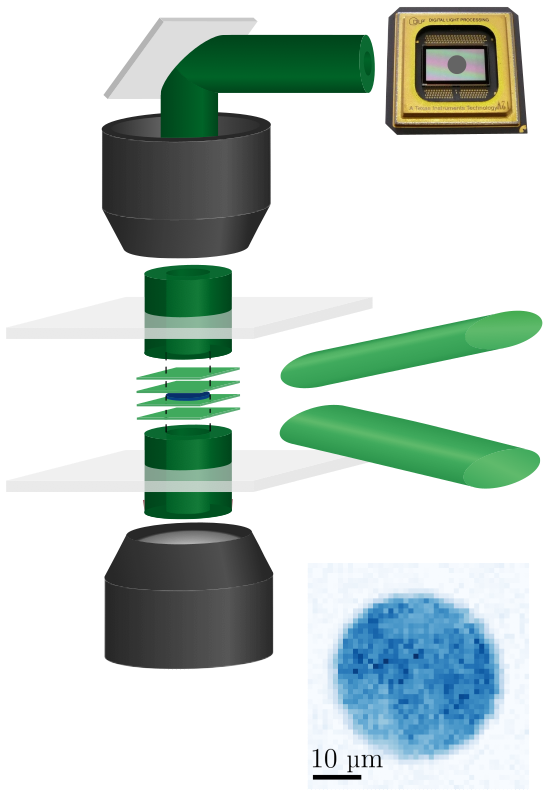
\includegraphics[height=7.5cm]{img/accordeon-dmd.png}
\begin{overpic}[percent,scale=0.35,tics=5]{img/accordeon-dmd.png}
    \put(51,79){DMD}
    \put(34,74){objectif de}
    \put(34,70){microscope}
    \put(34,64){paroi}
\end{overpic}
\end{columns}
\end{frame}

\begin{frame}{Utilisation des lasers à 532~nm}
\begin{columns}
\column{0.7\linewidth}
Interaction champ électrique-dipôle électrique induit
$\rightarrow$ force de piégeage dérivant d'un potentiel (classiquement)
\[U_\mathsc{dip}(\v r) = {-\frac12 \langle \v d \cdot \v E \rangle} = -\frac{1}{2\varepsilon_0 c}\mathfrak{Re}\left(\alpha(\omega)\right) I(\v r) \]
Cycles d'absorption et réémission $\rightarrow$ force de pression de radiation $\v F = \hbar \v k \gamma,\ \gamma = \Gamma P_e$
\column{0.3\linewidth}
\tikzset{every picture/.style={scale=0.8}}
\centering
\newcommand\mysc{0 em}

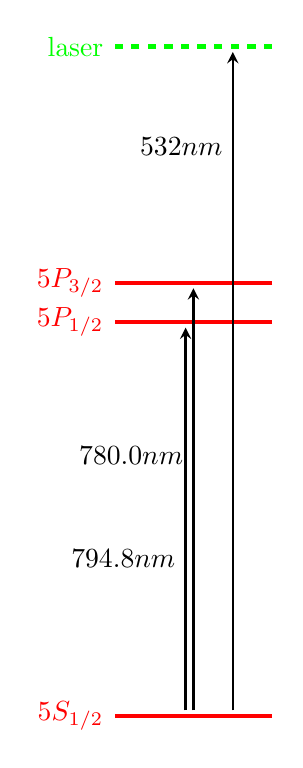
\begin{tikzpicture}[
level/.style = {
        ultra thick,
        red,
    },
    laser/.style = {
        ultra thick,
        green,
        dashed
    },
    connect/.style = {
        dashed,
        red
    },
    trans/.style={thick,->,shorten >=2pt,shorten <=2pt,>=stealth},
    notice/.style = {
        draw,
        rectangle callout,
        callout relative pointer={#1}
    },
    label/.style = {
        text width=2cm
    }
]

    % Draw all levels
    \draw[level] (0,0) --  +(-2,0) node[left] {$5S_{1/2}$} ;
    \draw[level] (0,5) --  +(-2,0) node[left] {$5P_{1/2}$} ;
    \draw[level] (0,5.5) --  +(-2,0) node[left] {$5P_{3/2}$};
    \draw[laser] (0,8.5) --  +(-2,0) node[left] {laser};
    
    \draw[trans] (-1.1,0) -- +(0,5) node[pos=0.4,left] {$\SI{794.8}{nm}$}; %794.8
    \draw[trans] (-1,0) -- +(0,5.5) node[pos=0.6,left] {$\SI{780.0}{nm}$}; %780.0
    \draw[trans] (-0.5,0) -- +(0,8.5) node[pos=0.85,left] {$\SI{532}{nm}$};
    
\end{tikzpicture}

\end{columns}
\end{frame}

\section{Principe de la génération}

\begin{frame}[plain,noframenumbering]
\begin{figure}[htbp]
  \centering
  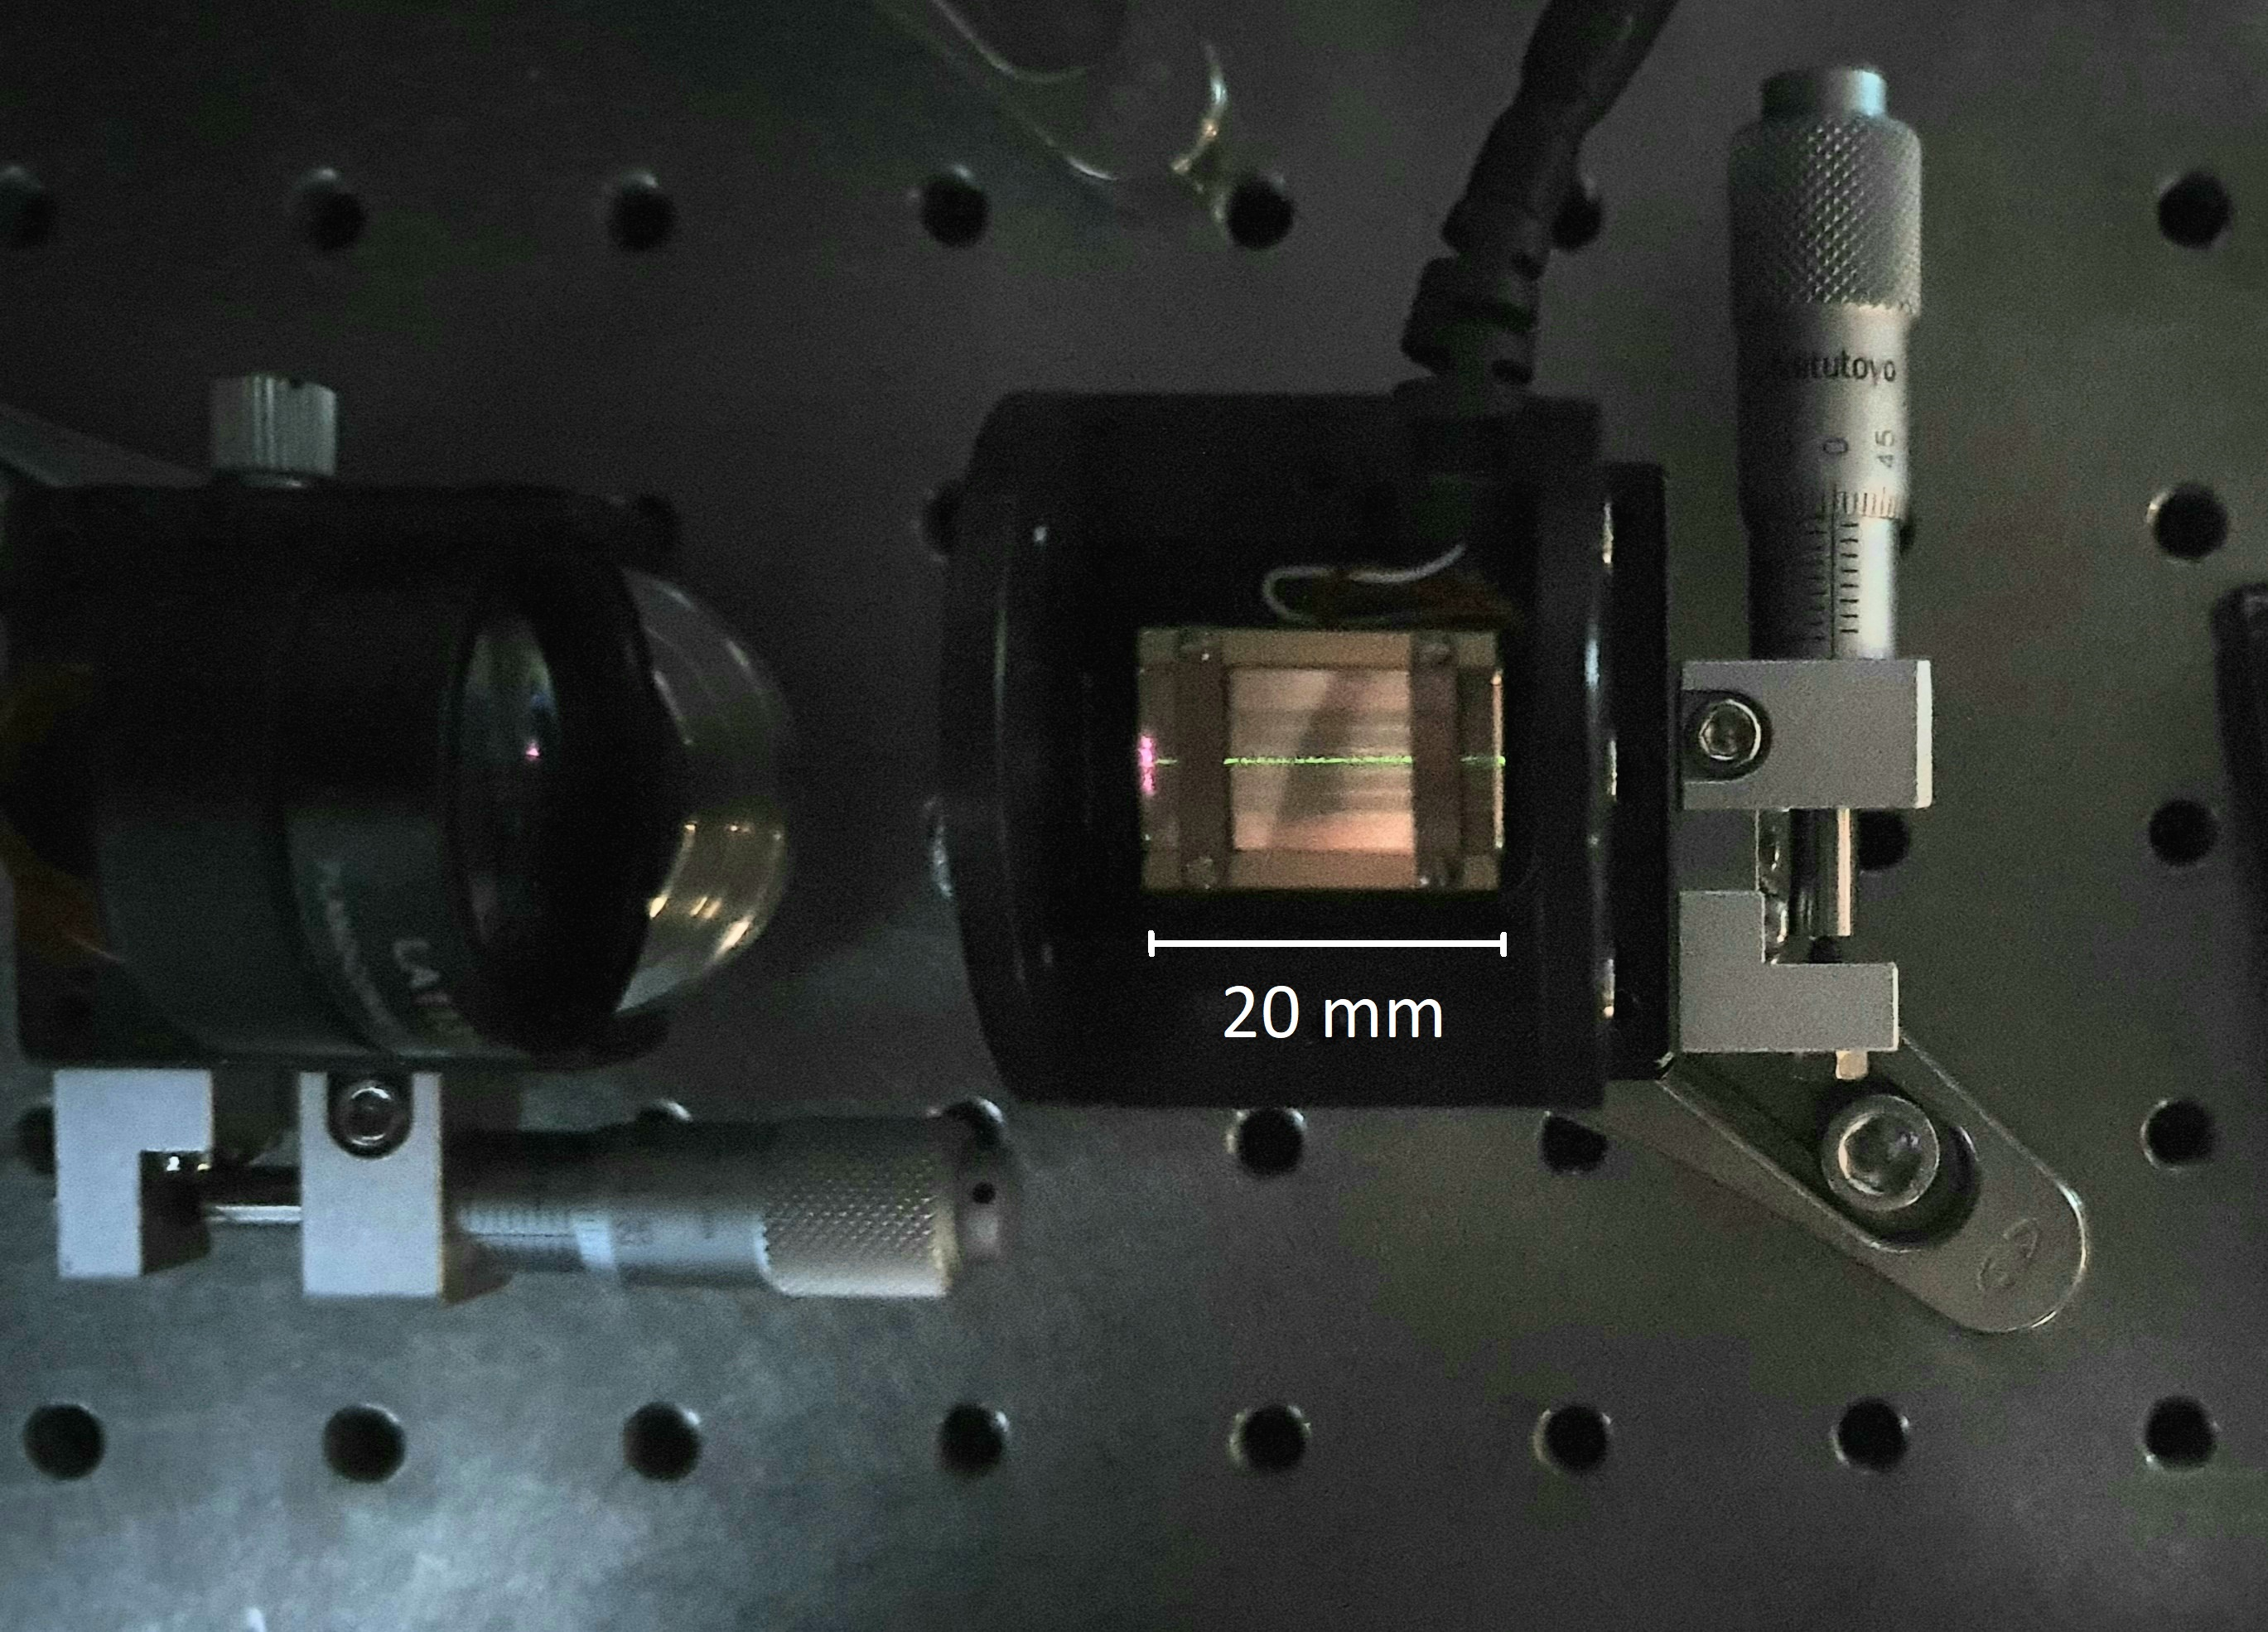
\includegraphics[width=0.7\linewidth]{img/cristal clair.jpg}
\end{figure}
\end{frame}

\begin{frame}{Milieu non linéaire}
Équation d'onde dans un milieu non magnétique non linéaire :
\begin{equation*}
\boldsymbol{\nabla}^2 \boldsymbol{\E}_q + \frac{\omega_q^2}{c^2}\tens\epsilon^{(1)}(\omega_q)\cdot \v \E_q(\v r) = \uline{red}{ - \frac{\omega_q^2}{\epsilon_0 c^2} \boldsymbol{\mathcal{P}}^\mathsc{NL}_q(\v r) }
\end{equation*}
avec
\begin{enumerate}
\item[ ] $\v E(\v r, t) = \mathfrak{Re} \left\{ \sum_{q \in \mathbb N} \v {\boldsymbol{\mathcal E}}_q (\v r) \e{-i \omega_q t} \right\}$
\item[ ] $\v P^\mathsc{NL} (\v r, t) = \mathfrak{Re} \left\{ \sum_{q \in \mathbb N} \v {\boldsymbol{\mathcal P}}^\mathsc{NL}_q (\v r) \e{-i \omega_q t} \right\}$
\item[ ] $\tens \epsilon^{(1)}$ le tenseur de permittivité diélectrique relative (linéaire)
\item[ ] $\v P^\mathsc{NL}_q$ la partie non-linéaire de la polarisation
%TODO bold font
\end{enumerate}
\end{frame}

\begin{frame}{Génération de seconde harmonique}
Polarisation quadratique pour une onde incidente à la pulsation $\omega$ $\v E = \mathfrak{Re} \left\{ \E_1 \e{-i\omega t} \right\}$
\begin{align*}
\v P^{(2)} &= \varepsilon_0 \chi^{(2)} \v E^2 \text{ avec $\chi^{(2)}$ la susceptibilité d'ordre 2}\\
&= \frac{\varepsilon_0 \chi^{(2)}}{4} \left\{\mathcal E_1 e^{-i\omega t} + \mathcal E_1^* e^{i\omega t} \vphantom{\frac12}\right\}^2 \\
&= \frac{\varepsilon_0 \chi^{(2)}}{4} \left\{\ubrace{red}{\mathcal E_1^2 \e{-2i\omega t} + \E_1^{*2} \e{2i\omega t}}{seconde harmonique}
\color{gray} + 2|\mathcal E_1|^2 + \mathcal O(\E_2^2) \vphantom{\frac12} \right\} 
\end{align*}
\end{frame}

\begin{frame}{Équation d'évolution}
Hypothèses simplificatrices :
\begin{itemize}
\item polarisation linéaire selon l'un des axes principaux
\item[$\rightarrow$] $\E_q$ scalaires, $n_q = \sqrt{ \varepsilon^{(1)}(\omega_q)}$
\item $\E_q = \A_q(x,y,z) \e{ik_qz}$ avec $k_q =\frac{n_q \omega_q}{c}$ et $\frac{\partial^2 \A_q}{\partial z^2} \ll k_q \frac{\partial \A_q}{\partial z}$
\end{itemize}
$\boldsymbol \rightarrow$ équation d'onde paraxiale avec terme source quadratique en $\A_1$
\begin{equation*}
\left\{\v\nabla_\bot + 2 i k_2 \frac{\partial}{\partial z} \right\} \A_2 = - \frac{2 \chi^{(2)} \omega^2}{c^2} \A_1^2 \e{- i (k_2 - 2k_1) z}
\end{equation*}
\end{frame}

\begin{frame}{Accord de phase}
Pour des ondes planes $\A_q = \A_q(z)$,
\begin{align*}
	\dv{\A_2}{z} &= i\frac{\chi^{(2)}\omega}{2cn_2} \A_1^2 \e{-i \Delta k z} \text{ avec } {\Delta k = k_2 - 2k_1} \label{eq:pwe} \\
	\text{soit } \A_2(L) &= i \frac{\chi^{(2)}\omega}{2 cn_2} \A_1^2 L\, \uline{red}{\operatorname{sinc}\left( \frac{\Delta k L}{2} \right)}\, \e{-i\frac{\Delta k L}{2}}
\end{align*}
en sortie du cristal en $z=L$ avec $\A_2(0)=0$ à l'entrée.
\end{frame}

\begin{frame}{Accord de phase}
Interférence destructive du rayonnement émis en $z$ et en  $z+L_\mathsc{coh} := z + \frac{\pi}{\Delta k}$. $L_\mathsc{coh} \approx \SI{3}{\micro\meter} \ll L = \SI{2}{cm}$.
\begin{figure}
\centering
% This file was created with tikzplotlib v0.10.1.
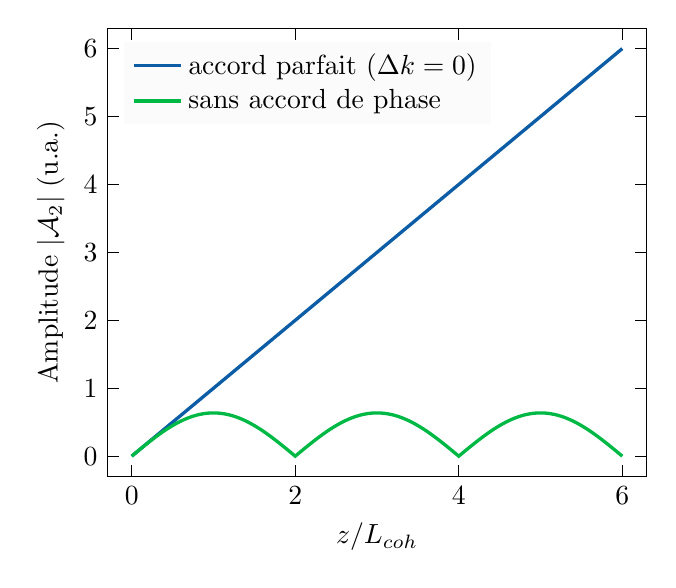
\begin{tikzpicture}

\definecolor{darkgray176}{RGB}{176,176,176}
\definecolor{darkorange2551490}{RGB}{255,149,0}
\definecolor{limegreen018569}{RGB}{0,185,69}
\definecolor{orangered255440}{RGB}{255,44,0}
\definecolor{teal1293165}{RGB}{12,93,165}

\begin{axis}[
legend cell align={left},
legend style={
	fill=black!2,
  fill opacity=0.8,
  draw opacity=1,
  text opacity=1,
  at={(0.03,0.97)},
  anchor=north west,
  draw=none
},
tick pos=both,
x grid style={darkgray176},
xlabel={\(\displaystyle z/L_\text{coh}\)},
xmin=-0.3, xmax=6.3,
xtick style={color=black},
xtick={-2,0,2,4,6,8},
xticklabels={
  \(\displaystyle {\ensuremath{-}2}\),
  \(\displaystyle {0}\),
  \(\displaystyle {2}\),
  \(\displaystyle {4}\),
  \(\displaystyle {6}\),
  \(\displaystyle {8}\)
},
y grid style={darkgray176},
ylabel={Amplitude \(\displaystyle \left|\mathcal A_2\right| \) (u.a.)},
ymin=-0.3, ymax=6.3,
ytick style={color=black},
ytick={-1,0,1,2,3,4,5,6,7},
yticklabels={
  \(\displaystyle {\ensuremath{-}1}\),
  \(\displaystyle {0}\),
  \(\displaystyle {1}\),
  \(\displaystyle {2}\),
  \(\displaystyle {3}\),
  \(\displaystyle {4}\),
  \(\displaystyle {5}\),
  \(\displaystyle {6}\),
  \(\displaystyle {7}\)
}
]
\addplot [very thick, teal1293165]
table {%
0 0
0.00600600600600601 0.00600600600600601
0.012012012012012 0.012012012012012
0.018018018018018 0.018018018018018
0.024024024024024 0.024024024024024
0.03003003003003 0.03003003003003
0.036036036036036 0.036036036036036
0.042042042042042 0.042042042042042
0.048048048048048 0.048048048048048
0.0540540540540541 0.0540540540540541
0.0600600600600601 0.0600600600600601
0.0660660660660661 0.0660660660660661
0.0720720720720721 0.0720720720720721
0.0780780780780781 0.0780780780780781
0.0840840840840841 0.0840840840840841
0.0900900900900901 0.0900900900900901
0.0960960960960961 0.0960960960960961
0.102102102102102 0.102102102102102
0.108108108108108 0.108108108108108
0.114114114114114 0.114114114114114
0.12012012012012 0.12012012012012
0.126126126126126 0.126126126126126
0.132132132132132 0.132132132132132
0.138138138138138 0.138138138138138
0.144144144144144 0.144144144144144
0.15015015015015 0.15015015015015
0.156156156156156 0.156156156156156
0.162162162162162 0.162162162162162
0.168168168168168 0.168168168168168
0.174174174174174 0.174174174174174
0.18018018018018 0.18018018018018
0.186186186186186 0.186186186186186
0.192192192192192 0.192192192192192
0.198198198198198 0.198198198198198
0.204204204204204 0.204204204204204
0.21021021021021 0.21021021021021
0.216216216216216 0.216216216216216
0.222222222222222 0.222222222222222
0.228228228228228 0.228228228228228
0.234234234234234 0.234234234234234
0.24024024024024 0.24024024024024
0.246246246246246 0.246246246246246
0.252252252252252 0.252252252252252
0.258258258258258 0.258258258258258
0.264264264264264 0.264264264264264
0.27027027027027 0.27027027027027
0.276276276276276 0.276276276276276
0.282282282282282 0.282282282282282
0.288288288288288 0.288288288288288
0.294294294294294 0.294294294294294
0.3003003003003 0.3003003003003
0.306306306306306 0.306306306306306
0.312312312312312 0.312312312312312
0.318318318318318 0.318318318318318
0.324324324324324 0.324324324324324
0.33033033033033 0.33033033033033
0.336336336336336 0.336336336336336
0.342342342342342 0.342342342342342
0.348348348348348 0.348348348348348
0.354354354354354 0.354354354354354
0.36036036036036 0.36036036036036
0.366366366366366 0.366366366366366
0.372372372372372 0.372372372372372
0.378378378378378 0.378378378378378
0.384384384384384 0.384384384384384
0.39039039039039 0.39039039039039
0.396396396396396 0.396396396396396
0.402402402402402 0.402402402402402
0.408408408408408 0.408408408408408
0.414414414414414 0.414414414414414
0.42042042042042 0.42042042042042
0.426426426426426 0.426426426426426
0.432432432432432 0.432432432432432
0.438438438438438 0.438438438438438
0.444444444444444 0.444444444444444
0.45045045045045 0.45045045045045
0.456456456456456 0.456456456456456
0.462462462462462 0.462462462462462
0.468468468468468 0.468468468468468
0.474474474474474 0.474474474474474
0.48048048048048 0.48048048048048
0.486486486486486 0.486486486486486
0.492492492492492 0.492492492492492
0.498498498498498 0.498498498498498
0.504504504504504 0.504504504504504
0.510510510510511 0.510510510510511
0.516516516516517 0.516516516516517
0.522522522522523 0.522522522522523
0.528528528528528 0.528528528528528
0.534534534534534 0.534534534534534
0.540540540540541 0.540540540540541
0.546546546546547 0.546546546546547
0.552552552552553 0.552552552552553
0.558558558558559 0.558558558558559
0.564564564564565 0.564564564564565
0.570570570570571 0.570570570570571
0.576576576576577 0.576576576576577
0.582582582582583 0.582582582582583
0.588588588588589 0.588588588588589
0.594594594594595 0.594594594594595
0.600600600600601 0.600600600600601
0.606606606606607 0.606606606606607
0.612612612612613 0.612612612612613
0.618618618618619 0.618618618618619
0.624624624624625 0.624624624624625
0.630630630630631 0.630630630630631
0.636636636636637 0.636636636636637
0.642642642642643 0.642642642642643
0.648648648648649 0.648648648648649
0.654654654654655 0.654654654654655
0.660660660660661 0.660660660660661
0.666666666666667 0.666666666666667
0.672672672672673 0.672672672672673
0.678678678678679 0.678678678678679
0.684684684684685 0.684684684684685
0.690690690690691 0.690690690690691
0.696696696696697 0.696696696696697
0.702702702702703 0.702702702702703
0.708708708708709 0.708708708708709
0.714714714714715 0.714714714714715
0.720720720720721 0.720720720720721
0.726726726726727 0.726726726726727
0.732732732732733 0.732732732732733
0.738738738738739 0.738738738738739
0.744744744744745 0.744744744744745
0.750750750750751 0.750750750750751
0.756756756756757 0.756756756756757
0.762762762762763 0.762762762762763
0.768768768768769 0.768768768768769
0.774774774774775 0.774774774774775
0.780780780780781 0.780780780780781
0.786786786786787 0.786786786786787
0.792792792792793 0.792792792792793
0.798798798798799 0.798798798798799
0.804804804804805 0.804804804804805
0.810810810810811 0.810810810810811
0.816816816816817 0.816816816816817
0.822822822822823 0.822822822822823
0.828828828828829 0.828828828828829
0.834834834834835 0.834834834834835
0.840840840840841 0.840840840840841
0.846846846846847 0.846846846846847
0.852852852852853 0.852852852852853
0.858858858858859 0.858858858858859
0.864864864864865 0.864864864864865
0.870870870870871 0.870870870870871
0.876876876876877 0.876876876876877
0.882882882882883 0.882882882882883
0.888888888888889 0.888888888888889
0.894894894894895 0.894894894894895
0.900900900900901 0.900900900900901
0.906906906906907 0.906906906906907
0.912912912912913 0.912912912912913
0.918918918918919 0.918918918918919
0.924924924924925 0.924924924924925
0.930930930930931 0.930930930930931
0.936936936936937 0.936936936936937
0.942942942942943 0.942942942942943
0.948948948948949 0.948948948948949
0.954954954954955 0.954954954954955
0.960960960960961 0.960960960960961
0.966966966966967 0.966966966966967
0.972972972972973 0.972972972972973
0.978978978978979 0.978978978978979
0.984984984984985 0.984984984984985
0.990990990990991 0.990990990990991
0.996996996996997 0.996996996996997
1.003003003003 1.003003003003
1.00900900900901 1.00900900900901
1.01501501501502 1.01501501501502
1.02102102102102 1.02102102102102
1.02702702702703 1.02702702702703
1.03303303303303 1.03303303303303
1.03903903903904 1.03903903903904
1.04504504504505 1.04504504504505
1.05105105105105 1.05105105105105
1.05705705705706 1.05705705705706
1.06306306306306 1.06306306306306
1.06906906906907 1.06906906906907
1.07507507507508 1.07507507507508
1.08108108108108 1.08108108108108
1.08708708708709 1.08708708708709
1.09309309309309 1.09309309309309
1.0990990990991 1.0990990990991
1.10510510510511 1.10510510510511
1.11111111111111 1.11111111111111
1.11711711711712 1.11711711711712
1.12312312312312 1.12312312312312
1.12912912912913 1.12912912912913
1.13513513513514 1.13513513513514
1.14114114114114 1.14114114114114
1.14714714714715 1.14714714714715
1.15315315315315 1.15315315315315
1.15915915915916 1.15915915915916
1.16516516516517 1.16516516516517
1.17117117117117 1.17117117117117
1.17717717717718 1.17717717717718
1.18318318318318 1.18318318318318
1.18918918918919 1.18918918918919
1.1951951951952 1.1951951951952
1.2012012012012 1.2012012012012
1.20720720720721 1.20720720720721
1.21321321321321 1.21321321321321
1.21921921921922 1.21921921921922
1.22522522522523 1.22522522522523
1.23123123123123 1.23123123123123
1.23723723723724 1.23723723723724
1.24324324324324 1.24324324324324
1.24924924924925 1.24924924924925
1.25525525525526 1.25525525525526
1.26126126126126 1.26126126126126
1.26726726726727 1.26726726726727
1.27327327327327 1.27327327327327
1.27927927927928 1.27927927927928
1.28528528528529 1.28528528528529
1.29129129129129 1.29129129129129
1.2972972972973 1.2972972972973
1.3033033033033 1.3033033033033
1.30930930930931 1.30930930930931
1.31531531531532 1.31531531531532
1.32132132132132 1.32132132132132
1.32732732732733 1.32732732732733
1.33333333333333 1.33333333333333
1.33933933933934 1.33933933933934
1.34534534534535 1.34534534534535
1.35135135135135 1.35135135135135
1.35735735735736 1.35735735735736
1.36336336336336 1.36336336336336
1.36936936936937 1.36936936936937
1.37537537537538 1.37537537537538
1.38138138138138 1.38138138138138
1.38738738738739 1.38738738738739
1.39339339339339 1.39339339339339
1.3993993993994 1.3993993993994
1.40540540540541 1.40540540540541
1.41141141141141 1.41141141141141
1.41741741741742 1.41741741741742
1.42342342342342 1.42342342342342
1.42942942942943 1.42942942942943
1.43543543543544 1.43543543543544
1.44144144144144 1.44144144144144
1.44744744744745 1.44744744744745
1.45345345345345 1.45345345345345
1.45945945945946 1.45945945945946
1.46546546546547 1.46546546546547
1.47147147147147 1.47147147147147
1.47747747747748 1.47747747747748
1.48348348348348 1.48348348348348
1.48948948948949 1.48948948948949
1.4954954954955 1.4954954954955
1.5015015015015 1.5015015015015
1.50750750750751 1.50750750750751
1.51351351351351 1.51351351351351
1.51951951951952 1.51951951951952
1.52552552552553 1.52552552552553
1.53153153153153 1.53153153153153
1.53753753753754 1.53753753753754
1.54354354354354 1.54354354354354
1.54954954954955 1.54954954954955
1.55555555555556 1.55555555555556
1.56156156156156 1.56156156156156
1.56756756756757 1.56756756756757
1.57357357357357 1.57357357357357
1.57957957957958 1.57957957957958
1.58558558558559 1.58558558558559
1.59159159159159 1.59159159159159
1.5975975975976 1.5975975975976
1.6036036036036 1.6036036036036
1.60960960960961 1.60960960960961
1.61561561561562 1.61561561561562
1.62162162162162 1.62162162162162
1.62762762762763 1.62762762762763
1.63363363363363 1.63363363363363
1.63963963963964 1.63963963963964
1.64564564564565 1.64564564564565
1.65165165165165 1.65165165165165
1.65765765765766 1.65765765765766
1.66366366366366 1.66366366366366
1.66966966966967 1.66966966966967
1.67567567567568 1.67567567567568
1.68168168168168 1.68168168168168
1.68768768768769 1.68768768768769
1.69369369369369 1.69369369369369
1.6996996996997 1.6996996996997
1.70570570570571 1.70570570570571
1.71171171171171 1.71171171171171
1.71771771771772 1.71771771771772
1.72372372372372 1.72372372372372
1.72972972972973 1.72972972972973
1.73573573573574 1.73573573573574
1.74174174174174 1.74174174174174
1.74774774774775 1.74774774774775
1.75375375375375 1.75375375375375
1.75975975975976 1.75975975975976
1.76576576576577 1.76576576576577
1.77177177177177 1.77177177177177
1.77777777777778 1.77777777777778
1.78378378378378 1.78378378378378
1.78978978978979 1.78978978978979
1.7957957957958 1.7957957957958
1.8018018018018 1.8018018018018
1.80780780780781 1.80780780780781
1.81381381381381 1.81381381381381
1.81981981981982 1.81981981981982
1.82582582582583 1.82582582582583
1.83183183183183 1.83183183183183
1.83783783783784 1.83783783783784
1.84384384384384 1.84384384384384
1.84984984984985 1.84984984984985
1.85585585585586 1.85585585585586
1.86186186186186 1.86186186186186
1.86786786786787 1.86786786786787
1.87387387387387 1.87387387387387
1.87987987987988 1.87987987987988
1.88588588588589 1.88588588588589
1.89189189189189 1.89189189189189
1.8978978978979 1.8978978978979
1.9039039039039 1.9039039039039
1.90990990990991 1.90990990990991
1.91591591591592 1.91591591591592
1.92192192192192 1.92192192192192
1.92792792792793 1.92792792792793
1.93393393393393 1.93393393393393
1.93993993993994 1.93993993993994
1.94594594594595 1.94594594594595
1.95195195195195 1.95195195195195
1.95795795795796 1.95795795795796
1.96396396396396 1.96396396396396
1.96996996996997 1.96996996996997
1.97597597597598 1.97597597597598
1.98198198198198 1.98198198198198
1.98798798798799 1.98798798798799
1.99399399399399 1.99399399399399
2 2
2.00600600600601 2.00600600600601
2.01201201201201 2.01201201201201
2.01801801801802 2.01801801801802
2.02402402402402 2.02402402402402
2.03003003003003 2.03003003003003
2.03603603603604 2.03603603603604
2.04204204204204 2.04204204204204
2.04804804804805 2.04804804804805
2.05405405405405 2.05405405405405
2.06006006006006 2.06006006006006
2.06606606606607 2.06606606606607
2.07207207207207 2.07207207207207
2.07807807807808 2.07807807807808
2.08408408408408 2.08408408408408
2.09009009009009 2.09009009009009
2.0960960960961 2.0960960960961
2.1021021021021 2.1021021021021
2.10810810810811 2.10810810810811
2.11411411411411 2.11411411411411
2.12012012012012 2.12012012012012
2.12612612612613 2.12612612612613
2.13213213213213 2.13213213213213
2.13813813813814 2.13813813813814
2.14414414414414 2.14414414414414
2.15015015015015 2.15015015015015
2.15615615615616 2.15615615615616
2.16216216216216 2.16216216216216
2.16816816816817 2.16816816816817
2.17417417417417 2.17417417417417
2.18018018018018 2.18018018018018
2.18618618618619 2.18618618618619
2.19219219219219 2.19219219219219
2.1981981981982 2.1981981981982
2.2042042042042 2.2042042042042
2.21021021021021 2.21021021021021
2.21621621621622 2.21621621621622
2.22222222222222 2.22222222222222
2.22822822822823 2.22822822822823
2.23423423423423 2.23423423423423
2.24024024024024 2.24024024024024
2.24624624624625 2.24624624624625
2.25225225225225 2.25225225225225
2.25825825825826 2.25825825825826
2.26426426426426 2.26426426426426
2.27027027027027 2.27027027027027
2.27627627627628 2.27627627627628
2.28228228228228 2.28228228228228
2.28828828828829 2.28828828828829
2.29429429429429 2.29429429429429
2.3003003003003 2.3003003003003
2.30630630630631 2.30630630630631
2.31231231231231 2.31231231231231
2.31831831831832 2.31831831831832
2.32432432432432 2.32432432432432
2.33033033033033 2.33033033033033
2.33633633633634 2.33633633633634
2.34234234234234 2.34234234234234
2.34834834834835 2.34834834834835
2.35435435435435 2.35435435435435
2.36036036036036 2.36036036036036
2.36636636636637 2.36636636636637
2.37237237237237 2.37237237237237
2.37837837837838 2.37837837837838
2.38438438438438 2.38438438438438
2.39039039039039 2.39039039039039
2.3963963963964 2.3963963963964
2.4024024024024 2.4024024024024
2.40840840840841 2.40840840840841
2.41441441441441 2.41441441441441
2.42042042042042 2.42042042042042
2.42642642642643 2.42642642642643
2.43243243243243 2.43243243243243
2.43843843843844 2.43843843843844
2.44444444444444 2.44444444444444
2.45045045045045 2.45045045045045
2.45645645645646 2.45645645645646
2.46246246246246 2.46246246246246
2.46846846846847 2.46846846846847
2.47447447447447 2.47447447447447
2.48048048048048 2.48048048048048
2.48648648648649 2.48648648648649
2.49249249249249 2.49249249249249
2.4984984984985 2.4984984984985
2.5045045045045 2.5045045045045
2.51051051051051 2.51051051051051
2.51651651651652 2.51651651651652
2.52252252252252 2.52252252252252
2.52852852852853 2.52852852852853
2.53453453453453 2.53453453453453
2.54054054054054 2.54054054054054
2.54654654654655 2.54654654654655
2.55255255255255 2.55255255255255
2.55855855855856 2.55855855855856
2.56456456456456 2.56456456456456
2.57057057057057 2.57057057057057
2.57657657657658 2.57657657657658
2.58258258258258 2.58258258258258
2.58858858858859 2.58858858858859
2.59459459459459 2.59459459459459
2.6006006006006 2.6006006006006
2.60660660660661 2.60660660660661
2.61261261261261 2.61261261261261
2.61861861861862 2.61861861861862
2.62462462462462 2.62462462462462
2.63063063063063 2.63063063063063
2.63663663663664 2.63663663663664
2.64264264264264 2.64264264264264
2.64864864864865 2.64864864864865
2.65465465465465 2.65465465465465
2.66066066066066 2.66066066066066
2.66666666666667 2.66666666666667
2.67267267267267 2.67267267267267
2.67867867867868 2.67867867867868
2.68468468468468 2.68468468468468
2.69069069069069 2.69069069069069
2.6966966966967 2.6966966966967
2.7027027027027 2.7027027027027
2.70870870870871 2.70870870870871
2.71471471471471 2.71471471471471
2.72072072072072 2.72072072072072
2.72672672672673 2.72672672672673
2.73273273273273 2.73273273273273
2.73873873873874 2.73873873873874
2.74474474474474 2.74474474474474
2.75075075075075 2.75075075075075
2.75675675675676 2.75675675675676
2.76276276276276 2.76276276276276
2.76876876876877 2.76876876876877
2.77477477477477 2.77477477477477
2.78078078078078 2.78078078078078
2.78678678678679 2.78678678678679
2.79279279279279 2.79279279279279
2.7987987987988 2.7987987987988
2.8048048048048 2.8048048048048
2.81081081081081 2.81081081081081
2.81681681681682 2.81681681681682
2.82282282282282 2.82282282282282
2.82882882882883 2.82882882882883
2.83483483483483 2.83483483483483
2.84084084084084 2.84084084084084
2.84684684684685 2.84684684684685
2.85285285285285 2.85285285285285
2.85885885885886 2.85885885885886
2.86486486486486 2.86486486486486
2.87087087087087 2.87087087087087
2.87687687687688 2.87687687687688
2.88288288288288 2.88288288288288
2.88888888888889 2.88888888888889
2.89489489489489 2.89489489489489
2.9009009009009 2.9009009009009
2.90690690690691 2.90690690690691
2.91291291291291 2.91291291291291
2.91891891891892 2.91891891891892
2.92492492492492 2.92492492492492
2.93093093093093 2.93093093093093
2.93693693693694 2.93693693693694
2.94294294294294 2.94294294294294
2.94894894894895 2.94894894894895
2.95495495495495 2.95495495495495
2.96096096096096 2.96096096096096
2.96696696696697 2.96696696696697
2.97297297297297 2.97297297297297
2.97897897897898 2.97897897897898
2.98498498498498 2.98498498498498
2.99099099099099 2.99099099099099
2.996996996997 2.996996996997
3.003003003003 3.003003003003
3.00900900900901 3.00900900900901
3.01501501501502 3.01501501501502
3.02102102102102 3.02102102102102
3.02702702702703 3.02702702702703
3.03303303303303 3.03303303303303
3.03903903903904 3.03903903903904
3.04504504504505 3.04504504504505
3.05105105105105 3.05105105105105
3.05705705705706 3.05705705705706
3.06306306306306 3.06306306306306
3.06906906906907 3.06906906906907
3.07507507507508 3.07507507507508
3.08108108108108 3.08108108108108
3.08708708708709 3.08708708708709
3.09309309309309 3.09309309309309
3.0990990990991 3.0990990990991
3.10510510510511 3.10510510510511
3.11111111111111 3.11111111111111
3.11711711711712 3.11711711711712
3.12312312312312 3.12312312312312
3.12912912912913 3.12912912912913
3.13513513513514 3.13513513513514
3.14114114114114 3.14114114114114
3.14714714714715 3.14714714714715
3.15315315315315 3.15315315315315
3.15915915915916 3.15915915915916
3.16516516516517 3.16516516516517
3.17117117117117 3.17117117117117
3.17717717717718 3.17717717717718
3.18318318318318 3.18318318318318
3.18918918918919 3.18918918918919
3.1951951951952 3.1951951951952
3.2012012012012 3.2012012012012
3.20720720720721 3.20720720720721
3.21321321321321 3.21321321321321
3.21921921921922 3.21921921921922
3.22522522522523 3.22522522522523
3.23123123123123 3.23123123123123
3.23723723723724 3.23723723723724
3.24324324324324 3.24324324324324
3.24924924924925 3.24924924924925
3.25525525525526 3.25525525525526
3.26126126126126 3.26126126126126
3.26726726726727 3.26726726726727
3.27327327327327 3.27327327327327
3.27927927927928 3.27927927927928
3.28528528528529 3.28528528528529
3.29129129129129 3.29129129129129
3.2972972972973 3.2972972972973
3.3033033033033 3.3033033033033
3.30930930930931 3.30930930930931
3.31531531531532 3.31531531531532
3.32132132132132 3.32132132132132
3.32732732732733 3.32732732732733
3.33333333333333 3.33333333333333
3.33933933933934 3.33933933933934
3.34534534534535 3.34534534534535
3.35135135135135 3.35135135135135
3.35735735735736 3.35735735735736
3.36336336336336 3.36336336336336
3.36936936936937 3.36936936936937
3.37537537537538 3.37537537537538
3.38138138138138 3.38138138138138
3.38738738738739 3.38738738738739
3.39339339339339 3.39339339339339
3.3993993993994 3.3993993993994
3.40540540540541 3.40540540540541
3.41141141141141 3.41141141141141
3.41741741741742 3.41741741741742
3.42342342342342 3.42342342342342
3.42942942942943 3.42942942942943
3.43543543543544 3.43543543543544
3.44144144144144 3.44144144144144
3.44744744744745 3.44744744744745
3.45345345345345 3.45345345345345
3.45945945945946 3.45945945945946
3.46546546546547 3.46546546546547
3.47147147147147 3.47147147147147
3.47747747747748 3.47747747747748
3.48348348348348 3.48348348348348
3.48948948948949 3.48948948948949
3.4954954954955 3.4954954954955
3.5015015015015 3.5015015015015
3.50750750750751 3.50750750750751
3.51351351351351 3.51351351351351
3.51951951951952 3.51951951951952
3.52552552552553 3.52552552552553
3.53153153153153 3.53153153153153
3.53753753753754 3.53753753753754
3.54354354354354 3.54354354354354
3.54954954954955 3.54954954954955
3.55555555555556 3.55555555555556
3.56156156156156 3.56156156156156
3.56756756756757 3.56756756756757
3.57357357357357 3.57357357357357
3.57957957957958 3.57957957957958
3.58558558558559 3.58558558558559
3.59159159159159 3.59159159159159
3.5975975975976 3.5975975975976
3.6036036036036 3.6036036036036
3.60960960960961 3.60960960960961
3.61561561561562 3.61561561561562
3.62162162162162 3.62162162162162
3.62762762762763 3.62762762762763
3.63363363363363 3.63363363363363
3.63963963963964 3.63963963963964
3.64564564564565 3.64564564564565
3.65165165165165 3.65165165165165
3.65765765765766 3.65765765765766
3.66366366366366 3.66366366366366
3.66966966966967 3.66966966966967
3.67567567567568 3.67567567567568
3.68168168168168 3.68168168168168
3.68768768768769 3.68768768768769
3.69369369369369 3.69369369369369
3.6996996996997 3.6996996996997
3.70570570570571 3.70570570570571
3.71171171171171 3.71171171171171
3.71771771771772 3.71771771771772
3.72372372372372 3.72372372372372
3.72972972972973 3.72972972972973
3.73573573573574 3.73573573573574
3.74174174174174 3.74174174174174
3.74774774774775 3.74774774774775
3.75375375375375 3.75375375375375
3.75975975975976 3.75975975975976
3.76576576576577 3.76576576576577
3.77177177177177 3.77177177177177
3.77777777777778 3.77777777777778
3.78378378378378 3.78378378378378
3.78978978978979 3.78978978978979
3.7957957957958 3.7957957957958
3.8018018018018 3.8018018018018
3.80780780780781 3.80780780780781
3.81381381381381 3.81381381381381
3.81981981981982 3.81981981981982
3.82582582582583 3.82582582582583
3.83183183183183 3.83183183183183
3.83783783783784 3.83783783783784
3.84384384384384 3.84384384384384
3.84984984984985 3.84984984984985
3.85585585585586 3.85585585585586
3.86186186186186 3.86186186186186
3.86786786786787 3.86786786786787
3.87387387387387 3.87387387387387
3.87987987987988 3.87987987987988
3.88588588588589 3.88588588588589
3.89189189189189 3.89189189189189
3.8978978978979 3.8978978978979
3.9039039039039 3.9039039039039
3.90990990990991 3.90990990990991
3.91591591591592 3.91591591591592
3.92192192192192 3.92192192192192
3.92792792792793 3.92792792792793
3.93393393393393 3.93393393393393
3.93993993993994 3.93993993993994
3.94594594594595 3.94594594594595
3.95195195195195 3.95195195195195
3.95795795795796 3.95795795795796
3.96396396396396 3.96396396396396
3.96996996996997 3.96996996996997
3.97597597597598 3.97597597597598
3.98198198198198 3.98198198198198
3.98798798798799 3.98798798798799
3.99399399399399 3.99399399399399
4 4
4.00600600600601 4.00600600600601
4.01201201201201 4.01201201201201
4.01801801801802 4.01801801801802
4.02402402402402 4.02402402402402
4.03003003003003 4.03003003003003
4.03603603603604 4.03603603603604
4.04204204204204 4.04204204204204
4.04804804804805 4.04804804804805
4.05405405405405 4.05405405405405
4.06006006006006 4.06006006006006
4.06606606606607 4.06606606606607
4.07207207207207 4.07207207207207
4.07807807807808 4.07807807807808
4.08408408408408 4.08408408408408
4.09009009009009 4.09009009009009
4.0960960960961 4.0960960960961
4.1021021021021 4.1021021021021
4.10810810810811 4.10810810810811
4.11411411411411 4.11411411411411
4.12012012012012 4.12012012012012
4.12612612612613 4.12612612612613
4.13213213213213 4.13213213213213
4.13813813813814 4.13813813813814
4.14414414414414 4.14414414414414
4.15015015015015 4.15015015015015
4.15615615615616 4.15615615615616
4.16216216216216 4.16216216216216
4.16816816816817 4.16816816816817
4.17417417417417 4.17417417417417
4.18018018018018 4.18018018018018
4.18618618618619 4.18618618618619
4.19219219219219 4.19219219219219
4.1981981981982 4.1981981981982
4.2042042042042 4.2042042042042
4.21021021021021 4.21021021021021
4.21621621621622 4.21621621621622
4.22222222222222 4.22222222222222
4.22822822822823 4.22822822822823
4.23423423423423 4.23423423423423
4.24024024024024 4.24024024024024
4.24624624624625 4.24624624624625
4.25225225225225 4.25225225225225
4.25825825825826 4.25825825825826
4.26426426426426 4.26426426426426
4.27027027027027 4.27027027027027
4.27627627627628 4.27627627627628
4.28228228228228 4.28228228228228
4.28828828828829 4.28828828828829
4.29429429429429 4.29429429429429
4.3003003003003 4.3003003003003
4.30630630630631 4.30630630630631
4.31231231231231 4.31231231231231
4.31831831831832 4.31831831831832
4.32432432432432 4.32432432432432
4.33033033033033 4.33033033033033
4.33633633633634 4.33633633633634
4.34234234234234 4.34234234234234
4.34834834834835 4.34834834834835
4.35435435435435 4.35435435435435
4.36036036036036 4.36036036036036
4.36636636636637 4.36636636636637
4.37237237237237 4.37237237237237
4.37837837837838 4.37837837837838
4.38438438438438 4.38438438438438
4.39039039039039 4.39039039039039
4.3963963963964 4.3963963963964
4.4024024024024 4.4024024024024
4.40840840840841 4.40840840840841
4.41441441441441 4.41441441441441
4.42042042042042 4.42042042042042
4.42642642642643 4.42642642642643
4.43243243243243 4.43243243243243
4.43843843843844 4.43843843843844
4.44444444444444 4.44444444444444
4.45045045045045 4.45045045045045
4.45645645645646 4.45645645645646
4.46246246246246 4.46246246246246
4.46846846846847 4.46846846846847
4.47447447447447 4.47447447447447
4.48048048048048 4.48048048048048
4.48648648648649 4.48648648648649
4.49249249249249 4.49249249249249
4.4984984984985 4.4984984984985
4.5045045045045 4.5045045045045
4.51051051051051 4.51051051051051
4.51651651651652 4.51651651651652
4.52252252252252 4.52252252252252
4.52852852852853 4.52852852852853
4.53453453453453 4.53453453453453
4.54054054054054 4.54054054054054
4.54654654654655 4.54654654654655
4.55255255255255 4.55255255255255
4.55855855855856 4.55855855855856
4.56456456456456 4.56456456456456
4.57057057057057 4.57057057057057
4.57657657657658 4.57657657657658
4.58258258258258 4.58258258258258
4.58858858858859 4.58858858858859
4.59459459459459 4.59459459459459
4.6006006006006 4.6006006006006
4.60660660660661 4.60660660660661
4.61261261261261 4.61261261261261
4.61861861861862 4.61861861861862
4.62462462462462 4.62462462462462
4.63063063063063 4.63063063063063
4.63663663663664 4.63663663663664
4.64264264264264 4.64264264264264
4.64864864864865 4.64864864864865
4.65465465465465 4.65465465465465
4.66066066066066 4.66066066066066
4.66666666666667 4.66666666666667
4.67267267267267 4.67267267267267
4.67867867867868 4.67867867867868
4.68468468468468 4.68468468468468
4.69069069069069 4.69069069069069
4.6966966966967 4.6966966966967
4.7027027027027 4.7027027027027
4.70870870870871 4.70870870870871
4.71471471471471 4.71471471471471
4.72072072072072 4.72072072072072
4.72672672672673 4.72672672672673
4.73273273273273 4.73273273273273
4.73873873873874 4.73873873873874
4.74474474474474 4.74474474474474
4.75075075075075 4.75075075075075
4.75675675675676 4.75675675675676
4.76276276276276 4.76276276276276
4.76876876876877 4.76876876876877
4.77477477477477 4.77477477477477
4.78078078078078 4.78078078078078
4.78678678678679 4.78678678678679
4.79279279279279 4.79279279279279
4.7987987987988 4.7987987987988
4.8048048048048 4.8048048048048
4.81081081081081 4.81081081081081
4.81681681681682 4.81681681681682
4.82282282282282 4.82282282282282
4.82882882882883 4.82882882882883
4.83483483483483 4.83483483483483
4.84084084084084 4.84084084084084
4.84684684684685 4.84684684684685
4.85285285285285 4.85285285285285
4.85885885885886 4.85885885885886
4.86486486486486 4.86486486486486
4.87087087087087 4.87087087087087
4.87687687687688 4.87687687687688
4.88288288288288 4.88288288288288
4.88888888888889 4.88888888888889
4.89489489489489 4.89489489489489
4.9009009009009 4.9009009009009
4.90690690690691 4.90690690690691
4.91291291291291 4.91291291291291
4.91891891891892 4.91891891891892
4.92492492492492 4.92492492492492
4.93093093093093 4.93093093093093
4.93693693693694 4.93693693693694
4.94294294294294 4.94294294294294
4.94894894894895 4.94894894894895
4.95495495495495 4.95495495495495
4.96096096096096 4.96096096096096
4.96696696696697 4.96696696696697
4.97297297297297 4.97297297297297
4.97897897897898 4.97897897897898
4.98498498498498 4.98498498498498
4.99099099099099 4.99099099099099
4.996996996997 4.996996996997
5.003003003003 5.003003003003
5.00900900900901 5.00900900900901
5.01501501501502 5.01501501501502
5.02102102102102 5.02102102102102
5.02702702702703 5.02702702702703
5.03303303303303 5.03303303303303
5.03903903903904 5.03903903903904
5.04504504504505 5.04504504504505
5.05105105105105 5.05105105105105
5.05705705705706 5.05705705705706
5.06306306306306 5.06306306306306
5.06906906906907 5.06906906906907
5.07507507507508 5.07507507507508
5.08108108108108 5.08108108108108
5.08708708708709 5.08708708708709
5.09309309309309 5.09309309309309
5.0990990990991 5.0990990990991
5.10510510510511 5.10510510510511
5.11111111111111 5.11111111111111
5.11711711711712 5.11711711711712
5.12312312312312 5.12312312312312
5.12912912912913 5.12912912912913
5.13513513513514 5.13513513513514
5.14114114114114 5.14114114114114
5.14714714714715 5.14714714714715
5.15315315315315 5.15315315315315
5.15915915915916 5.15915915915916
5.16516516516517 5.16516516516517
5.17117117117117 5.17117117117117
5.17717717717718 5.17717717717718
5.18318318318318 5.18318318318318
5.18918918918919 5.18918918918919
5.1951951951952 5.1951951951952
5.2012012012012 5.2012012012012
5.20720720720721 5.20720720720721
5.21321321321321 5.21321321321321
5.21921921921922 5.21921921921922
5.22522522522523 5.22522522522523
5.23123123123123 5.23123123123123
5.23723723723724 5.23723723723724
5.24324324324324 5.24324324324324
5.24924924924925 5.24924924924925
5.25525525525526 5.25525525525526
5.26126126126126 5.26126126126126
5.26726726726727 5.26726726726727
5.27327327327327 5.27327327327327
5.27927927927928 5.27927927927928
5.28528528528529 5.28528528528529
5.29129129129129 5.29129129129129
5.2972972972973 5.2972972972973
5.3033033033033 5.3033033033033
5.30930930930931 5.30930930930931
5.31531531531532 5.31531531531532
5.32132132132132 5.32132132132132
5.32732732732733 5.32732732732733
5.33333333333333 5.33333333333333
5.33933933933934 5.33933933933934
5.34534534534535 5.34534534534535
5.35135135135135 5.35135135135135
5.35735735735736 5.35735735735736
5.36336336336336 5.36336336336336
5.36936936936937 5.36936936936937
5.37537537537538 5.37537537537538
5.38138138138138 5.38138138138138
5.38738738738739 5.38738738738739
5.39339339339339 5.39339339339339
5.3993993993994 5.3993993993994
5.40540540540541 5.40540540540541
5.41141141141141 5.41141141141141
5.41741741741742 5.41741741741742
5.42342342342342 5.42342342342342
5.42942942942943 5.42942942942943
5.43543543543544 5.43543543543544
5.44144144144144 5.44144144144144
5.44744744744745 5.44744744744745
5.45345345345345 5.45345345345345
5.45945945945946 5.45945945945946
5.46546546546547 5.46546546546547
5.47147147147147 5.47147147147147
5.47747747747748 5.47747747747748
5.48348348348348 5.48348348348348
5.48948948948949 5.48948948948949
5.4954954954955 5.4954954954955
5.5015015015015 5.5015015015015
5.50750750750751 5.50750750750751
5.51351351351351 5.51351351351351
5.51951951951952 5.51951951951952
5.52552552552553 5.52552552552553
5.53153153153153 5.53153153153153
5.53753753753754 5.53753753753754
5.54354354354354 5.54354354354354
5.54954954954955 5.54954954954955
5.55555555555556 5.55555555555556
5.56156156156156 5.56156156156156
5.56756756756757 5.56756756756757
5.57357357357357 5.57357357357357
5.57957957957958 5.57957957957958
5.58558558558559 5.58558558558559
5.59159159159159 5.59159159159159
5.5975975975976 5.5975975975976
5.6036036036036 5.6036036036036
5.60960960960961 5.60960960960961
5.61561561561562 5.61561561561562
5.62162162162162 5.62162162162162
5.62762762762763 5.62762762762763
5.63363363363363 5.63363363363363
5.63963963963964 5.63963963963964
5.64564564564565 5.64564564564565
5.65165165165165 5.65165165165165
5.65765765765766 5.65765765765766
5.66366366366366 5.66366366366366
5.66966966966967 5.66966966966967
5.67567567567568 5.67567567567568
5.68168168168168 5.68168168168168
5.68768768768769 5.68768768768769
5.69369369369369 5.69369369369369
5.6996996996997 5.6996996996997
5.70570570570571 5.70570570570571
5.71171171171171 5.71171171171171
5.71771771771772 5.71771771771772
5.72372372372372 5.72372372372372
5.72972972972973 5.72972972972973
5.73573573573574 5.73573573573574
5.74174174174174 5.74174174174174
5.74774774774775 5.74774774774775
5.75375375375375 5.75375375375375
5.75975975975976 5.75975975975976
5.76576576576577 5.76576576576577
5.77177177177177 5.77177177177177
5.77777777777778 5.77777777777778
5.78378378378378 5.78378378378378
5.78978978978979 5.78978978978979
5.7957957957958 5.7957957957958
5.8018018018018 5.8018018018018
5.80780780780781 5.80780780780781
5.81381381381381 5.81381381381381
5.81981981981982 5.81981981981982
5.82582582582583 5.82582582582583
5.83183183183183 5.83183183183183
5.83783783783784 5.83783783783784
5.84384384384384 5.84384384384384
5.84984984984985 5.84984984984985
5.85585585585586 5.85585585585586
5.86186186186186 5.86186186186186
5.86786786786787 5.86786786786787
5.87387387387387 5.87387387387387
5.87987987987988 5.87987987987988
5.88588588588589 5.88588588588589
5.89189189189189 5.89189189189189
5.8978978978979 5.8978978978979
5.9039039039039 5.9039039039039
5.90990990990991 5.90990990990991
5.91591591591592 5.91591591591592
5.92192192192192 5.92192192192192
5.92792792792793 5.92792792792793
5.93393393393393 5.93393393393393
5.93993993993994 5.93993993993994
5.94594594594595 5.94594594594595
5.95195195195195 5.95195195195195
5.95795795795796 5.95795795795796
5.96396396396396 5.96396396396396
5.96996996996997 5.96996996996997
5.97597597597598 5.97597597597598
5.98198198198198 5.98198198198198
5.98798798798799 5.98798798798799
5.99399399399399 5.99399399399399
6 6
};
\addlegendentry{accord parfait ($\Delta k = 0$)}
\addplot [very thick, limegreen018569]
table {%
0 0
0.00600600600600601 0.0060057387276301
0.012012012012012 0.0120109429222971
0.018018018018018 0.0180150780986135
0.024024024024024 0.0240176098663381
0.03003003003003 0.0300180039779391
0.036036036036036 0.0360157263761442
0.042042042042042 0.0420102432414732
0.048048048048048 0.0480010210397504
0.0540540540540541 0.0539875265695907
0.0600600600600601 0.0599692270098568
0.0660660660660661 0.0659455899670822
0.0720720720720721 0.0719160835228561
0.0780780780780781 0.077880176281166
0.0840840840840841 0.0838373374156943
0.0900900900900901 0.0897870367170633
0.0960960960960961 0.0957287446400263
0.102102102102102 0.101661932350599
0.108108108108108 0.107586071773126
0.114114114114114 0.113500635637286
0.12012012012012 0.119405097525015
0.126126126126126 0.125298931917363
0.132132132132132 0.131181614241268
0.138138138138138 0.137052620916241
0.144144144144144 0.142911429400971
0.15015015015015 0.148757518239829
0.156156156156156 0.154590367109283
0.162162162162162 0.160409456864207
0.168168168168168 0.166214269584087
0.174174174174174 0.172004288619118
0.18018018018018 0.177778998636187
0.186186186186186 0.183537885664742
0.192192192192192 0.189280437142533
0.198198198198198 0.195006141961236
0.204204204204204 0.200714490511943
0.21021021021021 0.206404974730515
0.216216216216216 0.212077088142807
0.222222222222222 0.217730325909744
0.228228228228228 0.223364184872252
0.234234234234234 0.228978163596042
0.24024024024024 0.234571762416241
0.246246246246246 0.240144483481862
0.252252252252252 0.245695830800116
0.258258258258258 0.251225310280556
0.264264264264264 0.256732429779054
0.27027027027027 0.262216699141603
0.276276276276276 0.267677630247942
0.282282282282282 0.273114737055002
0.288288288288288 0.278527535640164
0.294294294294294 0.283915544244331
0.3003003003003 0.289278283314806
0.306306306306306 0.294615275547974
0.312312312312312 0.299926045931784
0.318318318318318 0.305210121788026
0.324324324324324 0.310467032814402
0.33033033033033 0.315696311126385
0.336336336336336 0.320897491298861
0.342342342342342 0.326070110407555
0.348348348348348 0.331213708070231
0.354354354354354 0.33632782648767
0.36036036036036 0.341412010484415
0.366366366366366 0.346465807549283
0.372372372372372 0.351488767875641
0.378378378378378 0.356480444401438
0.384384384384384 0.361440392848999
0.39039039039039 0.366368171764563
0.396396396396396 0.37126334255758
0.402402402402402 0.37612546953974
0.408408408408408 0.380954119963756
0.414414414414414 0.385748864061878
0.42042042042042 0.390509275084144
0.426426426426426 0.395234929336365
0.432432432432432 0.399925406217831
0.438438438438438 0.404580288258747
0.444444444444444 0.409199161157395
0.45045045045045 0.413781613816998
0.456456456456456 0.41832723838232
0.462462462462462 0.42283563027596
0.468468468468468 0.42730638823436
0.474474474474474 0.431739114343525
0.48048048048048 0.436133414074434
0.486486486486486 0.440488896318154
0.492492492492492 0.444805173420656
0.498498498498498 0.44908186121731
0.504504504504504 0.453318579067081
0.510510510510511 0.45751494988641
0.516516516516517 0.461670600182769
0.522522522522523 0.46578516008791
0.528528528528528 0.469858263390782
0.534534534534534 0.473889547570122
0.540540540540541 0.477878653826726
0.546546546546547 0.481825227115382
0.552552552552553 0.485728916176467
0.558558558558559 0.489589373567215
0.564564564564565 0.493406255692637
0.570570570570571 0.497179222836104
0.576576576576577 0.500907939189585
0.582582582582583 0.50459207288353
0.588588588588589 0.508231296016413
0.594594594594595 0.511825284683912
0.600600600600601 0.515373719007742
0.606606606606607 0.518876283164121
0.612612612612613 0.522332665411882
0.618618618618619 0.52574255812022
0.624624624624625 0.52910565779607
0.630630630630631 0.53242166511112
0.636636636636637 0.535690284928453
0.642642642642643 0.538911226328813
0.648648648648649 0.542084202636502
0.654654654654655 0.54520893144489
0.660660660660661 0.548285134641554
0.666666666666667 0.551312538433031
0.672672672672673 0.554290873369184
0.678678678678679 0.557219874367187
0.684684684684685 0.560099280735115
0.690690690690691 0.562928836195151
0.696696696696697 0.565708288906392
0.702702702702703 0.568437391487264
0.708708708708709 0.571115901037543
0.714714714714715 0.57374357915997
0.720720720720721 0.576320191981472
0.726726726726727 0.578845510173977
0.732732732732733 0.581319308974824
0.738738738738739 0.583741368206768
0.744744744744745 0.586111472297579
0.750750750750751 0.588429410299225
0.756756756756757 0.590694975906648
0.762762762762763 0.592907967476131
0.768768768768769 0.595068188043235
0.774774774774775 0.597175445340341
0.780780780780781 0.599229551813753
0.786786786786787 0.601230324640396
0.792792792792793 0.603177585744089
0.798798798798799 0.60507116181139
0.804804804804805 0.606910884307023
0.810810810810811 0.608696589488881
0.816816816816817 0.610428118422598
0.822822822822823 0.612105316995693
0.828828828828829 0.613728035931288
0.834834834834835 0.615296130801397
0.840840840840841 0.616809462039774
0.846846846846847 0.618267894954342
0.852852852852853 0.619671299739175
0.858858858858859 0.621019551486058
0.864864864864865 0.622312530195596
0.870870870870871 0.623550120787902
0.876876876876877 0.624732213112835
0.882882882882883 0.625858701959805
0.888888888888889 0.626929487067138
0.894894894894895 0.627944473130999
0.900900900900901 0.628903569813872
0.906906906906907 0.629806691752605
0.912912912912913 0.630653758566006
0.918918918918919 0.631444694861993
0.924924924924925 0.632179430244312
0.930930930930931 0.632857899318794
0.936936936936937 0.633480041699183
0.942942942942943 0.634045802012505
0.948948948948949 0.634555129904
0.954954954954955 0.635007980041601
0.960960960960961 0.635404312119971
0.966966966966967 0.635744090864088
0.972972972972973 0.636027286032388
0.978978978978979 0.636253872419453
0.984984984984985 0.636423829858256
0.990990990990991 0.636537143221957
0.996996996996997 0.636593802425247
1.003003003003 0.636593802425247
1.00900900900901 0.636537143221957
1.01501501501502 0.636423829858256
1.02102102102102 0.636253872419453
1.02702702702703 0.636027286032388
1.03303303303303 0.635744090864088
1.03903903903904 0.635404312119971
1.04504504504505 0.635007980041601
1.05105105105105 0.634555129904
1.05705705705706 0.634045802012505
1.06306306306306 0.633480041699183
1.06906906906907 0.632857899318794
1.07507507507508 0.632179430244312
1.08108108108108 0.631444694861993
1.08708708708709 0.630653758566006
1.09309309309309 0.629806691752605
1.0990990990991 0.628903569813872
1.10510510510511 0.627944473130999
1.11111111111111 0.626929487067138
1.11711711711712 0.625858701959805
1.12312312312312 0.624732213112835
1.12912912912913 0.623550120787902
1.13513513513514 0.622312530195596
1.14114114114114 0.621019551486058
1.14714714714715 0.619671299739175
1.15315315315315 0.618267894954342
1.15915915915916 0.616809462039774
1.16516516516517 0.615296130801397
1.17117117117117 0.613728035931288
1.17717717717718 0.612105316995692
1.18318318318318 0.610428118422597
1.18918918918919 0.608696589488881
1.1951951951952 0.606910884307022
1.2012012012012 0.605071161811389
1.20720720720721 0.603177585744089
1.21321321321321 0.601230324640396
1.21921921921922 0.599229551813752
1.22522522522523 0.59717544534034
1.23123123123123 0.595068188043235
1.23723723723724 0.59290796747613
1.24324324324324 0.590694975906648
1.24924924924925 0.588429410299224
1.25525525525526 0.586111472297579
1.26126126126126 0.583741368206768
1.26726726726727 0.581319308974823
1.27327327327327 0.578845510173977
1.27927927927928 0.576320191981472
1.28528528528529 0.57374357915997
1.29129129129129 0.571115901037543
1.2972972972973 0.568437391487264
1.3033033033033 0.565708288906391
1.30930930930931 0.562928836195151
1.31531531531532 0.560099280735115
1.32132132132132 0.557219874367186
1.32732732732733 0.554290873369183
1.33333333333333 0.55131253843303
1.33933933933934 0.548285134641553
1.34534534534535 0.545208931444889
1.35135135135135 0.542084202636501
1.35735735735736 0.538911226328813
1.36336336336336 0.535690284928452
1.36936936936937 0.53242166511112
1.37537537537538 0.529105657796069
1.38138138138138 0.525742558120219
1.38738738738739 0.522332665411881
1.39339339339339 0.51887628316412
1.3993993993994 0.515373719007741
1.40540540540541 0.511825284683912
1.41141141141141 0.508231296016413
1.41741741741742 0.50459207288353
1.42342342342342 0.500907939189585
1.42942942942943 0.497179222836104
1.43543543543544 0.493406255692636
1.44144144144144 0.489589373567214
1.44744744744745 0.485728916176467
1.45345345345345 0.481825227115382
1.45945945945946 0.477878653826726
1.46546546546547 0.473889547570121
1.47147147147147 0.469858263390781
1.47747747747748 0.46578516008791
1.48348348348348 0.461670600182769
1.48948948948949 0.45751494988641
1.4954954954955 0.453318579067081
1.5015015015015 0.44908186121731
1.50750750750751 0.444805173420656
1.51351351351351 0.440488896318154
1.51951951951952 0.436133414074433
1.52552552552553 0.431739114343525
1.53153153153153 0.42730638823436
1.53753753753754 0.422835630275959
1.54354354354354 0.41832723838232
1.54954954954955 0.413781613816998
1.55555555555556 0.409199161157394
1.56156156156156 0.404580288258747
1.56756756756757 0.39992540621783
1.57357357357357 0.395234929336365
1.57957957957958 0.390509275084144
1.58558558558559 0.385748864061877
1.59159159159159 0.380954119963756
1.5975975975976 0.37612546953974
1.6036036036036 0.37126334255758
1.60960960960961 0.366368171764563
1.61561561561562 0.361440392848998
1.62162162162162 0.356480444401438
1.62762762762763 0.351488767875641
1.63363363363363 0.346465807549283
1.63963963963964 0.341412010484415
1.64564564564565 0.33632782648767
1.65165165165165 0.33121370807023
1.65765765765766 0.326070110407555
1.66366366366366 0.320897491298861
1.66966966966967 0.315696311126385
1.67567567567568 0.310467032814402
1.68168168168168 0.305210121788026
1.68768768768769 0.299926045931784
1.69369369369369 0.294615275547974
1.6996996996997 0.289278283314806
1.70570570570571 0.283915544244331
1.71171171171171 0.278527535640164
1.71771771771772 0.273114737055002
1.72372372372372 0.267677630247942
1.72972972972973 0.262216699141603
1.73573573573574 0.256732429779054
1.74174174174174 0.251225310280556
1.74774774774775 0.245695830800116
1.75375375375375 0.240144483481862
1.75975975975976 0.23457176241624
1.76576576576577 0.228978163596042
1.77177177177177 0.223364184872251
1.77777777777778 0.217730325909744
1.78378378378378 0.212077088142807
1.78978978978979 0.206404974730515
1.7957957957958 0.200714490511943
1.8018018018018 0.195006141961236
1.80780780780781 0.189280437142533
1.81381381381381 0.183537885664742
1.81981981981982 0.177778998636187
1.82582582582583 0.172004288619118
1.83183183183183 0.166214269584087
1.83783783783784 0.160409456864207
1.84384384384384 0.154590367109283
1.84984984984985 0.148757518239829
1.85585585585586 0.142911429400971
1.86186186186186 0.137052620916241
1.86786786786787 0.131181614241268
1.87387387387387 0.125298931917363
1.87987987987988 0.119405097525015
1.88588588588589 0.113500635637286
1.89189189189189 0.107586071773126
1.8978978978979 0.101661932350599
1.9039039039039 0.0957287446400264
1.90990990990991 0.0897870367170633
1.91591591591592 0.0838373374156944
1.92192192192192 0.0778801762811661
1.92792792792793 0.0719160835228561
1.93393393393393 0.0659455899670824
1.93993993993994 0.0599692270098569
1.94594594594595 0.0539875265695909
1.95195195195195 0.0480010210397505
1.95795795795796 0.0420102432414733
1.96396396396396 0.0360157263761444
1.96996996996997 0.0300180039779392
1.97597597597598 0.0240176098663383
1.98198198198198 0.0180150780986136
1.98798798798799 0.0120109429222972
1.99399399399399 0.00600573872763032
2 5.82315660888803e-16
2.00600600600601 0.00600573872763003
2.01201201201201 0.0120109429222972
2.01801801801802 0.0180150780986131
2.02402402402402 0.0240176098663378
2.03003003003003 0.0300180039779389
2.03603603603604 0.0360157263761441
2.04204204204204 0.0420102432414732
2.04804804804805 0.04800102103975
2.05405405405405 0.0539875265695904
2.06006006006006 0.0599692270098566
2.06606606606607 0.0659455899670821
2.07207207207207 0.071916083522856
2.07807807807808 0.0778801762811656
2.08408408408408 0.0838373374156939
2.09009009009009 0.089787036717063
2.0960960960961 0.0957287446400261
2.1021021021021 0.101661932350599
2.10810810810811 0.107586071773126
2.11411411411411 0.113500635637285
2.12012012012012 0.119405097525014
2.12612612612613 0.125298931917363
2.13213213213213 0.131181614241268
2.13813813813814 0.137052620916241
2.14414414414414 0.14291142940097
2.15015015015015 0.148757518239828
2.15615615615616 0.154590367109283
2.16216216216216 0.160409456864207
2.16816816816817 0.166214269584087
2.17417417417417 0.172004288619118
2.18018018018018 0.177778998636187
2.18618618618619 0.183537885664742
2.19219219219219 0.189280437142533
2.1981981981982 0.195006141961236
2.2042042042042 0.200714490511942
2.21021021021021 0.206404974730515
2.21621621621622 0.212077088142807
2.22222222222222 0.217730325909744
2.22822822822823 0.223364184872251
2.23423423423423 0.228978163596041
2.24024024024024 0.23457176241624
2.24624624624625 0.240144483481862
2.25225225225225 0.245695830800116
2.25825825825826 0.251225310280556
2.26426426426426 0.256732429779054
2.27027027027027 0.262216699141603
2.27627627627628 0.267677630247942
2.28228228228228 0.273114737055002
2.28828828828829 0.278527535640164
2.29429429429429 0.28391554424433
2.3003003003003 0.289278283314805
2.30630630630631 0.294615275547973
2.31231231231231 0.299926045931783
2.31831831831832 0.305210121788026
2.32432432432432 0.310467032814402
2.33033033033033 0.315696311126385
2.33633633633634 0.320897491298861
2.34234234234234 0.326070110407555
2.34834834834835 0.33121370807023
2.35435435435435 0.336327826487669
2.36036036036036 0.341412010484414
2.36636636636637 0.346465807549283
2.37237237237237 0.35148876787564
2.37837837837838 0.356480444401438
2.38438438438438 0.361440392848998
2.39039039039039 0.366368171764563
2.3963963963964 0.37126334255758
2.4024024024024 0.37612546953974
2.40840840840841 0.380954119963756
2.41441441441441 0.385748864061877
2.42042042042042 0.390509275084144
2.42642642642643 0.395234929336365
2.43243243243243 0.39992540621783
2.43843843843844 0.404580288258747
2.44444444444444 0.409199161157394
2.45045045045045 0.413781613816998
2.45645645645646 0.41832723838232
2.46246246246246 0.422835630275959
2.46846846846847 0.42730638823436
2.47447447447447 0.431739114343525
2.48048048048048 0.436133414074433
2.48648648648649 0.440488896318154
2.49249249249249 0.444805173420656
2.4984984984985 0.449081861217309
2.5045045045045 0.453318579067081
2.51051051051051 0.457514949886409
2.51651651651652 0.461670600182769
2.52252252252252 0.46578516008791
2.52852852852853 0.469858263390781
2.53453453453453 0.473889547570121
2.54054054054054 0.477878653826726
2.54654654654655 0.481825227115381
2.55255255255255 0.485728916176467
2.55855855855856 0.489589373567214
2.56456456456456 0.493406255692636
2.57057057057057 0.497179222836104
2.57657657657658 0.500907939189585
2.58258258258258 0.50459207288353
2.58858858858859 0.508231296016413
2.59459459459459 0.511825284683912
2.6006006006006 0.515373719007741
2.60660660660661 0.51887628316412
2.61261261261261 0.522332665411881
2.61861861861862 0.525742558120219
2.62462462462462 0.529105657796069
2.63063063063063 0.532421665111119
2.63663663663664 0.535690284928452
2.64264264264264 0.538911226328813
2.64864864864865 0.542084202636501
2.65465465465465 0.545208931444889
2.66066066066066 0.548285134641553
2.66666666666667 0.55131253843303
2.67267267267267 0.554290873369183
2.67867867867868 0.557219874367186
2.68468468468468 0.560099280735115
2.69069069069069 0.562928836195151
2.6966966966967 0.565708288906391
2.7027027027027 0.568437391487264
2.70870870870871 0.571115901037542
2.71471471471471 0.57374357915997
2.72072072072072 0.576320191981472
2.72672672672673 0.578845510173976
2.73273273273273 0.581319308974823
2.73873873873874 0.583741368206768
2.74474474474474 0.586111472297579
2.75075075075075 0.588429410299224
2.75675675675676 0.590694975906648
2.76276276276276 0.59290796747613
2.76876876876877 0.595068188043235
2.77477477477477 0.59717544534034
2.78078078078078 0.599229551813752
2.78678678678679 0.601230324640396
2.79279279279279 0.603177585744089
2.7987987987988 0.605071161811389
2.8048048048048 0.606910884307022
2.81081081081081 0.608696589488881
2.81681681681682 0.610428118422597
2.82282282282282 0.612105316995692
2.82882882882883 0.613728035931288
2.83483483483483 0.615296130801396
2.84084084084084 0.616809462039774
2.84684684684685 0.618267894954341
2.85285285285285 0.619671299739175
2.85885885885886 0.621019551486057
2.86486486486486 0.622312530195596
2.87087087087087 0.623550120787902
2.87687687687688 0.624732213112835
2.88288288288288 0.625858701959805
2.88888888888889 0.626929487067138
2.89489489489489 0.627944473130998
2.9009009009009 0.628903569813872
2.90690690690691 0.629806691752605
2.91291291291291 0.630653758566005
2.91891891891892 0.631444694861993
2.92492492492492 0.632179430244311
2.93093093093093 0.632857899318794
2.93693693693694 0.633480041699183
2.94294294294294 0.634045802012505
2.94894894894895 0.634555129904
2.95495495495495 0.635007980041601
2.96096096096096 0.635404312119971
2.96696696696697 0.635744090864088
2.97297297297297 0.636027286032388
2.97897897897898 0.636253872419453
2.98498498498498 0.636423829858256
2.99099099099099 0.636537143221956
2.996996996997 0.636593802425246
3.003003003003 0.636593802425246
3.00900900900901 0.636537143221956
3.01501501501502 0.636423829858256
3.02102102102102 0.636253872419453
3.02702702702703 0.636027286032388
3.03303303303303 0.635744090864088
3.03903903903904 0.635404312119971
3.04504504504505 0.635007980041601
3.05105105105105 0.634555129904
3.05705705705706 0.634045802012505
3.06306306306306 0.633480041699183
3.06906906906907 0.632857899318794
3.07507507507508 0.632179430244311
3.08108108108108 0.631444694861993
3.08708708708709 0.630653758566006
3.09309309309309 0.629806691752605
3.0990990990991 0.628903569813872
3.10510510510511 0.627944473130998
3.11111111111111 0.626929487067138
3.11711711711712 0.625858701959805
3.12312312312312 0.624732213112835
3.12912912912913 0.623550120787902
3.13513513513514 0.622312530195596
3.14114114114114 0.621019551486057
3.14714714714715 0.619671299739175
3.15315315315315 0.618267894954341
3.15915915915916 0.616809462039774
3.16516516516517 0.615296130801396
3.17117117117117 0.613728035931288
3.17717717717718 0.612105316995692
3.18318318318318 0.610428118422597
3.18918918918919 0.608696589488881
3.1951951951952 0.606910884307022
3.2012012012012 0.605071161811389
3.20720720720721 0.603177585744089
3.21321321321321 0.601230324640396
3.21921921921922 0.599229551813752
3.22522522522523 0.59717544534034
3.23123123123123 0.595068188043235
3.23723723723724 0.59290796747613
3.24324324324324 0.590694975906648
3.24924924924925 0.588429410299224
3.25525525525526 0.586111472297579
3.26126126126126 0.583741368206768
3.26726726726727 0.581319308974823
3.27327327327327 0.578845510173977
3.27927927927928 0.576320191981472
3.28528528528529 0.57374357915997
3.29129129129129 0.571115901037543
3.2972972972973 0.568437391487264
3.3033033033033 0.565708288906391
3.30930930930931 0.562928836195151
3.31531531531532 0.560099280735115
3.32132132132132 0.557219874367186
3.32732732732733 0.554290873369184
3.33333333333333 0.55131253843303
3.33933933933934 0.548285134641554
3.34534534534535 0.545208931444889
3.35135135135135 0.542084202636501
3.35735735735736 0.538911226328813
3.36336336336336 0.535690284928452
3.36936936936937 0.53242166511112
3.37537537537538 0.52910565779607
3.38138138138138 0.525742558120219
3.38738738738739 0.522332665411881
3.39339339339339 0.51887628316412
3.3993993993994 0.515373719007742
3.40540540540541 0.511825284683912
3.41141141141141 0.508231296016413
3.41741741741742 0.50459207288353
3.42342342342342 0.500907939189585
3.42942942942943 0.497179222836104
3.43543543543544 0.493406255692636
3.44144144144144 0.489589373567214
3.44744744744745 0.485728916176467
3.45345345345345 0.481825227115381
3.45945945945946 0.477878653826726
3.46546546546547 0.473889547570121
3.47147147147147 0.469858263390781
3.47747747747748 0.46578516008791
3.48348348348348 0.461670600182769
3.48948948948949 0.457514949886409
3.4954954954955 0.453318579067081
3.5015015015015 0.449081861217309
3.50750750750751 0.444805173420656
3.51351351351351 0.440488896318154
3.51951951951952 0.436133414074433
3.52552552552553 0.431739114343525
3.53153153153153 0.42730638823436
3.53753753753754 0.422835630275959
3.54354354354354 0.41832723838232
3.54954954954955 0.413781613816998
3.55555555555556 0.409199161157395
3.56156156156156 0.404580288258747
3.56756756756757 0.39992540621783
3.57357357357357 0.395234929336365
3.57957957957958 0.390509275084144
3.58558558558559 0.385748864061878
3.59159159159159 0.380954119963756
3.5975975975976 0.37612546953974
3.6036036036036 0.37126334255758
3.60960960960961 0.366368171764563
3.61561561561562 0.361440392848999
3.62162162162162 0.356480444401438
3.62762762762763 0.351488767875641
3.63363363363363 0.346465807549283
3.63963963963964 0.341412010484415
3.64564564564565 0.33632782648767
3.65165165165165 0.331213708070231
3.65765765765766 0.326070110407555
3.66366366366366 0.320897491298861
3.66966966966967 0.315696311126385
3.67567567567568 0.310467032814402
3.68168168168168 0.305210121788026
3.68768768768769 0.299926045931784
3.69369369369369 0.294615275547974
3.6996996996997 0.289278283314805
3.70570570570571 0.283915544244331
3.71171171171171 0.278527535640164
3.71771771771772 0.273114737055002
3.72372372372372 0.267677630247942
3.72972972972973 0.262216699141603
3.73573573573574 0.256732429779054
3.74174174174174 0.251225310280556
3.74774774774775 0.245695830800116
3.75375375375375 0.240144483481862
3.75975975975976 0.23457176241624
3.76576576576577 0.228978163596041
3.77177177177177 0.223364184872252
3.77777777777778 0.217730325909744
3.78378378378378 0.212077088142807
3.78978978978979 0.206404974730515
3.7957957957958 0.200714490511943
3.8018018018018 0.195006141961237
3.80780780780781 0.189280437142533
3.81381381381381 0.183537885664742
3.81981981981982 0.177778998636187
3.82582582582583 0.172004288619118
3.83183183183183 0.166214269584087
3.83783783783784 0.160409456864207
3.84384384384384 0.154590367109283
3.84984984984985 0.148757518239829
3.85585585585586 0.142911429400971
3.86186186186186 0.137052620916241
3.86786786786787 0.131181614241268
3.87387387387387 0.125298931917363
3.87987987987988 0.119405097525015
3.88588588588589 0.113500635637286
3.89189189189189 0.107586071773126
3.8978978978979 0.101661932350599
3.9039039039039 0.0957287446400265
3.90990990990991 0.0897870367170634
3.91591591591592 0.0838373374156943
3.92192192192192 0.0778801762811664
3.92792792792793 0.0719160835228564
3.93393393393393 0.0659455899670825
3.93993993993994 0.059969227009857
3.94594594594595 0.0539875265695908
3.95195195195195 0.0480010210397508
3.95795795795796 0.0420102432414736
3.96396396396396 0.0360157263761445
3.96996996996997 0.0300180039779393
3.97597597597598 0.0240176098663382
3.98198198198198 0.0180150780986135
3.98798798798799 0.0120109429222975
3.99399399399399 0.00600573872763041
4 8.05147334781498e-16
4.00600600600601 0.0060057387276295
4.01201201201201 0.0120109429222971
4.01801801801802 0.018015078098613
4.02402402402402 0.0240176098663381
4.03003003003003 0.0300180039779388
4.03603603603604 0.0360157263761436
4.04204204204204 0.0420102432414731
4.04804804804805 0.0480010210397499
4.05405405405405 0.0539875265695907
4.06006006006006 0.0599692270098565
4.06606606606607 0.0659455899670815
4.07207207207207 0.0719160835228559
4.07807807807808 0.0778801762811655
4.08408408408408 0.0838373374156943
4.09009009009009 0.0897870367170629
4.0960960960961 0.0957287446400255
4.1021021021021 0.101661932350598
4.10810810810811 0.107586071773126
4.11411411411411 0.113500635637286
4.12012012012012 0.119405097525014
4.12612612612613 0.125298931917362
4.13213213213213 0.131181614241268
4.13813813813814 0.137052620916241
4.14414414414414 0.142911429400971
4.15015015015015 0.148757518239828
4.15615615615616 0.154590367109282
4.16216216216216 0.160409456864207
4.16816816816817 0.166214269584087
4.17417417417417 0.172004288619118
4.18018018018018 0.177778998636187
4.18618618618619 0.183537885664741
4.19219219219219 0.189280437142533
4.1981981981982 0.195006141961236
4.2042042042042 0.200714490511943
4.21021021021021 0.206404974730514
4.21621621621622 0.212077088142806
4.22222222222222 0.217730325909744
4.22822822822823 0.223364184872251
4.23423423423423 0.228978163596041
4.24024024024024 0.23457176241624
4.24624624624625 0.240144483481861
4.25225225225225 0.245695830800116
4.25825825825826 0.251225310280555
4.26426426426426 0.256732429779054
4.27027027027027 0.262216699141603
4.27627627627628 0.267677630247941
4.28228228228228 0.273114737055001
4.28828828828829 0.278527535640163
4.29429429429429 0.28391554424433
4.3003003003003 0.289278283314805
4.30630630630631 0.294615275547973
4.31231231231231 0.299926045931783
4.31831831831832 0.305210121788025
4.32432432432432 0.310467032814402
4.33033033033033 0.315696311126385
4.33633633633634 0.32089749129886
4.34234234234234 0.326070110407554
4.34834834834835 0.33121370807023
4.35435435435435 0.336327826487669
4.36036036036036 0.341412010484414
4.36636636636637 0.346465807549283
4.37237237237237 0.35148876787564
4.37837837837838 0.356480444401437
4.38438438438438 0.361440392848998
4.39039039039039 0.366368171764563
4.3963963963964 0.37126334255758
4.4024024024024 0.376125469539739
4.40840840840841 0.380954119963755
4.41441441441441 0.385748864061877
4.42042042042042 0.390509275084144
4.42642642642643 0.395234929336365
4.43243243243243 0.39992540621783
4.43843843843844 0.404580288258746
4.44444444444444 0.409199161157394
4.45045045045045 0.413781613816998
4.45645645645646 0.41832723838232
4.46246246246246 0.422835630275959
4.46846846846847 0.427306388234359
4.47447447447447 0.431739114343524
4.48048048048048 0.436133414074433
4.48648648648649 0.440488896318154
4.49249249249249 0.444805173420655
4.4984984984985 0.449081861217309
4.5045045045045 0.453318579067081
4.51051051051051 0.457514949886409
4.51651651651652 0.461670600182769
4.52252252252252 0.46578516008791
4.52852852852853 0.469858263390781
4.53453453453453 0.473889547570121
4.54054054054054 0.477878653826725
4.54654654654655 0.481825227115381
4.55255255255255 0.485728916176466
4.55855855855856 0.489589373567214
4.56456456456456 0.493406255692636
4.57057057057057 0.497179222836103
4.57657657657658 0.500907939189585
4.58258258258258 0.50459207288353
4.58858858858859 0.508231296016412
4.59459459459459 0.511825284683912
4.6006006006006 0.515373719007741
4.60660660660661 0.51887628316412
4.61261261261261 0.522332665411881
4.61861861861862 0.525742558120219
4.62462462462462 0.529105657796069
4.63063063063063 0.532421665111119
4.63663663663664 0.535690284928452
4.64264264264264 0.538911226328812
4.64864864864865 0.542084202636501
4.65465465465465 0.545208931444889
4.66066066066066 0.548285134641553
4.66666666666667 0.55131253843303
4.67267267267267 0.554290873369183
4.67867867867868 0.557219874367186
4.68468468468468 0.560099280735115
4.69069069069069 0.56292883619515
4.6966966966967 0.565708288906391
4.7027027027027 0.568437391487263
4.70870870870871 0.571115901037542
4.71471471471471 0.57374357915997
4.72072072072072 0.576320191981472
4.72672672672673 0.578845510173977
4.73273273273273 0.581319308974823
4.73873873873874 0.583741368206768
4.74474474474474 0.586111472297579
4.75075075075075 0.588429410299224
4.75675675675676 0.590694975906648
4.76276276276276 0.59290796747613
4.76876876876877 0.595068188043234
4.77477477477477 0.59717544534034
4.78078078078078 0.599229551813752
4.78678678678679 0.601230324640396
4.79279279279279 0.603177585744089
4.7987987987988 0.605071161811389
4.8048048048048 0.606910884307022
4.81081081081081 0.608696589488881
4.81681681681682 0.610428118422597
4.82282282282282 0.612105316995692
4.82882882882883 0.613728035931288
4.83483483483483 0.615296130801397
4.84084084084084 0.616809462039774
4.84684684684685 0.618267894954342
4.85285285285285 0.619671299739175
4.85885885885886 0.621019551486057
4.86486486486486 0.622312530195596
4.87087087087087 0.623550120787902
4.87687687687688 0.624732213112835
4.88288288288288 0.625858701959805
4.88888888888889 0.626929487067138
4.89489489489489 0.627944473130999
4.9009009009009 0.628903569813872
4.90690690690691 0.629806691752605
4.91291291291291 0.630653758566006
4.91891891891892 0.631444694861993
4.92492492492492 0.632179430244312
4.93093093093093 0.632857899318794
4.93693693693694 0.633480041699183
4.94294294294294 0.634045802012505
4.94894894894895 0.634555129904
4.95495495495495 0.635007980041601
4.96096096096096 0.635404312119971
4.96696696696697 0.635744090864088
4.97297297297297 0.636027286032388
4.97897897897898 0.636253872419453
4.98498498498498 0.636423829858256
4.99099099099099 0.636537143221957
4.996996996997 0.636593802425247
5.003003003003 0.636593802425247
5.00900900900901 0.636537143221957
5.01501501501502 0.636423829858256
5.02102102102102 0.636253872419453
5.02702702702703 0.636027286032388
5.03303303303303 0.635744090864088
5.03903903903904 0.635404312119971
5.04504504504505 0.635007980041601
5.05105105105105 0.634555129904
5.05705705705706 0.634045802012505
5.06306306306306 0.633480041699183
5.06906906906907 0.632857899318794
5.07507507507508 0.632179430244312
5.08108108108108 0.631444694861993
5.08708708708709 0.630653758566006
5.09309309309309 0.629806691752605
5.0990990990991 0.628903569813872
5.10510510510511 0.627944473130999
5.11111111111111 0.626929487067138
5.11711711711712 0.625858701959805
5.12312312312312 0.624732213112835
5.12912912912913 0.623550120787902
5.13513513513514 0.622312530195596
5.14114114114114 0.621019551486058
5.14714714714715 0.619671299739175
5.15315315315315 0.618267894954342
5.15915915915916 0.616809462039774
5.16516516516517 0.615296130801397
5.17117117117117 0.613728035931288
5.17717717717718 0.612105316995692
5.18318318318318 0.610428118422598
5.18918918918919 0.608696589488881
5.1951951951952 0.606910884307022
5.2012012012012 0.60507116181139
5.20720720720721 0.603177585744089
5.21321321321321 0.601230324640396
5.21921921921922 0.599229551813752
5.22522522522523 0.597175445340341
5.23123123123123 0.595068188043235
5.23723723723724 0.59290796747613
5.24324324324324 0.590694975906648
5.24924924924925 0.588429410299224
5.25525525525526 0.586111472297579
5.26126126126126 0.583741368206768
5.26726726726727 0.581319308974824
5.27327327327327 0.578845510173977
5.27927927927928 0.576320191981472
5.28528528528529 0.57374357915997
5.29129129129129 0.571115901037543
5.2972972972973 0.568437391487264
5.3033033033033 0.565708288906392
5.30930930930931 0.562928836195151
5.31531531531532 0.560099280735115
5.32132132132132 0.557219874367187
5.32732732732733 0.554290873369184
5.33333333333333 0.551312538433031
5.33933933933934 0.548285134641554
5.34534534534535 0.545208931444889
5.35135135135135 0.542084202636502
5.35735735735736 0.538911226328813
5.36336336336336 0.535690284928453
5.36936936936937 0.53242166511112
5.37537537537538 0.52910565779607
5.38138138138138 0.52574255812022
5.38738738738739 0.522332665411882
5.39339339339339 0.51887628316412
5.3993993993994 0.515373719007741
5.40540540540541 0.511825284683912
5.41141141141141 0.508231296016413
5.41741741741742 0.50459207288353
5.42342342342342 0.500907939189585
5.42942942942943 0.497179222836104
5.43543543543544 0.493406255692636
5.44144144144144 0.489589373567214
5.44744744744745 0.485728916176467
5.45345345345345 0.481825227115382
5.45945945945946 0.477878653826726
5.46546546546547 0.473889547570122
5.47147147147147 0.469858263390781
5.47747747747748 0.46578516008791
5.48348348348348 0.461670600182769
5.48948948948949 0.457514949886409
5.4954954954955 0.453318579067081
5.5015015015015 0.449081861217309
5.50750750750751 0.444805173420656
5.51351351351351 0.440488896318154
5.51951951951952 0.436133414074433
5.52552552552553 0.431739114343525
5.53153153153153 0.427306388234359
5.53753753753754 0.422835630275959
5.54354354354354 0.418327238382321
5.54954954954955 0.413781613816998
5.55555555555556 0.409199161157395
5.56156156156156 0.404580288258747
5.56756756756757 0.39992540621783
5.57357357357357 0.395234929336365
5.57957957957958 0.390509275084144
5.58558558558559 0.385748864061878
5.59159159159159 0.380954119963755
5.5975975975976 0.37612546953974
5.6036036036036 0.37126334255758
5.60960960960961 0.366368171764563
5.61561561561562 0.361440392848999
5.62162162162162 0.356480444401437
5.62762762762763 0.35148876787564
5.63363363363363 0.346465807549283
5.63963963963964 0.341412010484414
5.64564564564565 0.33632782648767
5.65165165165165 0.33121370807023
5.65765765765766 0.326070110407555
5.66366366366366 0.320897491298861
5.66966966966967 0.315696311126385
5.67567567567568 0.310467032814402
5.68168168168168 0.305210121788025
5.68768768768769 0.299926045931783
5.69369369369369 0.294615275547974
5.6996996996997 0.289278283314805
5.70570570570571 0.283915544244331
5.71171171171171 0.278527535640163
5.71771771771772 0.273114737055002
5.72372372372372 0.267677630247942
5.72972972972973 0.262216699141603
5.73573573573574 0.256732429779054
5.74174174174174 0.251225310280556
5.74774774774775 0.245695830800116
5.75375375375375 0.240144483481862
5.75975975975976 0.23457176241624
5.76576576576577 0.228978163596042
5.77177177177177 0.223364184872251
5.77777777777778 0.217730325909744
5.78378378378378 0.212077088142807
5.78978978978979 0.206404974730515
5.7957957957958 0.200714490511943
5.8018018018018 0.195006141961236
5.80780780780781 0.189280437142533
5.81381381381381 0.183537885664742
5.81981981981982 0.177778998636187
5.82582582582583 0.172004288619118
5.83183183183183 0.166214269584087
5.83783783783784 0.160409456864207
5.84384384384384 0.154590367109283
5.84984984984985 0.148757518239828
5.85585585585586 0.142911429400971
5.86186186186186 0.137052620916241
5.86786786786787 0.131181614241268
5.87387387387387 0.125298931917363
5.87987987987988 0.119405097525014
5.88588588588589 0.113500635637286
5.89189189189189 0.107586071773126
5.8978978978979 0.101661932350599
5.9039039039039 0.0957287446400257
5.90990990990991 0.089787036717063
5.91591591591592 0.0838373374156944
5.92192192192192 0.0778801762811656
5.92792792792793 0.071916083522856
5.93393393393393 0.0659455899670816
5.93993993993994 0.0599692270098566
5.94594594594595 0.0539875265695908
5.95195195195195 0.04800102103975
5.95795795795796 0.0420102432414732
5.96396396396396 0.0360157263761436
5.96996996996997 0.0300180039779389
5.97597597597598 0.0240176098663382
5.98198198198198 0.0180150780986131
5.98798798798799 0.0120109429222971
5.99399399399399 0.00600573872762956
6 4.51773577158629e-16
};
\addlegendentry{sans accord de phase}
\end{axis}

\end{tikzpicture}

\end{figure}
\end{frame}

\begin{frame}{Quasi-accord de phase}
Solution : $\chi^{(2)}(z)$ variant spatialement avec un nombre d'onde $k_\mathsc{\chi} = \Delta k$.
\pause

En pratique, $\chi^{(2)}(z) = \chi^{(2)}_0 \operatorname{sign}[\cos(2\pi z/ \Lambda)]$ avec un fondamental à $k_\mathsc\chi = \frac{2\pi}{\Lambda}$ d'amplitude $\chie := \frac2\pi \chi^{(2)}$.

\begin{figure}
\centering
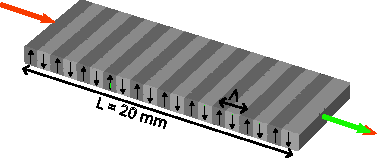
\includegraphics[height=4.5cm]{./img/PP.pdf}
\end{figure}


%$\chi^{(2)} \to \chie := \frac2\pi \chi^{(2)}$, $\Delta k \to \dke := \Delta k - k_\mathsc{\chi}$


\end{frame}

\begin{frame}
\begin{align*}
\left|\A_2(L)\right| \approx \frac{\chie\omega}{2 cn_2} \A_1^2 L\ \left|\operatorname{sinc}\left( \frac{\dke L}{2} \right)\right|
\end{align*}
\begin{figure}
\centering
% This file was created with tikzplotlib v0.10.1.
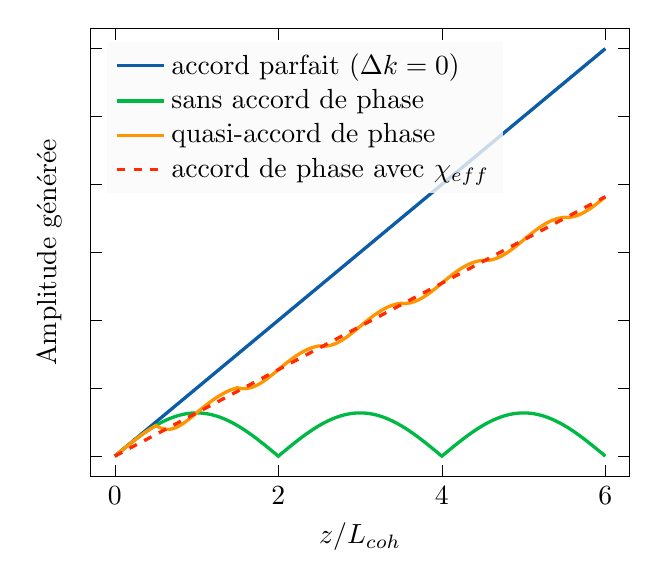
\begin{tikzpicture}

\definecolor{darkgray176}{RGB}{176,176,176}
\definecolor{darkorange2551490}{RGB}{255,149,0}
\definecolor{limegreen018569}{RGB}{0,185,69}
\definecolor{orangered255440}{RGB}{255,44,0}
\definecolor{teal1293165}{RGB}{12,93,165}

\begin{axis}[
legend cell align={left},
legend style={
	fill=black!2,
  fill opacity=0.8,
  draw opacity=1,
  text opacity=1,
  at={(0.03,0.97)},
  anchor=north west,
  draw=none
},
tick pos=both,
x grid style={darkgray176},
xlabel={\(\displaystyle z/L_\text{coh}\)},
xmin=-0.3, xmax=6.3,
xtick style={color=black},
xtick={-2,0,2,4,6,8},
xticklabels={
  \(\displaystyle {\ensuremath{-}2}\),
  \(\displaystyle {0}\),
  \(\displaystyle {2}\),
  \(\displaystyle {4}\),
  \(\displaystyle {6}\),
  \(\displaystyle {8}\)
},
y grid style={darkgray176},
ylabel={Amplitude générée},
ymin=-0.3, ymax=6.3,
ytick style={color=black},
ytick={-1,0,1,2,3,4,5,6,7},
yticklabels={
%  \(\displaystyle {\ensuremath{-}1}\),
%  \(\displaystyle {0}\),
%  \(\displaystyle {1}\),
%  \(\displaystyle {2}\),
%  \(\displaystyle {3}\),
%  \(\displaystyle {4}\),
%  \(\displaystyle {5}\),
%  \(\displaystyle {6}\),
%  \(\displaystyle {7}\)
}
]
\addplot [very thick, teal1293165]
table {%
0 0
0.00600600600600601 0.00600600600600601
0.012012012012012 0.012012012012012
0.018018018018018 0.018018018018018
0.024024024024024 0.024024024024024
0.03003003003003 0.03003003003003
0.036036036036036 0.036036036036036
0.042042042042042 0.042042042042042
0.048048048048048 0.048048048048048
0.0540540540540541 0.0540540540540541
0.0600600600600601 0.0600600600600601
0.0660660660660661 0.0660660660660661
0.0720720720720721 0.0720720720720721
0.0780780780780781 0.0780780780780781
0.0840840840840841 0.0840840840840841
0.0900900900900901 0.0900900900900901
0.0960960960960961 0.0960960960960961
0.102102102102102 0.102102102102102
0.108108108108108 0.108108108108108
0.114114114114114 0.114114114114114
0.12012012012012 0.12012012012012
0.126126126126126 0.126126126126126
0.132132132132132 0.132132132132132
0.138138138138138 0.138138138138138
0.144144144144144 0.144144144144144
0.15015015015015 0.15015015015015
0.156156156156156 0.156156156156156
0.162162162162162 0.162162162162162
0.168168168168168 0.168168168168168
0.174174174174174 0.174174174174174
0.18018018018018 0.18018018018018
0.186186186186186 0.186186186186186
0.192192192192192 0.192192192192192
0.198198198198198 0.198198198198198
0.204204204204204 0.204204204204204
0.21021021021021 0.21021021021021
0.216216216216216 0.216216216216216
0.222222222222222 0.222222222222222
0.228228228228228 0.228228228228228
0.234234234234234 0.234234234234234
0.24024024024024 0.24024024024024
0.246246246246246 0.246246246246246
0.252252252252252 0.252252252252252
0.258258258258258 0.258258258258258
0.264264264264264 0.264264264264264
0.27027027027027 0.27027027027027
0.276276276276276 0.276276276276276
0.282282282282282 0.282282282282282
0.288288288288288 0.288288288288288
0.294294294294294 0.294294294294294
0.3003003003003 0.3003003003003
0.306306306306306 0.306306306306306
0.312312312312312 0.312312312312312
0.318318318318318 0.318318318318318
0.324324324324324 0.324324324324324
0.33033033033033 0.33033033033033
0.336336336336336 0.336336336336336
0.342342342342342 0.342342342342342
0.348348348348348 0.348348348348348
0.354354354354354 0.354354354354354
0.36036036036036 0.36036036036036
0.366366366366366 0.366366366366366
0.372372372372372 0.372372372372372
0.378378378378378 0.378378378378378
0.384384384384384 0.384384384384384
0.39039039039039 0.39039039039039
0.396396396396396 0.396396396396396
0.402402402402402 0.402402402402402
0.408408408408408 0.408408408408408
0.414414414414414 0.414414414414414
0.42042042042042 0.42042042042042
0.426426426426426 0.426426426426426
0.432432432432432 0.432432432432432
0.438438438438438 0.438438438438438
0.444444444444444 0.444444444444444
0.45045045045045 0.45045045045045
0.456456456456456 0.456456456456456
0.462462462462462 0.462462462462462
0.468468468468468 0.468468468468468
0.474474474474474 0.474474474474474
0.48048048048048 0.48048048048048
0.486486486486486 0.486486486486486
0.492492492492492 0.492492492492492
0.498498498498498 0.498498498498498
0.504504504504504 0.504504504504504
0.510510510510511 0.510510510510511
0.516516516516517 0.516516516516517
0.522522522522523 0.522522522522523
0.528528528528528 0.528528528528528
0.534534534534534 0.534534534534534
0.540540540540541 0.540540540540541
0.546546546546547 0.546546546546547
0.552552552552553 0.552552552552553
0.558558558558559 0.558558558558559
0.564564564564565 0.564564564564565
0.570570570570571 0.570570570570571
0.576576576576577 0.576576576576577
0.582582582582583 0.582582582582583
0.588588588588589 0.588588588588589
0.594594594594595 0.594594594594595
0.600600600600601 0.600600600600601
0.606606606606607 0.606606606606607
0.612612612612613 0.612612612612613
0.618618618618619 0.618618618618619
0.624624624624625 0.624624624624625
0.630630630630631 0.630630630630631
0.636636636636637 0.636636636636637
0.642642642642643 0.642642642642643
0.648648648648649 0.648648648648649
0.654654654654655 0.654654654654655
0.660660660660661 0.660660660660661
0.666666666666667 0.666666666666667
0.672672672672673 0.672672672672673
0.678678678678679 0.678678678678679
0.684684684684685 0.684684684684685
0.690690690690691 0.690690690690691
0.696696696696697 0.696696696696697
0.702702702702703 0.702702702702703
0.708708708708709 0.708708708708709
0.714714714714715 0.714714714714715
0.720720720720721 0.720720720720721
0.726726726726727 0.726726726726727
0.732732732732733 0.732732732732733
0.738738738738739 0.738738738738739
0.744744744744745 0.744744744744745
0.750750750750751 0.750750750750751
0.756756756756757 0.756756756756757
0.762762762762763 0.762762762762763
0.768768768768769 0.768768768768769
0.774774774774775 0.774774774774775
0.780780780780781 0.780780780780781
0.786786786786787 0.786786786786787
0.792792792792793 0.792792792792793
0.798798798798799 0.798798798798799
0.804804804804805 0.804804804804805
0.810810810810811 0.810810810810811
0.816816816816817 0.816816816816817
0.822822822822823 0.822822822822823
0.828828828828829 0.828828828828829
0.834834834834835 0.834834834834835
0.840840840840841 0.840840840840841
0.846846846846847 0.846846846846847
0.852852852852853 0.852852852852853
0.858858858858859 0.858858858858859
0.864864864864865 0.864864864864865
0.870870870870871 0.870870870870871
0.876876876876877 0.876876876876877
0.882882882882883 0.882882882882883
0.888888888888889 0.888888888888889
0.894894894894895 0.894894894894895
0.900900900900901 0.900900900900901
0.906906906906907 0.906906906906907
0.912912912912913 0.912912912912913
0.918918918918919 0.918918918918919
0.924924924924925 0.924924924924925
0.930930930930931 0.930930930930931
0.936936936936937 0.936936936936937
0.942942942942943 0.942942942942943
0.948948948948949 0.948948948948949
0.954954954954955 0.954954954954955
0.960960960960961 0.960960960960961
0.966966966966967 0.966966966966967
0.972972972972973 0.972972972972973
0.978978978978979 0.978978978978979
0.984984984984985 0.984984984984985
0.990990990990991 0.990990990990991
0.996996996996997 0.996996996996997
1.003003003003 1.003003003003
1.00900900900901 1.00900900900901
1.01501501501502 1.01501501501502
1.02102102102102 1.02102102102102
1.02702702702703 1.02702702702703
1.03303303303303 1.03303303303303
1.03903903903904 1.03903903903904
1.04504504504505 1.04504504504505
1.05105105105105 1.05105105105105
1.05705705705706 1.05705705705706
1.06306306306306 1.06306306306306
1.06906906906907 1.06906906906907
1.07507507507508 1.07507507507508
1.08108108108108 1.08108108108108
1.08708708708709 1.08708708708709
1.09309309309309 1.09309309309309
1.0990990990991 1.0990990990991
1.10510510510511 1.10510510510511
1.11111111111111 1.11111111111111
1.11711711711712 1.11711711711712
1.12312312312312 1.12312312312312
1.12912912912913 1.12912912912913
1.13513513513514 1.13513513513514
1.14114114114114 1.14114114114114
1.14714714714715 1.14714714714715
1.15315315315315 1.15315315315315
1.15915915915916 1.15915915915916
1.16516516516517 1.16516516516517
1.17117117117117 1.17117117117117
1.17717717717718 1.17717717717718
1.18318318318318 1.18318318318318
1.18918918918919 1.18918918918919
1.1951951951952 1.1951951951952
1.2012012012012 1.2012012012012
1.20720720720721 1.20720720720721
1.21321321321321 1.21321321321321
1.21921921921922 1.21921921921922
1.22522522522523 1.22522522522523
1.23123123123123 1.23123123123123
1.23723723723724 1.23723723723724
1.24324324324324 1.24324324324324
1.24924924924925 1.24924924924925
1.25525525525526 1.25525525525526
1.26126126126126 1.26126126126126
1.26726726726727 1.26726726726727
1.27327327327327 1.27327327327327
1.27927927927928 1.27927927927928
1.28528528528529 1.28528528528529
1.29129129129129 1.29129129129129
1.2972972972973 1.2972972972973
1.3033033033033 1.3033033033033
1.30930930930931 1.30930930930931
1.31531531531532 1.31531531531532
1.32132132132132 1.32132132132132
1.32732732732733 1.32732732732733
1.33333333333333 1.33333333333333
1.33933933933934 1.33933933933934
1.34534534534535 1.34534534534535
1.35135135135135 1.35135135135135
1.35735735735736 1.35735735735736
1.36336336336336 1.36336336336336
1.36936936936937 1.36936936936937
1.37537537537538 1.37537537537538
1.38138138138138 1.38138138138138
1.38738738738739 1.38738738738739
1.39339339339339 1.39339339339339
1.3993993993994 1.3993993993994
1.40540540540541 1.40540540540541
1.41141141141141 1.41141141141141
1.41741741741742 1.41741741741742
1.42342342342342 1.42342342342342
1.42942942942943 1.42942942942943
1.43543543543544 1.43543543543544
1.44144144144144 1.44144144144144
1.44744744744745 1.44744744744745
1.45345345345345 1.45345345345345
1.45945945945946 1.45945945945946
1.46546546546547 1.46546546546547
1.47147147147147 1.47147147147147
1.47747747747748 1.47747747747748
1.48348348348348 1.48348348348348
1.48948948948949 1.48948948948949
1.4954954954955 1.4954954954955
1.5015015015015 1.5015015015015
1.50750750750751 1.50750750750751
1.51351351351351 1.51351351351351
1.51951951951952 1.51951951951952
1.52552552552553 1.52552552552553
1.53153153153153 1.53153153153153
1.53753753753754 1.53753753753754
1.54354354354354 1.54354354354354
1.54954954954955 1.54954954954955
1.55555555555556 1.55555555555556
1.56156156156156 1.56156156156156
1.56756756756757 1.56756756756757
1.57357357357357 1.57357357357357
1.57957957957958 1.57957957957958
1.58558558558559 1.58558558558559
1.59159159159159 1.59159159159159
1.5975975975976 1.5975975975976
1.6036036036036 1.6036036036036
1.60960960960961 1.60960960960961
1.61561561561562 1.61561561561562
1.62162162162162 1.62162162162162
1.62762762762763 1.62762762762763
1.63363363363363 1.63363363363363
1.63963963963964 1.63963963963964
1.64564564564565 1.64564564564565
1.65165165165165 1.65165165165165
1.65765765765766 1.65765765765766
1.66366366366366 1.66366366366366
1.66966966966967 1.66966966966967
1.67567567567568 1.67567567567568
1.68168168168168 1.68168168168168
1.68768768768769 1.68768768768769
1.69369369369369 1.69369369369369
1.6996996996997 1.6996996996997
1.70570570570571 1.70570570570571
1.71171171171171 1.71171171171171
1.71771771771772 1.71771771771772
1.72372372372372 1.72372372372372
1.72972972972973 1.72972972972973
1.73573573573574 1.73573573573574
1.74174174174174 1.74174174174174
1.74774774774775 1.74774774774775
1.75375375375375 1.75375375375375
1.75975975975976 1.75975975975976
1.76576576576577 1.76576576576577
1.77177177177177 1.77177177177177
1.77777777777778 1.77777777777778
1.78378378378378 1.78378378378378
1.78978978978979 1.78978978978979
1.7957957957958 1.7957957957958
1.8018018018018 1.8018018018018
1.80780780780781 1.80780780780781
1.81381381381381 1.81381381381381
1.81981981981982 1.81981981981982
1.82582582582583 1.82582582582583
1.83183183183183 1.83183183183183
1.83783783783784 1.83783783783784
1.84384384384384 1.84384384384384
1.84984984984985 1.84984984984985
1.85585585585586 1.85585585585586
1.86186186186186 1.86186186186186
1.86786786786787 1.86786786786787
1.87387387387387 1.87387387387387
1.87987987987988 1.87987987987988
1.88588588588589 1.88588588588589
1.89189189189189 1.89189189189189
1.8978978978979 1.8978978978979
1.9039039039039 1.9039039039039
1.90990990990991 1.90990990990991
1.91591591591592 1.91591591591592
1.92192192192192 1.92192192192192
1.92792792792793 1.92792792792793
1.93393393393393 1.93393393393393
1.93993993993994 1.93993993993994
1.94594594594595 1.94594594594595
1.95195195195195 1.95195195195195
1.95795795795796 1.95795795795796
1.96396396396396 1.96396396396396
1.96996996996997 1.96996996996997
1.97597597597598 1.97597597597598
1.98198198198198 1.98198198198198
1.98798798798799 1.98798798798799
1.99399399399399 1.99399399399399
2 2
2.00600600600601 2.00600600600601
2.01201201201201 2.01201201201201
2.01801801801802 2.01801801801802
2.02402402402402 2.02402402402402
2.03003003003003 2.03003003003003
2.03603603603604 2.03603603603604
2.04204204204204 2.04204204204204
2.04804804804805 2.04804804804805
2.05405405405405 2.05405405405405
2.06006006006006 2.06006006006006
2.06606606606607 2.06606606606607
2.07207207207207 2.07207207207207
2.07807807807808 2.07807807807808
2.08408408408408 2.08408408408408
2.09009009009009 2.09009009009009
2.0960960960961 2.0960960960961
2.1021021021021 2.1021021021021
2.10810810810811 2.10810810810811
2.11411411411411 2.11411411411411
2.12012012012012 2.12012012012012
2.12612612612613 2.12612612612613
2.13213213213213 2.13213213213213
2.13813813813814 2.13813813813814
2.14414414414414 2.14414414414414
2.15015015015015 2.15015015015015
2.15615615615616 2.15615615615616
2.16216216216216 2.16216216216216
2.16816816816817 2.16816816816817
2.17417417417417 2.17417417417417
2.18018018018018 2.18018018018018
2.18618618618619 2.18618618618619
2.19219219219219 2.19219219219219
2.1981981981982 2.1981981981982
2.2042042042042 2.2042042042042
2.21021021021021 2.21021021021021
2.21621621621622 2.21621621621622
2.22222222222222 2.22222222222222
2.22822822822823 2.22822822822823
2.23423423423423 2.23423423423423
2.24024024024024 2.24024024024024
2.24624624624625 2.24624624624625
2.25225225225225 2.25225225225225
2.25825825825826 2.25825825825826
2.26426426426426 2.26426426426426
2.27027027027027 2.27027027027027
2.27627627627628 2.27627627627628
2.28228228228228 2.28228228228228
2.28828828828829 2.28828828828829
2.29429429429429 2.29429429429429
2.3003003003003 2.3003003003003
2.30630630630631 2.30630630630631
2.31231231231231 2.31231231231231
2.31831831831832 2.31831831831832
2.32432432432432 2.32432432432432
2.33033033033033 2.33033033033033
2.33633633633634 2.33633633633634
2.34234234234234 2.34234234234234
2.34834834834835 2.34834834834835
2.35435435435435 2.35435435435435
2.36036036036036 2.36036036036036
2.36636636636637 2.36636636636637
2.37237237237237 2.37237237237237
2.37837837837838 2.37837837837838
2.38438438438438 2.38438438438438
2.39039039039039 2.39039039039039
2.3963963963964 2.3963963963964
2.4024024024024 2.4024024024024
2.40840840840841 2.40840840840841
2.41441441441441 2.41441441441441
2.42042042042042 2.42042042042042
2.42642642642643 2.42642642642643
2.43243243243243 2.43243243243243
2.43843843843844 2.43843843843844
2.44444444444444 2.44444444444444
2.45045045045045 2.45045045045045
2.45645645645646 2.45645645645646
2.46246246246246 2.46246246246246
2.46846846846847 2.46846846846847
2.47447447447447 2.47447447447447
2.48048048048048 2.48048048048048
2.48648648648649 2.48648648648649
2.49249249249249 2.49249249249249
2.4984984984985 2.4984984984985
2.5045045045045 2.5045045045045
2.51051051051051 2.51051051051051
2.51651651651652 2.51651651651652
2.52252252252252 2.52252252252252
2.52852852852853 2.52852852852853
2.53453453453453 2.53453453453453
2.54054054054054 2.54054054054054
2.54654654654655 2.54654654654655
2.55255255255255 2.55255255255255
2.55855855855856 2.55855855855856
2.56456456456456 2.56456456456456
2.57057057057057 2.57057057057057
2.57657657657658 2.57657657657658
2.58258258258258 2.58258258258258
2.58858858858859 2.58858858858859
2.59459459459459 2.59459459459459
2.6006006006006 2.6006006006006
2.60660660660661 2.60660660660661
2.61261261261261 2.61261261261261
2.61861861861862 2.61861861861862
2.62462462462462 2.62462462462462
2.63063063063063 2.63063063063063
2.63663663663664 2.63663663663664
2.64264264264264 2.64264264264264
2.64864864864865 2.64864864864865
2.65465465465465 2.65465465465465
2.66066066066066 2.66066066066066
2.66666666666667 2.66666666666667
2.67267267267267 2.67267267267267
2.67867867867868 2.67867867867868
2.68468468468468 2.68468468468468
2.69069069069069 2.69069069069069
2.6966966966967 2.6966966966967
2.7027027027027 2.7027027027027
2.70870870870871 2.70870870870871
2.71471471471471 2.71471471471471
2.72072072072072 2.72072072072072
2.72672672672673 2.72672672672673
2.73273273273273 2.73273273273273
2.73873873873874 2.73873873873874
2.74474474474474 2.74474474474474
2.75075075075075 2.75075075075075
2.75675675675676 2.75675675675676
2.76276276276276 2.76276276276276
2.76876876876877 2.76876876876877
2.77477477477477 2.77477477477477
2.78078078078078 2.78078078078078
2.78678678678679 2.78678678678679
2.79279279279279 2.79279279279279
2.7987987987988 2.7987987987988
2.8048048048048 2.8048048048048
2.81081081081081 2.81081081081081
2.81681681681682 2.81681681681682
2.82282282282282 2.82282282282282
2.82882882882883 2.82882882882883
2.83483483483483 2.83483483483483
2.84084084084084 2.84084084084084
2.84684684684685 2.84684684684685
2.85285285285285 2.85285285285285
2.85885885885886 2.85885885885886
2.86486486486486 2.86486486486486
2.87087087087087 2.87087087087087
2.87687687687688 2.87687687687688
2.88288288288288 2.88288288288288
2.88888888888889 2.88888888888889
2.89489489489489 2.89489489489489
2.9009009009009 2.9009009009009
2.90690690690691 2.90690690690691
2.91291291291291 2.91291291291291
2.91891891891892 2.91891891891892
2.92492492492492 2.92492492492492
2.93093093093093 2.93093093093093
2.93693693693694 2.93693693693694
2.94294294294294 2.94294294294294
2.94894894894895 2.94894894894895
2.95495495495495 2.95495495495495
2.96096096096096 2.96096096096096
2.96696696696697 2.96696696696697
2.97297297297297 2.97297297297297
2.97897897897898 2.97897897897898
2.98498498498498 2.98498498498498
2.99099099099099 2.99099099099099
2.996996996997 2.996996996997
3.003003003003 3.003003003003
3.00900900900901 3.00900900900901
3.01501501501502 3.01501501501502
3.02102102102102 3.02102102102102
3.02702702702703 3.02702702702703
3.03303303303303 3.03303303303303
3.03903903903904 3.03903903903904
3.04504504504505 3.04504504504505
3.05105105105105 3.05105105105105
3.05705705705706 3.05705705705706
3.06306306306306 3.06306306306306
3.06906906906907 3.06906906906907
3.07507507507508 3.07507507507508
3.08108108108108 3.08108108108108
3.08708708708709 3.08708708708709
3.09309309309309 3.09309309309309
3.0990990990991 3.0990990990991
3.10510510510511 3.10510510510511
3.11111111111111 3.11111111111111
3.11711711711712 3.11711711711712
3.12312312312312 3.12312312312312
3.12912912912913 3.12912912912913
3.13513513513514 3.13513513513514
3.14114114114114 3.14114114114114
3.14714714714715 3.14714714714715
3.15315315315315 3.15315315315315
3.15915915915916 3.15915915915916
3.16516516516517 3.16516516516517
3.17117117117117 3.17117117117117
3.17717717717718 3.17717717717718
3.18318318318318 3.18318318318318
3.18918918918919 3.18918918918919
3.1951951951952 3.1951951951952
3.2012012012012 3.2012012012012
3.20720720720721 3.20720720720721
3.21321321321321 3.21321321321321
3.21921921921922 3.21921921921922
3.22522522522523 3.22522522522523
3.23123123123123 3.23123123123123
3.23723723723724 3.23723723723724
3.24324324324324 3.24324324324324
3.24924924924925 3.24924924924925
3.25525525525526 3.25525525525526
3.26126126126126 3.26126126126126
3.26726726726727 3.26726726726727
3.27327327327327 3.27327327327327
3.27927927927928 3.27927927927928
3.28528528528529 3.28528528528529
3.29129129129129 3.29129129129129
3.2972972972973 3.2972972972973
3.3033033033033 3.3033033033033
3.30930930930931 3.30930930930931
3.31531531531532 3.31531531531532
3.32132132132132 3.32132132132132
3.32732732732733 3.32732732732733
3.33333333333333 3.33333333333333
3.33933933933934 3.33933933933934
3.34534534534535 3.34534534534535
3.35135135135135 3.35135135135135
3.35735735735736 3.35735735735736
3.36336336336336 3.36336336336336
3.36936936936937 3.36936936936937
3.37537537537538 3.37537537537538
3.38138138138138 3.38138138138138
3.38738738738739 3.38738738738739
3.39339339339339 3.39339339339339
3.3993993993994 3.3993993993994
3.40540540540541 3.40540540540541
3.41141141141141 3.41141141141141
3.41741741741742 3.41741741741742
3.42342342342342 3.42342342342342
3.42942942942943 3.42942942942943
3.43543543543544 3.43543543543544
3.44144144144144 3.44144144144144
3.44744744744745 3.44744744744745
3.45345345345345 3.45345345345345
3.45945945945946 3.45945945945946
3.46546546546547 3.46546546546547
3.47147147147147 3.47147147147147
3.47747747747748 3.47747747747748
3.48348348348348 3.48348348348348
3.48948948948949 3.48948948948949
3.4954954954955 3.4954954954955
3.5015015015015 3.5015015015015
3.50750750750751 3.50750750750751
3.51351351351351 3.51351351351351
3.51951951951952 3.51951951951952
3.52552552552553 3.52552552552553
3.53153153153153 3.53153153153153
3.53753753753754 3.53753753753754
3.54354354354354 3.54354354354354
3.54954954954955 3.54954954954955
3.55555555555556 3.55555555555556
3.56156156156156 3.56156156156156
3.56756756756757 3.56756756756757
3.57357357357357 3.57357357357357
3.57957957957958 3.57957957957958
3.58558558558559 3.58558558558559
3.59159159159159 3.59159159159159
3.5975975975976 3.5975975975976
3.6036036036036 3.6036036036036
3.60960960960961 3.60960960960961
3.61561561561562 3.61561561561562
3.62162162162162 3.62162162162162
3.62762762762763 3.62762762762763
3.63363363363363 3.63363363363363
3.63963963963964 3.63963963963964
3.64564564564565 3.64564564564565
3.65165165165165 3.65165165165165
3.65765765765766 3.65765765765766
3.66366366366366 3.66366366366366
3.66966966966967 3.66966966966967
3.67567567567568 3.67567567567568
3.68168168168168 3.68168168168168
3.68768768768769 3.68768768768769
3.69369369369369 3.69369369369369
3.6996996996997 3.6996996996997
3.70570570570571 3.70570570570571
3.71171171171171 3.71171171171171
3.71771771771772 3.71771771771772
3.72372372372372 3.72372372372372
3.72972972972973 3.72972972972973
3.73573573573574 3.73573573573574
3.74174174174174 3.74174174174174
3.74774774774775 3.74774774774775
3.75375375375375 3.75375375375375
3.75975975975976 3.75975975975976
3.76576576576577 3.76576576576577
3.77177177177177 3.77177177177177
3.77777777777778 3.77777777777778
3.78378378378378 3.78378378378378
3.78978978978979 3.78978978978979
3.7957957957958 3.7957957957958
3.8018018018018 3.8018018018018
3.80780780780781 3.80780780780781
3.81381381381381 3.81381381381381
3.81981981981982 3.81981981981982
3.82582582582583 3.82582582582583
3.83183183183183 3.83183183183183
3.83783783783784 3.83783783783784
3.84384384384384 3.84384384384384
3.84984984984985 3.84984984984985
3.85585585585586 3.85585585585586
3.86186186186186 3.86186186186186
3.86786786786787 3.86786786786787
3.87387387387387 3.87387387387387
3.87987987987988 3.87987987987988
3.88588588588589 3.88588588588589
3.89189189189189 3.89189189189189
3.8978978978979 3.8978978978979
3.9039039039039 3.9039039039039
3.90990990990991 3.90990990990991
3.91591591591592 3.91591591591592
3.92192192192192 3.92192192192192
3.92792792792793 3.92792792792793
3.93393393393393 3.93393393393393
3.93993993993994 3.93993993993994
3.94594594594595 3.94594594594595
3.95195195195195 3.95195195195195
3.95795795795796 3.95795795795796
3.96396396396396 3.96396396396396
3.96996996996997 3.96996996996997
3.97597597597598 3.97597597597598
3.98198198198198 3.98198198198198
3.98798798798799 3.98798798798799
3.99399399399399 3.99399399399399
4 4
4.00600600600601 4.00600600600601
4.01201201201201 4.01201201201201
4.01801801801802 4.01801801801802
4.02402402402402 4.02402402402402
4.03003003003003 4.03003003003003
4.03603603603604 4.03603603603604
4.04204204204204 4.04204204204204
4.04804804804805 4.04804804804805
4.05405405405405 4.05405405405405
4.06006006006006 4.06006006006006
4.06606606606607 4.06606606606607
4.07207207207207 4.07207207207207
4.07807807807808 4.07807807807808
4.08408408408408 4.08408408408408
4.09009009009009 4.09009009009009
4.0960960960961 4.0960960960961
4.1021021021021 4.1021021021021
4.10810810810811 4.10810810810811
4.11411411411411 4.11411411411411
4.12012012012012 4.12012012012012
4.12612612612613 4.12612612612613
4.13213213213213 4.13213213213213
4.13813813813814 4.13813813813814
4.14414414414414 4.14414414414414
4.15015015015015 4.15015015015015
4.15615615615616 4.15615615615616
4.16216216216216 4.16216216216216
4.16816816816817 4.16816816816817
4.17417417417417 4.17417417417417
4.18018018018018 4.18018018018018
4.18618618618619 4.18618618618619
4.19219219219219 4.19219219219219
4.1981981981982 4.1981981981982
4.2042042042042 4.2042042042042
4.21021021021021 4.21021021021021
4.21621621621622 4.21621621621622
4.22222222222222 4.22222222222222
4.22822822822823 4.22822822822823
4.23423423423423 4.23423423423423
4.24024024024024 4.24024024024024
4.24624624624625 4.24624624624625
4.25225225225225 4.25225225225225
4.25825825825826 4.25825825825826
4.26426426426426 4.26426426426426
4.27027027027027 4.27027027027027
4.27627627627628 4.27627627627628
4.28228228228228 4.28228228228228
4.28828828828829 4.28828828828829
4.29429429429429 4.29429429429429
4.3003003003003 4.3003003003003
4.30630630630631 4.30630630630631
4.31231231231231 4.31231231231231
4.31831831831832 4.31831831831832
4.32432432432432 4.32432432432432
4.33033033033033 4.33033033033033
4.33633633633634 4.33633633633634
4.34234234234234 4.34234234234234
4.34834834834835 4.34834834834835
4.35435435435435 4.35435435435435
4.36036036036036 4.36036036036036
4.36636636636637 4.36636636636637
4.37237237237237 4.37237237237237
4.37837837837838 4.37837837837838
4.38438438438438 4.38438438438438
4.39039039039039 4.39039039039039
4.3963963963964 4.3963963963964
4.4024024024024 4.4024024024024
4.40840840840841 4.40840840840841
4.41441441441441 4.41441441441441
4.42042042042042 4.42042042042042
4.42642642642643 4.42642642642643
4.43243243243243 4.43243243243243
4.43843843843844 4.43843843843844
4.44444444444444 4.44444444444444
4.45045045045045 4.45045045045045
4.45645645645646 4.45645645645646
4.46246246246246 4.46246246246246
4.46846846846847 4.46846846846847
4.47447447447447 4.47447447447447
4.48048048048048 4.48048048048048
4.48648648648649 4.48648648648649
4.49249249249249 4.49249249249249
4.4984984984985 4.4984984984985
4.5045045045045 4.5045045045045
4.51051051051051 4.51051051051051
4.51651651651652 4.51651651651652
4.52252252252252 4.52252252252252
4.52852852852853 4.52852852852853
4.53453453453453 4.53453453453453
4.54054054054054 4.54054054054054
4.54654654654655 4.54654654654655
4.55255255255255 4.55255255255255
4.55855855855856 4.55855855855856
4.56456456456456 4.56456456456456
4.57057057057057 4.57057057057057
4.57657657657658 4.57657657657658
4.58258258258258 4.58258258258258
4.58858858858859 4.58858858858859
4.59459459459459 4.59459459459459
4.6006006006006 4.6006006006006
4.60660660660661 4.60660660660661
4.61261261261261 4.61261261261261
4.61861861861862 4.61861861861862
4.62462462462462 4.62462462462462
4.63063063063063 4.63063063063063
4.63663663663664 4.63663663663664
4.64264264264264 4.64264264264264
4.64864864864865 4.64864864864865
4.65465465465465 4.65465465465465
4.66066066066066 4.66066066066066
4.66666666666667 4.66666666666667
4.67267267267267 4.67267267267267
4.67867867867868 4.67867867867868
4.68468468468468 4.68468468468468
4.69069069069069 4.69069069069069
4.6966966966967 4.6966966966967
4.7027027027027 4.7027027027027
4.70870870870871 4.70870870870871
4.71471471471471 4.71471471471471
4.72072072072072 4.72072072072072
4.72672672672673 4.72672672672673
4.73273273273273 4.73273273273273
4.73873873873874 4.73873873873874
4.74474474474474 4.74474474474474
4.75075075075075 4.75075075075075
4.75675675675676 4.75675675675676
4.76276276276276 4.76276276276276
4.76876876876877 4.76876876876877
4.77477477477477 4.77477477477477
4.78078078078078 4.78078078078078
4.78678678678679 4.78678678678679
4.79279279279279 4.79279279279279
4.7987987987988 4.7987987987988
4.8048048048048 4.8048048048048
4.81081081081081 4.81081081081081
4.81681681681682 4.81681681681682
4.82282282282282 4.82282282282282
4.82882882882883 4.82882882882883
4.83483483483483 4.83483483483483
4.84084084084084 4.84084084084084
4.84684684684685 4.84684684684685
4.85285285285285 4.85285285285285
4.85885885885886 4.85885885885886
4.86486486486486 4.86486486486486
4.87087087087087 4.87087087087087
4.87687687687688 4.87687687687688
4.88288288288288 4.88288288288288
4.88888888888889 4.88888888888889
4.89489489489489 4.89489489489489
4.9009009009009 4.9009009009009
4.90690690690691 4.90690690690691
4.91291291291291 4.91291291291291
4.91891891891892 4.91891891891892
4.92492492492492 4.92492492492492
4.93093093093093 4.93093093093093
4.93693693693694 4.93693693693694
4.94294294294294 4.94294294294294
4.94894894894895 4.94894894894895
4.95495495495495 4.95495495495495
4.96096096096096 4.96096096096096
4.96696696696697 4.96696696696697
4.97297297297297 4.97297297297297
4.97897897897898 4.97897897897898
4.98498498498498 4.98498498498498
4.99099099099099 4.99099099099099
4.996996996997 4.996996996997
5.003003003003 5.003003003003
5.00900900900901 5.00900900900901
5.01501501501502 5.01501501501502
5.02102102102102 5.02102102102102
5.02702702702703 5.02702702702703
5.03303303303303 5.03303303303303
5.03903903903904 5.03903903903904
5.04504504504505 5.04504504504505
5.05105105105105 5.05105105105105
5.05705705705706 5.05705705705706
5.06306306306306 5.06306306306306
5.06906906906907 5.06906906906907
5.07507507507508 5.07507507507508
5.08108108108108 5.08108108108108
5.08708708708709 5.08708708708709
5.09309309309309 5.09309309309309
5.0990990990991 5.0990990990991
5.10510510510511 5.10510510510511
5.11111111111111 5.11111111111111
5.11711711711712 5.11711711711712
5.12312312312312 5.12312312312312
5.12912912912913 5.12912912912913
5.13513513513514 5.13513513513514
5.14114114114114 5.14114114114114
5.14714714714715 5.14714714714715
5.15315315315315 5.15315315315315
5.15915915915916 5.15915915915916
5.16516516516517 5.16516516516517
5.17117117117117 5.17117117117117
5.17717717717718 5.17717717717718
5.18318318318318 5.18318318318318
5.18918918918919 5.18918918918919
5.1951951951952 5.1951951951952
5.2012012012012 5.2012012012012
5.20720720720721 5.20720720720721
5.21321321321321 5.21321321321321
5.21921921921922 5.21921921921922
5.22522522522523 5.22522522522523
5.23123123123123 5.23123123123123
5.23723723723724 5.23723723723724
5.24324324324324 5.24324324324324
5.24924924924925 5.24924924924925
5.25525525525526 5.25525525525526
5.26126126126126 5.26126126126126
5.26726726726727 5.26726726726727
5.27327327327327 5.27327327327327
5.27927927927928 5.27927927927928
5.28528528528529 5.28528528528529
5.29129129129129 5.29129129129129
5.2972972972973 5.2972972972973
5.3033033033033 5.3033033033033
5.30930930930931 5.30930930930931
5.31531531531532 5.31531531531532
5.32132132132132 5.32132132132132
5.32732732732733 5.32732732732733
5.33333333333333 5.33333333333333
5.33933933933934 5.33933933933934
5.34534534534535 5.34534534534535
5.35135135135135 5.35135135135135
5.35735735735736 5.35735735735736
5.36336336336336 5.36336336336336
5.36936936936937 5.36936936936937
5.37537537537538 5.37537537537538
5.38138138138138 5.38138138138138
5.38738738738739 5.38738738738739
5.39339339339339 5.39339339339339
5.3993993993994 5.3993993993994
5.40540540540541 5.40540540540541
5.41141141141141 5.41141141141141
5.41741741741742 5.41741741741742
5.42342342342342 5.42342342342342
5.42942942942943 5.42942942942943
5.43543543543544 5.43543543543544
5.44144144144144 5.44144144144144
5.44744744744745 5.44744744744745
5.45345345345345 5.45345345345345
5.45945945945946 5.45945945945946
5.46546546546547 5.46546546546547
5.47147147147147 5.47147147147147
5.47747747747748 5.47747747747748
5.48348348348348 5.48348348348348
5.48948948948949 5.48948948948949
5.4954954954955 5.4954954954955
5.5015015015015 5.5015015015015
5.50750750750751 5.50750750750751
5.51351351351351 5.51351351351351
5.51951951951952 5.51951951951952
5.52552552552553 5.52552552552553
5.53153153153153 5.53153153153153
5.53753753753754 5.53753753753754
5.54354354354354 5.54354354354354
5.54954954954955 5.54954954954955
5.55555555555556 5.55555555555556
5.56156156156156 5.56156156156156
5.56756756756757 5.56756756756757
5.57357357357357 5.57357357357357
5.57957957957958 5.57957957957958
5.58558558558559 5.58558558558559
5.59159159159159 5.59159159159159
5.5975975975976 5.5975975975976
5.6036036036036 5.6036036036036
5.60960960960961 5.60960960960961
5.61561561561562 5.61561561561562
5.62162162162162 5.62162162162162
5.62762762762763 5.62762762762763
5.63363363363363 5.63363363363363
5.63963963963964 5.63963963963964
5.64564564564565 5.64564564564565
5.65165165165165 5.65165165165165
5.65765765765766 5.65765765765766
5.66366366366366 5.66366366366366
5.66966966966967 5.66966966966967
5.67567567567568 5.67567567567568
5.68168168168168 5.68168168168168
5.68768768768769 5.68768768768769
5.69369369369369 5.69369369369369
5.6996996996997 5.6996996996997
5.70570570570571 5.70570570570571
5.71171171171171 5.71171171171171
5.71771771771772 5.71771771771772
5.72372372372372 5.72372372372372
5.72972972972973 5.72972972972973
5.73573573573574 5.73573573573574
5.74174174174174 5.74174174174174
5.74774774774775 5.74774774774775
5.75375375375375 5.75375375375375
5.75975975975976 5.75975975975976
5.76576576576577 5.76576576576577
5.77177177177177 5.77177177177177
5.77777777777778 5.77777777777778
5.78378378378378 5.78378378378378
5.78978978978979 5.78978978978979
5.7957957957958 5.7957957957958
5.8018018018018 5.8018018018018
5.80780780780781 5.80780780780781
5.81381381381381 5.81381381381381
5.81981981981982 5.81981981981982
5.82582582582583 5.82582582582583
5.83183183183183 5.83183183183183
5.83783783783784 5.83783783783784
5.84384384384384 5.84384384384384
5.84984984984985 5.84984984984985
5.85585585585586 5.85585585585586
5.86186186186186 5.86186186186186
5.86786786786787 5.86786786786787
5.87387387387387 5.87387387387387
5.87987987987988 5.87987987987988
5.88588588588589 5.88588588588589
5.89189189189189 5.89189189189189
5.8978978978979 5.8978978978979
5.9039039039039 5.9039039039039
5.90990990990991 5.90990990990991
5.91591591591592 5.91591591591592
5.92192192192192 5.92192192192192
5.92792792792793 5.92792792792793
5.93393393393393 5.93393393393393
5.93993993993994 5.93993993993994
5.94594594594595 5.94594594594595
5.95195195195195 5.95195195195195
5.95795795795796 5.95795795795796
5.96396396396396 5.96396396396396
5.96996996996997 5.96996996996997
5.97597597597598 5.97597597597598
5.98198198198198 5.98198198198198
5.98798798798799 5.98798798798799
5.99399399399399 5.99399399399399
6 6
};
\addlegendentry{accord parfait ($\Delta k = 0$)}
\addplot [very thick, limegreen018569]
table {%
0 0
0.00600600600600601 0.0060057387276301
0.012012012012012 0.0120109429222971
0.018018018018018 0.0180150780986135
0.024024024024024 0.0240176098663381
0.03003003003003 0.0300180039779391
0.036036036036036 0.0360157263761442
0.042042042042042 0.0420102432414732
0.048048048048048 0.0480010210397504
0.0540540540540541 0.0539875265695907
0.0600600600600601 0.0599692270098568
0.0660660660660661 0.0659455899670822
0.0720720720720721 0.0719160835228561
0.0780780780780781 0.077880176281166
0.0840840840840841 0.0838373374156943
0.0900900900900901 0.0897870367170633
0.0960960960960961 0.0957287446400263
0.102102102102102 0.101661932350599
0.108108108108108 0.107586071773126
0.114114114114114 0.113500635637286
0.12012012012012 0.119405097525015
0.126126126126126 0.125298931917363
0.132132132132132 0.131181614241268
0.138138138138138 0.137052620916241
0.144144144144144 0.142911429400971
0.15015015015015 0.148757518239829
0.156156156156156 0.154590367109283
0.162162162162162 0.160409456864207
0.168168168168168 0.166214269584087
0.174174174174174 0.172004288619118
0.18018018018018 0.177778998636187
0.186186186186186 0.183537885664742
0.192192192192192 0.189280437142533
0.198198198198198 0.195006141961236
0.204204204204204 0.200714490511943
0.21021021021021 0.206404974730515
0.216216216216216 0.212077088142807
0.222222222222222 0.217730325909744
0.228228228228228 0.223364184872252
0.234234234234234 0.228978163596042
0.24024024024024 0.234571762416241
0.246246246246246 0.240144483481862
0.252252252252252 0.245695830800116
0.258258258258258 0.251225310280556
0.264264264264264 0.256732429779054
0.27027027027027 0.262216699141603
0.276276276276276 0.267677630247942
0.282282282282282 0.273114737055002
0.288288288288288 0.278527535640164
0.294294294294294 0.283915544244331
0.3003003003003 0.289278283314806
0.306306306306306 0.294615275547974
0.312312312312312 0.299926045931784
0.318318318318318 0.305210121788026
0.324324324324324 0.310467032814402
0.33033033033033 0.315696311126385
0.336336336336336 0.320897491298861
0.342342342342342 0.326070110407555
0.348348348348348 0.331213708070231
0.354354354354354 0.33632782648767
0.36036036036036 0.341412010484415
0.366366366366366 0.346465807549283
0.372372372372372 0.351488767875641
0.378378378378378 0.356480444401438
0.384384384384384 0.361440392848999
0.39039039039039 0.366368171764563
0.396396396396396 0.37126334255758
0.402402402402402 0.37612546953974
0.408408408408408 0.380954119963756
0.414414414414414 0.385748864061878
0.42042042042042 0.390509275084144
0.426426426426426 0.395234929336365
0.432432432432432 0.399925406217831
0.438438438438438 0.404580288258747
0.444444444444444 0.409199161157395
0.45045045045045 0.413781613816998
0.456456456456456 0.41832723838232
0.462462462462462 0.42283563027596
0.468468468468468 0.42730638823436
0.474474474474474 0.431739114343525
0.48048048048048 0.436133414074434
0.486486486486486 0.440488896318154
0.492492492492492 0.444805173420656
0.498498498498498 0.44908186121731
0.504504504504504 0.453318579067081
0.510510510510511 0.45751494988641
0.516516516516517 0.461670600182769
0.522522522522523 0.46578516008791
0.528528528528528 0.469858263390782
0.534534534534534 0.473889547570122
0.540540540540541 0.477878653826726
0.546546546546547 0.481825227115382
0.552552552552553 0.485728916176467
0.558558558558559 0.489589373567215
0.564564564564565 0.493406255692637
0.570570570570571 0.497179222836104
0.576576576576577 0.500907939189585
0.582582582582583 0.50459207288353
0.588588588588589 0.508231296016413
0.594594594594595 0.511825284683912
0.600600600600601 0.515373719007742
0.606606606606607 0.518876283164121
0.612612612612613 0.522332665411882
0.618618618618619 0.52574255812022
0.624624624624625 0.52910565779607
0.630630630630631 0.53242166511112
0.636636636636637 0.535690284928453
0.642642642642643 0.538911226328813
0.648648648648649 0.542084202636502
0.654654654654655 0.54520893144489
0.660660660660661 0.548285134641554
0.666666666666667 0.551312538433031
0.672672672672673 0.554290873369184
0.678678678678679 0.557219874367187
0.684684684684685 0.560099280735115
0.690690690690691 0.562928836195151
0.696696696696697 0.565708288906392
0.702702702702703 0.568437391487264
0.708708708708709 0.571115901037543
0.714714714714715 0.57374357915997
0.720720720720721 0.576320191981472
0.726726726726727 0.578845510173977
0.732732732732733 0.581319308974824
0.738738738738739 0.583741368206768
0.744744744744745 0.586111472297579
0.750750750750751 0.588429410299225
0.756756756756757 0.590694975906648
0.762762762762763 0.592907967476131
0.768768768768769 0.595068188043235
0.774774774774775 0.597175445340341
0.780780780780781 0.599229551813753
0.786786786786787 0.601230324640396
0.792792792792793 0.603177585744089
0.798798798798799 0.60507116181139
0.804804804804805 0.606910884307023
0.810810810810811 0.608696589488881
0.816816816816817 0.610428118422598
0.822822822822823 0.612105316995693
0.828828828828829 0.613728035931288
0.834834834834835 0.615296130801397
0.840840840840841 0.616809462039774
0.846846846846847 0.618267894954342
0.852852852852853 0.619671299739175
0.858858858858859 0.621019551486058
0.864864864864865 0.622312530195596
0.870870870870871 0.623550120787902
0.876876876876877 0.624732213112835
0.882882882882883 0.625858701959805
0.888888888888889 0.626929487067138
0.894894894894895 0.627944473130999
0.900900900900901 0.628903569813872
0.906906906906907 0.629806691752605
0.912912912912913 0.630653758566006
0.918918918918919 0.631444694861993
0.924924924924925 0.632179430244312
0.930930930930931 0.632857899318794
0.936936936936937 0.633480041699183
0.942942942942943 0.634045802012505
0.948948948948949 0.634555129904
0.954954954954955 0.635007980041601
0.960960960960961 0.635404312119971
0.966966966966967 0.635744090864088
0.972972972972973 0.636027286032388
0.978978978978979 0.636253872419453
0.984984984984985 0.636423829858256
0.990990990990991 0.636537143221957
0.996996996996997 0.636593802425247
1.003003003003 0.636593802425247
1.00900900900901 0.636537143221957
1.01501501501502 0.636423829858256
1.02102102102102 0.636253872419453
1.02702702702703 0.636027286032388
1.03303303303303 0.635744090864088
1.03903903903904 0.635404312119971
1.04504504504505 0.635007980041601
1.05105105105105 0.634555129904
1.05705705705706 0.634045802012505
1.06306306306306 0.633480041699183
1.06906906906907 0.632857899318794
1.07507507507508 0.632179430244312
1.08108108108108 0.631444694861993
1.08708708708709 0.630653758566006
1.09309309309309 0.629806691752605
1.0990990990991 0.628903569813872
1.10510510510511 0.627944473130999
1.11111111111111 0.626929487067138
1.11711711711712 0.625858701959805
1.12312312312312 0.624732213112835
1.12912912912913 0.623550120787902
1.13513513513514 0.622312530195596
1.14114114114114 0.621019551486058
1.14714714714715 0.619671299739175
1.15315315315315 0.618267894954342
1.15915915915916 0.616809462039774
1.16516516516517 0.615296130801397
1.17117117117117 0.613728035931288
1.17717717717718 0.612105316995692
1.18318318318318 0.610428118422597
1.18918918918919 0.608696589488881
1.1951951951952 0.606910884307022
1.2012012012012 0.605071161811389
1.20720720720721 0.603177585744089
1.21321321321321 0.601230324640396
1.21921921921922 0.599229551813752
1.22522522522523 0.59717544534034
1.23123123123123 0.595068188043235
1.23723723723724 0.59290796747613
1.24324324324324 0.590694975906648
1.24924924924925 0.588429410299224
1.25525525525526 0.586111472297579
1.26126126126126 0.583741368206768
1.26726726726727 0.581319308974823
1.27327327327327 0.578845510173977
1.27927927927928 0.576320191981472
1.28528528528529 0.57374357915997
1.29129129129129 0.571115901037543
1.2972972972973 0.568437391487264
1.3033033033033 0.565708288906391
1.30930930930931 0.562928836195151
1.31531531531532 0.560099280735115
1.32132132132132 0.557219874367186
1.32732732732733 0.554290873369183
1.33333333333333 0.55131253843303
1.33933933933934 0.548285134641553
1.34534534534535 0.545208931444889
1.35135135135135 0.542084202636501
1.35735735735736 0.538911226328813
1.36336336336336 0.535690284928452
1.36936936936937 0.53242166511112
1.37537537537538 0.529105657796069
1.38138138138138 0.525742558120219
1.38738738738739 0.522332665411881
1.39339339339339 0.51887628316412
1.3993993993994 0.515373719007741
1.40540540540541 0.511825284683912
1.41141141141141 0.508231296016413
1.41741741741742 0.50459207288353
1.42342342342342 0.500907939189585
1.42942942942943 0.497179222836104
1.43543543543544 0.493406255692636
1.44144144144144 0.489589373567214
1.44744744744745 0.485728916176467
1.45345345345345 0.481825227115382
1.45945945945946 0.477878653826726
1.46546546546547 0.473889547570121
1.47147147147147 0.469858263390781
1.47747747747748 0.46578516008791
1.48348348348348 0.461670600182769
1.48948948948949 0.45751494988641
1.4954954954955 0.453318579067081
1.5015015015015 0.44908186121731
1.50750750750751 0.444805173420656
1.51351351351351 0.440488896318154
1.51951951951952 0.436133414074433
1.52552552552553 0.431739114343525
1.53153153153153 0.42730638823436
1.53753753753754 0.422835630275959
1.54354354354354 0.41832723838232
1.54954954954955 0.413781613816998
1.55555555555556 0.409199161157394
1.56156156156156 0.404580288258747
1.56756756756757 0.39992540621783
1.57357357357357 0.395234929336365
1.57957957957958 0.390509275084144
1.58558558558559 0.385748864061877
1.59159159159159 0.380954119963756
1.5975975975976 0.37612546953974
1.6036036036036 0.37126334255758
1.60960960960961 0.366368171764563
1.61561561561562 0.361440392848998
1.62162162162162 0.356480444401438
1.62762762762763 0.351488767875641
1.63363363363363 0.346465807549283
1.63963963963964 0.341412010484415
1.64564564564565 0.33632782648767
1.65165165165165 0.33121370807023
1.65765765765766 0.326070110407555
1.66366366366366 0.320897491298861
1.66966966966967 0.315696311126385
1.67567567567568 0.310467032814402
1.68168168168168 0.305210121788026
1.68768768768769 0.299926045931784
1.69369369369369 0.294615275547974
1.6996996996997 0.289278283314806
1.70570570570571 0.283915544244331
1.71171171171171 0.278527535640164
1.71771771771772 0.273114737055002
1.72372372372372 0.267677630247942
1.72972972972973 0.262216699141603
1.73573573573574 0.256732429779054
1.74174174174174 0.251225310280556
1.74774774774775 0.245695830800116
1.75375375375375 0.240144483481862
1.75975975975976 0.23457176241624
1.76576576576577 0.228978163596042
1.77177177177177 0.223364184872251
1.77777777777778 0.217730325909744
1.78378378378378 0.212077088142807
1.78978978978979 0.206404974730515
1.7957957957958 0.200714490511943
1.8018018018018 0.195006141961236
1.80780780780781 0.189280437142533
1.81381381381381 0.183537885664742
1.81981981981982 0.177778998636187
1.82582582582583 0.172004288619118
1.83183183183183 0.166214269584087
1.83783783783784 0.160409456864207
1.84384384384384 0.154590367109283
1.84984984984985 0.148757518239829
1.85585585585586 0.142911429400971
1.86186186186186 0.137052620916241
1.86786786786787 0.131181614241268
1.87387387387387 0.125298931917363
1.87987987987988 0.119405097525015
1.88588588588589 0.113500635637286
1.89189189189189 0.107586071773126
1.8978978978979 0.101661932350599
1.9039039039039 0.0957287446400264
1.90990990990991 0.0897870367170633
1.91591591591592 0.0838373374156944
1.92192192192192 0.0778801762811661
1.92792792792793 0.0719160835228561
1.93393393393393 0.0659455899670824
1.93993993993994 0.0599692270098569
1.94594594594595 0.0539875265695909
1.95195195195195 0.0480010210397505
1.95795795795796 0.0420102432414733
1.96396396396396 0.0360157263761444
1.96996996996997 0.0300180039779392
1.97597597597598 0.0240176098663383
1.98198198198198 0.0180150780986136
1.98798798798799 0.0120109429222972
1.99399399399399 0.00600573872763032
2 5.82315660888803e-16
2.00600600600601 0.00600573872763003
2.01201201201201 0.0120109429222972
2.01801801801802 0.0180150780986131
2.02402402402402 0.0240176098663378
2.03003003003003 0.0300180039779389
2.03603603603604 0.0360157263761441
2.04204204204204 0.0420102432414732
2.04804804804805 0.04800102103975
2.05405405405405 0.0539875265695904
2.06006006006006 0.0599692270098566
2.06606606606607 0.0659455899670821
2.07207207207207 0.071916083522856
2.07807807807808 0.0778801762811656
2.08408408408408 0.0838373374156939
2.09009009009009 0.089787036717063
2.0960960960961 0.0957287446400261
2.1021021021021 0.101661932350599
2.10810810810811 0.107586071773126
2.11411411411411 0.113500635637285
2.12012012012012 0.119405097525014
2.12612612612613 0.125298931917363
2.13213213213213 0.131181614241268
2.13813813813814 0.137052620916241
2.14414414414414 0.14291142940097
2.15015015015015 0.148757518239828
2.15615615615616 0.154590367109283
2.16216216216216 0.160409456864207
2.16816816816817 0.166214269584087
2.17417417417417 0.172004288619118
2.18018018018018 0.177778998636187
2.18618618618619 0.183537885664742
2.19219219219219 0.189280437142533
2.1981981981982 0.195006141961236
2.2042042042042 0.200714490511942
2.21021021021021 0.206404974730515
2.21621621621622 0.212077088142807
2.22222222222222 0.217730325909744
2.22822822822823 0.223364184872251
2.23423423423423 0.228978163596041
2.24024024024024 0.23457176241624
2.24624624624625 0.240144483481862
2.25225225225225 0.245695830800116
2.25825825825826 0.251225310280556
2.26426426426426 0.256732429779054
2.27027027027027 0.262216699141603
2.27627627627628 0.267677630247942
2.28228228228228 0.273114737055002
2.28828828828829 0.278527535640164
2.29429429429429 0.28391554424433
2.3003003003003 0.289278283314805
2.30630630630631 0.294615275547973
2.31231231231231 0.299926045931783
2.31831831831832 0.305210121788026
2.32432432432432 0.310467032814402
2.33033033033033 0.315696311126385
2.33633633633634 0.320897491298861
2.34234234234234 0.326070110407555
2.34834834834835 0.33121370807023
2.35435435435435 0.336327826487669
2.36036036036036 0.341412010484414
2.36636636636637 0.346465807549283
2.37237237237237 0.35148876787564
2.37837837837838 0.356480444401438
2.38438438438438 0.361440392848998
2.39039039039039 0.366368171764563
2.3963963963964 0.37126334255758
2.4024024024024 0.37612546953974
2.40840840840841 0.380954119963756
2.41441441441441 0.385748864061877
2.42042042042042 0.390509275084144
2.42642642642643 0.395234929336365
2.43243243243243 0.39992540621783
2.43843843843844 0.404580288258747
2.44444444444444 0.409199161157394
2.45045045045045 0.413781613816998
2.45645645645646 0.41832723838232
2.46246246246246 0.422835630275959
2.46846846846847 0.42730638823436
2.47447447447447 0.431739114343525
2.48048048048048 0.436133414074433
2.48648648648649 0.440488896318154
2.49249249249249 0.444805173420656
2.4984984984985 0.449081861217309
2.5045045045045 0.453318579067081
2.51051051051051 0.457514949886409
2.51651651651652 0.461670600182769
2.52252252252252 0.46578516008791
2.52852852852853 0.469858263390781
2.53453453453453 0.473889547570121
2.54054054054054 0.477878653826726
2.54654654654655 0.481825227115381
2.55255255255255 0.485728916176467
2.55855855855856 0.489589373567214
2.56456456456456 0.493406255692636
2.57057057057057 0.497179222836104
2.57657657657658 0.500907939189585
2.58258258258258 0.50459207288353
2.58858858858859 0.508231296016413
2.59459459459459 0.511825284683912
2.6006006006006 0.515373719007741
2.60660660660661 0.51887628316412
2.61261261261261 0.522332665411881
2.61861861861862 0.525742558120219
2.62462462462462 0.529105657796069
2.63063063063063 0.532421665111119
2.63663663663664 0.535690284928452
2.64264264264264 0.538911226328813
2.64864864864865 0.542084202636501
2.65465465465465 0.545208931444889
2.66066066066066 0.548285134641553
2.66666666666667 0.55131253843303
2.67267267267267 0.554290873369183
2.67867867867868 0.557219874367186
2.68468468468468 0.560099280735115
2.69069069069069 0.562928836195151
2.6966966966967 0.565708288906391
2.7027027027027 0.568437391487264
2.70870870870871 0.571115901037542
2.71471471471471 0.57374357915997
2.72072072072072 0.576320191981472
2.72672672672673 0.578845510173976
2.73273273273273 0.581319308974823
2.73873873873874 0.583741368206768
2.74474474474474 0.586111472297579
2.75075075075075 0.588429410299224
2.75675675675676 0.590694975906648
2.76276276276276 0.59290796747613
2.76876876876877 0.595068188043235
2.77477477477477 0.59717544534034
2.78078078078078 0.599229551813752
2.78678678678679 0.601230324640396
2.79279279279279 0.603177585744089
2.7987987987988 0.605071161811389
2.8048048048048 0.606910884307022
2.81081081081081 0.608696589488881
2.81681681681682 0.610428118422597
2.82282282282282 0.612105316995692
2.82882882882883 0.613728035931288
2.83483483483483 0.615296130801396
2.84084084084084 0.616809462039774
2.84684684684685 0.618267894954341
2.85285285285285 0.619671299739175
2.85885885885886 0.621019551486057
2.86486486486486 0.622312530195596
2.87087087087087 0.623550120787902
2.87687687687688 0.624732213112835
2.88288288288288 0.625858701959805
2.88888888888889 0.626929487067138
2.89489489489489 0.627944473130998
2.9009009009009 0.628903569813872
2.90690690690691 0.629806691752605
2.91291291291291 0.630653758566005
2.91891891891892 0.631444694861993
2.92492492492492 0.632179430244311
2.93093093093093 0.632857899318794
2.93693693693694 0.633480041699183
2.94294294294294 0.634045802012505
2.94894894894895 0.634555129904
2.95495495495495 0.635007980041601
2.96096096096096 0.635404312119971
2.96696696696697 0.635744090864088
2.97297297297297 0.636027286032388
2.97897897897898 0.636253872419453
2.98498498498498 0.636423829858256
2.99099099099099 0.636537143221956
2.996996996997 0.636593802425246
3.003003003003 0.636593802425246
3.00900900900901 0.636537143221956
3.01501501501502 0.636423829858256
3.02102102102102 0.636253872419453
3.02702702702703 0.636027286032388
3.03303303303303 0.635744090864088
3.03903903903904 0.635404312119971
3.04504504504505 0.635007980041601
3.05105105105105 0.634555129904
3.05705705705706 0.634045802012505
3.06306306306306 0.633480041699183
3.06906906906907 0.632857899318794
3.07507507507508 0.632179430244311
3.08108108108108 0.631444694861993
3.08708708708709 0.630653758566006
3.09309309309309 0.629806691752605
3.0990990990991 0.628903569813872
3.10510510510511 0.627944473130998
3.11111111111111 0.626929487067138
3.11711711711712 0.625858701959805
3.12312312312312 0.624732213112835
3.12912912912913 0.623550120787902
3.13513513513514 0.622312530195596
3.14114114114114 0.621019551486057
3.14714714714715 0.619671299739175
3.15315315315315 0.618267894954341
3.15915915915916 0.616809462039774
3.16516516516517 0.615296130801396
3.17117117117117 0.613728035931288
3.17717717717718 0.612105316995692
3.18318318318318 0.610428118422597
3.18918918918919 0.608696589488881
3.1951951951952 0.606910884307022
3.2012012012012 0.605071161811389
3.20720720720721 0.603177585744089
3.21321321321321 0.601230324640396
3.21921921921922 0.599229551813752
3.22522522522523 0.59717544534034
3.23123123123123 0.595068188043235
3.23723723723724 0.59290796747613
3.24324324324324 0.590694975906648
3.24924924924925 0.588429410299224
3.25525525525526 0.586111472297579
3.26126126126126 0.583741368206768
3.26726726726727 0.581319308974823
3.27327327327327 0.578845510173977
3.27927927927928 0.576320191981472
3.28528528528529 0.57374357915997
3.29129129129129 0.571115901037543
3.2972972972973 0.568437391487264
3.3033033033033 0.565708288906391
3.30930930930931 0.562928836195151
3.31531531531532 0.560099280735115
3.32132132132132 0.557219874367186
3.32732732732733 0.554290873369184
3.33333333333333 0.55131253843303
3.33933933933934 0.548285134641554
3.34534534534535 0.545208931444889
3.35135135135135 0.542084202636501
3.35735735735736 0.538911226328813
3.36336336336336 0.535690284928452
3.36936936936937 0.53242166511112
3.37537537537538 0.52910565779607
3.38138138138138 0.525742558120219
3.38738738738739 0.522332665411881
3.39339339339339 0.51887628316412
3.3993993993994 0.515373719007742
3.40540540540541 0.511825284683912
3.41141141141141 0.508231296016413
3.41741741741742 0.50459207288353
3.42342342342342 0.500907939189585
3.42942942942943 0.497179222836104
3.43543543543544 0.493406255692636
3.44144144144144 0.489589373567214
3.44744744744745 0.485728916176467
3.45345345345345 0.481825227115381
3.45945945945946 0.477878653826726
3.46546546546547 0.473889547570121
3.47147147147147 0.469858263390781
3.47747747747748 0.46578516008791
3.48348348348348 0.461670600182769
3.48948948948949 0.457514949886409
3.4954954954955 0.453318579067081
3.5015015015015 0.449081861217309
3.50750750750751 0.444805173420656
3.51351351351351 0.440488896318154
3.51951951951952 0.436133414074433
3.52552552552553 0.431739114343525
3.53153153153153 0.42730638823436
3.53753753753754 0.422835630275959
3.54354354354354 0.41832723838232
3.54954954954955 0.413781613816998
3.55555555555556 0.409199161157395
3.56156156156156 0.404580288258747
3.56756756756757 0.39992540621783
3.57357357357357 0.395234929336365
3.57957957957958 0.390509275084144
3.58558558558559 0.385748864061878
3.59159159159159 0.380954119963756
3.5975975975976 0.37612546953974
3.6036036036036 0.37126334255758
3.60960960960961 0.366368171764563
3.61561561561562 0.361440392848999
3.62162162162162 0.356480444401438
3.62762762762763 0.351488767875641
3.63363363363363 0.346465807549283
3.63963963963964 0.341412010484415
3.64564564564565 0.33632782648767
3.65165165165165 0.331213708070231
3.65765765765766 0.326070110407555
3.66366366366366 0.320897491298861
3.66966966966967 0.315696311126385
3.67567567567568 0.310467032814402
3.68168168168168 0.305210121788026
3.68768768768769 0.299926045931784
3.69369369369369 0.294615275547974
3.6996996996997 0.289278283314805
3.70570570570571 0.283915544244331
3.71171171171171 0.278527535640164
3.71771771771772 0.273114737055002
3.72372372372372 0.267677630247942
3.72972972972973 0.262216699141603
3.73573573573574 0.256732429779054
3.74174174174174 0.251225310280556
3.74774774774775 0.245695830800116
3.75375375375375 0.240144483481862
3.75975975975976 0.23457176241624
3.76576576576577 0.228978163596041
3.77177177177177 0.223364184872252
3.77777777777778 0.217730325909744
3.78378378378378 0.212077088142807
3.78978978978979 0.206404974730515
3.7957957957958 0.200714490511943
3.8018018018018 0.195006141961237
3.80780780780781 0.189280437142533
3.81381381381381 0.183537885664742
3.81981981981982 0.177778998636187
3.82582582582583 0.172004288619118
3.83183183183183 0.166214269584087
3.83783783783784 0.160409456864207
3.84384384384384 0.154590367109283
3.84984984984985 0.148757518239829
3.85585585585586 0.142911429400971
3.86186186186186 0.137052620916241
3.86786786786787 0.131181614241268
3.87387387387387 0.125298931917363
3.87987987987988 0.119405097525015
3.88588588588589 0.113500635637286
3.89189189189189 0.107586071773126
3.8978978978979 0.101661932350599
3.9039039039039 0.0957287446400265
3.90990990990991 0.0897870367170634
3.91591591591592 0.0838373374156943
3.92192192192192 0.0778801762811664
3.92792792792793 0.0719160835228564
3.93393393393393 0.0659455899670825
3.93993993993994 0.059969227009857
3.94594594594595 0.0539875265695908
3.95195195195195 0.0480010210397508
3.95795795795796 0.0420102432414736
3.96396396396396 0.0360157263761445
3.96996996996997 0.0300180039779393
3.97597597597598 0.0240176098663382
3.98198198198198 0.0180150780986135
3.98798798798799 0.0120109429222975
3.99399399399399 0.00600573872763041
4 8.05147334781498e-16
4.00600600600601 0.0060057387276295
4.01201201201201 0.0120109429222971
4.01801801801802 0.018015078098613
4.02402402402402 0.0240176098663381
4.03003003003003 0.0300180039779388
4.03603603603604 0.0360157263761436
4.04204204204204 0.0420102432414731
4.04804804804805 0.0480010210397499
4.05405405405405 0.0539875265695907
4.06006006006006 0.0599692270098565
4.06606606606607 0.0659455899670815
4.07207207207207 0.0719160835228559
4.07807807807808 0.0778801762811655
4.08408408408408 0.0838373374156943
4.09009009009009 0.0897870367170629
4.0960960960961 0.0957287446400255
4.1021021021021 0.101661932350598
4.10810810810811 0.107586071773126
4.11411411411411 0.113500635637286
4.12012012012012 0.119405097525014
4.12612612612613 0.125298931917362
4.13213213213213 0.131181614241268
4.13813813813814 0.137052620916241
4.14414414414414 0.142911429400971
4.15015015015015 0.148757518239828
4.15615615615616 0.154590367109282
4.16216216216216 0.160409456864207
4.16816816816817 0.166214269584087
4.17417417417417 0.172004288619118
4.18018018018018 0.177778998636187
4.18618618618619 0.183537885664741
4.19219219219219 0.189280437142533
4.1981981981982 0.195006141961236
4.2042042042042 0.200714490511943
4.21021021021021 0.206404974730514
4.21621621621622 0.212077088142806
4.22222222222222 0.217730325909744
4.22822822822823 0.223364184872251
4.23423423423423 0.228978163596041
4.24024024024024 0.23457176241624
4.24624624624625 0.240144483481861
4.25225225225225 0.245695830800116
4.25825825825826 0.251225310280555
4.26426426426426 0.256732429779054
4.27027027027027 0.262216699141603
4.27627627627628 0.267677630247941
4.28228228228228 0.273114737055001
4.28828828828829 0.278527535640163
4.29429429429429 0.28391554424433
4.3003003003003 0.289278283314805
4.30630630630631 0.294615275547973
4.31231231231231 0.299926045931783
4.31831831831832 0.305210121788025
4.32432432432432 0.310467032814402
4.33033033033033 0.315696311126385
4.33633633633634 0.32089749129886
4.34234234234234 0.326070110407554
4.34834834834835 0.33121370807023
4.35435435435435 0.336327826487669
4.36036036036036 0.341412010484414
4.36636636636637 0.346465807549283
4.37237237237237 0.35148876787564
4.37837837837838 0.356480444401437
4.38438438438438 0.361440392848998
4.39039039039039 0.366368171764563
4.3963963963964 0.37126334255758
4.4024024024024 0.376125469539739
4.40840840840841 0.380954119963755
4.41441441441441 0.385748864061877
4.42042042042042 0.390509275084144
4.42642642642643 0.395234929336365
4.43243243243243 0.39992540621783
4.43843843843844 0.404580288258746
4.44444444444444 0.409199161157394
4.45045045045045 0.413781613816998
4.45645645645646 0.41832723838232
4.46246246246246 0.422835630275959
4.46846846846847 0.427306388234359
4.47447447447447 0.431739114343524
4.48048048048048 0.436133414074433
4.48648648648649 0.440488896318154
4.49249249249249 0.444805173420655
4.4984984984985 0.449081861217309
4.5045045045045 0.453318579067081
4.51051051051051 0.457514949886409
4.51651651651652 0.461670600182769
4.52252252252252 0.46578516008791
4.52852852852853 0.469858263390781
4.53453453453453 0.473889547570121
4.54054054054054 0.477878653826725
4.54654654654655 0.481825227115381
4.55255255255255 0.485728916176466
4.55855855855856 0.489589373567214
4.56456456456456 0.493406255692636
4.57057057057057 0.497179222836103
4.57657657657658 0.500907939189585
4.58258258258258 0.50459207288353
4.58858858858859 0.508231296016412
4.59459459459459 0.511825284683912
4.6006006006006 0.515373719007741
4.60660660660661 0.51887628316412
4.61261261261261 0.522332665411881
4.61861861861862 0.525742558120219
4.62462462462462 0.529105657796069
4.63063063063063 0.532421665111119
4.63663663663664 0.535690284928452
4.64264264264264 0.538911226328812
4.64864864864865 0.542084202636501
4.65465465465465 0.545208931444889
4.66066066066066 0.548285134641553
4.66666666666667 0.55131253843303
4.67267267267267 0.554290873369183
4.67867867867868 0.557219874367186
4.68468468468468 0.560099280735115
4.69069069069069 0.56292883619515
4.6966966966967 0.565708288906391
4.7027027027027 0.568437391487263
4.70870870870871 0.571115901037542
4.71471471471471 0.57374357915997
4.72072072072072 0.576320191981472
4.72672672672673 0.578845510173977
4.73273273273273 0.581319308974823
4.73873873873874 0.583741368206768
4.74474474474474 0.586111472297579
4.75075075075075 0.588429410299224
4.75675675675676 0.590694975906648
4.76276276276276 0.59290796747613
4.76876876876877 0.595068188043234
4.77477477477477 0.59717544534034
4.78078078078078 0.599229551813752
4.78678678678679 0.601230324640396
4.79279279279279 0.603177585744089
4.7987987987988 0.605071161811389
4.8048048048048 0.606910884307022
4.81081081081081 0.608696589488881
4.81681681681682 0.610428118422597
4.82282282282282 0.612105316995692
4.82882882882883 0.613728035931288
4.83483483483483 0.615296130801397
4.84084084084084 0.616809462039774
4.84684684684685 0.618267894954342
4.85285285285285 0.619671299739175
4.85885885885886 0.621019551486057
4.86486486486486 0.622312530195596
4.87087087087087 0.623550120787902
4.87687687687688 0.624732213112835
4.88288288288288 0.625858701959805
4.88888888888889 0.626929487067138
4.89489489489489 0.627944473130999
4.9009009009009 0.628903569813872
4.90690690690691 0.629806691752605
4.91291291291291 0.630653758566006
4.91891891891892 0.631444694861993
4.92492492492492 0.632179430244312
4.93093093093093 0.632857899318794
4.93693693693694 0.633480041699183
4.94294294294294 0.634045802012505
4.94894894894895 0.634555129904
4.95495495495495 0.635007980041601
4.96096096096096 0.635404312119971
4.96696696696697 0.635744090864088
4.97297297297297 0.636027286032388
4.97897897897898 0.636253872419453
4.98498498498498 0.636423829858256
4.99099099099099 0.636537143221957
4.996996996997 0.636593802425247
5.003003003003 0.636593802425247
5.00900900900901 0.636537143221957
5.01501501501502 0.636423829858256
5.02102102102102 0.636253872419453
5.02702702702703 0.636027286032388
5.03303303303303 0.635744090864088
5.03903903903904 0.635404312119971
5.04504504504505 0.635007980041601
5.05105105105105 0.634555129904
5.05705705705706 0.634045802012505
5.06306306306306 0.633480041699183
5.06906906906907 0.632857899318794
5.07507507507508 0.632179430244312
5.08108108108108 0.631444694861993
5.08708708708709 0.630653758566006
5.09309309309309 0.629806691752605
5.0990990990991 0.628903569813872
5.10510510510511 0.627944473130999
5.11111111111111 0.626929487067138
5.11711711711712 0.625858701959805
5.12312312312312 0.624732213112835
5.12912912912913 0.623550120787902
5.13513513513514 0.622312530195596
5.14114114114114 0.621019551486058
5.14714714714715 0.619671299739175
5.15315315315315 0.618267894954342
5.15915915915916 0.616809462039774
5.16516516516517 0.615296130801397
5.17117117117117 0.613728035931288
5.17717717717718 0.612105316995692
5.18318318318318 0.610428118422598
5.18918918918919 0.608696589488881
5.1951951951952 0.606910884307022
5.2012012012012 0.60507116181139
5.20720720720721 0.603177585744089
5.21321321321321 0.601230324640396
5.21921921921922 0.599229551813752
5.22522522522523 0.597175445340341
5.23123123123123 0.595068188043235
5.23723723723724 0.59290796747613
5.24324324324324 0.590694975906648
5.24924924924925 0.588429410299224
5.25525525525526 0.586111472297579
5.26126126126126 0.583741368206768
5.26726726726727 0.581319308974824
5.27327327327327 0.578845510173977
5.27927927927928 0.576320191981472
5.28528528528529 0.57374357915997
5.29129129129129 0.571115901037543
5.2972972972973 0.568437391487264
5.3033033033033 0.565708288906392
5.30930930930931 0.562928836195151
5.31531531531532 0.560099280735115
5.32132132132132 0.557219874367187
5.32732732732733 0.554290873369184
5.33333333333333 0.551312538433031
5.33933933933934 0.548285134641554
5.34534534534535 0.545208931444889
5.35135135135135 0.542084202636502
5.35735735735736 0.538911226328813
5.36336336336336 0.535690284928453
5.36936936936937 0.53242166511112
5.37537537537538 0.52910565779607
5.38138138138138 0.52574255812022
5.38738738738739 0.522332665411882
5.39339339339339 0.51887628316412
5.3993993993994 0.515373719007741
5.40540540540541 0.511825284683912
5.41141141141141 0.508231296016413
5.41741741741742 0.50459207288353
5.42342342342342 0.500907939189585
5.42942942942943 0.497179222836104
5.43543543543544 0.493406255692636
5.44144144144144 0.489589373567214
5.44744744744745 0.485728916176467
5.45345345345345 0.481825227115382
5.45945945945946 0.477878653826726
5.46546546546547 0.473889547570122
5.47147147147147 0.469858263390781
5.47747747747748 0.46578516008791
5.48348348348348 0.461670600182769
5.48948948948949 0.457514949886409
5.4954954954955 0.453318579067081
5.5015015015015 0.449081861217309
5.50750750750751 0.444805173420656
5.51351351351351 0.440488896318154
5.51951951951952 0.436133414074433
5.52552552552553 0.431739114343525
5.53153153153153 0.427306388234359
5.53753753753754 0.422835630275959
5.54354354354354 0.418327238382321
5.54954954954955 0.413781613816998
5.55555555555556 0.409199161157395
5.56156156156156 0.404580288258747
5.56756756756757 0.39992540621783
5.57357357357357 0.395234929336365
5.57957957957958 0.390509275084144
5.58558558558559 0.385748864061878
5.59159159159159 0.380954119963755
5.5975975975976 0.37612546953974
5.6036036036036 0.37126334255758
5.60960960960961 0.366368171764563
5.61561561561562 0.361440392848999
5.62162162162162 0.356480444401437
5.62762762762763 0.35148876787564
5.63363363363363 0.346465807549283
5.63963963963964 0.341412010484414
5.64564564564565 0.33632782648767
5.65165165165165 0.33121370807023
5.65765765765766 0.326070110407555
5.66366366366366 0.320897491298861
5.66966966966967 0.315696311126385
5.67567567567568 0.310467032814402
5.68168168168168 0.305210121788025
5.68768768768769 0.299926045931783
5.69369369369369 0.294615275547974
5.6996996996997 0.289278283314805
5.70570570570571 0.283915544244331
5.71171171171171 0.278527535640163
5.71771771771772 0.273114737055002
5.72372372372372 0.267677630247942
5.72972972972973 0.262216699141603
5.73573573573574 0.256732429779054
5.74174174174174 0.251225310280556
5.74774774774775 0.245695830800116
5.75375375375375 0.240144483481862
5.75975975975976 0.23457176241624
5.76576576576577 0.228978163596042
5.77177177177177 0.223364184872251
5.77777777777778 0.217730325909744
5.78378378378378 0.212077088142807
5.78978978978979 0.206404974730515
5.7957957957958 0.200714490511943
5.8018018018018 0.195006141961236
5.80780780780781 0.189280437142533
5.81381381381381 0.183537885664742
5.81981981981982 0.177778998636187
5.82582582582583 0.172004288619118
5.83183183183183 0.166214269584087
5.83783783783784 0.160409456864207
5.84384384384384 0.154590367109283
5.84984984984985 0.148757518239828
5.85585585585586 0.142911429400971
5.86186186186186 0.137052620916241
5.86786786786787 0.131181614241268
5.87387387387387 0.125298931917363
5.87987987987988 0.119405097525014
5.88588588588589 0.113500635637286
5.89189189189189 0.107586071773126
5.8978978978979 0.101661932350599
5.9039039039039 0.0957287446400257
5.90990990990991 0.089787036717063
5.91591591591592 0.0838373374156944
5.92192192192192 0.0778801762811656
5.92792792792793 0.071916083522856
5.93393393393393 0.0659455899670816
5.93993993993994 0.0599692270098566
5.94594594594595 0.0539875265695908
5.95195195195195 0.04800102103975
5.95795795795796 0.0420102432414732
5.96396396396396 0.0360157263761436
5.96996996996997 0.0300180039779389
5.97597597597598 0.0240176098663382
5.98198198198198 0.0180150780986131
5.98798798798799 0.0120109429222971
5.99399399399399 0.00600573872762956
6 4.51773577158629e-16
};
\addlegendentry{sans accord de phase}
\addplot [very thick, darkorange2551490]
table {%
0 0
0.00600600600600601 0.0060057387276301
0.012012012012012 0.0120109429222971
0.018018018018018 0.0180150780986135
0.024024024024024 0.0240176098663381
0.03003003003003 0.0300180039779391
0.036036036036036 0.0360157263761442
0.042042042042042 0.0420102432414732
0.048048048048048 0.0480010210397504
0.0540540540540541 0.0539875265695907
0.0600600600600601 0.0599692270098568
0.0660660660660661 0.0659455899670822
0.0720720720720721 0.0719160835228561
0.0780780780780781 0.077880176281166
0.0840840840840841 0.0838373374156943
0.0900900900900901 0.0897870367170633
0.0960960960960961 0.0957287446400263
0.102102102102102 0.101661932350599
0.108108108108108 0.107586071773126
0.114114114114114 0.113500635637286
0.12012012012012 0.119405097525015
0.126126126126126 0.125298931917363
0.132132132132132 0.131181614241268
0.138138138138138 0.137052620916241
0.144144144144144 0.142911429400971
0.15015015015015 0.148757518239829
0.156156156156156 0.154590367109283
0.162162162162162 0.160409456864207
0.168168168168168 0.166214269584087
0.174174174174174 0.172004288619118
0.18018018018018 0.177778998636187
0.186186186186186 0.183537885664742
0.192192192192192 0.189280437142533
0.198198198198198 0.195006141961236
0.204204204204204 0.200714490511943
0.21021021021021 0.206404974730515
0.216216216216216 0.212077088142807
0.222222222222222 0.217730325909744
0.228228228228228 0.223364184872252
0.234234234234234 0.228978163596042
0.24024024024024 0.234571762416241
0.246246246246246 0.240144483481862
0.252252252252252 0.245695830800116
0.258258258258258 0.251225310280556
0.264264264264264 0.256732429779054
0.27027027027027 0.262216699141603
0.276276276276276 0.267677630247942
0.282282282282282 0.273114737055002
0.288288288288288 0.278527535640164
0.294294294294294 0.283915544244331
0.3003003003003 0.289278283314806
0.306306306306306 0.294615275547974
0.312312312312312 0.299926045931784
0.318318318318318 0.305210121788026
0.324324324324324 0.310467032814402
0.33033033033033 0.315696311126385
0.336336336336336 0.320897491298861
0.342342342342342 0.326070110407555
0.348348348348348 0.331213708070231
0.354354354354354 0.33632782648767
0.36036036036036 0.341412010484415
0.366366366366366 0.346465807549283
0.372372372372372 0.351488767875641
0.378378378378378 0.356480444401438
0.384384384384384 0.361440392848999
0.39039039039039 0.366368171764563
0.396396396396396 0.37126334255758
0.402402402402402 0.37612546953974
0.408408408408408 0.380954119963756
0.414414414414414 0.385748864061878
0.42042042042042 0.390509275084144
0.426426426426426 0.395234929336365
0.432432432432432 0.399925406217831
0.438438438438438 0.404580288258747
0.444444444444444 0.409199161157395
0.45045045045045 0.413781613816998
0.456456456456456 0.41832723838232
0.462462462462462 0.42283563027596
0.468468468468468 0.42730638823436
0.474474474474474 0.431739114343525
0.48048048048048 0.436133414074434
0.486486486486486 0.440488896318154
0.492492492492492 0.444805173420656
0.498498498498498 0.44908186121731
0.504504504504504 0.449122210907349
0.510510510510511 0.445008809664254
0.516516516516517 0.441023272394391
0.522522522522523 0.437170534055426
0.528528528528528 0.433455525249297
0.534534534534534 0.429883156014194
0.540540540540541 0.426458298309258
0.546546546546547 0.423185767245751
0.552552552552553 0.420070301145784
0.558558558558559 0.417116540538974
0.564564564564565 0.414329006238131
0.570570570570571 0.411712076666465
0.576576576576577 0.409269964639952
0.582582582582583 0.407006693838448
0.588588588588589 0.40492607522669
0.594594594594595 0.403031683710286
0.600600600600601 0.401326835331055
0.606606606606607 0.399814565319365
0.612612612612613 0.398497607327432
0.618618618618619 0.397378374166128
0.624624624624625 0.396458940357912
0.630630630630631 0.395741026799983
0.636636636636637 0.395225987804515
0.642642642642643 0.394914800747505
0.648648648648649 0.394808058515022
0.654654654654655 0.394905964886789
0.660660660660661 0.395208332943506
0.666666666666667 0.395714586527867
0.672672672672673 0.396423764731791
0.678678678678679 0.397334529325854
0.684684684684685 0.398445174993213
0.690690690690691 0.399753642181216
0.696696696696697 0.401257532340897
0.702702702702703 0.402954125288822
0.708708708708709 0.404840398398221
0.714714714714715 0.406913047307376
0.720720720720721 0.409168507823004
0.726726726726727 0.411602978694544
0.732732732732733 0.414212444941272
0.738738738738739 0.416992701427212
0.744744744744745 0.419939376397761
0.750750750750751 0.423047954715794
0.756756756756757 0.426313800562421
0.762762762762763 0.429732179397405
0.768768768768769 0.433298279005415
0.774774774774775 0.437007229485657
0.780780780780781 0.440854122073216
0.786786786786787 0.444834026709786
0.792792792792793 0.4489420083089
0.798798798798799 0.453173141685759
0.804804804804805 0.457522525144053
0.810810810810811 0.46198529273162
0.816816816816817 0.466556625193377
0.822822822822823 0.471231759663616
0.828828828828829 0.476005998150842
0.834834834834835 0.480874714876764
0.840840840840841 0.485833362537241
0.846846846846847 0.490877477557154
0.852852852852853 0.496002684413448
0.858858858858859 0.50120469910143
0.864864864864865 0.506479331818882
0.870870870870871 0.511822488940999
0.876876876876877 0.517230174356758
0.882882882882883 0.52269849023428
0.888888888888889 0.528223637279216
0.894894894894895 0.533801914546325
0.900900900900901 0.539429718860383
0.906906906906907 0.545103543898385
0.912912912912913 0.550819978980858
0.918918918918919 0.55657570761601
0.924924924924925 0.562367505836477
0.930930930930931 0.568192240364589
0.936936936936937 0.574046866638487
0.942942942942943 0.579928426727975
0.948948948948949 0.585834047165849
0.954954954954955 0.591760936717428
0.960960960960961 0.597706384108338
0.966966966966967 0.60366775572806
0.972972972972973 0.609642493324484
0.978978978978979 0.615628111702642
0.984984984984985 0.621622196438905
0.990990990990991 0.627622401620272
0.996996996996997 0.633626447616829
1.003003003003 0.639632118894155
1.00900900900901 0.645637261871218
1.01501501501502 0.65163978282827
1.02102102102102 0.657637645868301
1.02702702702703 0.663628870934808
1.03303303303303 0.669611531887906
1.03903903903904 0.675583754640188
1.04504504504505 0.681543715353224
1.05105105105105 0.687489638695077
1.05705705705706 0.693419796158874
1.06306306306306 0.6993325044421
1.06906906906907 0.70522612388599
1.07507507507508 0.711099056974186
1.08108108108108 0.716949746889611
1.08708708708709 0.722776676128342
1.09309309309309 0.728578365169163
1.0990990990991 0.734353371197349
1.10510510510511 0.740100286881161
1.11111111111111 0.745817739199494
1.11711711711712 0.75150438831906
1.12312312312312 0.757158926519457
1.12912912912913 0.762780077164503
1.13513513513514 0.768366593718166
1.14114114114114 0.773917258803463
1.14714714714715 0.779430883302718
1.15315315315315 0.784906305497569
1.15915915915916 0.790342390247167
1.16516516516517 0.79573802820304
1.17117117117117 0.801092135059123
1.17717717717718 0.806403650835508
1.18318318318318 0.811671539194489
1.18918918918919 0.816894786787551
1.1951951951952 0.822072402631975
1.2012012012012 0.827203417515771
1.20720720720721 0.832286883429723
1.21321321321321 0.837321873025348
1.21921921921922 0.842307479097623
1.22522522522523 0.847242814091398
1.23123123123123 0.852127009630423
1.23723723723724 0.856959216067982
1.24324324324324 0.861738602058166
1.24924924924925 0.866464354146861
1.25525525525526 0.871135676381534
1.26126126126126 0.875751789939004
1.26726726726727 0.880311932770346
1.27327327327327 0.884815359262168
1.27927927927928 0.889261339913509
1.28528528528529 0.893649161027651
1.29129129129129 0.897978124418155
1.2972972972973 0.90224754712848
1.3033033033033 0.906456761164559
1.30930930930931 0.910605113239744
1.31531531531532 0.914691964531557
1.32132132132132 0.918716690449696
1.32732732732733 0.9226786804148
1.33333333333333 0.926577337647468
1.33933933933934 0.930412078967074
1.34534534534535 0.934182334599926
1.35135135135135 0.937887547996346
1.35735735735736 0.941527175656277
1.36336336336336 0.945100686963006
1.36936936936937 0.948607564024668
1.37537537537538 0.95204730152315
1.38138138138138 0.955419406570085
1.38738738738739 0.958723398569602
1.39339339339339 0.961958809087543
1.3993993993994 0.965125181726841
1.40540540540541 0.968222072008806
1.41141141141141 0.971249047260039
1.41741741741742 0.974205686504739
1.42342342342342 0.97709158036215
1.42942942942943 0.979906330948944
1.43543543543544 0.982649551786307
1.44144144144144 0.985320867711531
1.44744744744745 0.987919914793918
1.45345345345345 0.990446340254816
1.45945945945946 0.992899802391597
1.46546546546547 0.995279970505429
1.47147147147147 0.997586524832671
1.47747747747748 0.99981915647974
1.48348348348348 1.00197756736132
1.48948948948949 1.00406147014175
1.4954954954955 1.00607058817953
1.5015015015015 1.00612428226637
1.50750750750751 1.00433042978384
1.51351351351351 1.00267808135031
1.51951951951952 1.00116852720967
1.52552552552553 0.999802952708611
1.53153153153153 0.998582435610333
1.53753753753754 0.997507943623707
1.54354354354354 0.996580332161531
1.54954954954955 0.995800342340616
1.55555555555556 0.995168599235138
1.56156156156156 0.994685610393382
1.56756756756757 0.994351764626546
1.57357357357357 0.994167331076762
1.57957957957958 0.994132458569856
1.58558558558559 0.994247175256705
1.59159159159159 0.994511388545339
1.5975975975976 0.994924885324198
1.6036036036036 0.995487332475192
1.60960960960961 0.996198277673527
1.61561561561562 0.997057150469509
1.62162162162162 0.998063263645954
1.62762762762763 0.999215814843208
1.63363363363363 1.00051388844234
1.63963963963964 1.00195645769563
1.64564564564565 1.00354238709226
1.65165165165165 1.00527043494593
1.65765765765766 1.00713925619013
1.66366366366366 1.00914740536579
1.66966966966967 1.0112933397857
1.67567567567568 1.01357542285888
1.68168168168168 1.01599192755827
1.68768768768769 1.0185410400145
1.69369369369369 1.02122086321837
1.6996996996997 1.02402942081481
1.70570570570571 1.02696466097109
1.71171171171171 1.03002446030254
1.71771771771772 1.03320662783905
1.72372372372372 1.0365089090165
1.72972972972973 1.03992898967769
1.73573573573574 1.04346450006786
1.74174174174174 1.04711301881097
1.74774774774775 1.05087207685345
1.75375375375375 1.05473916136305
1.75975975975976 1.0587117195714
1.76576576576577 1.06278716254966
1.77177177177177 1.06696286890783
1.77777777777778 1.07123618840881
1.78378378378378 1.0756044454898
1.78978978978979 1.08006494268404
1.7957957957958 1.08461496393712
1.8018018018018 1.08925177781289
1.80780780780781 1.09397264058481
1.81381381381381 1.09877479920954
1.81981981981982 1.10365549418005
1.82582582582583 1.10861196225675
1.83183183183183 1.11364143907527
1.83783783783784 1.11874116163071
1.84384384384384 1.12390837063823
1.84984984984985 1.12914031277096
1.85585585585586 1.13443424277619
1.86186186186186 1.13978742547166
1.86786786786787 1.14519713762381
1.87387387387387 1.15066066971062
1.87987987987988 1.15617532757146
1.88588588588589 1.16173843394723
1.89189189189189 1.16734732991373
1.8978978978979 1.17299937621181
1.9039039039039 1.17869195447781
1.90990990990991 1.18442246837789
1.91591591591592 1.19018834465011
1.92192192192192 1.19598703405801
1.92792792792793 1.20181601225951
1.93393393393393 1.20767278059509
1.93993993993994 1.213554866799
1.94594594594595 1.21945982563739
1.95195195195195 1.22538523947714
1.95795795795796 1.23132871878905
1.96396396396396 1.2372879025891
1.96996996996997 1.24326045882129
1.97597597597598 1.24924408468563
1.98198198198198 1.25523650691449
1.98798798798799 1.26123548200076
1.99399399399399 1.2672387963808
2 1.27324426657533
2.00600600600601 1.2792497392912
2.01201201201201 1.28525309148665
2.01801801801802 1.29125223040304
2.02402402402402 1.29724509356531
2.03003003003003 1.30322964875383
2.03603603603604 1.30920389394983
2.04204204204204 1.31516585725666
2.04804804804805 1.321113596799
2.05405405405405 1.32704520060191
2.06006006006006 1.33295878645167
2.06606606606607 1.33885250174015
2.07207207207207 1.34472452329431
2.07807807807808 1.35057305719247
2.08408408408408 1.35639633856881
2.09009009009009 1.36219263140733
2.0960960960961 1.3679602283268
2.1021021021021 1.37369745035766
2.10810810810811 1.3794026467121
2.11411411411411 1.3850741945484
2.12012012012012 1.39071049873037
2.12612612612613 1.39630999158292
2.13213213213213 1.40187113264453
2.13813813813814 1.4073924084173
2.14414414414414 1.41287233211553
2.15015015015015 1.41830944341324
2.15615615615616 1.42370230819129
2.16216216216216 1.4290495182848
2.16816816816817 1.43434969123119
2.17417417417417 1.43960147001936
2.18018018018018 1.44480352284049
2.18618618618619 1.44995454284075
2.19219219219219 1.45505324787636
2.1981981981982 1.46009838027121
2.2042042042042 1.46508870657736
2.21021021021021 1.47002301733879
2.21621621621622 1.47490012685834
2.22222222222222 1.47971887296838
2.22822822822823 1.48447811680509
2.23423423423423 1.48917674258672
2.24024024024024 1.4938136573958
2.24624624624625 1.49838779096555
2.25225225225225 1.50289809547047
2.25825825825826 1.50734354532125
2.26426426426426 1.5117231369641
2.27027027027027 1.51603588868447
2.27627627627628 1.52028084041524
2.28228228228228 1.52445705354944
2.28828828828829 1.52856361075748
2.29429429429429 1.53259961580889
2.3003003003003 1.53656419339862
2.30630630630631 1.54045648897782
2.31231231231231 1.54427566858921
2.31831831831832 1.54802091870688
2.32432432432432 1.55169144608054
2.33033033033033 1.55528647758431
2.33633633633634 1.55880526006978
2.34234234234234 1.56224706022355
2.34834834834835 1.56561116442902
2.35435435435435 1.56889687863254
2.36036036036036 1.5721035282137
2.36636636636637 1.57523045785989
2.37237237237237 1.57827703144493
2.37837837837838 1.58124263191188
2.38438438438438 1.58412666115978
2.39039039039039 1.58692853993444
2.3963963963964 1.58964770772313
2.4024024024024 1.59228362265318
2.40840840840841 1.59483576139434
2.41441441441441 1.59730361906497
2.42042042042042 1.59968670914191
2.42642642642643 1.60198456337403
2.43243243243243 1.60419673169939
2.43843843843844 1.60632278216594
2.44444444444444 1.60836230085579
2.45045045045045 1.61031489181285
2.45645645645646 1.61218017697399
2.46246246246246 1.6139577961035
2.46846846846847 1.61564740673089
2.47447447447447 1.61724868409201
2.48048048048048 1.61876132107336
2.48648648648649 1.62018502815967
2.49249249249249 1.62151953338456
2.4984984984985 1.62276458228441
2.5045045045045 1.62282020476534
2.51051051051051 1.62179782040435
2.51651651651652 1.62090898351065
2.52252252252252 1.62015423054803
2.52852852852853 1.61953401784108
2.53453453453453 1.61904872091425
2.54054054054054 1.6186986339459
2.54654654654655 1.61848396933937
2.55255255255255 1.61840485741267
2.55855855855856 1.61846134620772
2.56456456456456 1.61865340142003
2.57057057057057 1.61898090644891
2.57657657657658 1.61944366256813
2.58258258258258 1.62004138921645
2.58858858858859 1.62077372440676
2.59459459459459 1.62164022525269
2.6006006006006 1.62264036861047
2.60660660660661 1.62377355183407
2.61261261261261 1.62503909364066
2.61861861861862 1.62643623508363
2.62462462462462 1.62796414062959
2.63063063063063 1.62962189933571
2.63663663663664 1.63140852612339
2.64264264264264 1.63332296314401
2.64864864864865 1.6353640812321
2.65465465465465 1.63753068144132
2.66066066066066 1.63982149665811
2.66666666666667 1.64223519328807
2.67267267267267 1.64477037300961
2.67867867867868 1.64742557458972
2.68468468468468 1.65019927575613
2.69069069069069 1.6530898951206
2.6966966966967 1.65609579414767
2.7027027027027 1.65921527916335
2.70870870870871 1.66244660339839
2.71471471471471 1.66578796906042
2.72072072072072 1.66923752942994
2.72672672672673 1.67279339097455
2.73273273273273 1.67645361547658
2.73873873873874 1.68021622216894
2.74474474474474 1.68407918987436
2.75075075075075 1.68804045914345
2.75675675675676 1.69209793438699
2.76276276276276 1.69624948599826
2.76876876876877 1.70049295246124
2.77477477477477 1.70482614244089
2.78078078078078 1.70924683685184
2.78678678678679 1.71375279090216
2.79279279279279 1.71834173610886
2.7987987987988 1.72301138228244
2.8048048048048 1.72775941947749
2.81081081081081 1.73258351990716
2.81681681681682 1.737481339819
2.82282282282282 1.74245052133035
2.82882882882883 1.74748869422137
2.83483483483483 1.75259347768417
2.84084084084084 1.75776248202674
2.84684684684685 1.76299331033042
2.85285285285285 1.76828356006003
2.85885885885886 1.77363082462579
2.86486486486486 1.77903269489666
2.87087087087087 1.78448676066435
2.87687687687688 1.78999061205808
2.88288288288288 1.79554184090973
2.88888888888889 1.80113804206958
2.89489489489489 1.80677681467274
2.9009009009009 1.81245576335661
2.90690690690691 1.81817249942972
2.91291291291291 1.82392464199257
2.91891891891892 1.82970981901103
2.92492492492492 1.83552566834295
2.93093093093093 1.84136983871892
2.93693693693694 1.84723999067787
2.94294294294294 1.85313379745858
2.94894894894895 1.85904894584792
2.95495495495495 1.86498313698699
2.96096096096096 1.87093408713613
2.96696696696697 1.8768995284
2.97297297297297 1.88287720941369
2.97897897897898 1.8888648959912
2.98498498498498 1.89486037173732
2.99099099099099 1.90086143862422
2.996996996997 1.90686591753378
3.003003003003 1.91287164876697
3.00900900900901 1.91887649252146
3.01501501501502 1.9248783293386
3.02102102102102 1.93087506052095
3.02702702702703 1.93686460852158
3.03303303303303 1.94284491730624
3.03903903903904 1.94881395268957
3.04504504504505 1.95476970264637
3.05105105105105 1.96071017759927
3.05705705705706 1.96663341068354
3.06306306306306 1.97253745799034
3.06906906906907 1.97842039878937
3.07507507507508 1.98428033573191
3.08108108108108 1.99011539503513
3.08708708708709 1.99592372664882
3.09309309309309 2.00170350440531
3.0990990990991 2.00745292615343
3.10510510510511 2.01317021387754
3.11111111111111 2.01885361380233
3.11711711711712 2.02450139648417
3.12312312312312 2.03011185688991
3.12912912912913 2.0356833144638
3.13513513513514 2.04121411318321
3.14114114114114 2.04670262160391
3.14714714714715 2.05214723289551
3.15315315315315 2.05754636486781
3.15915915915916 2.06289845998849
3.16516516516517 2.06820198539288
3.17117117117117 2.07345543288625
3.17717717717718 2.0786573189393
3.18318318318318 2.08380618467716
3.18918918918919 2.08890059586256
3.1951951951952 2.09393914287353
3.2012012012012 2.09892044067614
3.20720720720721 2.1038431287926
3.21321321321321 2.10870587126523
3.21921921921922 2.11350735661662
3.22522522522523 2.11824629780633
3.23123123123123 2.12292143218449
3.23723723723724 2.12753152144263
3.24324324324324 2.13207535156201
3.24924924924925 2.13655173275982
3.25525525525526 2.14095949943337
3.26126126126126 2.14529751010276
3.26726726726727 2.14956464735197
3.27327327327327 2.15375981776896
3.27927927927928 2.15788195188462
3.28528528528529 2.16193000411109
3.29129129129129 2.1659029526795
3.2972972972973 2.16979979957722
3.3033033033033 2.17361957048502
3.30930930930931 2.1773613147141
3.31531531531532 2.18102410514321
3.32132132132132 2.18460703815606
3.32732732732733 2.18810923357903
3.33333333333333 2.19152983461936
3.33933933933934 2.19486800780402
3.34534534534535 2.19812294291923
3.35135135135135 2.20129385295074
3.35735735735736 2.20437997402513
3.36336336336336 2.20738056535201
3.36936936936937 2.21029490916729
3.37537537537538 2.21312231067766
3.38138138138138 2.21586209800621
3.38738738738739 2.21851362213937
3.39339339339339 2.22107625687518
3.3993993993994 2.22354939877297
3.40540540540541 2.22593246710443
3.41141141141141 2.22822490380628
3.41741741741742 2.23042617343434
3.42342342342342 2.23253576311932
3.42942942942943 2.23455318252409
3.43543543543544 2.23647796380275
3.44144144144144 2.23830966156123
3.44744744744745 2.24004785281968
3.45345345345345 2.24169213697663
3.45945945945946 2.24324213577483
3.46546546546547 2.24469749326892
3.47147147147147 2.24605787579489
3.47747747747748 2.24732297194136
3.48348348348348 2.24849249252273
3.48948948948949 2.24956617055413
3.4954954954955 2.25054376122826
3.5015015015015 2.25059981991281
3.50750750750751 2.24984655183676
3.51351351351351 2.24922167128876
3.51951951951952 2.2487255078404
3.52552552552553 2.24835832339276
3.53153153153153 2.24812031188879
3.53753753753754 2.24801159909994
3.54354354354354 2.24803224248758
3.54954954954955 2.24818223113971
3.55555555555556 2.24846148578295
3.56156156156156 2.24886985886994
3.56756756756757 2.24940713474179
3.57357357357357 2.25007302986525
3.57957957957958 2.2508671931439
3.58558558558559 2.25178920630257
3.59159159159159 2.25283858434406
3.5975975975976 2.25401477607672
3.6036036036036 2.25531716471188
3.60960960960961 2.25674506852928
3.61561561561562 2.2582977416089
3.62162162162162 2.2599743746274
3.62762762762763 2.26177409571706
3.63363363363363 2.26369597138511
3.63963963963964 2.26573900749112
3.64564564564565 2.26790215028022
3.65165165165165 2.27018428746943
3.65765765765766 2.27258424938464
3.66366366366366 2.27510081014558
3.66966966966967 2.27773268889591
3.67567567567568 2.28047855107573
3.68168168168168 2.2833370097336
3.68768768768769 2.28630662687516
3.69369369369369 2.28938591484544
3.6996996996997 2.29257333774189
3.70570570570571 2.29586731285528
3.71171171171171 2.29926621213535
3.71771771771772 2.30276836367846
3.72372372372372 2.30637205323424
3.72972972972973 2.3100755257284
3.73573573573574 2.31387698679887
3.74174174174174 2.31777460434254
3.74774774774775 2.32176651006985
3.75375375375375 2.3258508010646
3.75975975975976 2.33002554134639
3.76576576576577 2.33428876343327
3.77177177177177 2.33863846990216
3.77777777777778 2.34307263494464
3.78378378378378 2.34758920591607
3.78978978978979 2.35218610487576
3.7957957957958 2.35686123011626
3.8018018018018 2.36161245767979
3.80780780780781 2.3664376428601
3.81381381381381 2.37133462168787
3.81981981981982 2.37630121239826
3.82582582582583 2.38133521687898
3.83183183183183 2.38643442209751
3.83783783783784 2.39159660150623
3.84384384384384 2.39681951642428
3.84984984984985 2.40210091739503
3.85585585585586 2.40743854551822
3.86186186186186 2.4128301337559
3.86786786786787 2.41827340821143
3.87387387387387 2.42376608938075
3.87987987987988 2.4293058933755
3.88588588588589 2.43489053311729
3.89189189189189 2.44051771950293
3.8978978978979 2.44618516254009
3.9039039039039 2.45189057245322
3.90990990990991 2.45763166075965
3.91591591591592 2.4634061413155
3.92192192192192 2.4692117313317
3.92792792792793 2.47504615235987
3.93393393393393 2.48090713124824
3.93993993993994 2.48679240106785
3.94594594594595 2.49269970200904
3.95195195195195 2.4986267822486
3.95795795795796 2.50457139878785
3.96396396396396 2.51053131826197
3.96996996996997 2.51650431772095
3.97597597597598 2.5224881853825
3.98198198198198 2.52848072135755
3.98798798798799 2.53447973834857
3.99399399399399 2.54048306232133
4 2.54648853315067
4.00600600600601 2.55249400524065
4.01201201201201 2.5584973481198
4.01801801801802 2.56449644701191
4.02402402402402 2.57048920338304
4.03003003003003 2.57647353546532
4.03603603603604 2.58244737875805
4.04204204204204 2.58840868650683
4.04804804804805 2.5943554301613
4.05405405405405 2.60028559981206
4.06006006006006 2.60619720460736
4.06606606606607 2.61208827315034
4.07207207207207 2.61795685387725
4.07807807807808 2.62380101541729
4.08408408408408 2.6296188469348
4.09009009009009 2.63540845845428
4.0960960960961 2.64116798116883
4.1021021021021 2.64689556773269
4.10810810810811 2.65258939253837
4.11411411411411 2.65824765197896
4.12012012012012 2.66386856469622
4.12612612612613 2.66945037181494
4.13213213213213 2.67499133716412
4.13813813813814 2.68048974748556
4.14414414414414 2.68594391263028
4.15015015015015 2.69135216574334
4.15615615615616 2.69671286343751
4.16216216216216 2.7020243859563
4.16816816816817 2.7072851373268
4.17417417417417 2.7124935455028
4.18018018018018 2.7176480624986
4.18618618618619 2.72274716451394
4.19219219219219 2.72778935205051
4.1981981981982 2.73277315002042
4.2042042042042 2.73769710784695
4.21021021021021 2.74255979955809
4.21621621621622 2.74735982387315
4.22222222222222 2.75209580428276
4.22822822822823 2.75676638912271
4.23423423423423 2.76137025164184
4.24024024024024 2.7659060900644
4.24624624624625 2.77037262764712
4.25225225225225 2.77476861273132
4.25825825825826 2.77909281879027
4.26426426426426 2.78334404447219
4.27027027027027 2.78752111363911
4.27627627627628 2.79162287540171
4.28228228228228 2.79564820415062
4.28828828828829 2.79959599958423
4.29429429429429 2.80346518673329
4.3003003003003 2.80725471598248
4.30630630630631 2.81096356308926
4.31231231231231 2.81459072920007
4.31831831831832 2.81813524086411
4.32432432432432 2.82159615004494
4.33033033033033 2.82497253412991
4.33633633633634 2.82826349593783
4.34234234234234 2.83146816372478
4.34834834834835 2.83458569118838
4.35435435435435 2.83761525747059
4.36036036036036 2.84055606715919
4.36636636636637 2.84340735028805
4.37237237237237 2.84616836233636
4.37837837837838 2.84883838422689
4.38438438438438 2.8514167223234
4.39039039039039 2.8539027084273
4.3963963963964 2.8562956997737
4.4024024024024 2.85859507902685
4.40840840840841 2.86080025427521
4.41441441441441 2.86291065902605
4.42042042042042 2.86492575219982
4.42642642642643 2.86684501812424
4.43243243243243 2.86866796652827
4.43843843843844 2.87039413253599
4.44444444444444 2.87202307666047
4.45045045045045 2.87355438479758
4.45645645645646 2.87498766822001
4.46246246246246 2.87632256357134
4.46846846846847 2.87755873286029
4.47447447447447 2.87869586345527
4.48048048048048 2.87973366807906
4.48648648648649 2.88067188480394
4.49249249249249 2.88151027704701
4.4984984984985 2.88224863356598
4.5045045045045 2.88230498011451
4.51051051051051 2.88179205089329
4.51651651651652 2.88140456437334
4.52252252252252 2.88114270913695
4.52852852852853 2.88100661267095
4.53453453453453 2.88099634125026
4.54054054054054 2.88111189987715
4.54654654654655 2.88135323227673
4.55255255255255 2.88172022094843
4.55855855855856 2.8822126872734
4.56456456456456 2.88283039167776
4.57057057057057 2.88357303385109
4.57657657657658 2.88444025301994
4.58258258258258 2.88543162827563
4.58858858858859 2.8865466789557
4.59459459459459 2.88778486507821
4.6006006006006 2.88914558782796
4.60660660660661 2.89062819009365
4.61261261261261 2.89223195705482
4.61861861861862 2.89395611681744
4.62462462462462 2.89579984109674
4.63063063063063 2.89776224594604
4.63663663663664 2.89984239252999
4.64264264264264 2.90203928794073
4.64864864864865 2.90435188605544
4.65465465465465 2.90677908843347
4.66066066066066 2.90931974525147
4.66666666666667 2.91197265627457
4.67267267267267 2.91473657186205
4.67867867867868 2.91761019400534
4.68468468468468 2.92059217739668
4.69069069069069 2.92368113052646
4.6966966966967 2.92687561680725
4.7027027027027 2.93017415572264
4.70870870870871 2.93357522399893
4.71471471471471 2.93707725679762
4.72072072072072 2.9406786489269
4.72672672672673 2.94437775607003
4.73273273273273 2.94817289602878
4.73873873873874 2.95206234998005
4.74474474474474 2.95604436374361
4.75075075075075 2.96011714905933
4.75675675675676 2.9642788848719
4.76276276276276 2.96852771862131
4.76876876876877 2.97286176753739
4.77477477477477 2.97727911993668
4.78078078078078 2.98177783651986
4.78678678678679 2.98635595166835
4.79279279279279 2.99101147473839
4.7987987987988 2.99574239135114
4.8048048048048 3.00054666467731
4.81081081081081 3.00542223671507
4.81681681681682 3.01036702955978
4.82282282282282 3.01537894666443
4.82882882882883 3.02045587408943
4.83483483483483 3.02559568174075
4.84084084084084 3.03079622459533
4.84684684684685 3.03605534391268
4.85285285285285 3.04137086843182
4.85885885885886 3.04674061555265
4.86486486486486 3.05216239250089
4.87087087087087 3.05763399747597
4.87687687687688 3.06315322078099
4.88288288288288 3.06871784593432
4.88888888888889 3.07432565076212
4.89489489489489 3.07997440847137
4.9009009009009 3.08566188870287
4.90690690690691 3.09138585856382
4.91291291291291 3.09714408363979
4.91891891891892 3.10293432898546
4.92492492492492 3.10875436009422
4.93093093093093 3.11460194384625
4.93693693693694 3.12047484943488
4.94294294294294 3.12637084927129
4.94894894894895 3.13228771986734
4.95495495495495 3.13822324269656
4.96096096096096 3.14417520503325
4.96696696696697 3.15014140076989
4.97297297297297 3.15611963121268
4.97897897897898 3.16210770585555
4.98498498498498 3.16810344313272
4.99099099099099 3.17410467114987
4.996996996997 3.18010922839425
5.003003003003 3.18611496442389
5.00900900900901 3.1921197405361
5.01501501501502 3.1981214304157
5.02102102102102 3.20411792076295
5.02702702702703 3.21010711190182
5.03303303303303 3.21608691836867
5.03903903903904 3.22205526948177
5.04504504504505 3.22801010989198
5.05105105105105 3.23394940011491
5.05705705705706 3.23987111704501
5.06306306306306 3.2457732544518
5.06906906906907 3.25165382345884
5.07507507507508 3.25751085300556
5.08108108108108 3.26334239029258
5.08708708708709 3.26914650121071
5.09309309309309 3.27492127075421
5.0990990990991 3.2806648034185
5.10510510510511 3.28637522358295
5.11111111111111 3.2920506758789
5.11711711711712 3.29768932554354
5.12312312312312 3.30328935875982
5.12912912912913 3.30884898298298
5.13513513513514 3.31436642725402
5.14114114114114 3.31983994250034
5.14714714714715 3.32526780182428
5.15315315315315 3.33064830077953
5.15915915915916 3.33597975763615
5.16516516516517 3.34126051363427
5.17117117117117 3.34648893322709
5.17717717717718 3.35166340431329
5.18318318318318 3.35678233845943
5.18918918918919 3.36184417111251
5.1951951951952 3.36684736180313
5.2012012012012 3.37179039433954
5.20720720720721 3.3766717769929
5.21321321321321 3.38149004267411
5.21921921921922 3.38624374910243
5.22522522522523 3.39093147896634
5.23123123123123 3.39555184007677
5.23723723723724 3.40010346551308
5.24324324324324 3.40458501376208
5.24924924924925 3.40899516885031
5.25525525525526 3.4133326404699
5.26126126126126 3.4175961640982
5.26726726726727 3.42178450111151
5.27327327327327 3.42589643889305
5.27927927927928 3.42993079093557
5.28528528528529 3.43388639693862
5.29129129129129 3.43776212290088
5.2972972972973 3.44155686120763
5.3033033033033 3.44526953071367
5.30930930930931 3.44889907682185
5.31531531531532 3.45244447155734
5.32132132132132 3.45590471363797
5.32732732732733 3.45927882854064
5.33333333333333 3.46256586856417
5.33933933933934 3.46576491288854
5.34534534534535 3.46887506763088
5.35135135135135 3.47189546589824
5.35735735735736 3.47482526783733
5.36336336336336 3.47766366068134
5.36936936936937 3.48040985879405
5.37537537537538 3.48306310371128
5.38138138138138 3.48562266417984
5.38738738738739 3.48808783619406
5.39339339339339 3.49045794303013
5.3993993993994 3.4927323352782
5.40540540540541 3.49491039087244
5.41141141141141 3.49699151511916
5.41741741741742 3.49897514072302
5.42342342342342 3.50086072781149
5.42942942942943 3.50264776395761
5.43543543543544 3.50433576420107
5.44144144144144 3.50592427106787
5.44744744744745 3.50741285458835
5.45345345345345 3.50880111231394
5.45945945945946 3.51008866933243
5.46546546546547 3.51127517828213
5.47147147147147 3.51236031936455
5.47747747747748 3.51334380035612
5.48348348348348 3.51422535661855
5.48948948948949 3.51500475110829
5.4954954954955 3.51568177438472
5.5015015015015 3.51573818026187
5.50750750750751 3.51528680567712
5.51351351351351 3.51495872566146
5.51951951951952 3.5147540915522
5.52552552552553 3.51467299776638
5.53153153153153 3.51471548172514
5.53753753753754 3.5148815238237
5.54354354354354 3.51517104744708
5.54954954954955 3.5155839190315
5.55555555555556 3.5161199481714
5.56156156156156 3.51677888777183
5.56756756756757 3.51756043424595
5.57357357357357 3.51846422775728
5.57957957957958 3.51948985250629
5.58558558558559 3.52063683706081
5.59159159159159 3.52190465472963
5.5975975975976 3.52329272397865
5.6036036036036 3.52480040888891
5.60960960960961 3.52642701965554
5.61561561561562 3.52817181312691
5.62162162162162 3.53003399338297
5.62762762762763 3.53201271235179
5.63363363363363 3.53410707046324
5.63963963963964 3.53631611733873
5.64564564564565 3.53863885251581
5.65165165165165 3.54107422620646
5.65765765765766 3.54362114008778
5.66366366366366 3.54627844812383
5.66966966966967 3.54904495741727
5.67567567567568 3.55191942908947
5.68168168168168 3.55490057918766
5.68768768768769 3.55798707961773
5.69369369369369 3.56117755910131
5.6996996996997 3.56447060415563
5.70570570570571 3.56786476009462
5.71171171171171 3.57135853205007
5.71771771771772 3.57495038601099
5.72372372372372 3.57863874988007
5.72972972972973 3.58242201454554
5.73573573573574 3.58629853496706
5.74174174174174 3.59026663127419
5.74774774774775 3.59432458987603
5.75375375375375 3.59847066458054
5.75975975975976 3.60270307772222
5.76576576576577 3.6070200212967
5.77177177177177 3.61141965810103
5.77777777777778 3.61590012287814
5.78378378378378 3.62045952346436
5.78978978978979 3.62509594193865
5.7957957957958 3.62980743577229
5.8018018018018 3.63459203897799
5.80780780780781 3.639447763257
5.81381381381381 3.64437259914338
5.81981981981982 3.64936451714419
5.82582582582583 3.65442146887456
5.83183183183183 3.65954138818678
5.83783783783784 3.66472219229226
5.84384384384384 3.66996178287566
5.84984984984985 3.67525804720016
5.85585585585586 3.68060885920312
5.86186186186186 3.68601208058136
5.86786786786787 3.69146556186526
5.87387387387387 3.69696714348115
5.87987987987988 3.70251465680107
5.88588588588589 3.70810592517961
5.89189189189189 3.71373876497699
5.8978978978979 3.71941098656806
5.9039039039039 3.72512039533667
5.90990990990991 3.73086479265492
5.91591591591592 3.73664197684696
5.92192192192192 3.74244974413702
5.92792792792793 3.74828588958117
5.93393393393393 3.75414820798279
5.93993993993994 3.76003449479124
5.94594594594595 3.76594254698373
5.95195195195195 3.77187016393001
5.95795795795796 3.77781514823998
5.96396396396396 3.7837753065938
5.96996996996997 3.7897484505547
5.97597597597598 3.79573239736424
5.98198198198198 3.80172497072009
5.98798798798799 3.80772400153623
5.99399399399399 3.81372732868573
6 3.81973279972601
};
\addlegendentry{quasi-accord de phase}
\addplot [very thick, orangered255440, dashed]
table {%
0 0
0.00600600600600601 0.00382354217638187
0.012012012012012 0.00764708435276374
0.018018018018018 0.0114706265291456
0.024024024024024 0.0152941687055275
0.03003003003003 0.0191177108819094
0.036036036036036 0.0229412530582912
0.042042042042042 0.0267647952346731
0.048048048048048 0.030588337411055
0.0540540540540541 0.0344118795874368
0.0600600600600601 0.0382354217638187
0.0660660660660661 0.0420589639402006
0.0720720720720721 0.0458825061165824
0.0780780780780781 0.0497060482929643
0.0840840840840841 0.0535295904693462
0.0900900900900901 0.0573531326457281
0.0960960960960961 0.0611766748221099
0.102102102102102 0.0650002169984918
0.108108108108108 0.0688237591748737
0.114114114114114 0.0726473013512555
0.12012012012012 0.0764708435276374
0.126126126126126 0.0802943857040193
0.132132132132132 0.0841179278804011
0.138138138138138 0.087941470056783
0.144144144144144 0.0917650122331649
0.15015015015015 0.0955885544095467
0.156156156156156 0.0994120965859286
0.162162162162162 0.10323563876231
0.168168168168168 0.107059180938692
0.174174174174174 0.110882723115074
0.18018018018018 0.114706265291456
0.186186186186186 0.118529807467838
0.192192192192192 0.12235334964422
0.198198198198198 0.126176891820602
0.204204204204204 0.130000433996984
0.21021021021021 0.133823976173365
0.216216216216216 0.137647518349747
0.222222222222222 0.141471060526129
0.228228228228228 0.145294602702511
0.234234234234234 0.149118144878893
0.24024024024024 0.152941687055275
0.246246246246246 0.156765229231657
0.252252252252252 0.160588771408038
0.258258258258258 0.16441231358442
0.264264264264264 0.168235855760802
0.27027027027027 0.172059397937184
0.276276276276276 0.175882940113566
0.282282282282282 0.179706482289948
0.288288288288288 0.18353002446633
0.294294294294294 0.187353566642712
0.3003003003003 0.191177108819093
0.306306306306306 0.195000650995475
0.312312312312312 0.198824193171857
0.318318318318318 0.202647735348239
0.324324324324324 0.206471277524621
0.33033033033033 0.210294819701003
0.336336336336336 0.214118361877385
0.342342342342342 0.217941904053767
0.348348348348348 0.221765446230149
0.354354354354354 0.22558898840653
0.36036036036036 0.229412530582912
0.366366366366366 0.233236072759294
0.372372372372372 0.237059614935676
0.378378378378378 0.240883157112058
0.384384384384384 0.24470669928844
0.39039039039039 0.248530241464822
0.396396396396396 0.252353783641204
0.402402402402402 0.256177325817585
0.408408408408408 0.260000867993967
0.414414414414414 0.263824410170349
0.42042042042042 0.267647952346731
0.426426426426426 0.271471494523113
0.432432432432432 0.275295036699495
0.438438438438438 0.279118578875877
0.444444444444444 0.282942121052258
0.45045045045045 0.28676566322864
0.456456456456456 0.290589205405022
0.462462462462462 0.294412747581404
0.468468468468468 0.298236289757786
0.474474474474474 0.302059831934168
0.48048048048048 0.30588337411055
0.486486486486486 0.309706916286932
0.492492492492492 0.313530458463313
0.498498498498498 0.317354000639695
0.504504504504504 0.321177542816077
0.510510510510511 0.325001084992459
0.516516516516517 0.328824627168841
0.522522522522523 0.332648169345223
0.528528528528528 0.336471711521605
0.534534534534534 0.340295253697987
0.540540540540541 0.344118795874368
0.546546546546547 0.34794233805075
0.552552552552553 0.351765880227132
0.558558558558559 0.355589422403514
0.564564564564565 0.359412964579896
0.570570570570571 0.363236506756278
0.576576576576577 0.36706004893266
0.582582582582583 0.370883591109042
0.588588588588589 0.374707133285423
0.594594594594595 0.378530675461805
0.600600600600601 0.382354217638187
0.606606606606607 0.386177759814569
0.612612612612613 0.390001301990951
0.618618618618619 0.393824844167333
0.624624624624625 0.397648386343715
0.630630630630631 0.401471928520097
0.636636636636637 0.405295470696478
0.642642642642643 0.40911901287286
0.648648648648649 0.412942555049242
0.654654654654655 0.416766097225624
0.660660660660661 0.420589639402006
0.666666666666667 0.424413181578388
0.672672672672673 0.42823672375477
0.678678678678679 0.432060265931152
0.684684684684685 0.435883808107534
0.690690690690691 0.439707350283915
0.696696696696697 0.443530892460297
0.702702702702703 0.447354434636679
0.708708708708709 0.451177976813061
0.714714714714715 0.455001518989443
0.720720720720721 0.458825061165825
0.726726726726727 0.462648603342207
0.732732732732733 0.466472145518589
0.738738738738739 0.47029568769497
0.744744744744745 0.474119229871352
0.750750750750751 0.477942772047734
0.756756756756757 0.481766314224116
0.762762762762763 0.485589856400498
0.768768768768769 0.48941339857688
0.774774774774775 0.493236940753262
0.780780780780781 0.497060482929644
0.786786786786787 0.500884025106025
0.792792792792793 0.504707567282407
0.798798798798799 0.508531109458789
0.804804804804805 0.512354651635171
0.810810810810811 0.516178193811553
0.816816816816817 0.520001735987935
0.822822822822823 0.523825278164316
0.828828828828829 0.527648820340698
0.834834834834835 0.53147236251708
0.840840840840841 0.535295904693462
0.846846846846847 0.539119446869844
0.852852852852853 0.542942989046226
0.858858858858859 0.546766531222607
0.864864864864865 0.550590073398989
0.870870870870871 0.554413615575371
0.876876876876877 0.558237157751753
0.882882882882883 0.562060699928135
0.888888888888889 0.565884242104517
0.894894894894895 0.569707784280899
0.900900900900901 0.57353132645728
0.906906906906907 0.577354868633662
0.912912912912913 0.581178410810044
0.918918918918919 0.585001952986426
0.924924924924925 0.588825495162808
0.930930930930931 0.592649037339189
0.936936936936937 0.596472579515571
0.942942942942943 0.600296121691953
0.948948948948949 0.604119663868335
0.954954954954955 0.607943206044717
0.960960960960961 0.611766748221099
0.966966966966967 0.61559029039748
0.972972972972973 0.619413832573862
0.978978978978979 0.623237374750244
0.984984984984985 0.627060916926626
0.990990990990991 0.630884459103008
0.996996996996997 0.63470800127939
1.003003003003 0.638531543455772
1.00900900900901 0.642355085632153
1.01501501501502 0.646178627808535
1.02102102102102 0.650002169984917
1.02702702702703 0.653825712161299
1.03303303303303 0.657649254337681
1.03903903903904 0.661472796514063
1.04504504504505 0.665296338690445
1.05105105105105 0.669119880866827
1.05705705705706 0.672943423043208
1.06306306306306 0.67676696521959
1.06906906906907 0.680590507395972
1.07507507507508 0.684414049572354
1.08108108108108 0.688237591748736
1.08708708708709 0.692061133925118
1.09309309309309 0.6958846761015
1.0990990990991 0.699708218277882
1.10510510510511 0.703531760454263
1.11111111111111 0.707355302630645
1.11711711711712 0.711178844807027
1.12312312312312 0.715002386983409
1.12912912912913 0.718825929159791
1.13513513513514 0.722649471336173
1.14114114114114 0.726473013512555
1.14714714714715 0.730296555688937
1.15315315315315 0.734120097865319
1.15915915915916 0.7379436400417
1.16516516516517 0.741767182218082
1.17117117117117 0.745590724394464
1.17717717717718 0.749414266570846
1.18318318318318 0.753237808747228
1.18918918918919 0.75706135092361
1.1951951951952 0.760884893099992
1.2012012012012 0.764708435276374
1.20720720720721 0.768531977452755
1.21321321321321 0.772355519629137
1.21921921921922 0.776179061805519
1.22522522522523 0.780002603981901
1.23123123123123 0.783826146158283
1.23723723723724 0.787649688334665
1.24324324324324 0.791473230511047
1.24924924924925 0.795296772687429
1.25525525525526 0.79912031486381
1.26126126126126 0.802943857040192
1.26726726726727 0.806767399216574
1.27327327327327 0.810590941392956
1.27927927927928 0.814414483569338
1.28528528528529 0.81823802574572
1.29129129129129 0.822061567922102
1.2972972972973 0.825885110098484
1.3033033033033 0.829708652274865
1.30930930930931 0.833532194451247
1.31531531531532 0.837355736627629
1.32132132132132 0.841179278804011
1.32732732732733 0.845002820980393
1.33333333333333 0.848826363156775
1.33933933933934 0.852649905333157
1.34534534534535 0.856473447509539
1.35135135135135 0.86029698968592
1.35735735735736 0.864120531862302
1.36336336336336 0.867944074038684
1.36936936936937 0.871767616215066
1.37537537537538 0.875591158391448
1.38138138138138 0.87941470056783
1.38738738738739 0.883238242744212
1.39339339339339 0.887061784920594
1.3993993993994 0.890885327096976
1.40540540540541 0.894708869273357
1.41141141141141 0.898532411449739
1.41741741741742 0.902355953626121
1.42342342342342 0.906179495802503
1.42942942942943 0.910003037978885
1.43543543543544 0.913826580155267
1.44144144144144 0.917650122331649
1.44744744744745 0.921473664508031
1.45345345345345 0.925297206684412
1.45945945945946 0.929120748860794
1.46546546546547 0.932944291037176
1.47147147147147 0.936767833213558
1.47747747747748 0.94059137538994
1.48348348348348 0.944414917566322
1.48948948948949 0.948238459742704
1.4954954954955 0.952062001919086
1.5015015015015 0.955885544095467
1.50750750750751 0.959709086271849
1.51351351351351 0.963532628448231
1.51951951951952 0.967356170624613
1.52552552552553 0.971179712800995
1.53153153153153 0.975003254977377
1.53753753753754 0.978826797153759
1.54354354354354 0.982650339330141
1.54954954954955 0.986473881506522
1.55555555555556 0.990297423682904
1.56156156156156 0.994120965859286
1.56756756756757 0.997944508035668
1.57357357357357 1.00176805021205
1.57957957957958 1.00559159238843
1.58558558558559 1.00941513456481
1.59159159159159 1.0132386767412
1.5975975975976 1.01706221891758
1.6036036036036 1.02088576109396
1.60960960960961 1.02470930327034
1.61561561561562 1.02853284544672
1.62162162162162 1.0323563876231
1.62762762762763 1.03617992979949
1.63363363363363 1.04000347197587
1.63963963963964 1.04382701415225
1.64564564564565 1.04765055632863
1.65165165165165 1.05147409850501
1.65765765765766 1.0552976406814
1.66366366366366 1.05912118285778
1.66966966966967 1.06294472503416
1.67567567567568 1.06676826721054
1.68168168168168 1.07059180938692
1.68768768768769 1.0744153515633
1.69369369369369 1.07823889373969
1.6996996996997 1.08206243591607
1.70570570570571 1.08588597809245
1.71171171171171 1.08970952026883
1.71771771771772 1.09353306244521
1.72372372372372 1.0973566046216
1.72972972972973 1.10118014679798
1.73573573573574 1.10500368897436
1.74174174174174 1.10882723115074
1.74774774774775 1.11265077332712
1.75375375375375 1.11647431550351
1.75975975975976 1.12029785767989
1.76576576576577 1.12412139985627
1.77177177177177 1.12794494203265
1.77777777777778 1.13176848420903
1.78378378378378 1.13559202638541
1.78978978978979 1.1394155685618
1.7957957957958 1.14323911073818
1.8018018018018 1.14706265291456
1.80780780780781 1.15088619509094
1.81381381381381 1.15470973726732
1.81981981981982 1.15853327944371
1.82582582582583 1.16235682162009
1.83183183183183 1.16618036379647
1.83783783783784 1.17000390597285
1.84384384384384 1.17382744814923
1.84984984984985 1.17765099032561
1.85585585585586 1.181474532502
1.86186186186186 1.18529807467838
1.86786786786787 1.18912161685476
1.87387387387387 1.19294515903114
1.87987987987988 1.19676870120752
1.88588588588589 1.20059224338391
1.89189189189189 1.20441578556029
1.8978978978979 1.20823932773667
1.9039039039039 1.21206286991305
1.90990990990991 1.21588641208943
1.91591591591592 1.21970995426581
1.92192192192192 1.2235334964422
1.92792792792793 1.22735703861858
1.93393393393393 1.23118058079496
1.93993993993994 1.23500412297134
1.94594594594595 1.23882766514772
1.95195195195195 1.24265120732411
1.95795795795796 1.24647474950049
1.96396396396396 1.25029829167687
1.96996996996997 1.25412183385325
1.97597597597598 1.25794537602963
1.98198198198198 1.26176891820601
1.98798798798799 1.2655924603824
1.99399399399399 1.26941600255878
2 1.27323954473516
2.00600600600601 1.27706308691154
2.01201201201201 1.28088662908792
2.01801801801802 1.28471017126431
2.02402402402402 1.28853371344069
2.03003003003003 1.29235725561707
2.03603603603604 1.29618079779345
2.04204204204204 1.30000433996983
2.04804804804805 1.30382788214622
2.05405405405405 1.3076514243226
2.06006006006006 1.31147496649898
2.06606606606607 1.31529850867536
2.07207207207207 1.31912205085174
2.07807807807808 1.32294559302812
2.08408408408408 1.32676913520451
2.09009009009009 1.33059267738089
2.0960960960961 1.33441621955727
2.1021021021021 1.33823976173365
2.10810810810811 1.34206330391003
2.11411411411411 1.34588684608642
2.12012012012012 1.3497103882628
2.12612612612613 1.35353393043918
2.13213213213213 1.35735747261556
2.13813813813814 1.36118101479194
2.14414414414414 1.36500455696833
2.15015015015015 1.36882809914471
2.15615615615616 1.37265164132109
2.16216216216216 1.37647518349747
2.16816816816817 1.38029872567385
2.17417417417417 1.38412226785023
2.18018018018018 1.38794581002662
2.18618618618619 1.391769352203
2.19219219219219 1.39559289437938
2.1981981981982 1.39941643655576
2.2042042042042 1.40323997873214
2.21021021021021 1.40706352090853
2.21621621621622 1.41088706308491
2.22222222222222 1.41471060526129
2.22822822822823 1.41853414743767
2.23423423423423 1.42235768961405
2.24024024024024 1.42618123179044
2.24624624624625 1.43000477396682
2.25225225225225 1.4338283161432
2.25825825825826 1.43765185831958
2.26426426426426 1.44147540049596
2.27027027027027 1.44529894267234
2.27627627627628 1.44912248484873
2.28228228228228 1.45294602702511
2.28828828828829 1.45676956920149
2.29429429429429 1.46059311137787
2.3003003003003 1.46441665355425
2.30630630630631 1.46824019573064
2.31231231231231 1.47206373790702
2.31831831831832 1.4758872800834
2.32432432432432 1.47971082225978
2.33033033033033 1.48353436443616
2.33633633633634 1.48735790661255
2.34234234234234 1.49118144878893
2.34834834834835 1.49500499096531
2.35435435435435 1.49882853314169
2.36036036036036 1.50265207531807
2.36636636636637 1.50647561749445
2.37237237237237 1.51029915967084
2.37837837837838 1.51412270184722
2.38438438438438 1.5179462440236
2.39039039039039 1.52176978619998
2.3963963963964 1.52559332837636
2.4024024024024 1.52941687055275
2.40840840840841 1.53324041272913
2.41441441441441 1.53706395490551
2.42042042042042 1.54088749708189
2.42642642642643 1.54471103925827
2.43243243243243 1.54853458143466
2.43843843843844 1.55235812361104
2.44444444444444 1.55618166578742
2.45045045045045 1.5600052079638
2.45645645645646 1.56382875014018
2.46246246246246 1.56765229231656
2.46846846846847 1.57147583449295
2.47447447447447 1.57529937666933
2.48048048048048 1.57912291884571
2.48648648648649 1.58294646102209
2.49249249249249 1.58677000319847
2.4984984984985 1.59059354537486
2.5045045045045 1.59441708755124
2.51051051051051 1.59824062972762
2.51651651651652 1.602064171904
2.52252252252252 1.60588771408038
2.52852852852853 1.60971125625677
2.53453453453453 1.61353479843315
2.54054054054054 1.61735834060953
2.54654654654655 1.62118188278591
2.55255255255255 1.62500542496229
2.55855855855856 1.62882896713868
2.56456456456456 1.63265250931506
2.57057057057057 1.63647605149144
2.57657657657658 1.64029959366782
2.58258258258258 1.6441231358442
2.58858858858859 1.64794667802058
2.59459459459459 1.65177022019697
2.6006006006006 1.65559376237335
2.60660660660661 1.65941730454973
2.61261261261261 1.66324084672611
2.61861861861862 1.66706438890249
2.62462462462462 1.67088793107888
2.63063063063063 1.67471147325526
2.63663663663664 1.67853501543164
2.64264264264264 1.68235855760802
2.64864864864865 1.6861820997844
2.65465465465465 1.69000564196079
2.66066066066066 1.69382918413717
2.66666666666667 1.69765272631355
2.67267267267267 1.70147626848993
2.67867867867868 1.70529981066631
2.68468468468468 1.70912335284269
2.69069069069069 1.71294689501908
2.6966966966967 1.71677043719546
2.7027027027027 1.72059397937184
2.70870870870871 1.72441752154822
2.71471471471471 1.7282410637246
2.72072072072072 1.73206460590099
2.72672672672673 1.73588814807737
2.73273273273273 1.73971169025375
2.73873873873874 1.74353523243013
2.74474474474474 1.74735877460651
2.75075075075075 1.7511823167829
2.75675675675676 1.75500585895928
2.76276276276276 1.75882940113566
2.76876876876877 1.76265294331204
2.77477477477477 1.76647648548842
2.78078078078078 1.7703000276648
2.78678678678679 1.77412356984119
2.79279279279279 1.77794711201757
2.7987987987988 1.78177065419395
2.8048048048048 1.78559419637033
2.81081081081081 1.78941773854671
2.81681681681682 1.7932412807231
2.82282282282282 1.79706482289948
2.82882882882883 1.80088836507586
2.83483483483483 1.80471190725224
2.84084084084084 1.80853544942862
2.84684684684685 1.81235899160501
2.85285285285285 1.81618253378139
2.85885885885886 1.82000607595777
2.86486486486486 1.82382961813415
2.87087087087087 1.82765316031053
2.87687687687688 1.83147670248691
2.88288288288288 1.8353002446633
2.88888888888889 1.83912378683968
2.89489489489489 1.84294732901606
2.9009009009009 1.84677087119244
2.90690690690691 1.85059441336882
2.91291291291291 1.85441795554521
2.91891891891892 1.85824149772159
2.92492492492492 1.86206503989797
2.93093093093093 1.86588858207435
2.93693693693694 1.86971212425073
2.94294294294294 1.87353566642712
2.94894894894895 1.8773592086035
2.95495495495495 1.88118275077988
2.96096096096096 1.88500629295626
2.96696696696697 1.88882983513264
2.97297297297297 1.89265337730902
2.97897897897898 1.89647691948541
2.98498498498498 1.90030046166179
2.99099099099099 1.90412400383817
2.996996996997 1.90794754601455
3.003003003003 1.91177108819093
3.00900900900901 1.91559463036732
3.01501501501502 1.9194181725437
3.02102102102102 1.92324171472008
3.02702702702703 1.92706525689646
3.03303303303303 1.93088879907284
3.03903903903904 1.93471234124923
3.04504504504505 1.93853588342561
3.05105105105105 1.94235942560199
3.05705705705706 1.94618296777837
3.06306306306306 1.95000650995475
3.06906906906907 1.95383005213113
3.07507507507508 1.95765359430752
3.08108108108108 1.9614771364839
3.08708708708709 1.96530067866028
3.09309309309309 1.96912422083666
3.0990990990991 1.97294776301304
3.10510510510511 1.97677130518943
3.11111111111111 1.98059484736581
3.11711711711712 1.98441838954219
3.12312312312312 1.98824193171857
3.12912912912913 1.99206547389495
3.13513513513514 1.99588901607134
3.14114114114114 1.99971255824772
3.14714714714715 2.0035361004241
3.15315315315315 2.00735964260048
3.15915915915916 2.01118318477686
3.16516516516517 2.01500672695325
3.17117117117117 2.01883026912963
3.17717717717718 2.02265381130601
3.18318318318318 2.02647735348239
3.18918918918919 2.03030089565877
3.1951951951952 2.03412443783516
3.2012012012012 2.03794798001154
3.20720720720721 2.04177152218792
3.21321321321321 2.0455950643643
3.21921921921922 2.04941860654068
3.22522522522523 2.05324214871707
3.23123123123123 2.05706569089345
3.23723723723724 2.06088923306983
3.24324324324324 2.06471277524621
3.24924924924925 2.06853631742259
3.25525525525526 2.07235985959898
3.26126126126126 2.07618340177536
3.26726726726727 2.08000694395174
3.27327327327327 2.08383048612812
3.27927927927928 2.0876540283045
3.28528528528529 2.09147757048089
3.29129129129129 2.09530111265727
3.2972972972973 2.09912465483365
3.3033033033033 2.10294819701003
3.30930930930931 2.10677173918641
3.31531531531532 2.1105952813628
3.32132132132132 2.11441882353918
3.32732732732733 2.11824236571556
3.33333333333333 2.12206590789194
3.33933933933934 2.12588945006832
3.34534534534535 2.12971299224471
3.35135135135135 2.13353653442109
3.35735735735736 2.13736007659747
3.36336336336336 2.14118361877385
3.36936936936937 2.14500716095024
3.37537537537538 2.14883070312662
3.38138138138138 2.152654245303
3.38738738738739 2.15647778747938
3.39339339339339 2.16030132965576
3.3993993993994 2.16412487183215
3.40540540540541 2.16794841400853
3.41141141141141 2.17177195618491
3.41741741741742 2.17559549836129
3.42342342342342 2.17941904053767
3.42942942942943 2.18324258271406
3.43543543543544 2.18706612489044
3.44144144144144 2.19088966706682
3.44744744744745 2.1947132092432
3.45345345345345 2.19853675141958
3.45945945945946 2.20236029359597
3.46546546546547 2.20618383577235
3.47147147147147 2.21000737794873
3.47747747747748 2.21383092012511
3.48348348348348 2.21765446230149
3.48948948948949 2.22147800447788
3.4954954954955 2.22530154665426
3.5015015015015 2.22912508883064
3.50750750750751 2.23294863100702
3.51351351351351 2.2367721731834
3.51951951951952 2.24059571535979
3.52552552552553 2.24441925753617
3.53153153153153 2.24824279971255
3.53753753753754 2.25206634188893
3.54354354354354 2.25588988406531
3.54954954954955 2.2597134262417
3.55555555555556 2.26353696841808
3.56156156156156 2.26736051059446
3.56756756756757 2.27118405277084
3.57357357357357 2.27500759494723
3.57957957957958 2.27883113712361
3.58558558558559 2.28265467929999
3.59159159159159 2.28647822147637
3.5975975975976 2.29030176365275
3.6036036036036 2.29412530582914
3.60960960960961 2.29794884800552
3.61561561561562 2.3017723901819
3.62162162162162 2.30559593235828
3.62762762762763 2.30941947453466
3.63363363363363 2.31324301671105
3.63963963963964 2.31706655888743
3.64564564564565 2.32089010106381
3.65165165165165 2.32471364324019
3.65765765765766 2.32853718541657
3.66366366366366 2.33236072759296
3.66966966966967 2.33618426976934
3.67567567567568 2.34000781194572
3.68168168168168 2.3438313541221
3.68768768768769 2.34765489629848
3.69369369369369 2.35147843847487
3.6996996996997 2.35530198065125
3.70570570570571 2.35912552282763
3.71171171171171 2.36294906500401
3.71771771771772 2.36677260718039
3.72372372372372 2.37059614935678
3.72972972972973 2.37441969153316
3.73573573573574 2.37824323370954
3.74174174174174 2.38206677588592
3.74774774774775 2.3858903180623
3.75375375375375 2.38971386023869
3.75975975975976 2.39353740241507
3.76576576576577 2.39736094459145
3.77177177177177 2.40118448676783
3.77777777777778 2.40500802894422
3.78378378378378 2.4088315711206
3.78978978978979 2.41265511329698
3.7957957957958 2.41647865547336
3.8018018018018 2.42030219764974
3.80780780780781 2.42412573982613
3.81381381381381 2.42794928200251
3.81981981981982 2.43177282417889
3.82582582582583 2.43559636635527
3.83183183183183 2.43941990853165
3.83783783783784 2.44324345070804
3.84384384384384 2.44706699288442
3.84984984984985 2.4508905350608
3.85585585585586 2.45471407723718
3.86186186186186 2.45853761941356
3.86786786786787 2.46236116158995
3.87387387387387 2.46618470376633
3.87987987987988 2.47000824594271
3.88588588588589 2.47383178811909
3.89189189189189 2.47765533029547
3.8978978978979 2.48147887247186
3.9039039039039 2.48530241464824
3.90990990990991 2.48912595682462
3.91591591591592 2.492949499001
3.92192192192192 2.49677304117738
3.92792792792793 2.50059658335377
3.93393393393393 2.50442012553015
3.93993993993994 2.50824366770653
3.94594594594595 2.51206720988291
3.95195195195195 2.51589075205929
3.95795795795796 2.51971429423568
3.96396396396396 2.52353783641206
3.96996996996997 2.52736137858844
3.97597597597598 2.53118492076482
3.98198198198198 2.53500846294121
3.98798798798799 2.53883200511759
3.99399399399399 2.54265554729397
4 2.54647908947035
4.00600600600601 2.55030263164673
4.01201201201201 2.55412617382312
4.01801801801802 2.5579497159995
4.02402402402402 2.56177325817588
4.03003003003003 2.56559680035226
4.03603603603604 2.56942034252864
4.04204204204204 2.57324388470502
4.04804804804805 2.57706742688141
4.05405405405405 2.58089096905779
4.06006006006006 2.58471451123417
4.06606606606607 2.58853805341055
4.07207207207207 2.59236159558693
4.07807807807808 2.59618513776332
4.08408408408408 2.6000086799397
4.09009009009009 2.60383222211608
4.0960960960961 2.60765576429246
4.1021021021021 2.61147930646884
4.10810810810811 2.61530284864522
4.11411411411411 2.61912639082161
4.12012012012012 2.62294993299799
4.12612612612613 2.62677347517437
4.13213213213213 2.63059701735075
4.13813813813814 2.63442055952713
4.14414414414414 2.63824410170352
4.15015015015015 2.6420676438799
4.15615615615616 2.64589118605628
4.16216216216216 2.64971472823266
4.16816816816817 2.65353827040904
4.17417417417417 2.65736181258543
4.18018018018018 2.66118535476181
4.18618618618619 2.66500889693819
4.19219219219219 2.66883243911457
4.1981981981982 2.67265598129095
4.2042042042042 2.67647952346734
4.21021021021021 2.68030306564372
4.21621621621622 2.6841266078201
4.22222222222222 2.68795014999648
4.22822822822823 2.69177369217286
4.23423423423423 2.69559723434924
4.24024024024024 2.69942077652563
4.24624624624625 2.70324431870201
4.25225225225225 2.70706786087839
4.25825825825826 2.71089140305477
4.26426426426426 2.71471494523115
4.27027027027027 2.71853848740754
4.27627627627628 2.72236202958392
4.28228228228228 2.7261855717603
4.28828828828829 2.73000911393668
4.29429429429429 2.73383265611306
4.3003003003003 2.73765619828945
4.30630630630631 2.74147974046583
4.31231231231231 2.74530328264221
4.31831831831832 2.74912682481859
4.32432432432432 2.75295036699497
4.33033033033033 2.75677390917135
4.33633633633634 2.76059745134774
4.34234234234234 2.76442099352412
4.34834834834835 2.7682445357005
4.35435435435435 2.77206807787688
4.36036036036036 2.77589162005326
4.36636636636637 2.77971516222965
4.37237237237237 2.78353870440603
4.37837837837838 2.78736224658241
4.38438438438438 2.79118578875879
4.39039039039039 2.79500933093517
4.3963963963964 2.79883287311156
4.4024024024024 2.80265641528794
4.40840840840841 2.80647995746432
4.41441441441441 2.8103034996407
4.42042042042042 2.81412704181708
4.42642642642643 2.81795058399346
4.43243243243243 2.82177412616985
4.43843843843844 2.82559766834623
4.44444444444444 2.82942121052261
4.45045045045045 2.83324475269899
4.45645645645646 2.83706829487537
4.46246246246246 2.84089183705176
4.46846846846847 2.84471537922814
4.47447447447447 2.84853892140452
4.48048048048048 2.8523624635809
4.48648648648649 2.85618600575728
4.49249249249249 2.86000954793367
4.4984984984985 2.86383309011005
4.5045045045045 2.86765663228643
4.51051051051051 2.87148017446281
4.51651651651652 2.87530371663919
4.52252252252252 2.87912725881557
4.52852852852853 2.88295080099196
4.53453453453453 2.88677434316834
4.54054054054054 2.89059788534472
4.54654654654655 2.8944214275211
4.55255255255255 2.89824496969748
4.55855855855856 2.90206851187387
4.56456456456456 2.90589205405025
4.57057057057057 2.90971559622663
4.57657657657658 2.91353913840301
4.58258258258258 2.91736268057939
4.58858858858859 2.92118622275578
4.59459459459459 2.92500976493216
4.6006006006006 2.92883330710854
4.60660660660661 2.93265684928492
4.61261261261261 2.9364803914613
4.61861861861862 2.94030393363768
4.62462462462462 2.94412747581407
4.63063063063063 2.94795101799045
4.63663663663664 2.95177456016683
4.64264264264264 2.95559810234321
4.64864864864865 2.95942164451959
4.65465465465465 2.96324518669598
4.66066066066066 2.96706872887236
4.66666666666667 2.97089227104874
4.67267267267267 2.97471581322512
4.67867867867868 2.9785393554015
4.68468468468468 2.98236289757789
4.69069069069069 2.98618643975427
4.6966966966967 2.99000998193065
4.7027027027027 2.99383352410703
4.70870870870871 2.99765706628341
4.71471471471471 3.00148060845979
4.72072072072072 3.00530415063618
4.72672672672673 3.00912769281256
4.73273273273273 3.01295123498894
4.73873873873874 3.01677477716532
4.74474474474474 3.0205983193417
4.75075075075075 3.02442186151809
4.75675675675676 3.02824540369447
4.76276276276276 3.03206894587085
4.76876876876877 3.03589248804723
4.77477477477477 3.03971603022361
4.78078078078078 3.0435395724
4.78678678678679 3.04736311457638
4.79279279279279 3.05118665675276
4.7987987987988 3.05501019892914
4.8048048048048 3.05883374110552
4.81081081081081 3.0626572832819
4.81681681681682 3.06648082545829
4.82282282282282 3.07030436763467
4.82882882882883 3.07412790981105
4.83483483483483 3.07795145198743
4.84084084084084 3.08177499416381
4.84684684684685 3.0855985363402
4.85285285285285 3.08942207851658
4.85885885885886 3.09324562069296
4.86486486486486 3.09706916286934
4.87087087087087 3.10089270504572
4.87687687687688 3.10471624722211
4.88288288288288 3.10853978939849
4.88888888888889 3.11236333157487
4.89489489489489 3.11618687375125
4.9009009009009 3.12001041592763
4.90690690690691 3.12383395810402
4.91291291291291 3.1276575002804
4.91891891891892 3.13148104245678
4.92492492492492 3.13530458463316
4.93093093093093 3.13912812680954
4.93693693693694 3.14295166898592
4.94294294294294 3.14677521116231
4.94894894894895 3.15059875333869
4.95495495495495 3.15442229551507
4.96096096096096 3.15824583769145
4.96696696696697 3.16206937986783
4.97297297297297 3.16589292204422
4.97897897897898 3.1697164642206
4.98498498498498 3.17354000639698
4.99099099099099 3.17736354857336
4.996996996997 3.18118709074974
5.003003003003 3.18501063292612
5.00900900900901 3.18883417510251
5.01501501501502 3.19265771727889
5.02102102102102 3.19648125945527
5.02702702702703 3.20030480163165
5.03303303303303 3.20412834380803
5.03903903903904 3.20795188598442
5.04504504504505 3.2117754281608
5.05105105105105 3.21559897033718
5.05705705705706 3.21942251251356
5.06306306306306 3.22324605468994
5.06906906906907 3.22706959686633
5.07507507507508 3.23089313904271
5.08108108108108 3.23471668121909
5.08708708708709 3.23854022339547
5.09309309309309 3.24236376557185
5.0990990990991 3.24618730774824
5.10510510510511 3.25001084992462
5.11111111111111 3.253834392101
5.11711711711712 3.25765793427738
5.12312312312312 3.26148147645376
5.12912912912913 3.26530501863014
5.13513513513514 3.26912856080653
5.14114114114114 3.27295210298291
5.14714714714715 3.27677564515929
5.15315315315315 3.28059918733567
5.15915915915916 3.28442272951205
5.16516516516517 3.28824627168844
5.17117117117117 3.29206981386482
5.17717717717718 3.2958933560412
5.18318318318318 3.29971689821758
5.18918918918919 3.30354044039396
5.1951951951952 3.30736398257035
5.2012012012012 3.31118752474673
5.20720720720721 3.31501106692311
5.21321321321321 3.31883460909949
5.21921921921922 3.32265815127587
5.22522522522523 3.32648169345225
5.23123123123123 3.33030523562864
5.23723723723724 3.33412877780502
5.24324324324324 3.3379523199814
5.24924924924925 3.34177586215778
5.25525525525526 3.34559940433416
5.26126126126126 3.34942294651055
5.26726726726727 3.35324648868693
5.27327327327327 3.35707003086331
5.27927927927928 3.36089357303969
5.28528528528529 3.36471711521607
5.29129129129129 3.36854065739246
5.2972972972973 3.37236419956884
5.3033033033033 3.37618774174522
5.30930930930931 3.3800112839216
5.31531531531532 3.38383482609798
5.32132132132132 3.38765836827436
5.32732732732733 3.39148191045075
5.33333333333333 3.39530545262713
5.33933933933934 3.39912899480351
5.34534534534535 3.40295253697989
5.35135135135135 3.40677607915627
5.35735735735736 3.41059962133266
5.36336336336336 3.41442316350904
5.36936936936937 3.41824670568542
5.37537537537538 3.4220702478618
5.38138138138138 3.42589379003818
5.38738738738739 3.42971733221457
5.39339339339339 3.43354087439095
5.3993993993994 3.43736441656733
5.40540540540541 3.44118795874371
5.41141141141141 3.44501150092009
5.41741741741742 3.44883504309647
5.42342342342342 3.45265858527286
5.42942942942943 3.45648212744924
5.43543543543544 3.46030566962562
5.44144144144144 3.464129211802
5.44744744744745 3.46795275397838
5.45345345345345 3.47177629615477
5.45945945945946 3.47559983833115
5.46546546546547 3.47942338050753
5.47147147147147 3.48324692268391
5.47747747747748 3.48707046486029
5.48348348348348 3.49089400703668
5.48948948948949 3.49471754921306
5.4954954954955 3.49854109138944
5.5015015015015 3.50236463356582
5.50750750750751 3.5061881757422
5.51351351351351 3.51001171791858
5.51951951951952 3.51383526009497
5.52552552552553 3.51765880227135
5.53153153153153 3.52148234444773
5.53753753753754 3.52530588662411
5.54354354354354 3.52912942880049
5.54954954954955 3.53295297097688
5.55555555555556 3.53677651315326
5.56156156156156 3.54060005532964
5.56756756756757 3.54442359750602
5.57357357357357 3.5482471396824
5.57957957957958 3.55207068185879
5.58558558558559 3.55589422403517
5.59159159159159 3.55971776621155
5.5975975975976 3.56354130838793
5.6036036036036 3.56736485056431
5.60960960960961 3.57118839274069
5.61561561561562 3.57501193491708
5.62162162162162 3.57883547709346
5.62762762762763 3.58265901926984
5.63363363363363 3.58648256144622
5.63963963963964 3.5903061036226
5.64564564564565 3.59412964579899
5.65165165165165 3.59795318797537
5.65765765765766 3.60177673015175
5.66366366366366 3.60560027232813
5.66966966966967 3.60942381450451
5.67567567567568 3.6132473566809
5.68168168168168 3.61707089885728
5.68768768768769 3.62089444103366
5.69369369369369 3.62471798321004
5.6996996996997 3.62854152538642
5.70570570570571 3.6323650675628
5.71171171171171 3.63618860973919
5.71771771771772 3.64001215191557
5.72372372372372 3.64383569409195
5.72972972972973 3.64765923626833
5.73573573573574 3.65148277844471
5.74174174174174 3.6553063206211
5.74774774774775 3.65912986279748
5.75375375375375 3.66295340497386
5.75975975975976 3.66677694715024
5.76576576576577 3.67060048932662
5.77177177177177 3.67442403150301
5.77777777777778 3.67824757367939
5.78378378378378 3.68207111585577
5.78978978978979 3.68589465803215
5.7957957957958 3.68971820020853
5.8018018018018 3.69354174238492
5.80780780780781 3.6973652845613
5.81381381381381 3.70118882673768
5.81981981981982 3.70501236891406
5.82582582582583 3.70883591109044
5.83183183183183 3.71265945326682
5.83783783783784 3.71648299544321
5.84384384384384 3.72030653761959
5.84984984984985 3.72413007979597
5.85585585585586 3.72795362197235
5.86186186186186 3.73177716414873
5.86786786786787 3.73560070632512
5.87387387387387 3.7394242485015
5.87987987987988 3.74324779067788
5.88588588588589 3.74707133285426
5.89189189189189 3.75089487503064
5.8978978978979 3.75471841720702
5.9039039039039 3.75854195938341
5.90990990990991 3.76236550155979
5.91591591591592 3.76618904373617
5.92192192192192 3.77001258591255
5.92792792792793 3.77383612808893
5.93393393393393 3.77765967026532
5.93993993993994 3.7814832124417
5.94594594594595 3.78530675461808
5.95195195195195 3.78913029679446
5.95795795795796 3.79295383897084
5.96396396396396 3.79677738114723
5.96996996996997 3.80060092332361
5.97597597597598 3.80442446549999
5.98198198198198 3.80824800767637
5.98798798798799 3.81207154985275
5.99399399399399 3.81589509202914
6 3.81971863420552
};
\addlegendentry{accord de phase avec $\chie$}
\end{axis}

\end{tikzpicture}

\end{figure}
\end{frame}

\begin{frame}
\centering
\begin{align*}
\frac{\mathcal I_2}{\mathcal I_1^2} &= \frac{\frac12 n_2 \varepsilon_0 c |\A_2|^2}{\left(\frac12 n_1 \varepsilon_0 c |\A_1|^2\right)^2} 
	= \frac{\chi_\mathsc{eff}^2\omega^2}{2 n_2 n_1^2 \varepsilon_0 c^3} \color{red} L^2
\end{align*}
dans la limite de l'hypothèse de non-déplétion
\end{frame}

\begin{frame}{Influence du profil transverse --- faisceaux gaussiens}
Faisceau incident gaussien de longueur de Rayleigh $\zr = \frac{n_1\pi w_0^2}{\lambda}$

Théorie de Boyd-Kleinman : efficacité de conversion $\alpha = \frac{\P_2}{\P_1^2}$
\begin{align*}
&\alpha = \frac{\omega^3 \chie^2 L}{2 \varepsilon_0 c^4 \pi n_1 n_2} h(a,b) \\
	&\text{avec } a=\frac{L}{2z_{\mathsc R}}\text{, } b=- \Delta k_\mathsc{eff} z_\mathsc{R} \\
	&\text{et } h(a,b)=\frac{1}{4a} \left|\int_{-a}^{a} \frac{\e{ib\zeta}}{1+i\zeta} \diff \zeta \right|^2
\end{align*}
\end{frame}

\begin{frame}{Optimum de conversion : $h(2.8,0.58)=1.068$}
\centering
% This file was created with tikzplotlib v0.10.1.
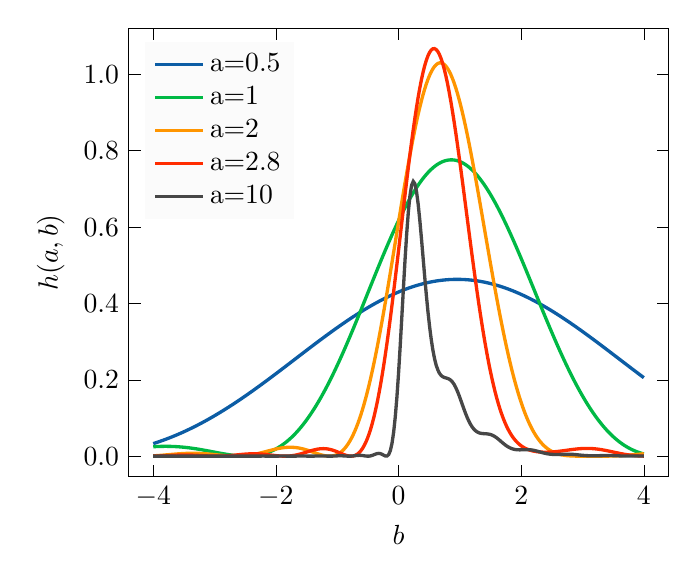
\begin{tikzpicture}

\definecolor{darkgray158}{RGB}{158,158,158}
\definecolor{darkgray176}{RGB}{176,176,176}
\definecolor{darkorange2551490}{RGB}{255,149,0}
\definecolor{darkslategray71}{RGB}{71,71,71}
\definecolor{limegreen018569}{RGB}{0,185,69}
\definecolor{orangered255440}{RGB}{255,44,0}
\definecolor{slategray13291151}{RGB}{132,91,151}
\definecolor{teal1293165}{RGB}{12,93,165}

\begin{axis}[
legend cell align={left},
legend style={
	fill=black!2,
  fill opacity=0.8,
  draw opacity=1,
  text opacity=1,
  at={(0.03,0.97)},
  anchor=north west,
  draw=none
},
tick pos=both,
x grid style={darkgray176},
xlabel={\(\displaystyle b\)},
xmin=-4.4, xmax=4.4,
xtick style={color=black},
xtick={-6,-4,-2,0,2,4,6},
xticklabels={
  \(\displaystyle {\ensuremath{-}6}\),
  \(\displaystyle {\ensuremath{-}4}\),
  \(\displaystyle {\ensuremath{-}2}\),
  \(\displaystyle {0}\),
  \(\displaystyle {2}\),
  \(\displaystyle {4}\),
  \(\displaystyle {6}\)
},
y grid style={darkgray176},
ylabel={\(\displaystyle h(a,b)\)},
ymin=-0.0533755941486969, ymax=1.12088747765006,
ytick style={color=black},
ytick={-0.2,0,0.2,0.4,0.6,0.8,1,1.2},
yticklabels={
  \(\displaystyle {\ensuremath{-}0.2}\),
  \(\displaystyle {0.0}\),
  \(\displaystyle {0.2}\),
  \(\displaystyle {0.4}\),
  \(\displaystyle {0.6}\),
  \(\displaystyle {0.8}\),
  \(\displaystyle {1.0}\),
  \(\displaystyle {1.2}\)
}
]
\addplot [very thick, teal1293165]
table {%
-4 0.0329347308512046
-3.97333333333333 0.0343055825245623
-3.94666666666667 0.0357080043590585
-3.92 0.0371420839779771
-3.89333333333333 0.038607898881193
-3.86666666666667 0.0401055163340945
-3.84 0.0416349932601001
-3.81333333333333 0.0431963761368276
-3.78666666666667 0.044789700895989
-3.76 0.0464149928270652
-3.73333333333333 0.0480722664848272
-3.70666666666667 0.0497615256007613
-3.68 0.051482762998457
-3.65333333333333 0.0532359605130127
-3.62666666666667 0.0550210889145177
-3.6 0.0568381078356582
-3.57333333333333 0.0586869657035041
-3.54666666666667 0.0605675996755226
-3.52 0.0624799355798691
-3.49333333333333 0.0644238878599992
-3.46666666666667 0.0663993595236489
-3.44 0.0684062420962228
-3.41333333333333 0.070444415578633
-3.38666666666667 0.0725137484096269
-3.36 0.07461409743264
-3.33333333333333 0.0767453078672096
-3.30666666666667 0.078907213284981
-3.28 0.0810996355903408
-3.25333333333333 0.0833223850056993
-3.22666666666667 0.0855752600614574
-3.2 0.0878580475906748
-3.17333333333333 0.0901705227284692
-3.14666666666667 0.092512448916163
-3.12 0.0948835779101949
-3.09333333333333 0.0972836497958193
-3.06666666666667 0.0997123930056014
-3.04 0.102169524342722
-3.01333333333333 0.104654749009104
-2.98666666666667 0.107167760638366
-2.96 0.109708241333611
-2.93333333333333 0.112275861710054
-2.90666666666667 0.114870280942481
-2.88 0.117491146817557
-2.85333333333333 0.120138095790962
-2.82666666666667 0.122810753049354
-2.8 0.125508732577165
-2.77333333333333 0.128231637228196
-2.74666666666667 0.130979058802024
-2.72 0.133750578125188
-2.69333333333333 0.136545765137146
-2.66666666666667 0.13936417898099
-2.64 0.142205368098883
-2.61333333333333 0.145068870332208
-2.58666666666667 0.147954213026396
-2.56 0.150860913140419
-2.53333333333333 0.153788477360896
-2.50666666666667 0.156736402220797
-2.48 0.159704174222713
-2.45333333333333 0.162691269966641
-2.42666666666667 0.165697156282259
-2.4 0.168721290365642
-2.37333333333333 0.171763119920391
-2.34666666666667 0.174822083303106
-2.32 0.177897609673175
-2.29333333333333 0.180989119146835
-2.26666666666667 0.184096022955429
-2.24 0.187217723607834
-2.21333333333333 0.190353615056983
-2.18666666666667 0.193503082870441
-2.16 0.196665504404969
-2.13333333333333 0.199840248985009
-2.10666666666667 0.203026678085035
-2.08 0.206224145515713
-2.05333333333333 0.209431997613777
-2.02666666666667 0.212649573435588
-2 0.215876204954269
-1.97333333333333 0.219111217260383
-1.94666666666667 0.222353928766039
-1.92 0.225603651412385
-1.89333333333333 0.228859690880394
-1.86666666666667 0.232121346804863
-1.84 0.235387912991552
-1.81333333333333 0.238658677637377
-1.78666666666667 0.241932923553573
-1.76 0.245209928391743
-1.73333333333333 0.248488964872702
-1.70666666666667 0.251769301018048
-1.68 0.255050200384321
-1.65333333333333 0.258330922299734
-1.62666666666667 0.261610722103301
-1.6 0.264888851386343
-1.57333333333333 0.268164558236221
-1.54666666666667 0.271437087482236
-1.52 0.27470568094357
-1.49333333333333 0.277969577679209
-1.46666666666667 0.28122801423969
-1.44 0.284480224920648
-1.41333333333333 0.287725442017976
-1.38666666666667 0.290962896084573
-1.36 0.294191816188525
-1.33333333333333 0.297411430172636
-1.30666666666667 0.300620964915204
-1.28 0.303819646591929
-1.25333333333333 0.307006700938847
-1.22666666666667 0.310181353516198
-1.2 0.3133428299731
-1.17333333333333 0.316490356312922
-1.14666666666667 0.31962315915927
-1.12 0.322740466022457
-1.09333333333333 0.325841505566335
-1.06666666666667 0.328925507875417
-1.04 0.331991704722147
-1.01333333333333 0.335039329834218
-0.986666666666666 0.33806761916182
-0.96 0.34107581114473
-0.933333333333333 0.344063146979095
-0.906666666666666 0.347028870883838
-0.88 0.349972230366538
-0.853333333333333 0.352892476488702
-0.826666666666667 0.355788864130307
-0.8 0.35866065225349
-0.773333333333333 0.361507104165296
-0.746666666666667 0.36432748777936
-0.72 0.367121075876414
-0.693333333333333 0.369887146363516
-0.666666666666667 0.372624982531882
-0.64 0.375333873313218
-0.613333333333333 0.378013113534447
-0.586666666666666 0.380662004170715
-0.56 0.383279852596561
-0.533333333333333 0.385865972835188
-0.506666666666666 0.388419685805655
-0.48 0.390940319567959
-0.453333333333333 0.393427209565853
-0.426666666666666 0.395879698867326
-0.4 0.398297138402612
-0.373333333333333 0.40067888719966
-0.346666666666666 0.403024312616948
-0.32 0.40533279057354
-0.293333333333333 0.407603705776275
-0.266666666666667 0.409836451944029
-0.24 0.412030432028923
-0.213333333333333 0.414185058434368
-0.186666666666667 0.416299753229916
-0.16 0.418373948362742
-0.133333333333333 0.420407085865729
-0.106666666666666 0.422398618062046
-0.0799999999999996 0.424348007766118
-0.0533333333333332 0.426254728480924
-0.0266666666666664 0.428118264591521
0 0.429938111554715
0.0266666666666673 0.431713776084811
0.0533333333333337 0.433444776335326
0.0800000000000001 0.435130642076641
0.106666666666667 0.436770914869454
0.133333333333334 0.438365148234011
0.16 0.439912907815012
0.186666666666667 0.441413771542119
0.213333333333334 0.442867329786034
0.24 0.444273185510015
0.266666666666667 0.445630954416829
0.293333333333334 0.44694026509104
0.32 0.448200759136583
0.346666666666667 0.449412091309552
0.373333333333334 0.45057392964618
0.4 0.451685955585891
0.426666666666667 0.452747864089447
0.453333333333334 0.453759363752083
0.48 0.454720176911597
0.506666666666667 0.455630039751357
0.533333333333333 0.456488702398175
0.56 0.457295929014998
0.586666666666667 0.458051497888383
0.613333333333333 0.458755201510722
0.640000000000001 0.459406846657171
0.666666666666667 0.460006254457259
0.693333333333333 0.460553260461141
0.720000000000001 0.461047714700458
0.746666666666667 0.461489481743806
0.773333333333333 0.461878440746755
0.800000000000001 0.462214485496409
0.826666666666667 0.462497524450524
0.853333333333333 0.462727480771076
0.88 0.462904292352385
0.906666666666667 0.463027911843676
0.933333333333334 0.463098306666133
0.96 0.463115459024415
0.986666666666667 0.463079365912625
1.01333333333333 0.462990039114751
1.04 0.462847505199542
1.06666666666667 0.462651805509874
1.09333333333333 0.462402996146553
1.12 0.462101147946608
1.14666666666667 0.461746346456066
1.17333333333333 0.461338691897206
1.2 0.460878299130343
1.22666666666667 0.460365297610119
1.25333333333333 0.459799831336357
1.28 0.459182058799466
1.30666666666667 0.458512152920448
1.33333333333333 0.457790300985517
1.36 0.45701670457537
1.38666666666667 0.456191579489124
1.41333333333333 0.455315155662983
1.44 0.454387677083634
1.46666666666667 0.453409401696432
1.49333333333333 0.452380601308417
1.52 0.451301561486199
1.54666666666667 0.450172581448739
1.57333333333333 0.448993973955109
1.6 0.447766065187253
1.62666666666667 0.446489194627803
1.65333333333333 0.445163714933018
1.68 0.443789991800883
1.70666666666667 0.442368403834438
1.73333333333333 0.440899342400401
1.76 0.439383211483118
1.78666666666667 0.437820427533954
1.81333333333333 0.436211419316128
1.84 0.434556627745125
1.86666666666667 0.432856505724699
1.89333333333333 0.431111517978574
1.92 0.429322140877901
1.94666666666667 0.427488862264542
1.97333333333333 0.425612181270279
2 0.423692608131998
2.02666666666667 0.42173066400295
2.05333333333333 0.419726880760165
2.08 0.417681800808093
2.10666666666667 0.415595976878565
2.13333333333333 0.413469971827176
2.16 0.411304358426138
2.18666666666667 0.409099719153736
2.21333333333333 0.406856645980441
2.24 0.404575740151819
2.26666666666667 0.402257611968251
2.29333333333333 0.399902880561669
2.32 0.397512173669291
2.34666666666667 0.395086127404532
2.37333333333333 0.392625386025156
2.4 0.390130601698768
2.42666666666667 0.387602434265763
2.45333333333333 0.385041550999811
2.48 0.382448626366009
2.50666666666667 0.379824341776758
2.53333333333333 0.377169385345538
2.56 0.37448445163861
2.58666666666667 0.371770241424805
2.61333333333333 0.369027461423479
2.64 0.36625682405077
2.66666666666667 0.363459047164211
2.69333333333333 0.360634853805871
2.72 0.357784971944089
2.74666666666667 0.354910134213924
2.77333333333333 0.352011077656439
2.8 0.3490885434569
2.82666666666667 0.346143276682054
2.85333333333333 0.34317602601653
2.88 0.340187543498519
2.90666666666667 0.337178584254845
2.93333333333333 0.334149906235493
2.96 0.331102269947775
2.98666666666667 0.328036438190168
3.01333333333333 0.324953175786001
3.04 0.32185324931706
3.06666666666667 0.318737426857232
3.09333333333333 0.31560647770632
3.12 0.312461172124094
3.14666666666667 0.309302281064733
3.17333333333333 0.306130575911743
3.2 0.302946828213464
3.22666666666667 0.299751809419277
3.25333333333333 0.296546290616614
3.28 0.29333104226889
3.30666666666667 0.290106833954447
3.33333333333333 0.286874434106628
3.36 0.283634609755082
3.38666666666667 0.280388126268413
3.41333333333333 0.277135747098256
3.44 0.273878233524907
3.46666666666667 0.27061634440459
3.49333333333333 0.267350835918487
3.52 0.26408246132358
3.54666666666667 0.260811970705484
3.57333333333333 0.257540110733284
3.6 0.254267624416528
3.62666666666667 0.250995250864464
3.65333333333333 0.247723725047591
3.68 0.244453777561638
3.70666666666667 0.241186134394062
3.73333333333333 0.237921516693156
3.76 0.23466064053983
3.78666666666667 0.231404216722204
3.81333333333333 0.228152950513041
3.84 0.224907541450157
3.86666666666667 0.221668683119853
3.89333333333333 0.218437062943467
3.92 0.21521336196713
3.94666666666667 0.211998254654792
3.97333333333333 0.208792408684606
4 0.205596484748741
};
\addlegendentry{a=0.5}
\addplot [very thick, limegreen018569]
table {%
-4 0.024690981021491
-3.97333333333333 0.0249436970430803
-3.94666666666667 0.0251636699097087
-3.92 0.02534987337496
-3.89333333333333 0.0255013564331003
-3.86666666666667 0.025617247844242
-3.84 0.0256967605814365
-3.81333333333333 0.0257391961886967
-3.78666666666667 0.0257439490389892
-3.76 0.0257105104812876
-3.73333333333333 0.0256384728658558
-3.70666666666667 0.0255275334370373
-3.68 0.0253774980829528
-3.65333333333333 0.0251882849316571
-3.62666666666667 0.0249599277834883
-3.6 0.0246925793695361
-3.57333333333333 0.0243865144263842
-3.54666666666667 0.0240421325775262
-3.52 0.0236599610121275
-3.49333333333333 0.0232406569520967
-3.46666666666667 0.0227850098987473
-3.44 0.02229394365067
-3.41333333333333 0.0217685180847913
-3.38666666666667 0.0212099306929818
-3.36 0.0206195178669713
-3.33333333333333 0.0199987559247532
-3.30666666666667 0.0193492618721003
-3.28 0.0186727938932721
-3.25333333333333 0.017971251565468
-3.22666666666667 0.0172466757920761
-3.2 0.0165012484502744
-3.17333333333333 0.0157372917490641
-3.14666666666667 0.0149572672943523
-3.12 0.0141637748582531
-3.09333333333333 0.0133595508503356
-3.06666666666667 0.0125474664891217
-3.04 0.0117305256727208
-3.01333333333333 0.0109118625480766
-2.98666666666667 0.0100947387789011
-2.96 0.00928254051297993
-2.93333333333333 0.00847877505013573
-2.90666666666667 0.00768706721275676
-2.88 0.00691115542141238
-2.85333333333333 0.00615488747869294
-2.82666666666667 0.00542221606503341
-2.8 0.00471719395089391
-2.77333333333333 0.00404396893028547
-2.74666666666667 0.00340677848124085
-2.72 0.0028099441594346
-2.69333333333333 0.00225786573175509
-2.66666666666667 0.00175501505722521
-2.64 0.00130592972324815
-2.61333333333333 0.000915206445728139
-2.58666666666667 0.00058749424217749
-2.56 0.000327487387468429
-2.53333333333333 0.000139918162422399
-2.50666666666667 2.95494059495579e-05
-2.48 1.16688195255275e-06
-2.45333333333333 5.95714726949216e-05
-2.42666666666667 0.000209571210800452
-2.4 0.000455973162496881
-2.37333333333333 0.000803575175143372
-2.34666666666667 0.00125715750248547
-2.32 0.00182147432146274
-2.29333333333333 0.00250124515475145
-2.26666666666667 0.00330114621355863
-2.24 0.00422580167549103
-2.21333333333333 0.00527977491260163
-2.18666666666667 0.0064675596849747
-2.16 0.00779357131543197
-2.13333333333333 0.00926213786114275
-2.10666666666667 0.0108774912980894
-2.08 0.0126437587344764
-2.05333333333333 0.0145649536692844
-2.02666666666667 0.0166449673122413
-2 0.0188875599815402
-1.97333333333333 0.0212963525956382
-1.94666666666667 0.0238748182754646
-1.92 0.0266262740733137
-1.89333333333333 0.0295538728446207
-1.86666666666667 0.0326605952787049
-1.84 0.0359492421044302
-1.81333333333333 0.039422426486544
-1.78666666666667 0.0430825666282625
-1.76 0.0469318785954294
-1.73333333333333 0.0509723693772921
-1.70666666666667 0.0552058301986662
-1.68 0.059633830097901
-1.65333333333333 0.0642577097847158
-1.62666666666667 0.0690785757915803
-1.6 0.074097294931892
-1.57333333333333 0.0793144890777643
-1.54666666666667 0.0847305302697472
-1.52 0.0903455361703254
-1.49333333333333 0.096159365872482
-1.46666666666667 0.102171616074094
-1.44 0.108381617628321
-1.41333333333333 0.114788432479563
-1.38666666666667 0.121390850993948
-1.36 0.128187389692642
-1.33333333333333 0.135176289395636
-1.30666666666667 0.142355513782978
-1.28 0.149722748379699
-1.25333333333333 0.15727539996999
-1.22666666666667 0.165010596445454
-1.2 0.172925187091495
-1.17333333333333 0.181015743315166
-1.14666666666667 0.189278559817037
-1.12 0.197709656208841
-1.09333333333333 0.206304779077902
-1.06666666666667 0.215059404498542
-1.04 0.223968740989879
-1.01333333333333 0.233027732918599
-0.986666666666666 0.24223106434455
-0.96 0.251573163306124
-0.933333333333333 0.261048206541661
-0.906666666666666 0.270650124642272
-0.88 0.280372607630701
-0.853333333333333 0.290209110960075
-0.826666666666667 0.300152861925555
-0.8 0.310196866481224
-0.773333333333333 0.32033391645371
-0.746666666666667 0.330556597143297
-0.72 0.340857295302631
-0.693333333333333 0.35122820748228
-0.666666666666667 0.361661348731828
-0.64 0.372148561644397
-0.613333333333333 0.3826815257319
-0.586666666666666 0.393251767117645
-0.56 0.403850668532303
-0.533333333333333 0.414469479598632
-0.506666666666666 0.425099327389811
-0.48 0.43573122724566
-0.453333333333333 0.446356093830487
-0.426666666666666 0.456964752415876
-0.4 0.467547950371149
-0.373333333333333 0.478096368843935
-0.346666666666666 0.488600634612746
-0.32 0.499051332093181
-0.293333333333333 0.509439015478997
-0.266666666666667 0.519754220998929
-0.24 0.529987479270035
-0.213333333333333 0.540129327727838
-0.186666666666667 0.55017032311361
-0.16 0.56010105399876
-0.133333333333333 0.569912153326263
-0.106666666666666 0.579594310948967
-0.0799999999999996 0.589138286144491
-0.0533333333333332 0.59853492008648
-0.0266666666666664 0.607775148251918
0 0.616850012744341
0.0266666666666673 0.625750674512783
0.0533333333333337 0.634468425446481
0.0800000000000001 0.642994700325503
0.106666666666667 0.651321088607612
0.133333333333334 0.659439346032047
0.16 0.667341406020957
0.186666666666667 0.675019390859784
0.213333333333334 0.682465622637959
0.24 0.689672633931896
0.266666666666667 0.696633178212492
0.293333333333334 0.703340239959874
0.32 0.709787044468584
0.346666666666667 0.715967067326866
0.373333333333334 0.721874043554305
0.4 0.727501976382576
0.426666666666667 0.732845145664701
0.453333333333334 0.737898115898746
0.48 0.742655743852649
0.506666666666667 0.747113185777454
0.533333333333333 0.751265904196914
0.56 0.755109674262193
0.586666666666667 0.758640589661089
0.613333333333333 0.761855068071984
0.640000000000001 0.764749856153427
0.666666666666667 0.767322034061175
0.693333333333333 0.769569019485177
0.720000000000001 0.771488571199918
0.746666666666667 0.773078792122265
0.773333333333333 0.774338131871932
0.800000000000001 0.775265388830379
0.826666666666667 0.775859711694902
0.853333333333333 0.776120600525568
0.88 0.776047907283396
0.906666666666667 0.775641835859179
0.933333333333334 0.774902941593143
0.96 0.773832130286492
0.986666666666667 0.772430656706809
1.01333333333333 0.770700122590141
1.04 0.768642474143405
1.06666666666667 0.76625999905159
1.09333333333333 0.76355532299521
1.12 0.760531405684099
1.14666666666667 0.75719153641458
1.17333333333333 0.753539329157853
1.2 0.749578717188086
1.22666666666667 0.74531394725975
1.25333333333333 0.740749573344148
1.28 0.735890449936099
1.30666666666667 0.730741724942314
1.33333333333333 0.725308832163749
1.36 0.719597483384854
1.38666666666667 0.713613660083268
1.41333333333333 0.707363604774247
1.44 0.700853812004509
1.46666666666667 0.694091019010919
1.49333333333333 0.687082196059886
1.52 0.67983453648385
1.54666666666667 0.672355446431731
1.57333333333333 0.664652534350708
1.6 0.656733600216918
1.62666666666667 0.648606624533339
1.65333333333333 0.640279757113137
1.68 0.631761305667382
1.70666666666667 0.623059724215995
1.73333333333333 0.614183601341343
1.76 0.605141648303837
1.78666666666667 0.59594268703921
1.81333333333333 0.586595638057247
1.84 0.577109508261806
1.86666666666667 0.567493378712063
1.89333333333333 0.55775639234487
1.92 0.547907741678268
1.94666666666667 0.537956656515867
1.97333333333333 0.527912391672023
2 0.517784214737397
2.02666666666667 0.507581393904411
2.05333333333333 0.497313185871959
2.08 0.486988823848398
2.10666666666667 0.476617505671695
2.13333333333333 0.466208382065246
2.16 0.455770545047549
2.18666666666667 0.445313016513615
2.21333333333333 0.434844737005559
2.24 0.42437455468939
2.26666666666667 0.41391121455461
2.29333333333333 0.403463347852744
2.32 0.393039461790334
2.34666666666667 0.382647929491583
2.37333333333333 0.372296980245072
2.4 0.361994690048529
2.42666666666667 0.351748972464983
2.45333333333333 0.341567569803006
2.48 0.331458044633123
2.50666666666667 0.321427771651771
2.53333333333333 0.311483929903551
2.56 0.301633495371795
2.58666666666667 0.291883233946752
2.61333333333333 0.282239694780007
2.64 0.272709204032951
2.66666666666667 0.263297859026461
2.69333333333333 0.254011522798083
2.72 0.244855819072357
2.74666666666667 0.235836127649096
2.77333333333333 0.22695758021363
2.8 0.218225056572349
2.82666666666667 0.209643181315999
2.85333333333333 0.201216320912457
2.88 0.192948581229949
2.90666666666667 0.184843805490872
2.93333333333333 0.176905572655625
2.96 0.169137196235102
2.98666666666667 0.161541723529755
3.01333333333333 0.15412193529234
3.04 0.14688034581081
3.06666666666667 0.139819203407011
3.09333333333333 0.1329404913462
3.12 0.126245929151648
3.14666666666667 0.119736974317976
3.17333333333333 0.113414824416146
3.2 0.107280419582445
3.22666666666667 0.101334445383129
3.25333333333333 0.0955773360458178
3.28 0.0900092780481442
3.30666666666667 0.0846302140535922
3.33333333333333 0.0794398471839359
3.36 0.0744376456171627
3.38666666666667 0.0696228474992971
3.41333333333333 0.0649944661580547
3.44 0.0605512956058536
3.46666666666667 0.0562919163192683
3.49333333333333 0.0522147012816604
3.52 0.0483178222753529
3.54666666666667 0.0445992564093958
3.57333333333333 0.0410567928686863
3.6 0.0376880398699321
3.62666666666667 0.0344904318097185
3.65333333333333 0.0314612365897415
3.68 0.0285975631040928
3.70666666666667 0.025896368873334
3.73333333333333 0.0233544678100046
3.76 0.0209685381001082
3.78666666666667 0.0187351301850835
3.81333333333333 0.0166506748287439
3.84 0.0147114912536796
3.86666666666667 0.0129137953316573
3.89333333333333 0.0112537078126229
3.92 0.00972726257701164
3.94666666666667 0.00833041489620017
3.97333333333333 0.00705904968608873
4 0.00590898973898823
};
\addlegendentry{a=1}
\addplot [very thick, darkorange2551490]
table {%
-4 0.00085925731227897
-3.97333333333333 0.0011006045740373
-3.94666666666667 0.00136828628602947
-3.92 0.00166028779598706
-3.89333333333333 0.0019742700639771
-3.86666666666667 0.00230758780627486
-3.84 0.00265731153105493
-3.81333333333333 0.00302025332503534
-3.78666666666667 0.00339299620630726
-3.76 0.00377192681557755
-3.73333333333333 0.00415327117641089
-3.70666666666667 0.00453313321525019
-3.68 0.00490753569447216
-3.65333333333333 0.00527246317694519
-3.62666666666667 0.00562390660891911
-3.6 0.00595790908000058
-3.57333333333333 0.00627061229481696
-3.54666666666667 0.00655830327110031
-3.52 0.00681746076362727
-3.49333333333333 0.00704480090300403
-3.46666666666667 0.00723732153290908
-3.44 0.00739234472927651
-3.41333333333333 0.00750755699014926
-3.38666666666667 0.00758104659563104
-3.36 0.00761133765353921
-3.33333333333333 0.00759742036798243
-3.30666666666667 0.00753877709506225
-3.28 0.00743540378209696
-3.25333333333333 0.00728782642397584
-3.22666666666667 0.00709711221223782
-3.2 0.00686487509891031
-3.17333333333333 0.00659327554769713
-3.14666666666667 0.00628501429935327
-3.12 0.00594332003558958
-3.09333333333333 0.00557193088610705
-3.06666666666667 0.00517506978584533
-3.04 0.00475741375367207
-3.01333333333333 0.0043240572289497
-2.98666666666667 0.00388046966806563
-2.96 0.00343244766847589
-2.93333333333333 0.00298606195242841
-2.90666666666667 0.00254759960565253
-2.88 0.00212350202726414
-2.85333333333333 0.00172029910529095
-2.82666666666667 0.00134454018693132
-2.8 0.00100272246330052
-2.77333333333333 0.000701217434397522
-2.74666666666667 0.000446196160775792
-2.72 0.000243554043399569
-2.69333333333333 9.88359019251278e-05
-2.66666666666667 1.7162143731863e-05
-2.64 3.15683105649061e-06
-2.61333333333333 6.08784612323935e-05
-2.58666666666667 0.000193754275043875
-2.56 0.000404518900375799
-2.53333333333333 0.000695158122548143
-2.50666666666667 0.00106685854891768
-2.48 0.00151996390352575
-2.45333333333333 0.00205393864786717
-2.42666666666667 0.00266733957642134
-2.4 0.00335779598067002
-2.37333333333333 0.0041219989132462
-2.34666666666667 0.00495570001501494
-2.32 0.00585372029273803
-2.29333333333333 0.0068099691540624
-2.26666666666667 0.00781747392049017
-2.24 0.00886841994839748
-2.21333333333333 0.00995420139378503
-2.18666666666667 0.0110654825590273
-2.16 0.0121922696602537
-2.13333333333333 0.0133239927529816
-2.10666666666667 0.0144495974521121
-2.08 0.0155576459812904
-2.05333333333333 0.0166364269868386
-2.02666666666667 0.0176740734539128
-2 0.01865868796814
-1.97333333333333 0.0195784744756661
-1.94666666666667 0.0204218756091868
-1.92 0.0211777145680131
-1.89333333333333 0.0218353404673733
-1.86666666666667 0.0223847760067656
-1.84 0.02281686625
-1.81333333333333 0.0231234272612856
-1.78666666666667 0.0232973933029561
-1.76 0.0233329612717218
-1.73333333333333 0.0232257310321892
-1.70666666666667 0.0229728402991603
-1.68 0.0225730927242439
-1.65333333333333 0.0220270778577706
-1.62666666666667 0.0213372816840492
-1.6 0.0205081864666152
-1.57333333333333 0.0195463586902692
-1.54666666666667 0.018460523948165
-1.52 0.0172616276947373
-1.49333333333333 0.0159628808684584
-1.46666666666667 0.0145797894818178
-1.44 0.0131301673789583
-1.41333333333333 0.0116341314734058
-1.38666666666667 0.0101140788985629
-1.36 0.00859464563125815
-1.33333333333333 0.00710264628275083
-1.30666666666667 0.00566699489120392
-1.28 0.00431860669372847
-1.25333333333333 0.003090281003565
-1.22666666666667 0.00201656546767252
-1.2 0.00113360213076418
-1.17333333333333 0.000478955882459827
-1.14666666666667 9.14260135008744e-05
-1.12 1.08417536600362e-05
-1.09333333333333 0.00027784280686145
-1.06666666666667 0.000933646036885854
-1.04 0.00201979958868944
-1.01333333333333 0.00357792585465567
-0.986666666666666 0.00564945481091941
-0.96 0.00827534935519307
-0.933333333333333 0.0114958243732935
-0.906666666666666 0.0153500613458923
-0.88 0.0198759203790526
-0.853333333333333 0.0251096516011193
-0.826666666666667 0.0310856079138288
-0.8 0.0378359611165756
-0.773333333333333 0.0453904234391177
-0.746666666666667 0.0537759765193426
-0.72 0.0630166098487896
-0.693333333333333 0.0731330706793544
-0.666666666666667 0.0841426273400054
-0.64 0.0960588478525776
-0.613333333333333 0.108891395660998
-0.586666666666666 0.122645844199117
-0.56 0.137323511919075
-0.533333333333333 0.15292131928552
-0.506666666666666 0.169431669111749
-0.48 0.186842351472746
-0.453333333333333 0.205136474278168
-0.426666666666666 0.224292420426579
-0.4 0.244283832291759
-0.373333333333333 0.265079624113992
-0.346666666666666 0.286644022685056
-0.32 0.308936636526611
-0.293333333333333 0.33191255356908
-0.266666666666667 0.355522467143562
-0.24 0.379712829903957
-0.213333333333333 0.404426035102077
-0.186666666666667 0.429600624446361
-0.16 0.455171521586365
-0.133333333333333 0.481070290082001
-0.106666666666666 0.507225414539829
-0.0799999999999996 0.533562603430062
-0.0533333333333332 0.560005111938474
-0.0266666666666664 0.586474083058536
0 0.612888904991846
0.0266666666666673 0.639167582800443
0.0533333333333337 0.665227122143965
0.0800000000000001 0.690983922838376
0.106666666666667 0.716354179892594
0.133333333333334 0.741254289614534
0.16 0.76560125833045
0.186666666666667 0.789313111230382
0.213333333333334 0.812309298839123
0.24 0.834511098616091
0.266666666666667 0.855842009208948
0.293333333333334 0.876228134924788
0.32 0.895598558038733
0.346666666666667 0.913885696632569
0.373333333333334 0.931025645745359
0.4 0.946958499722456
0.426666666666667 0.961628653769259
0.453333333333334 0.974985082849483
0.48 0.986981596214552
0.506666666666667 0.997577066009436
0.533333333333333 1.00673562856951
0.56 1.01442685720235
0.586666666666667 1.02062590543543
0.613333333333333 1.02531361990484
0.640000000000001 1.02847662225981
0.666666666666667 1.03010735966122
0.693333333333333 1.03020412365817
0.720000000000001 1.02877103743382
0.746666666666667 1.02581801161769
0.773333333333333 1.02136066906614
0.800000000000001 1.01542023921314
0.826666666666667 1.00802342278936
0.853333333333333 0.999202227896438
0.88 0.988993778604912
0.906666666666667 0.977440097416487
0.933333333333334 0.964587863093257
0.96 0.950488145507016
0.986666666666667 0.935196119299807
1.01333333333333 0.918770758271517
1.04 0.901274512520566
1.06666666666667 0.882772970459135
1.09333333333333 0.863334507904177
1.12 0.843029926509148
1.14666666666667 0.821932083848764
1.17333333333333 0.800115517499751
1.2 0.777656065474606
1.22666666666667 0.754630485362606
1.25333333333333 0.731116074513281
1.28 0.707190293561984
1.30666666666667 0.682930395546035
1.33333333333333 0.65841306279356
1.36 0.633714053685779
1.38666666666667 0.608907861298792
1.41333333333333 0.584067385822663
1.44 0.559263622535746
1.46666666666667 0.53456536698086
1.49333333333333 0.510038938849079
1.52 0.485747925926869
1.54666666666667 0.461752949305106
1.57333333333333 0.438111450884779
1.6 0.414877504045632
1.62666666666667 0.392101648171776
1.65333333333333 0.369830747553776
1.68 0.348107875011334
1.70666666666667 0.326972220405579
1.73333333333333 0.306459024036723
1.76 0.286599534752483
1.78666666666667 0.2674209924266
1.81333333333333 0.248946634306225
1.84 0.231195724572859
1.86666666666667 0.214183606315192
1.89333333333333 0.197921774974473
1.92 0.182417972194908
1.94666666666667 0.167676298893802
1.97333333333333 0.153697346259536
2 0.140478343290608
2.02666666666667 0.128013319406279
2.05333333333333 0.116293280589559
2.08 0.105306397466212
2.10666666666667 0.0950382036798787
2.13333333333333 0.0854718028929184
2.16 0.0765880827254785
2.18666666666667 0.068365933941336
2.21333333333333 0.0607824731980072
2.24 0.0538132677001897
2.26666666666667 0.0474325601293649
2.29333333333333 0.041613492267771
2.32 0.0363283257914408
2.34666666666667 0.0315486587738267
2.37333333333333 0.0272456365179996
2.4 0.0233901554206605
2.42666666666667 0.0199530586643843
2.45333333333333 0.0169053226346874
2.48 0.0142182330647096
2.50666666666667 0.0118635500215249
2.53333333333333 0.00981366096333904
2.56 0.0080417212150396
2.58666666666667 0.0065217813297086
2.61333333333333 0.0052289009247648
2.64 0.00413924870233078
2.66666666666667 0.00323018848323917
2.69333333333333 0.00248035120182791
2.72 0.00186969292339316
2.74666666666667 0.00137953905699282
2.77333333333333 0.000992615042382671
2.8 0.000693063890453092
2.82666666666667 0.000466451050902504
2.85333333333333 0.000299757168393087
2.88 0.000181359368517901
2.90666666666667 0.000101001787072713
2.93333333333333 4.97561199597271e-05
2.96 1.99730262230791e-05
2.98666666666667 5.22526297974743e-06
3.01333333333333 2.43468201344593e-07
3.04 8.4553534054406e-07
3.06666666666667 3.86054268335222e-06
3.09333333333333 7.04821012708131e-06
3.12 9.01485699501407e-06
3.14666666666667 9.1268267384051e-06
3.17333333333333 7.42232825280052e-06
3.2 4.52261942390524e-06
3.22666666666667 1.54342685666404e-06
3.25333333333333 7.45702522014191e-09
3.28 1.75880885827522e-06
3.30666666666667 8.88004663717823e-06
3.33333333333333 2.36126356649641e-05
3.36 4.82813821288128e-05
3.38666666666667 8.52234536170122e-05
3.41333333333333 0.000136722488574607
3.44 0.000204948232312182
3.46666666666667 0.000291902064746787
3.49333333333333 0.000399368711579604
3.52 0.000528874356818925
3.54666666666667 0.000681651301142661
3.57333333333333 0.000858609238244441
3.6 0.00106031315067606
3.62666666666667 0.00128696775841037
3.65333333333333 0.00153840838798752
3.68 0.00181409806821712
3.70666666666667 0.00211313060048708
3.73333333333333 0.00243423929822165
3.76 0.00277581104133222
3.78666666666667 0.00313590524795067
3.81333333333333 0.00351227732760926
3.84 0.00390240614754987
3.86666666666667 0.00430352501717448
3.89333333333333 0.00471265567488711
3.92 0.00512664474676351
3.94666666666667 0.00554220213760567
3.97333333333333 0.00595594081191482
4 0.006364417425018
};
\addlegendentry{a=2}
\addplot [very thick, orangered255440]
table {%
-4 0.000102875789801538
-3.97333333333333 0.000189466072940091
-3.94666666666667 0.000301221537347818
-3.92 0.000436621042347643
-3.89333333333333 0.000593576087663548
-3.86666666666667 0.000769462582427341
-3.84 0.000961165368958767
-3.81333333333333 0.0011651348603413
-3.78666666666667 0.00137745486933943
-3.76 0.00159392043738562
-3.73333333333333 0.00181012422230257
-3.70666666666667 0.00202154977796201
-3.68 0.00222366986368623
-3.65333333333333 0.00241204776084004
-3.62666666666667 0.00258243945308413
-3.6 0.00273089444879323
-3.57333333333333 0.00285385299198083
-3.54666666666667 0.00294823742362664
-3.52 0.00301153551951078
-3.49333333333333 0.00304187374345977
-3.46666666666667 0.00303807851521372
-3.44 0.0029997237978036
-3.41333333333333 0.00292716355725099
-3.38666666666667 0.00282154793345379
-3.36 0.00268482228028015
-3.33333333333333 0.0025197085793022
-3.30666666666667 0.00232966909867486
-3.28 0.00211885254920553
-3.25333333333333 0.00189202337598969
-3.22666666666667 0.00165447520809475
-3.2 0.00141192986247916
-3.17333333333333 0.00117042365343944
-3.14666666666667 0.00093618308735346
-3.12 0.000715492316631108
-3.09333333333333 0.000514554979388723
-3.06666666666667 0.000339353255887759
-3.04 0.000195507123490088
-3.01333333333333 8.81368840043462e-05
-2.98666666666667 2.17320671281653e-05
-2.96 2.9778712187068e-08
-2.93333333333333 2.59054615308599e-05
-2.90666666666667 0.000101278869217726
-2.88 0.000227037822446441
-2.85333333333333 0.000402982023122404
-2.82666666666667 0.000627788851454128
-2.8 0.000899002667765724
-2.77333333333333 0.00121304869249071
-2.74666666666667 0.00156527205178204
-2.72 0.001950002061419
-2.69333333333333 0.00236064128787865
-2.66666666666667 0.00278977838294087
-2.64 0.00322932314788594
-2.61333333333333 0.00367066175638103
-2.58666666666667 0.00410482956278031
-2.56 0.00452269845587668
-2.53333333333333 0.00491517529786552
-2.50666666666667 0.00527340762454551
-2.48 0.00558899248490047
-2.45333333333333 0.00585418407448381
-2.42666666666667 0.00606209567453514
-2.4 0.00620689135319707
-2.37333333333333 0.00628396292070765
-2.34666666666667 0.00629008775950665
-2.32 0.00622356337351241
-2.29333333333333 0.00608431481728459
-2.26666666666667 0.00587397157238531
-2.24 0.00559591093014415
-2.21333333333333 0.00525526551052801
-2.18666666666667 0.00485889318749742
-2.16 0.00441530839201812
-2.13333333333333 0.00393457451323211
-2.10666666666667 0.00342815790329263
-2.08 0.00290874479804274
-2.05333333333333 0.00239002327919998
-2.02666666666667 0.00188643320851258
-2 0.00141288784464633
-1.97333333333333 0.000984471593457989
-1.94666666666667 0.000616119026167749
-1.92 0.000322280912658215
-1.89333333333333 0.000116583544443539
-1.86666666666667 1.14880506435372e-05
-1.84 1.79567288478367e-05
-1.81333333333333 0.00014513361102034
-1.78666666666667 0.000400046554428869
-1.76 0.000787338082955221
-1.73333333333333 0.00130903200129067
-1.70666666666667 0.00196434246210966
-1.68 0.00274953168550471
-1.65333333333333 0.00365782191448068
-1.62666666666667 0.00467936644642856
-1.6 0.00580128371702899
-1.57333333333333 0.00700775744121066
-1.54666666666667 0.00828020474912764
-1.52 0.00959751310927602
-1.49333333333333 0.0109363456233799
-1.46666666666667 0.0122715130277042
-1.44 0.0135764094635205
-1.41333333333333 0.0148235078070654
-1.38666666666667 0.0159849090986729
-1.36 0.0170329394042913
-1.33333333333333 0.0179407863026579
-1.30666666666667 0.0186831661398741
-1.28 0.019237012250966
-1.25333333333333 0.0195821735349147
-1.22666666666667 0.0197021121036622
-1.2 0.0195845882227788
-1.17333333333333 0.0192223204355267
-1.14666666666667 0.0186136086240992
-1.12 0.0177629078200667
-1.09333333333333 0.0166813408356972
-1.06666666666667 0.0153871382507437
-1.04 0.0139059949541066
-1.01333333333333 0.0122713333016581
-0.986666666666666 0.0105244640022603
-0.96 0.00871463707210774
-0.933333333333333 0.00689897658823785
-0.906666666666666 0.00514229450763917
-0.88 0.00351678047830875
-0.853333333333333 0.00210156632981156
-0.826666666666667 0.000982165768157098
-0.8 0.000249791686107576
-0.773333333333333 5.55406945335143e-07
-0.746666666666667 0.000334554077890925
-0.72 0.00135485428891653
-0.693333333333333 0.0031663817837811
-0.666666666666667 0.00587472882333403
-0.64 0.00958489232807287
-0.613333333333333 0.0143999573406191
-0.586666666666666 0.0204197415841143
-0.56 0.0277394179268058
-0.533333333333333 0.036448132376283
-0.506666666666666 0.0466276358020627
-0.48 0.0583509479090262
-0.453333333333333 0.071681072046827
-0.426666666666666 0.0866697792358995
-0.4 0.103356479317318
-0.373333333333333 0.121767196393731
-0.346666666666666 0.141913664728372
-0.32 0.163792560019293
-0.293333333333333 0.187384879480913
-0.266666666666667 0.21265548246307
-0.24 0.239552801440854
-0.213333333333333 0.268008731141612
-0.186666666666667 0.29793870136668
-0.16 0.32924193674498
-0.133333333333333 0.361801904256116
-0.106666666666666 0.395486946915935
-0.0799999999999996 0.430151099562724
-0.0533333333333332 0.465635080252648
-0.0266666666666664 0.501767448404171
0 0.538365918557715
0.0266666666666673 0.575238816472303
0.0533333333333337 0.612186662297158
0.0800000000000001 0.649003863763232
0.106666666666667 0.685480500763774
0.133333333333334 0.721404181358757
0.16 0.75656194816575
0.186666666666667 0.790742213305306
0.213333333333334 0.823736699566194
0.24 0.855342365251375
0.266666666666667 0.885363290264936
0.293333333333334 0.91361250140101
0.32 0.939913715494423
0.346666666666667 0.964102980078505
0.373333333333334 0.986030192455237
0.4 1.00556047959851
0.426666666666667 1.02257542306106
0.453333333333334 1.03697411501454
0.48 1.04867403369253
0.506666666666667 1.05761172879621
0.533333333333333 1.06374330983086
0.56 1.06704473283185
0.586666666666667 1.06751188347739
0.613333333333333 1.06516045713497
0.640000000000001 1.0600256389138
0.666666666666667 1.05216158926017
0.693333333333333 1.04164074300324
0.720000000000001 1.02855293200224
0.746666666666667 1.01300434363062
0.773333333333333 0.995116329232823
0.800000000000001 0.975024078377488
0.826666666666667 0.952875176186448
0.853333333333333 0.928828062224634
0.88 0.903050410376117
0.906666666666667 0.875717449797131
0.933333333333334 0.847010247422395
0.96 0.817113972603489
0.986666666666667 0.786216164281793
1.01333333333333 0.75450502064884
1.04 0.722167730535662
1.06666666666667 0.689388864813652
1.09333333333333 0.656348844901208
1.12 0.623222504073522
1.14666666666667 0.590177755692007
1.17333333333333 0.557374380730583
1.2 0.524962945107425
1.22666666666667 0.493083855361872
1.25333333333333 0.461866559178245
1.28 0.431428895182186
1.30666666666667 0.401876594352114
1.33333333333333 0.373302933329165
1.36 0.345788537903166
1.38666666666667 0.319401333028059
1.41333333333333 0.294196633904108
1.44 0.270217370980423
1.46666666666667 0.247494440201092
1.49333333333333 0.226047168460786
1.52 0.205883883065943
1.54666666666667 0.187002573028469
1.57333333333333 0.169391629258825
1.6 0.153030650179827
1.62666666666667 0.137891298953382
1.65333333333333 0.12393819839813
1.68 0.111129849771475
1.70666666666667 0.0994195618868654
1.73333333333333 0.0887563775250173
1.76 0.079085984762472
1.78666666666667 0.0703516016659098
1.81333333333333 0.0624948237677911
1.84 0.0554564248278307
1.86666666666667 0.0491771025741204
1.89333333333333 0.0435981623847779
1.92 0.0386621331927721
1.94666666666667 0.0343133112497067
1.97333333333333 0.0304982287458158
2 0.0271660456306881
2.02666666666667 0.0242688642908201
2.05333333333333 0.0217619679957359
2.08 0.0196039852054825
2.10666666666667 0.0177569829220753
2.13333333333333 0.016186493251255
2.16 0.0148614782064049
2.18666666666667 0.0137542385237439
2.21333333333333 0.0128402728596027
2.24 0.0120980942019372
2.26666666666667 0.0115090106470797
2.29333333333333 0.0110568778694546
2.32 0.0107278306494806
2.34666666666667 0.0105100007283449
2.37333333333333 0.0103932280351943
2.4 0.0103687719919089
2.42666666666667 0.0104290291541754
2.45333333333333 0.0105672629076905
2.48 0.0107773503188837
2.50666666666667 0.011053550555367
2.53333333333333 0.0113902985578458
2.56 0.0117820268782589
2.58666666666667 0.0122230178142888
2.61333333333333 0.0127072871836688
2.64 0.0132285003079765
2.66666666666667 0.0137799200290871
2.69333333333333 0.0143543858754064
2.72 0.0149443228413864
2.74666666666667 0.0155417776532095
2.77333333333333 0.0161384798748829
2.8 0.0167259247695905
2.82666666666667 0.0172954744764956
2.85333333333333 0.0178384737969487
2.88 0.0183463767080381
2.90666666666667 0.0188108796356444
2.93333333333333 0.0192240575218609
2.96 0.0195784988093832
2.98666666666667 0.0198674356332957
3.01333333333333 0.0200848657521569
3.04 0.0202256630578266
3.06666666666667 0.0202856738683493
3.09333333333333 0.0202617966209069
3.12 0.0201520430321761
3.14666666666667 0.0199555792707798
3.17333333333333 0.0196727461800957
3.2 0.0193050580887143
3.22666666666667 0.0188551802397381
3.25333333333333 0.018326885348804
3.28 0.0177249902546549
3.30666666666667 0.0170552740466124
3.33333333333333 0.0163243794326223
3.36 0.015539699442981
3.38666666666667 0.0147092518428817
3.41333333333333 0.0138415438472707
3.44 0.0129454298912302
3.46666666666667 0.0120299653065341
3.49333333333333 0.0111042587898791
3.52 0.0101773265215057
3.54666666666667 0.00925795070674232
3.57333333333333 0.00835454517076409
3.6 0.00747503044301781
3.62666666666667 0.00662672052766267
3.65333333333333 0.00581622327622003
3.68 0.00504935596522566
3.70666666666667 0.00433107734240001
3.73333333333333 0.0036654370473592
3.76 0.00305554294505942
3.78666666666667 0.00250354653985963
3.81333333333333 0.00201064627303229
3.84 0.00157710815416402
3.86666666666667 0.00120230284414293
3.89333333333333 0.000884758000715714
3.92 0.000622224422617002
3.94666666666667 0.000411754289923129
3.97333333333333 0.000249789600592412
4 0.000132258749208685
};
\addlegendentry{a=2.8}
\addplot [very thick, darkslategray71]
table {%
-4 1.99136111090757e-05
-3.97333333333333 6.88352200423779e-06
-3.94666666666667 3.28440458246664e-07
-3.92 2.39046962012096e-06
-3.89333333333333 1.28457498685867e-05
-3.86666666666667 2.91025969904233e-05
-3.84 4.68657196877344e-05
-3.81333333333333 6.12981639687327e-05
-3.78666666666667 6.83681125032116e-05
-3.76 6.60069954422061e-05
-3.73333333333333 5.47479051413779e-05
-3.70666666666667 3.76500039081225e-05
-3.68 1.95097610715948e-05
-3.65333333333333 5.56033960334506e-06
-3.62666666666667 1.01510754686023e-08
-3.6 4.82702596892462e-06
-3.57333333333333 1.91173084110948e-05
-3.54666666666667 3.92922303288322e-05
-3.52 5.9998275160116e-05
-3.49333333333333 7.55727096376569e-05
-3.46666666666667 8.16305632130277e-05
-3.44 7.63403878959983e-05
-3.41333333333333 6.10200949406773e-05
-3.38666666666667 3.98640251780171e-05
-3.36 1.88509177133917e-05
-3.33333333333333 4.11443337295597e-06
-3.30666666666667 2.18003806370604e-07
-3.28 8.81677702822802e-06
-3.25333333333333 2.80960150024174e-05
-3.22666666666667 5.31694051713739e-05
-3.2 7.73565841478892e-05
-3.17333333333333 9.40090539768169e-05
-3.14666666666667 9.83883296685108e-05
-3.12 8.90688491715726e-05
-3.09333333333333 6.84541695402834e-05
-3.06666666666667 4.22306257300906e-05
-3.04 1.78757790459766e-05
-3.01333333333333 2.60921606041813e-06
-2.98666666666667 1.34384085668452e-06
-2.96 1.52153258553591e-05
-2.93333333333333 4.11250622457175e-05
-2.90666666666667 7.24620559971754e-05
-2.88 0.000100843059785161
-2.85333333333333 0.000118417472638412
-2.82666666666667 0.000120107692344237
-2.8 0.000105150395847909
-2.77333333333333 7.74774312243383e-05
-2.74666666666667 4.47845967406721e-05
-2.72 1.65006499322272e-05
-2.69333333333333 1.18713243852453e-06
-2.66666666666667 4.08076115789665e-06
-2.64 2.54779574186789e-05
-2.61333333333333 6.04514148690635e-05
-2.58666666666667 0.000100032601941247
-2.56 0.000133586042154717
-2.53333333333333 0.000151753791739077
-2.50666666666667 0.000149161937410452
-2.48 0.000126114279119404
-2.45333333333333 8.87514109396415e-05
-2.42666666666667 4.75642102757001e-05
-2.4 1.46104146007924e-05
-2.37333333333333 1.64272436698577e-07
-2.34666666666667 9.72151433483498e-06
-2.32 4.22227134093416e-05
-2.29333333333333 9.00530001950478e-05
-2.26666666666667 0.000140899898906856
-2.24 0.000181030016199106
-2.21333333333333 0.000199124015756049
-2.18666666666667 0.000189610942680092
-2.16 0.000154533803462429
-2.13333333333333 0.000103346513281471
-2.10666666666667 5.05975725068394e-05
-2.08 1.20509320304871e-05
-2.05333333333333 2.63909754321396e-07
-2.02666666666667 2.0847347705563e-05
-2 7.05033498174686e-05
-1.97333333333333 0.000137490364061044
-1.94666666666667 0.000204513178547311
-1.92 0.00025334935852966
-1.89333333333333 0.000269995074929327
-1.86666666666667 0.000248899407826856
-1.84 0.000195034380182259
-1.81333333333333 0.000123089667180621
-1.78666666666667 5.38539998619805e-05
-1.76 8.64527359763909e-06
-1.73333333333333 3.2546775239343e-06
-1.70666666666667 4.30955191066293e-05
-1.68 0.000121009044680269
-1.65333333333333 0.000218516684708653
-1.62666666666667 0.000310381427349807
-1.6 0.000371394855641686
-1.57333333333333 0.000383605726098175
-1.54666666666667 0.000341963565442601
-1.52 0.00025666448531881
-1.49333333333333 0.000151304652408501
-1.46666666666667 5.70733014828628e-05
-1.44 4.35614796063124e-06
-1.41333333333333 1.39523016105261e-05
-1.38666666666667 9.03778816974699e-05
-1.36 0.00021932138928935
-1.33333333333333 0.000370294742962585
-1.30666666666667 0.000504130983435758
-1.28 0.000583577866308384
-1.25333333333333 0.000584218468956596
-1.22666666666667 0.000502631080922546
-1.2 0.000359226201733069
-1.17333333333333 0.000194489902597713
-1.14666666666667 5.91220798093231e-05
-1.12 3.32577988938962e-07
-1.09333333333333 4.78529457701281e-05
-1.06666666666667 0.000203632654901482
-1.04 0.000438521636044866
-1.01333333333333 0.000697582794283473
-0.986666666666666 0.000913397525762471
-0.96 0.00102439894869746
-0.933333333333333 0.000993533939038621
-0.906666666666666 0.000821957027536573
-0.88 0.000553279404526275
-0.853333333333333 0.00026605744795037
-0.826666666666667 5.52557923856331e-05
-0.8 6.61851987393427e-06
-0.773333333333333 0.000170366969565249
-0.746666666666667 0.000541650467830218
-0.72 0.00105425564403427
-0.693333333333333 0.00159124516338889
-0.666666666666667 0.00201197480963607
-0.64 0.0021902877721987
-0.613333333333333 0.00205479628931546
-0.586666666666666 0.00162017236568316
-0.56 0.000999071241367595
-0.533333333333333 0.000387903352395072
-0.506666666666666 2.56425063503741e-05
-0.48 0.000132033686744228
-0.453333333333333 0.000838313064169277
-0.426666666666666 0.00212813560407123
-0.4 0.00380737892870577
-0.373333333333333 0.00551808606671526
-0.346666666666666 0.00680418391916179
-0.32 0.00722592197736039
-0.293333333333333 0.00650820629414698
-0.266666666666667 0.00469762003878944
-0.24 0.00229636089180289
-0.213333333333333 0.000340461129638066
-0.186666666666667 0.000395344315966373
-0.16 0.00445358159735119
-0.133333333333333 0.0147359102267494
-0.106666666666666 0.0334144010125443
-0.0799999999999996 0.0622928054074334
-0.0533333333333332 0.102490371132977
-0.0266666666666664 0.154179329588564
0 0.216421644143191
0.0266666666666673 0.287137842640963
0.0533333333333337 0.363221762473212
0.0800000000000001 0.440792955253275
0.106666666666667 0.515557119512215
0.133333333333334 0.583227978166318
0.16 0.639954446820786
0.186666666666667 0.682696375144788
0.213333333333334 0.709500585758731
0.24 0.719644774979368
0.266666666666667 0.713637191252604
0.293333333333334 0.693081275926459
0.32 0.660433025957158
0.346666666666667 0.618691762892563
0.373333333333334 0.571070485145347
0.4 0.52068970284075
0.426666666666667 0.470329687231056
0.453333333333334 0.422262610373396
0.48 0.378170925736915
0.506666666666667 0.33914439818047
0.533333333333333 0.305737763007099
0.56 0.278065482835694
0.586666666666667 0.255909769873907
0.613333333333333 0.238822185933639
0.640000000000001 0.226206171586795
0.666666666666667 0.21737585678849
0.693333333333333 0.211593602749463
0.720000000000001 0.208093510061766
0.746666666666667 0.206099900898326
0.773333333333333 0.204848623511412
0.800000000000001 0.203615686909508
0.826666666666667 0.201753387618791
0.853333333333333 0.198730017930164
0.88 0.194166517255486
0.906666666666667 0.187862675187735
0.933333333333334 0.179806797293992
0.96 0.170165665372219
0.986666666666667 0.159255359156737
1.01333333333333 0.147497111439526
1.04 0.135364997111696
1.06666666666667 0.123333357017243
1.09333333333333 0.111831281206689
1.12 0.101209480427355
1.14666666666667 0.0917220270938842
1.17333333333333 0.0835224630484845
1.2 0.0766713298836213
1.22666666666667 0.071150760337158
1.25333333333333 0.0668815629076875
1.28 0.06373911025647
1.30666666666667 0.0615659274918231
1.33333333333333 0.0601806582614562
1.36 0.0593845623143325
1.38666666666667 0.0589675012717197
1.41333333333333 0.0587153513013938
1.44 0.0584200315950375
1.46666666666667 0.057892140093442
1.49333333333333 0.0569749312026197
1.52 0.0555574359694293
1.54666666666667 0.053584186554816
1.57333333333333 0.0510593619186151
1.6 0.0480441266430043
1.62666666666667 0.0446472387046814
1.65333333333333 0.0410103200568565
1.68 0.0372901891210724
1.70666666666667 0.0336411117820866
1.73333333333333 0.030199650183657
1.76 0.0270740519170782
1.78666666666667 0.0243390356899341
1.81333333333333 0.0220356759422866
1.84 0.0201751474828449
1.86666666666667 0.0187445670702926
1.89333333333333 0.0177131452190738
1.92 0.0170372868950093
1.94666666666667 0.0166639908859287
1.97333333333333 0.0165326700361465
2 0.0165761261926912
2.02666666666667 0.0167217040441862
2.05333333333333 0.0168935570829773
2.08 0.0170165374294976
2.10666666666667 0.0170216105472332
2.13333333333333 0.016852084479776
2.16 0.0164695130235328
2.18666666666667 0.0158580089141865
2.21333333333333 0.0150259240852971
2.24 0.0140043615567471
2.26666666666667 0.0128426434074123
2.29333333333333 0.0116014997110004
2.32 0.0103452017558543
2.34666666666667 0.00913402889885266
2.37333333333333 0.00801830082994252
2.4 0.00703477893823567
2.42666666666667 0.00620566178004677
2.45333333333333 0.00553982271275572
2.48 0.00503550598059813
2.50666666666667 0.00468350822434286
2.53333333333333 0.00446995353785342
2.56 0.00437807679818863
2.58666666666667 0.00438885992574171
2.61333333333333 0.00448079013970467
2.64 0.00462930870995156
2.66666666666667 0.00480661502342554
2.69333333333333 0.00498236646120693
2.72 0.00512551479337516
2.74666666666667 0.00520713737781089
2.77333333333333 0.00520376951884756
2.8 0.00510052446864066
2.82666666666667 0.0048932622154613
2.85333333333333 0.00458924484725489
2.88 0.00420604686750565
2.90666666666667 0.00376888444615892
2.93333333333333 0.00330688357933776
2.96 0.00284903178432936
2.98666666666667 0.00242059666495381
3.01333333333333 0.00204064339531553
3.04 0.00172098780640312
3.06666666666667 0.00146656424740381
3.09333333333333 0.0012768625439924
3.12 0.00114787814072791
3.14666666666667 0.00107397163492716
3.17333333333333 0.00104915054987312
3.2 0.00106752526900979
3.22666666666667 0.00112297942455538
3.25333333333333 0.0012083496153561
3.28 0.00131456008408777
3.30666666666667 0.0014301665522885
3.33333333333333 0.00154163245036589
3.36 0.00163443180725797
3.38666666666667 0.0016948137723051
3.41333333333333 0.00171184856515911
3.44 0.00167926409475754
3.46666666666667 0.00159660688071362
3.49333333333333 0.00146941284725264
3.52 0.00130831086341103
3.54666666666667 0.00112723996238445
3.57333333333333 0.000941171047169727
3.6 0.000763831094098141
3.62666666666667 0.000605906718921504
3.65333333333333 0.00047406373934243
3.68 0.000370900783318636
3.70666666666667 0.000295718350714897
3.73333333333333 0.000245793063121494
3.76 0.000217748818442628
3.78666666666667 0.000208633879068638
3.81333333333333 0.000216435269776433
3.84 0.000239950842059591
3.86666666666667 0.000278139847529436
3.89333333333333 0.000329228582961389
3.92 0.000389916631071455
3.94666666666667 0.000454994778887694
3.97333333333333 0.000517560373330807
4 0.000569837100924757
};
\addlegendentry{a=10}
\end{axis}

\end{tikzpicture}

\end{frame}

\section{Mise en \oe uvre}

\begin{frame}{Choix du cristal doubleur}
Cristal de niobate de lithium polarisé périodiquement dopé au magnésium (MgO\hc PPLN) :
\begin{itemize}
\item $\chi^{(2)}$ important selon l'axe extraordinaire
\item[$\rightarrow$] bonne efficacité de conversion
\item effets non-linéaires parasites à haute intensité :
\begin{itemize}
\item inhomogénéités d'indice optique et couplage entre les faisceaux (effet photoréfractif)
\item absorption de l'infrarouge induite par le vert (\textit{green-induced infrared absorption---GRIIRA})
\end{itemize}
\end{itemize}
$\boldsymbol\rightarrow$ avantageux pour produire jusqu'à 2--3 watts de lumière verte
\end{frame}

\begin{frame}{Choix du cristal doubleur}
Cristal Covesion de longueur $L=\SI{20}{mm}$ \\
%5 bandes de périodes d'inversion
$\Lambda = \qtylist[list-units = single]{6.83; 6.86 ; 6.90 ; 6.93 ; 6,96}{\micro\meter}$
\begin{figure}
\centering
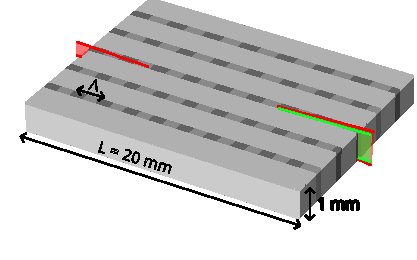
\includegraphics[height=5cm]{img/cristal2.pdf} %TODO fond
\end{figure}
\end{frame}

\begin{frame}{Montage}
\centering
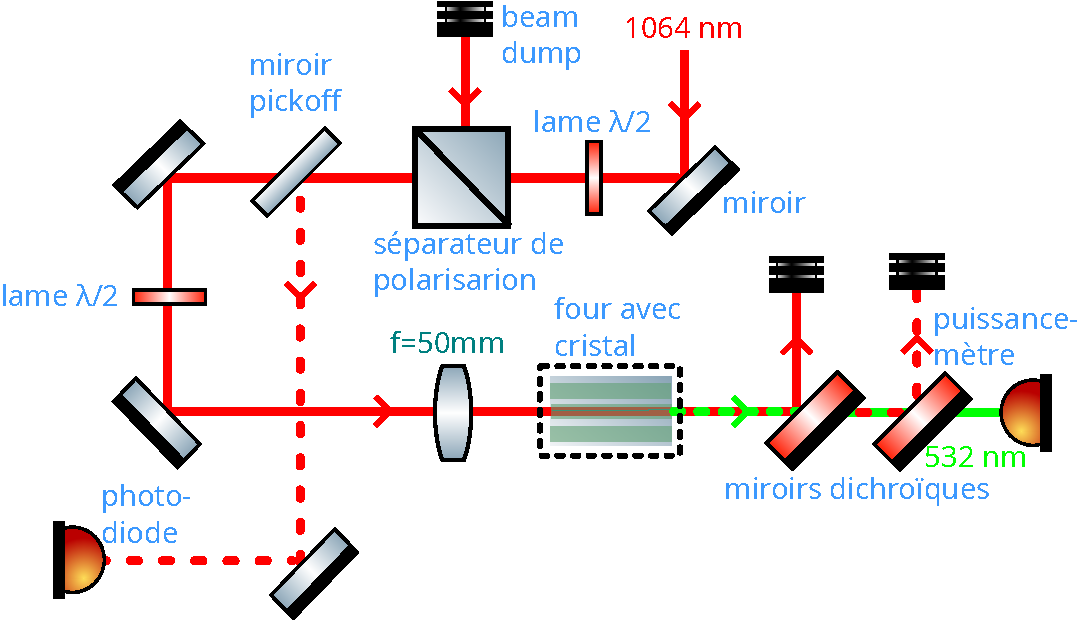
\includegraphics[height=6.4cm]{img/schema.pdf}
%\begin{overpic}[percent,height=6cm,grid,tics=5]{img/schema.pdf}
%\put(57,53){\small \color{red} \lmbd{1064}}
%\end{overpic}
\end{frame}

\begin{frame}{Estimation de la température optimale}
\centering
% This file was created with tikzplotlib v0.10.1.
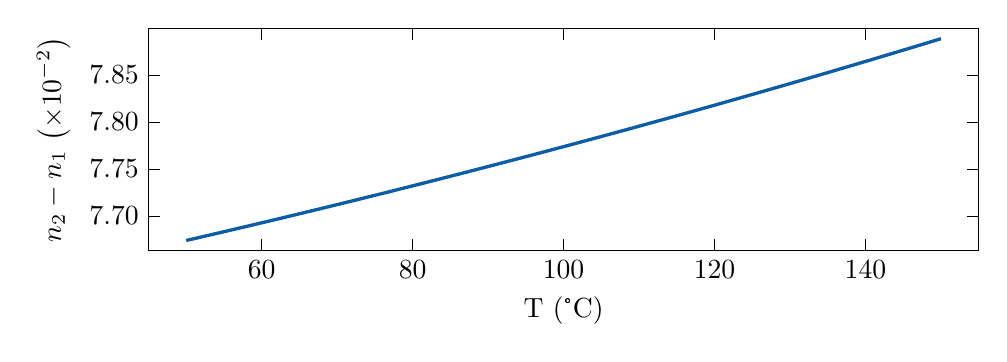
\begin{tikzpicture}

\definecolor{darkgray176}{RGB}{176,176,176}
\definecolor{teal1293165}{RGB}{12,93,165}

\begin{axis}[
width=\linewidth,
height=4.4cm,
tick pos=both,
x grid style={darkgray176},
xlabel={T (°C)},
xmin=45, xmax=155,
xtick style={color=black},
xtick={40,60,80,100,120,140,160},
xticklabels={
  \(\displaystyle {40}\),
  \(\displaystyle {60}\),
  \(\displaystyle {80}\),
  \(\displaystyle {100}\),
  \(\displaystyle {120}\),
  \(\displaystyle {140}\),
  \(\displaystyle {160}\)
},
y grid style={darkgray176},
ylabel={\(\displaystyle n_2-n_1\) \(\displaystyle \left(\times 10^{-2}\right)\)},
ymin=7.6629850784832, ymax=7.89936722344637,
ytick style={color=black},
ytick={7.65,7.7,7.75,7.8,7.85,7.9},
yticklabels={
  \(\displaystyle {7.65}\),
  \(\displaystyle {7.70}\),
  \(\displaystyle {7.75}\),
  \(\displaystyle {7.80}\),
  \(\displaystyle {7.85}\),
  \(\displaystyle {7.90}\)
}
]
\addplot [very thick, teal1293165]
table {%
50 7.67372972143607
50.2004008016032 7.67410055301299
50.4008016032064 7.6744716219225
50.6012024048096 7.67484292818015
50.8016032064128 7.67521447180144
51.002004008016 7.67558625280187
51.2024048096192 7.67595827119703
51.4028056112224 7.67633052700245
51.6032064128256 7.67670302023364
51.8036072144289 7.67707575090624
52.0040080160321 7.67744871903582
52.2044088176353 7.67782192463806
52.4048096192385 7.67819536772842
52.6052104208417 7.67856904832276
52.8056112224449 7.67894296643661
53.0060120240481 7.67931712208565
53.2064128256513 7.67969151528551
53.4068136272545 7.6800661460521
53.6072144288577 7.68044101440086
53.8076152304609 7.68081612034774
54.0080160320641 7.68119146390829
54.2084168336673 7.68156704509853
54.4088176352705 7.68194286393391
54.6092184368737 7.68231892043048
54.809619238477 7.68269521460399
55.0100200400802 7.68307174647016
55.2104208416834 7.68344851604494
55.4108216432866 7.68382552334415
55.6112224448898 7.68420276838357
55.811623246493 7.68458025117922
56.0120240480962 7.68495797174684
56.2124248496994 7.68533593010248
56.4128256513026 7.68571412626198
56.6132264529058 7.68609256024129
56.813627254509 7.68647123205644
57.0140280561122 7.68685014172328
57.2144288577154 7.68722928925785
57.4148296593186 7.68760867467617
57.6152304609218 7.68798829799429
57.8156312625251 7.68836815922813
58.0160320641283 7.68874825839378
58.2164328657315 7.68912859550737
58.4168336673347 7.68950917058491
58.6172344689379 7.68988998364253
58.8176352705411 7.69027103469626
59.0180360721443 7.69065232376223
59.2184368737475 7.69103385085668
59.4188376753507 7.69141561599564
59.6192384769539 7.69179761919534
59.8196392785571 7.69217986047197
60.0200400801603 7.6925623398417
60.2204408817635 7.6929450573207
60.4208416833667 7.69332801292535
60.6212424849699 7.69371120667177
60.8216432865731 7.69409463857613
61.0220440881764 7.69447830865491
61.2224448897796 7.69486221692426
61.4228456913828 7.69524636340053
61.623246492986 7.69563074810002
61.8236472945892 7.69601537103908
62.0240480961924 7.69640023223404
62.2244488977956 7.69678533170128
62.4248496993988 7.69717066945721
62.625250501002 7.69755624551811
62.8256513026052 7.69794205990051
63.0260521042084 7.69832811262079
63.2264529058116 7.69871440369543
63.4268537074148 7.69910093314077
63.627254509018 7.69948770097342
63.8276553106212 7.69987470720976
64.0280561122244 7.70026195186642
64.2284569138277 7.70064943495981
64.4288577154309 7.7010371565065
64.6292585170341 7.70142511652296
64.8296593186373 7.70181331502586
65.0300601202405 7.7022017520318
65.2304609218437 7.70259042755725
65.4308617234469 7.70297934161892
65.6312625250501 7.70336849423341
65.8316633266533 7.70375788541733
66.0320641282565 7.70414751518742
66.2324649298597 7.70453738356025
66.4328657314629 7.70492749055252
66.6332665330661 7.705317836181
66.8336673346693 7.70570842046241
67.0340681362725 7.70609924341339
67.2344689378758 7.70649030505077
67.434869739479 7.7068816053913
67.6352705410822 7.70727314445177
67.8356713426854 7.70766492224886
68.0360721442886 7.70805693879959
68.2364729458918 7.7084491941207
68.436873747495 7.70884168822894
68.6372745490982 7.70923442114126
68.8376753507014 7.70962739287455
69.0380761523046 7.71002060344563
69.2384769539078 7.71041405287143
69.438877755511 7.7108077411689
69.6392785571142 7.71120166835497
69.8396793587174 7.71159583444665
70.0400801603206 7.71199023946076
70.2404809619239 7.71238488341437
70.4408817635271 7.71277976632447
70.6412825651303 7.71317488820813
70.8416833667335 7.7135702490823
71.0420841683367 7.71396584896404
71.2424849699399 7.71436168787045
71.4428857715431 7.71475776581863
71.6432865731463 7.71515408282561
71.8436873747495 7.71555063890847
72.0440881763527 7.71594743408444
72.2444889779559 7.71634446837064
72.4448897795591 7.71674174178414
72.6452905811623 7.71713925434225
72.8456913827655 7.71753700606199
73.0460921843687 7.71793499696072
73.2464929859719 7.71833322705557
73.4468937875751 7.71873169636383
73.6472945891784 7.71913040490269
73.8476953907816 7.71952935268949
74.0480961923848 7.71992853974148
74.248496993988 7.72032796607598
74.4488977955912 7.72072763171026
74.6492985971944 7.72112753666163
74.8496993987976 7.72152768094752
75.0501002004008 7.72192806458527
75.250501002004 7.72232868759222
75.4509018036072 7.72272954998585
75.6513026052104 7.72313065178345
75.8517034068136 7.7235319930026
76.0521042084168 7.72393357366061
76.25250501002 7.72433539377495
76.4529058116233 7.7247374533632
76.6533066132264 7.7251397524428
76.8537074148297 7.72554229103117
77.0541082164329 7.72594506914595
77.2545090180361 7.72634808680457
77.4549098196393 7.72675134402476
77.6553106212425 7.72715484082389
77.8557114228457 7.72755857721967
78.0561122244489 7.72796255322974
78.2565130260521 7.72836676887159
78.4569138276553 7.72877122416298
78.6573146292585 7.7291759191215
78.8577154308617 7.72958085376474
79.0581162324649 7.72998602811055
79.2585170340681 7.73039144217651
79.4589178356713 7.73079709598039
79.6593186372746 7.73120298953991
79.8597194388778 7.73160912287287
80.060120240481 7.73201549599691
80.2605210420842 7.73242210892993
80.4609218436874 7.73282896168968
80.6613226452906 7.73323605429397
80.8617234468938 7.73364338676061
81.062124248497 7.7340509591076
81.2625250501002 7.73445877135255
81.4629258517034 7.73486682351359
81.6633266533066 7.73527511560843
81.8637274549098 7.73568364765498
82.064128256513 7.7360924196713
82.2645290581162 7.7365014316753
82.4649298597194 7.73691068368492
82.6653306613227 7.73732017571809
82.8657314629259 7.73772990779285
83.0661322645291 7.73813987992722
83.2665330661323 7.7385500921392
83.4669338677355 7.73896054444685
83.6673346693387 7.73937123686821
83.8677354709419 7.73978216942139
84.0681362725451 7.74019334212439
84.2685370741483 7.74060475499545
84.4689378757515 7.74101640805265
84.6693386773547 7.74142830131406
84.8697394789579 7.74184043479789
85.0701402805611 7.74225280852239
85.2705410821643 7.74266542250563
85.4709418837675 7.74307827676584
85.6713426853707 7.74349137132133
85.8717434869739 7.74390470619015
86.0721442885772 7.74431828139082
86.2725450901804 7.74473209694144
86.4729458917836 7.74514615286028
86.6733466933868 7.74556044916581
86.87374749499 7.74597498587615
87.0741482965932 7.74638976300976
87.2745490981964 7.746804780585
87.4749498997996 7.74722003862016
87.6753507014028 7.74763553713371
87.875751503006 7.748051276144
88.0761523046092 7.74846725566953
88.2765531062124 7.74888347572871
88.4769539078156 7.7492999363399
88.6773547094188 7.74971663752173
88.877755511022 7.75013357929253
89.0781563126253 7.75055076167099
89.2785571142284 7.75096818467542
89.4789579158317 7.75138584832451
89.6793587174349 7.75180375263673
89.8797595190381 7.75222189763074
90.0801603206413 7.75264028332505
90.2805611222445 7.75305890973832
90.4809619238477 7.75347777688915
90.6813627254509 7.75389688479615
90.8817635270541 7.75431623347806
91.0821643286573 7.75473582295345
91.2825651302605 7.7551556532411
91.4829659318637 7.75557572435961
91.6833667334669 7.75599603632786
91.8837675350701 7.75641658916442
92.0841683366733 7.75683738288819
92.2845691382766 7.75725841751784
92.4849699398798 7.75767969307224
92.685370741483 7.75810120957012
92.8857715430862 7.75852296703032
93.0861723446894 7.75894496547176
93.2865731462926 7.75936720491321
93.4869739478958 7.75978968537361
93.687374749499 7.76021240687181
93.8877755511022 7.7606353694267
94.0881763527054 7.76105857305729
94.2885771543086 7.76148201778248
94.4889779559118 7.76190570362116
94.689378757515 7.76232963059238
94.8897795591182 7.76275379871523
95.0901803607214 7.76317820800849
95.2905811623247 7.76360285849131
95.4909819639279 7.76402775018279
95.6913827655311 7.76445288310188
95.8917835671343 7.76487825726782
96.0921843687375 7.76530387269951
96.2925851703407 7.7657297294162
96.4929859719439 7.76615582743698
96.6933867735471 7.76658216678099
96.8937875751503 7.76700874746736
97.0941883767535 7.76743556951534
97.2945891783567 7.76786263294413
97.4949899799599 7.76828993777285
97.6953907815631 7.76871748402086
97.8957915831663 7.76914527170729
98.0961923847695 7.76957330085151
98.2965931863727 7.77000157147278
98.496993987976 7.7704300835904
98.6973947895792 7.77085883722357
98.8977955911824 7.77128783239185
99.0981963927856 7.77171706911437
99.2985971943888 7.77214654741067
99.498997995992 7.77257626730008
99.6993987975952 7.77300622880199
99.8997995991984 7.77343643193578
100.100200400802 7.77386687672097
100.300601202405 7.77429756317698
100.501002004008 7.7747284913233
100.701402805611 7.77515966117939
100.901803607214 7.77559107276482
101.102204408818 7.77602272609901
101.302605210421 7.77645462120167
101.503006012024 7.77688675809221
101.703406813627 7.77731913679021
101.90380761523 7.77775175731539
102.104208416834 7.77818461968729
102.304609218437 7.7786177239255
102.50501002004 7.77905107004973
102.705410821643 7.77948465807961
102.905811623246 7.77991848803485
103.10621242485 7.78035255993514
103.306613226453 7.78078687380019
103.507014028056 7.78122142964977
103.707414829659 7.78165622750357
103.907815631263 7.78209126738134
104.108216432866 7.78252654930305
104.308617234469 7.78296207328824
104.509018036072 7.78339783935698
104.709418837675 7.78383384752894
104.909819639279 7.78427009782403
105.110220440882 7.78470659026214
105.310621242485 7.78514332486315
105.511022044088 7.78558030164702
105.711422845691 7.78601752063359
105.911823647295 7.78645498184289
106.112224448898 7.78689268529482
106.312625250501 7.7873306310094
106.513026052104 7.78776881900662
106.713426853707 7.78820724930642
106.913827655311 7.78864592192896
107.114228456914 7.78908483689422
107.314629258517 7.78952399422228
107.51503006012 7.7899633939333
107.715430861723 7.79040303604726
107.915831663327 7.79084292058432
108.11623246493 7.79128304756465
108.316633266533 7.79172341700844
108.517034068136 7.79216402893579
108.717434869739 7.79260488336693
108.917835671343 7.79304598032202
109.118236472946 7.79348731982141
109.318637274549 7.79392890188522
109.519038076152 7.79437072653382
109.719438877756 7.79481279378746
109.919839679359 7.79525510366632
110.120240480962 7.7956976561909
110.320641282565 7.79614045138142
110.521042084168 7.79658348925829
110.721442885772 7.79702676984186
110.921843687375 7.79747029315252
111.122244488978 7.79791405921069
111.322645290581 7.79835806803675
111.523046092184 7.79880231965118
111.723446893788 7.79924681407445
111.923847695391 7.79969155132703
112.124248496994 7.80013653142944
112.324649298597 7.8005817544021
112.5250501002 7.80102722026563
112.725450901804 7.80147292904059
112.925851703407 7.80191888074753
113.12625250501 7.80236507540706
113.326653306613 7.8028115130397
113.527054108216 7.80325819366618
113.72745490982 7.80370511730704
113.927855711423 7.80415228398303
114.128256513026 7.80459969371479
114.328657314629 7.80504734652294
114.529058116232 7.80549524242833
114.729458917836 7.80594338145164
114.929859719439 7.80639176361357
115.130260521042 7.80684038893495
115.330661322645 7.80728925743657
115.531062124248 7.80773836913915
115.731462925852 7.80818772406358
115.931863727455 7.80863732223067
116.132264529058 7.8090871636614
116.332665330661 7.80953724837641
116.533066132265 7.80998757639684
116.733466933868 7.81043814774347
116.933867735471 7.81088896243722
117.134268537074 7.81134002049915
117.334669338677 7.81179132195011
117.535070140281 7.81224286681104
117.735470941884 7.81269465510315
117.935871743487 7.81314668684736
118.13627254509 7.81359896206464
118.336673346693 7.81405148077616
118.537074148297 7.81450424300294
118.7374749499 7.81495724876602
118.937875751503 7.81541049808663
119.138276553106 7.81586399098586
119.338677354709 7.81631772748486
119.539078156313 7.8167717076048
119.739478957916 7.81722593136682
119.939879759519 7.8176803987922
120.140280561122 7.81813510990208
120.340681362725 7.81859006471786
120.541082164329 7.81904526326067
120.741482965932 7.8195007055518
120.941883767535 7.81995639161255
121.142284569138 7.82041232146424
121.342685370741 7.82086849512829
121.543086172345 7.82132491262599
121.743486973948 7.82178157397868
121.943887775551 7.82223847920775
122.144288577154 7.82269562833471
122.344689378758 7.8231530213809
122.545090180361 7.82361065836779
122.745490981964 7.82406853931681
122.945891783567 7.82452666424951
123.14629258517 7.82498503318734
123.346693386774 7.82544364615188
123.547094188377 7.82590250316457
123.74749498998 7.8263616042471
123.947895791583 7.826820949421
124.148296593186 7.8272805387078
124.34869739479 7.8277403721291
124.549098196393 7.82820044970669
124.749498997996 7.82866077146207
124.949899799599 7.829121337417
125.150300601202 7.82958214759315
125.350701402806 7.83004320201219
125.551102204409 7.83050450069585
125.751503006012 7.83096604366595
125.951903807615 7.83142783094419
126.152304609218 7.83188986255237
126.352705410822 7.83235213851228
126.553106212425 7.83281465884569
126.753507014028 7.83327742357462
126.953907815631 7.83374043272071
127.154308617234 7.83420368630603
127.354709418838 7.83466718435233
127.555110220441 7.83513092688159
127.755511022044 7.83559491391572
127.955911823647 7.83605914547669
128.156312625251 7.83652362158644
128.356713426854 7.836988342267
128.557114228457 7.8374533075404
128.75751503006 7.83791851742861
128.957915831663 7.83838397195376
129.158316633267 7.83884967113782
129.35871743487 7.83931561500291
129.559118236473 7.83978180357114
129.759519038076 7.84024823686464
129.959919839679 7.84071491490557
130.160320641283 7.84118183771603
130.360721442886 7.84164900531832
130.561122244489 7.84211641773451
130.761523046092 7.84258407498686
130.961923847695 7.8430519770976
131.162324649299 7.84352012408904
131.362725450902 7.84398851598342
131.563126252505 7.84445715280304
131.763527054108 7.84492603457019
131.963927855711 7.8453951613072
132.164328657315 7.84586453303655
132.364729458918 7.84633414978044
132.565130260521 7.84680401156126
132.765531062124 7.8472741184016
132.965931863727 7.84774447032373
133.166332665331 7.84821506735018
133.366733466934 7.84868590950336
133.567134268537 7.84915699680573
133.76753507014 7.84962832927989
133.967935871743 7.85009990694832
134.168336673347 7.85057172983361
134.36873747495 7.85104379795825
134.569138276553 7.85151611134483
134.769539078156 7.85198867001604
134.96993987976 7.85246147399441
135.170340681363 7.85293452330258
135.370741482966 7.85340781796324
135.571142284569 7.85388135799914
135.771543086172 7.85435514343287
135.971943887776 7.85482917428717
136.172344689379 7.85530345058478
136.372745490982 7.85577797234853
136.573146292585 7.85625273960115
136.773547094188 7.85672775236539
136.973947895792 7.85720301066415
137.174348697395 7.85767851452017
137.374749498998 7.85815426395637
137.575150300601 7.85863025899562
137.775551102204 7.8591064996608
137.975951903808 7.8595829859748
138.176352705411 7.86005971796064
138.376753507014 7.86053669564115
138.577154308617 7.86101391903942
138.77755511022 7.86149138817831
138.977955911824 7.86196910308092
139.178356713427 7.86244706377031
139.37875751503 7.86292527026942
139.579158316633 7.86340372260144
139.779559118236 7.86388242078941
139.97995991984 7.8643613648564
140.180360721443 7.86484055482561
140.380761523046 7.86531999072011
140.581162324649 7.86579967256311
140.781563126253 7.86627960037785
140.981963927856 7.8667597741874
141.182364729459 7.86724019401515
141.382765531062 7.86772085988421
141.583166332665 7.86820177181791
141.783567134269 7.86868292983955
141.983967935872 7.86916433397242
142.184368737475 7.86964598423983
142.384769539078 7.87012788066512
142.585170340681 7.87061002327167
142.785571142285 7.87109241208288
142.985971943888 7.8715750471221
143.186372745491 7.87205792841288
143.386773547094 7.87254105597852
143.587174348697 7.87302442984257
143.787575150301 7.87350805002847
143.987975951904 7.87399191655971
144.188376753507 7.87447602945988
144.38877755511 7.87496038875251
144.589178356713 7.87544499446113
144.789579158317 7.8759298466093
144.98997995992 7.87641494522076
145.190380761523 7.87690029031891
145.390781563126 7.87738588192761
145.591182364729 7.87787172007044
145.791583166333 7.87835780477102
145.991983967936 7.87884413605311
146.192384769539 7.87933071394047
146.392785571142 7.87981753845681
146.593186372745 7.88030460962585
146.793587174349 7.88079192747149
146.993987975952 7.88127949201733
147.194388777555 7.88176730328738
147.394789579158 7.88225536130547
147.595190380762 7.8827436660954
147.795591182365 7.88323221768104
147.995991983968 7.88372101608639
148.196392785571 7.88421006133526
148.396793587174 7.88469935345164
148.597194388778 7.88518889245959
148.797595190381 7.88567867838288
148.997995991984 7.88616871124574
149.198396793587 7.88665899107208
149.39879759519 7.88714951788596
149.599198396794 7.88764029171141
149.799599198397 7.88813131257258
150 7.8886225804935
};
\end{axis}
\end{tikzpicture}%
%\vspace{1cm}
% This file was created with tikzplotlib v0.10.1.
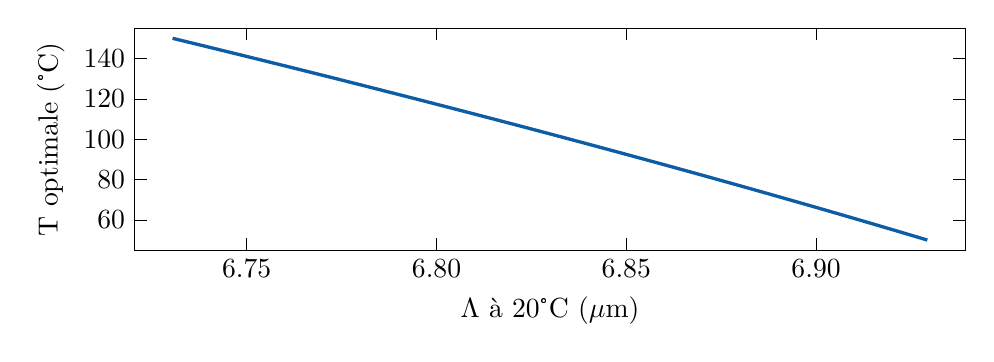
\begin{tikzpicture}

\definecolor{darkgray176}{RGB}{176,176,176}
\definecolor{teal1293165}{RGB}{12,93,165}

\begin{axis}[
width=\linewidth,
height=4.4cm,
tick pos=both,
x grid style={darkgray176},
xlabel={\(\displaystyle \Lambda\) à 20°C (\(\displaystyle \mu\)m)},
xmin=6.72052719717957, xmax=6.93925484373805,
xtick style={color=black},
xtick={6.7,6.75,6.8,6.85,6.9,6.95},
xticklabels={
  \(\displaystyle {6.70}\),
  \(\displaystyle {6.75}\),
  \(\displaystyle {6.80}\),
  \(\displaystyle {6.85}\),
  \(\displaystyle {6.90}\),
  \(\displaystyle {6.95}\)
},
y grid style={darkgray176},
ylabel={T optimale (°C)},
ymin=45, ymax=155,
ytick style={color=black},
ytick={40,60,80,100,120,140,160},
yticklabels={
  \(\displaystyle {40}\),
  \(\displaystyle {60}\),
  \(\displaystyle {80}\),
  \(\displaystyle {100}\),
  \(\displaystyle {120}\),
  \(\displaystyle {140}\),
  \(\displaystyle {160}\)
}
]
\addplot [very thick, teal1293165]
table {%
6.92931267798539 50
6.92895703234664 50.2004008016032
6.9286012069442 50.4008016032064
6.92824520182312 50.6012024048096
6.92788901702851 50.8016032064128
6.92753265260553 51.002004008016
6.92717610859925 51.2024048096192
6.92681938505485 51.4028056112224
6.92646248201755 51.6032064128256
6.92610539953248 51.8036072144289
6.92574813764485 52.0040080160321
6.9253906963998 52.2044088176353
6.92503307584272 52.4048096192385
6.92467527601864 52.6052104208417
6.92431729697291 52.8056112224449
6.92395913875081 53.0060120240481
6.92360080139765 53.2064128256513
6.92324228495854 53.4068136272545
6.92288358947903 53.6072144288577
6.92252471500425 53.8076152304609
6.92216566157971 54.0080160320641
6.92180642925051 54.2084168336673
6.9214470180623 54.4088176352705
6.92108742806025 54.6092184368737
6.92072765928977 54.809619238477
6.92036771179635 55.0100200400802
6.92000758562533 55.2104208416834
6.91964728082215 55.4108216432866
6.91928679743233 55.6112224448898
6.9189261355012 55.811623246493
6.91856529507438 56.0120240480962
6.91820427619722 56.2124248496994
6.9178430789153 56.4128256513026
6.91748170327411 56.6132264529058
6.91712014931913 56.813627254509
6.91675841709599 57.0140280561122
6.9163965066502 57.2144288577154
6.9160344180273 57.4148296593186
6.91567215127285 57.6152304609218
6.91530970643254 57.8156312625251
6.91494708355193 58.0160320641283
6.9145842826766 58.2164328657315
6.91422130385221 58.4168336673347
6.91385814712439 58.6172344689379
6.91349481253887 58.8176352705411
6.91313130014132 59.0180360721443
6.91276760997732 59.2184368737475
6.91240374209268 59.4188376753507
6.91203969653308 59.6192384769539
6.91167547334422 59.8196392785571
6.91131107257187 60.0200400801603
6.91094649426182 60.2204408817635
6.9105817384597 60.4208416833667
6.9102168052114 60.6212424849699
6.90985169456281 60.8216432865731
6.90948640655953 61.0220440881764
6.90912094124751 61.2224448897796
6.90875529867254 61.4228456913828
6.90838947888049 61.623246492986
6.90802348191721 61.8236472945892
6.90765730782858 62.0240480961924
6.90729095666047 62.2244488977956
6.90692442845876 62.4248496993988
6.90655772326947 62.625250501002
6.9061908411384 62.8256513026052
6.90582378211155 63.0260521042084
6.90545654623483 63.2264529058116
6.9050891335543 63.4268537074148
6.90472154411582 63.627254509018
6.90435377796547 63.8276553106212
6.90398583514917 64.0280561122244
6.90361771571299 64.2284569138277
6.90324941970295 64.4288577154309
6.90288094716515 64.6292585170341
6.90251229814557 64.8296593186373
6.90214347269025 65.0300601202405
6.90177447084537 65.2304609218437
6.90140529265695 65.4308617234469
6.90103593817112 65.6312625250501
6.90066640743401 65.8316633266533
6.9002967004917 66.0320641282565
6.89992681739041 66.2324649298597
6.8995567581763 66.4328657314629
6.89918652289545 66.6332665330661
6.89881611159409 66.8336673346693
6.89844552431846 67.0340681362725
6.89807476111471 67.2344689378758
6.89770382202907 67.434869739479
6.89733270710778 67.6352705410822
6.89696141639717 67.8356713426854
6.89658994994333 68.0360721442886
6.8962183077926 68.2364729458918
6.89584648999135 68.436873747495
6.89547449658578 68.6372745490982
6.89510232762221 68.8376753507014
6.89472998314701 69.0380761523046
6.89435746320649 69.2384769539078
6.89398476784697 69.438877755511
6.89361189711482 69.6392785571142
6.89323885105636 69.8396793587174
6.8928656297181 70.0400801603206
6.89249223314637 70.2404809619239
6.89211866138757 70.4408817635271
6.89174491448808 70.6412825651303
6.89137099249441 70.8416833667335
6.89099689545298 71.0420841683367
6.89062262341023 71.2424849699399
6.8902481764126 71.4428857715431
6.88987355450661 71.6432865731463
6.88949875773882 71.8436873747495
6.88912378615562 72.0440881763527
6.88874863980355 72.2444889779559
6.88837331872921 72.4448897795591
6.88799782297903 72.6452905811623
6.88762215259972 72.8456913827655
6.8872463076377 73.0460921843687
6.88687028813962 73.2464929859719
6.88649409415204 73.4468937875751
6.88611772572162 73.6472945891784
6.88574118289489 73.8476953907816
6.88536446571852 74.0480961923848
6.88498757423914 74.248496993988
6.88461050850343 74.4488977955912
6.88423326855806 74.6492985971944
6.88385585444966 74.8496993987976
6.88347826622491 75.0501002004008
6.88310050393056 75.250501002004
6.88272256761324 75.4509018036072
6.88234445731978 75.6513026052104
6.88196617309678 75.8517034068136
6.8815877149911 76.0521042084168
6.88120908304949 76.25250501002
6.88083027731863 76.4529058116233
6.88045129784534 76.6533066132264
6.88007214467649 76.8537074148297
6.8796928178588 77.0541082164329
6.87931331743916 77.2545090180361
6.87893364346424 77.4549098196393
6.87855379598108 77.6553106212425
6.87817377503641 77.8557114228457
6.87779358067707 78.0561122244489
6.87741321295004 78.2565130260521
6.87703267190209 78.4569138276553
6.87665195758018 78.6573146292585
6.87627107003129 78.8577154308617
6.8758900093022 79.0581162324649
6.87550877543994 79.2585170340681
6.8751273684914 79.4589178356713
6.87474578850356 79.6593186372746
6.87436403552333 79.8597194388778
6.87398210959781 80.060120240481
6.87360001077388 80.2605210420842
6.87321773909858 80.4609218436874
6.87283529461892 80.6613226452906
6.87245267738195 80.8617234468938
6.87206988743458 81.062124248497
6.87168692482405 81.2625250501002
6.87130378959722 81.4629258517034
6.87092048180131 81.6633266533066
6.87053700148341 81.8637274549098
6.87015334869048 82.064128256513
6.86976952346967 82.2645290581162
6.86938552586811 82.4649298597194
6.86900135593295 82.6653306613227
6.8686170137113 82.8657314629259
6.86823249925029 83.0661322645291
6.8678478125971 83.2665330661323
6.86746295379888 83.4669338677355
6.86707792290284 83.6673346693387
6.86669271995613 83.8677354709419
6.86630734500604 84.0681362725451
6.86592179809966 84.2685370741483
6.86553607928427 84.4689378757515
6.86515018860714 84.6693386773547
6.86476412611549 84.8697394789579
6.8643778918565 85.0701402805611
6.86399148587754 85.2705410821643
6.8636049082259 85.4709418837675
6.86321815894875 85.6713426853707
6.86283123809359 85.8717434869739
6.86244414570749 86.0721442885772
6.86205688183791 86.2725450901804
6.86166944653223 86.4729458917836
6.86128183983762 86.6733466933868
6.86089406180163 86.87374749499
6.86050611247151 87.0741482965932
6.86011799189465 87.2745490981964
6.85972970011849 87.4749498997996
6.85934123719037 87.6753507014028
6.85895260315774 87.875751503006
6.85856379806794 88.0761523046092
6.85817482196845 88.2765531062124
6.85778567490677 88.4769539078156
6.85739635693023 88.6773547094188
6.85700686808643 88.877755511022
6.85661720842266 89.0781563126253
6.85622737798662 89.2785571142284
6.85583737682564 89.4789579158317
6.85544720498732 89.6793587174349
6.85505686251909 89.8797595190381
6.85466634946855 90.0801603206413
6.85427566588318 90.2805611222445
6.85388481181054 90.4809619238477
6.85349378729822 90.6813627254509
6.85310259239371 90.8817635270541
6.85271122714469 91.0821643286573
6.85231969159866 91.2825651302605
6.8519279858033 91.4829659318637
6.85153610980608 91.6833667334669
6.85114406365479 91.8837675350701
6.85075184739691 92.0841683366733
6.85035946108019 92.2845691382766
6.84996690475219 92.4849699398798
6.84957417846065 92.685370741483
6.84918128225321 92.8857715430862
6.84878821617751 93.0861723446894
6.84839498028129 93.2865731462926
6.84800157461221 93.4869739478958
6.847607999218 93.687374749499
6.8472142541464 93.8877755511022
6.84682033944509 94.0881763527054
6.84642625516182 94.2885771543086
6.84603200134442 94.4889779559118
6.84563757804059 94.689378757515
6.84524298529799 94.8897795591182
6.84484822316462 95.0901803607214
6.84445329168817 95.2905811623247
6.84405819091638 95.4909819639279
6.84366292089717 95.6913827655311
6.84326748167821 95.8917835671343
6.8428718733075 96.0921843687375
6.84247609583277 96.2925851703407
6.8420801493019 96.4929859719439
6.84168403376276 96.6933867735471
6.84128774926325 96.8937875751503
6.84089129585119 97.0941883767535
6.84049467357446 97.2945891783567
6.84009788248105 97.4949899799599
6.83970092261876 97.6953907815631
6.8393037940356 97.8957915831663
6.83890649677943 98.0961923847695
6.83850903089819 98.2965931863727
6.83811139643985 98.496993987976
6.83771359345245 98.6973947895792
6.83731562198378 98.8977955911824
6.836917482082 99.0981963927856
6.83651917379495 99.2985971943888
6.83612069717068 99.498997995992
6.8357220522572 99.6993987975952
6.83532323910259 99.8997995991984
6.83492425775476 100.100200400802
6.83452510826181 100.300601202405
6.83412579067176 100.501002004008
6.8337263050327 100.701402805611
6.83332665139262 100.901803607214
6.8329268297997 101.102204408818
6.83252684030187 101.302605210421
6.83212668294736 101.503006012024
6.83172635778426 101.703406813627
6.83132586486057 101.90380761523
6.83092520422448 102.104208416834
6.83052437592416 102.304609218437
6.83012338000768 102.50501002004
6.82972221652322 102.705410821643
6.82932088551891 102.905811623246
6.82891938704293 103.10621242485
6.82851772114347 103.306613226453
6.82811588786868 103.507014028056
6.82771388726679 103.707414829659
6.82731171938604 103.907815631263
6.82690938427448 104.108216432866
6.82650688198056 104.308617234469
6.82610421255228 104.509018036072
6.82570137603804 104.709418837675
6.82529837248605 104.909819639279
6.82489520194454 105.110220440882
6.82449186446179 105.310621242485
6.82408836008604 105.511022044088
6.82368468886565 105.711422845691
6.82328085084883 105.911823647295
6.82287684608395 106.112224448898
6.82247267461928 106.312625250501
6.82206833650315 106.513026052104
6.82166383178396 106.713426853707
6.82125916050992 106.913827655311
6.82085432272946 107.114228456914
6.82044931849092 107.314629258517
6.82004414784259 107.51503006012
6.81963881083297 107.715430861723
6.8192333075104 107.915831663327
6.81882763792324 108.11623246493
6.81842180211986 108.316633266533
6.81801580014876 108.517034068136
6.8176096320583 108.717434869739
6.81720329789695 108.917835671343
6.81679679771305 109.118236472946
6.81639013155516 109.318637274549
6.81598329947163 109.519038076152
6.81557630151094 109.719438877756
6.81516913772168 109.919839679359
6.81476180815216 110.120240480962
6.81435431285099 110.320641282565
6.81394665186657 110.521042084168
6.81353882524747 110.721442885772
6.81313083304217 110.921843687375
6.8127226752992 111.122244488978
6.81231435206712 111.322645290581
6.81190586339443 111.523046092184
6.81149720932968 111.723446893788
6.81108838992142 111.923847695391
6.81067940521821 112.124248496994
6.81027025526868 112.324649298597
6.80986094012136 112.5250501002
6.80945145982482 112.725450901804
6.80904181442767 112.925851703407
6.8086320039785 113.12625250501
6.80822202852599 113.326653306613
6.80781188811867 113.527054108216
6.80740158280527 113.72745490982
6.80699111263434 113.927855711423
6.80658047765456 114.128256513026
6.80616967791464 114.328657314629
6.80575871346314 114.529058116232
6.80534758434876 114.729458917836
6.80493629062024 114.929859719439
6.8045248323262 115.130260521042
6.80411320951535 115.330661322645
6.80370142223644 115.531062124248
6.80328947053814 115.731462925852
6.80287735446918 115.931863727455
6.80246507407821 116.132264529058
6.80205262941415 116.332665330661
6.80164002052554 116.533066132265
6.80122724746124 116.733466933868
6.80081431027002 116.933867735471
6.80040120900057 117.134268537074
6.79998794370174 117.334669338677
6.79957451442238 117.535070140281
6.79916092121108 117.735470941884
6.79874716411674 117.935871743487
6.79833324318824 118.13627254509
6.79791915847428 118.336673346693
6.79750491002375 118.537074148297
6.79709049788551 118.7374749499
6.79667592210832 118.937875751503
6.79626118274105 119.138276553106
6.79584627983256 119.338677354709
6.7954312134317 119.539078156313
6.7950159835874 119.739478957916
6.79460059034846 119.939879759519
6.79418503376385 120.140280561122
6.79376931388232 120.340681362725
6.79335343075288 120.541082164329
6.79293738442444 120.741482965932
6.7925211749459 120.941883767535
6.79210480236619 121.142284569138
6.79168826673417 121.342685370741
6.79127156809883 121.543086172345
6.79085470650915 121.743486973948
6.79043768201407 121.943887775551
6.79002049466249 122.144288577154
6.78960314450342 122.344689378758
6.78918563158585 122.545090180361
6.78876795595877 122.745490981964
6.78835011767112 122.945891783567
6.78793211677195 123.14629258517
6.78751395331021 123.346693386774
6.78709562733499 123.547094188377
6.78667713889522 123.74749498998
6.78625848803995 123.947895791583
6.78583967481827 124.148296593186
6.78542069927925 124.34869739479
6.78500156147179 124.549098196393
6.78458226144508 124.749498997996
6.78416279924812 124.949899799599
6.78374317492998 125.150300601202
6.78332338853977 125.350701402806
6.7829034401266 125.551102204409
6.78248332973947 125.751503006012
6.78206305742755 125.951903807615
6.78164262323993 126.152304609218
6.78122202722573 126.352705410822
6.78080126943412 126.553106212425
6.78038034991406 126.753507014028
6.7799592687149 126.953907815631
6.7795380258856 127.154308617234
6.77911662147543 127.354709418838
6.77869505553349 127.555110220441
6.77827332810898 127.755511022044
6.77785143925105 127.955911823647
6.77742938900889 128.156312625251
6.77700717743167 128.356713426854
6.77658480456856 128.557114228457
6.77616227046879 128.75751503006
6.77573957518152 128.957915831663
6.77531671875602 129.158316633267
6.7748937012415 129.35871743487
6.77447052268716 129.559118236473
6.77404718314225 129.759519038076
6.77362368265598 129.959919839679
6.77320002127766 130.160320641283
6.77277619905642 130.360721442886
6.77235221604164 130.561122244489
6.77192807228255 130.761523046092
6.77150376782844 130.961923847695
6.77107930272853 131.162324649299
6.77065467703214 131.362725450902
6.77022989078857 131.563126252505
6.76980494404713 131.763527054108
6.76937983685712 131.963927855711
6.76895456926776 132.164328657315
6.7685291413285 132.364729458918
6.76810355308869 132.565130260521
6.76767780459748 132.765531062124
6.76725189590437 132.965931863727
6.7668258270586 133.166332665331
6.76639959810961 133.366733466934
6.76597320910677 133.567134268537
6.76554666009935 133.76753507014
6.76511995113678 133.967935871743
6.76469308226837 134.168336673347
6.7642660535436 134.36873747495
6.76383886501183 134.569138276553
6.76341151672239 134.769539078156
6.76298400872477 134.96993987976
6.76255634106836 135.170340681363
6.76212851380257 135.370741482966
6.76170052697675 135.571142284569
6.76127238064043 135.771543086172
6.76084407484302 135.971943887776
6.76041560963395 136.172344689379
6.75998698506263 136.372745490982
6.75955820117852 136.573146292585
6.75912925803115 136.773547094188
6.7587001556699 136.973947895792
6.75827089414431 137.174348697395
6.75784147350381 137.374749498998
6.7574118937979 137.575150300601
6.75698215507608 137.775551102204
6.75655225738784 137.975951903808
6.75612220078263 138.176352705411
6.75569198531006 138.376753507014
6.75526161101953 138.577154308617
6.75483107796068 138.77755511022
6.75440038618296 138.977955911824
6.75396953573589 139.178356713427
6.75353852666908 139.37875751503
6.75310735903197 139.579158316633
6.75267603287416 139.779559118236
6.75224454824525 139.97995991984
6.75181290519471 140.180360721443
6.75138110377221 140.380761523046
6.75094914402726 140.581162324649
6.75051702600941 140.781563126253
6.75008474976834 140.981963927856
6.74965231535353 141.182364729459
6.74921972281467 141.382765531062
6.74878697220132 141.583166332665
6.74835406356306 141.783567134269
6.74792099694954 141.983967935872
6.74748777241037 142.184368737475
6.74705438999519 142.384769539078
6.74662084975362 142.585170340681
6.74618715173528 142.785571142285
6.74575329598985 142.985971943888
6.74531928256688 143.186372745491
6.74488511151614 143.386773547094
6.74445078288722 143.587174348697
6.74401629672982 143.787575150301
6.74358165309362 143.987975951904
6.74314685202824 144.188376753507
6.74271189358338 144.38877755511
6.74227677780872 144.589178356713
6.74184150475402 144.789579158317
6.74140607446883 144.98997995992
6.74097048700304 145.190380761523
6.74053474240619 145.390781563126
6.74009884072806 145.591182364729
6.73966278201842 145.791583166333
6.73922656632693 145.991983967936
6.73879019370332 146.192384769539
6.73835366419732 146.392785571142
6.73791697785872 146.593186372745
6.73748013473718 146.793587174349
6.7370431348826 146.993987975952
6.73660597834459 147.194388777555
6.73616866517292 147.394789579158
6.73573119541741 147.595190380762
6.73529356912785 147.795591182365
6.73485578635391 147.995991983968
6.73441784714549 148.196392785571
6.73397975155234 148.396793587174
6.73354149962416 148.597194388778
6.73310309141093 148.797595190381
6.73266452696226 148.997995991984
6.73222580632807 149.198396793587
6.73178692955814 149.39879759519
6.73134789670233 149.599198396794
6.73090870781039 149.799599198397
6.73046936293223 150
};
\end{axis}

\end{tikzpicture}

\end{frame}

\section{Discussion}

\begin{frame}{Vérification de la relation $\P_2 = \alpha \P_1^2$ (à \SI{82.5}{\celsius})} 
\centering

% This file was created with tikzplotlib v0.10.1.
\begin{tikzpicture}

\definecolor{darkgray176}{RGB}{176,176,176}
\definecolor{green01270}{RGB}{0,127,0}
\definecolor{teal1293165}{RGB}{12,93,165}

\begin{axis}[
width=\textwidth, height=6cm,
legend cell align={left},
legend style={
	fill=black!2,
  fill opacity=0.8,
  draw opacity=1,
  text opacity=1,
  at={(0.03,0.97)},
  anchor=north west,
  draw=none
},
xlabel={\(\displaystyle \P_1\) ($\unit{mW}$)},
ylabel={\(\displaystyle \P_2\) ($\unit{mW}$)},
tick pos=both,
x grid style={darkgray176},
xmin=-17.5, xmax=367.5,
xtick style={color=black},
y grid style={darkgray176},
ymin=-0.119033690469025, ymax=2.49970749984951,
ytick style={color=black}
]
\path [draw=teal1293165]
(axis cs:166.595,0.565)
--(axis cs:171.255,0.565);

\path [draw=teal1293165]
(axis cs:170.323,0.588)
--(axis cs:174.983,0.588);

\path [draw=teal1293165]
(axis cs:172.187,0.604)
--(axis cs:176.847,0.604);

\path [draw=teal1293165]
(axis cs:65.24,0.104)
--(axis cs:69.9,0.104);

\path [draw=teal1293165]
(axis cs:311.288,1.889)
--(axis cs:315.948,1.889);

\path [draw=teal1293165]
(axis cs:230.204,1.055)
--(axis cs:234.864,1.055);

\path [draw=teal1293165]
(axis cs:236.495,1.12)
--(axis cs:241.155,1.12);

\path [draw=teal1293165]
(axis cs:188.264,0.71)
--(axis cs:192.924,0.71);

\path [draw=teal1293165]
(axis cs:35.649,0.044)
--(axis cs:40.309,0.044);

\path [draw=teal1293165]
(axis cs:85.511,0.161)
--(axis cs:90.171,0.161);

\path [draw=teal1293165]
(axis cs:93.666,0.186)
--(axis cs:98.326,0.186);

\path [draw=teal1293165]
(axis cs:144.926,0.422)
--(axis cs:149.586,0.422);

\path [draw=teal1293165]
(axis cs:168.925,0.545)
--(axis cs:168.925,0.585);

\path [draw=teal1293165]
(axis cs:172.653,0.568)
--(axis cs:172.653,0.608);

\path [draw=teal1293165]
(axis cs:174.517,0.584)
--(axis cs:174.517,0.624);

\path [draw=teal1293165]
(axis cs:67.57,0.084)
--(axis cs:67.57,0.124);

\path [draw=teal1293165]
(axis cs:313.618,1.869)
--(axis cs:313.618,1.909);

\path [draw=teal1293165]
(axis cs:232.534,1.035)
--(axis cs:232.534,1.075);

\path [draw=teal1293165]
(axis cs:238.825,1.1)
--(axis cs:238.825,1.14);

\path [draw=teal1293165]
(axis cs:190.594,0.69)
--(axis cs:190.594,0.73);

\path [draw=teal1293165]
(axis cs:37.979,0.024)
--(axis cs:37.979,0.064);

\path [draw=teal1293165]
(axis cs:87.841,0.141)
--(axis cs:87.841,0.181);

\path [draw=teal1293165]
(axis cs:95.996,0.166)
--(axis cs:95.996,0.206);

\path [draw=teal1293165]
(axis cs:147.256,0.402)
--(axis cs:147.256,0.442);

\addplot [green01270, dashed]
table {%
0 0
0.701402805611222 9.56090059630479e-06
1.40280561122244 3.82436023852192e-05
2.10420841683367 8.60481053667431e-05
2.80561122244489 0.000152974409540877
3.50701402805611 0.00023902251490762
4.20841683366733 0.000344192421466973
4.90981963927856 0.000468484129218935
5.61122244488978 0.000611897638163507
6.312625250501 0.000774432948300688
7.01402805611222 0.00095609005963048
7.71543086172345 0.00115686897215288
8.41683366733467 0.00137676968586789
9.11823647294589 0.00161579220077551
9.81963927855712 0.00187393651687574
10.5210420841683 0.00215120263416858
11.2224448897796 0.00244759055265403
11.9238476953908 0.00276310027233209
12.625250501002 0.00309773179320275
13.3266533066132 0.00345148511526603
14.0280561122244 0.00382436023852192
14.7294589178357 0.00421635716297041
15.4308617234469 0.00462747588861152
16.1322645290581 0.00505771641544524
16.8336673346693 0.00550707874347156
17.5350701402806 0.0059755628726905
18.2364729458918 0.00646316880310204
18.937875751503 0.0069698965347062
19.6392785571142 0.00749574606750296
20.3406813627255 0.00804071740149233
21.0420841683367 0.00860481053667432
21.7434869739479 0.00918802547304891
22.4448897795591 0.00979036221061611
23.1462925851703 0.0104118207493759
23.8476953907816 0.0110524010893283
24.5490981963928 0.0117121032304734
25.250501002004 0.012390927172811
25.9519038076152 0.0130888729163413
26.6533066132265 0.0138059404610641
27.3547094188377 0.0145421298069796
28.0561122244489 0.0152974409540877
28.7575150300601 0.0160718739023884
29.4589178356713 0.0168654286518817
30.1603206412826 0.0176781052025676
30.8617234468938 0.0185099035544461
31.563126252505 0.0193608237075172
32.2645290581162 0.0202308656617809
32.9659318637275 0.0211200294172373
33.6673346693387 0.0220283149738862
34.3687374749499 0.0229557223317278
35.0701402805611 0.023902251490762
35.7715430861723 0.0248679024509888
36.4729458917836 0.0258526752124082
37.1743486973948 0.0268565697750202
37.875751503006 0.0278795861388248
38.5771543086172 0.028921724303822
39.2785571142285 0.0299829842700118
39.9799599198397 0.0310633660373943
40.6813627254509 0.0321628696059693
41.3827655310621 0.033281494975737
42.0841683366734 0.0344192421466973
42.7855711422846 0.0355761111188501
43.4869739478958 0.0367521018921956
44.188376753507 0.0379472144667337
44.8897795591182 0.0391614488424644
45.5911823647295 0.0403948050193878
46.2925851703407 0.0416472829975037
46.9939879759519 0.0429188827768122
47.6953907815631 0.0442096043573134
48.3967935871744 0.0455194477390071
49.0981963927856 0.0468484129218935
49.7995991983968 0.0481964999059725
50.501002004008 0.0495637086912441
51.2024048096192 0.0509500392777082
51.9038076152305 0.0523554916653651
52.6052104208417 0.0537800658542145
53.3066132264529 0.0552237618442565
54.0080160320641 0.0566865796354911
54.7094188376754 0.0581685192279184
55.4108216432866 0.0596695806215382
56.1122244488978 0.0611897638163507
56.813627254509 0.0627290688123558
57.5150300601202 0.0642874956095534
58.2164328657315 0.0658650442079437
58.9178356713427 0.0674617146075266
59.6192384769539 0.0690775068083021
60.3206412825651 0.0707124208102703
61.0220440881764 0.072366456613431
61.7234468937876 0.0740396142177843
62.4248496993988 0.0757318936233303
63.12625250501 0.0774432948300688
63.8276553106212 0.079173817838
64.5290581162325 0.0809234626471238
65.2304609218437 0.0826922292574402
65.9318637274549 0.0844801176689492
66.6332665330661 0.0862871278816508
67.3346693386774 0.088113259895545
68.0360721442886 0.0899585137106318
68.7374749498998 0.0918228893269113
69.438877755511 0.0937063867443833
70.1402805611223 0.095609005963048
70.8416833667335 0.0975307469829052
71.5430861723447 0.0994716098039551
72.2444889779559 0.101431594426198
72.9458917835671 0.103410700849633
73.6472945891784 0.10540892907426
74.3486973947896 0.107426279100081
75.0501002004008 0.109462750927094
75.751503006012 0.111518344555299
76.4529058116233 0.113593059984697
77.1543086172345 0.115686897215288
77.8557114228457 0.117799856247071
78.5571142284569 0.119931937080047
79.2585170340681 0.122083139714216
79.9599198396794 0.124253464149577
80.6613226452906 0.126442910386131
81.3627254509018 0.128651478423877
82.064128256513 0.130879168262816
82.7655310621243 0.133125979902948
83.4669338677355 0.135391913344272
84.1683366733467 0.137676968586789
84.8697394789579 0.139981145630499
85.5711422845691 0.142304444475401
86.2725450901804 0.144646865121495
86.9739478957916 0.147008407568783
87.6753507014028 0.149389071817262
88.376753507014 0.151788857866935
89.0781563126253 0.1542077657178
89.7795591182365 0.156645795369858
90.4809619238477 0.159102946823108
91.1823647294589 0.161579220077551
91.8837675350701 0.164074615133187
92.5851703406814 0.166589131990015
93.2865731462926 0.169122770648036
93.9879759519038 0.171675531107249
94.689378757515 0.174247413367655
95.3907815631263 0.176838417429253
96.0921843687375 0.179448543292045
96.7935871743487 0.182077790956028
97.4949899799599 0.184726160421205
98.1963927855711 0.187393651687574
98.8977955911824 0.190080264755136
99.5991983967936 0.19278599962389
100.300601202405 0.195510856293837
101.002004008016 0.198254834764976
101.703406813627 0.201017935037308
102.404809619238 0.203800157110833
103.10621242485 0.20660150098555
103.807615230461 0.20942196666146
104.509018036072 0.212261554138563
105.210420841683 0.215120263416858
105.911823647295 0.217998094496346
106.613226452906 0.220895047377026
107.314629258517 0.223811122058899
108.016032064128 0.226746318541965
108.717434869739 0.229700636826223
109.418837675351 0.232674076911673
110.120240480962 0.235666638798317
110.821643286573 0.238678322486153
111.523046092184 0.241709127975182
112.224448897796 0.244759055265403
112.925851703407 0.247828104356817
113.627254509018 0.250916275249423
114.328657314629 0.254023567943222
115.03006012024 0.257149982438214
115.731462925852 0.260295518734398
116.432865731463 0.263460176831775
117.134268537074 0.266643956730344
117.835671342685 0.269846858430106
118.537074148297 0.273068881931061
119.238476953908 0.276310027233209
119.939879759519 0.279570294336549
120.64128256513 0.282849683241081
121.342685370741 0.286148193946806
122.044088176353 0.289465826453724
122.745490981964 0.292802580761834
123.446893787575 0.296158456871137
124.148296593186 0.299533454781633
124.849699398798 0.302927574493321
125.551102204409 0.306340816006202
126.25250501002 0.309773179320275
126.953907815631 0.313224664435541
127.655310621242 0.316695271352
128.356713426854 0.320185000069651
129.058116232465 0.323693850588495
129.759519038076 0.327221822908532
130.460921843687 0.330768917029761
131.162324649299 0.334335132952182
131.86372745491 0.337920470675797
132.565130260521 0.341524930200604
133.266533066132 0.345148511526603
133.967935871743 0.348791214653795
134.669338677355 0.35245303958218
135.370741482966 0.356133986311757
136.072144288577 0.359834054842527
136.773547094188 0.36355324517449
137.4749498998 0.367291557307645
138.176352705411 0.371048991241993
138.877755511022 0.374825546977533
139.579158316633 0.378621224514266
140.280561122245 0.382436023852192
140.981963927856 0.38626994499131
141.683366733467 0.390122987931621
142.384769539078 0.393995152673124
143.086172344689 0.39788643921582
143.787575150301 0.401796847559709
144.488977955912 0.40572637770479
145.190380761523 0.409675029651064
145.891783567134 0.413642803398531
146.593186372745 0.41762969894719
147.294589178357 0.421635716297041
147.995991983968 0.425660855448086
148.697394789579 0.429705116400323
149.39879759519 0.433768499153752
150.100200400802 0.437851003708374
150.801603206413 0.441952630064189
151.503006012024 0.446073378221197
152.204408817635 0.450213248179397
152.905811623247 0.454372239938789
153.607214428858 0.458550353499374
154.308617234469 0.462747588861152
155.01002004008 0.466963946024123
155.711422845691 0.471199424988286
156.412825651303 0.475454025753641
157.114228456914 0.479727748320189
157.815631262525 0.48402059268793
158.517034068136 0.488332558856864
159.218436873747 0.49266364682699
159.919839679359 0.497013856598308
160.62124248497 0.50138318817082
161.322645290581 0.505771641544524
162.024048096192 0.51017921671942
162.725450901804 0.514605913695509
163.426853707415 0.519051732472791
164.128256513026 0.523516673051265
164.829659318637 0.528000735430932
165.531062124249 0.532503919611792
166.23246492986 0.537026225593844
166.933867735471 0.541567653377089
167.635270541082 0.546128202961526
168.336673346693 0.550707874347156
169.038076152305 0.555306667533979
169.739478957916 0.559924582521994
170.440881763527 0.564561619311202
171.142284569138 0.569217777901602
171.84368737475 0.573893058293195
172.545090180361 0.578587460485981
173.246492985972 0.583300984479959
173.947895791583 0.58803363027513
174.649298597194 0.592785397871494
175.350701402806 0.59755628726905
176.052104208417 0.602346298467798
176.753507014028 0.60715543146774
177.454909819639 0.611983686268874
178.156312625251 0.6168310628712
178.857715430862 0.621697561274719
179.559118236473 0.626583181479431
180.260521042084 0.631487923485335
180.961923847695 0.636411787292432
181.663326653307 0.641354772900722
182.364729458918 0.646316880310204
183.066132264529 0.651298109520879
183.76753507014 0.656298460532746
184.468937875752 0.661317933345806
185.170340681363 0.666356527960059
185.871743486974 0.671414244375504
186.573146292585 0.676491082592142
187.274549098196 0.681587042609972
187.975951903808 0.686702124428995
188.677354709419 0.691836328049211
189.37875751503 0.696989653470619
190.080160320641 0.70216210069322
190.781563126253 0.707353669717014
191.482965931864 0.712564360542
192.184368737475 0.717794173168179
192.885771543086 0.72304310759555
193.587174348697 0.728311163824114
194.288577154309 0.733598341853871
194.98997995992 0.73890464168482
195.691382765531 0.744230063316962
196.392785571142 0.749574606750296
197.094188376754 0.754938271984823
197.795591182365 0.760321059020543
198.496993987976 0.765722967857455
199.198396793587 0.77114399849556
199.899799599198 0.776584150934857
200.60120240481 0.782043425175347
201.302605210421 0.78752182121703
202.004008016032 0.793019339059905
202.705410821643 0.798535978703973
203.406813627255 0.804071740149233
204.108216432866 0.809626623395686
204.809619238477 0.815200628443332
205.511022044088 0.82079375529217
206.212424849699 0.826406003942201
206.913827655311 0.832037374393425
207.615230460922 0.837687866645841
208.316633266533 0.84335748069945
209.018036072144 0.849046216554251
209.719438877756 0.854754074210245
210.420841683367 0.860481053667432
211.122244488978 0.866227154925811
211.823647294589 0.871992377985383
212.5250501002 0.877776722846147
213.226452905812 0.883580189508104
213.927855711423 0.889402777971254
214.629258517034 0.895244488235596
215.330661322645 0.901105320301131
216.032064128257 0.906985274167858
216.733466933868 0.912884349835778
217.434869739479 0.918802547304891
218.13627254509 0.924739866575196
218.837675350701 0.930696307646694
219.539078156313 0.936671870519384
220.240480961924 0.942666555193267
220.941883767535 0.948680361668343
221.643286573146 0.954713289944612
222.344689378758 0.960765340022072
223.046092184369 0.966836511900726
223.74749498998 0.972926805580572
224.448897795591 0.979036221061611
225.150300601202 0.985164758343842
225.851703406814 0.991312417427266
226.553106212425 0.997479198311883
227.254509018036 1.00366510099769
227.955911823647 1.00987012548469
228.657314629259 1.01609427177289
229.35871743487 1.02233753986228
230.060120240481 1.02859992975286
230.761523046092 1.03488144144463
231.462925851703 1.04118207493759
232.164328657315 1.04750183023175
232.865731462926 1.0538407073271
233.567134268537 1.06019870622364
234.268537074148 1.06657582692138
234.96993987976 1.07297206942031
235.671342685371 1.07938743372043
236.372745490982 1.08582191982174
237.074148296593 1.09227552772425
237.775551102204 1.09874825742794
238.476953907816 1.10524010893283
239.178356713427 1.11175108223892
239.879759519038 1.11828117734619
240.581162324649 1.12483039425466
241.282565130261 1.13139873296432
241.983967935872 1.13798619347518
242.685370741483 1.14459277578722
243.386773547094 1.15121847990046
244.088176352705 1.1578633058149
244.789579158317 1.16452725353052
245.490981963928 1.17121032304734
246.192384769539 1.17791251436535
246.89378757515 1.18463382748455
247.595190380762 1.19137426240494
248.296593186373 1.19813381912653
248.997995991984 1.20491249764931
249.699398797595 1.21171029797328
250.400801603206 1.21852722009845
251.102204408818 1.22536326402481
251.803607214429 1.23221842975236
252.50501002004 1.2390927172811
253.206412825651 1.24598612661104
253.907815631263 1.25289865774217
254.609218436874 1.25983031067449
255.310621242485 1.266781085408
256.012024048096 1.27375098194271
256.713426853707 1.2807400002786
257.414829659319 1.2877481404157
258.11623246493 1.29477540235398
258.817635270541 1.30182178609346
259.519038076152 1.30888729163413
260.220440881764 1.31597191897599
260.921843687375 1.32307566811904
261.623246492986 1.33019853906329
262.324649298597 1.33734053180873
263.026052104208 1.34450164635536
263.72745490982 1.35168188270319
264.428857715431 1.3588812408522
265.130260521042 1.36609972080241
265.831663326653 1.37333732255382
266.533066132265 1.38059404610641
267.234468937876 1.3878698914602
267.935871743487 1.39516485861518
268.637274549098 1.40247894757135
269.338677354709 1.40981215832872
270.040080160321 1.41716449088728
270.741482965932 1.42453594524703
271.442885771543 1.43192652140797
272.144288577154 1.43933621937011
272.845691382766 1.44676503913344
273.547094188377 1.45421298069796
274.248496993988 1.46168004406367
274.949899799599 1.46916622923058
275.65130260521 1.47667153619868
276.352705410822 1.48419596496797
277.054108216433 1.49173951553846
277.755511022044 1.49930218791013
278.456913827655 1.506883982083
279.158316633267 1.51448489805706
279.859719438878 1.52210493583232
280.561122244489 1.52974409540877
281.2625250501 1.53740237678641
281.963927855711 1.54507977996524
282.665330661323 1.55277630494527
283.366733466934 1.56049195172648
284.068136272545 1.56822672030889
284.769539078156 1.5759806106925
285.470941883768 1.58375362287729
286.172344689379 1.59154575686328
286.87374749499 1.59935701265046
287.575150300601 1.60718739023884
288.276553106212 1.6150368896284
288.977955911824 1.62290551081916
289.679358717435 1.63079325381111
290.380761523046 1.63870011860426
291.082164328657 1.64662610519859
291.783567134269 1.65457121359412
292.48496993988 1.66253544379084
293.186372745491 1.67051879578876
293.887775551102 1.67852126958787
294.589178356713 1.68654286518817
295.290581162325 1.69458358258966
295.991983967936 1.70264342179234
296.693386773547 1.71072238279622
297.394789579158 1.71882046560129
298.09619238477 1.72693767020755
298.797595190381 1.73507399661501
299.498997995992 1.74322944482366
300.200400801603 1.7514040148335
300.901803607214 1.75959770664453
301.603206412826 1.76781052025676
302.304609218437 1.77604245567018
303.006012024048 1.78429351288479
303.707414829659 1.79256369190059
304.408817635271 1.80085299271759
305.110220440882 1.80916141533578
305.811623246493 1.81748895975516
306.513026052104 1.82583562597573
307.214428857715 1.8342014139975
307.915831663327 1.84258632382046
308.617234468938 1.85099035544461
309.318637274549 1.85941350886995
310.02004008016 1.86785578409649
310.721442885772 1.87631718112422
311.422845691383 1.88479769995314
312.124248496994 1.89329734058326
312.825651302605 1.90181610301457
313.527054108216 1.91035398724707
314.228456913828 1.91891099328076
314.929859719439 1.92748712111564
315.63126252505 1.93608237075172
316.332665330661 1.94469674218899
317.034068136273 1.95333023542745
317.735470941884 1.96198285046711
318.436873747495 1.97065458730796
319.138276553106 1.97934544595
319.839679358717 1.98805542639323
320.541082164329 1.99678452863766
321.24248496994 2.00553275268328
321.943887775551 2.01430009853009
322.645290581162 2.02308656617809
323.346693386774 2.03189215562729
324.048096192385 2.04071686687768
324.749498997996 2.04956069992926
325.450901803607 2.05842365478204
326.152304609218 2.067305731436
326.85370741483 2.07620692989116
327.555110220441 2.08512725014752
328.256513026052 2.09406669220506
328.957915831663 2.1030252560638
329.659318637275 2.11200294172373
330.360721442886 2.12099974918485
331.062124248497 2.13001567844717
331.763527054108 2.13905072951068
332.464929859719 2.14810490237538
333.166332665331 2.15717819704127
333.867735470942 2.16627061350836
334.569138276553 2.17538215177663
335.270541082164 2.1845128118461
335.971943887776 2.19366259371677
336.673346693387 2.20283149738862
337.374749498998 2.21201952286167
338.076152304609 2.22122667013592
338.77755511022 2.23045293921135
339.478957915832 2.23969833008798
340.180360721443 2.2489628427658
340.881763527054 2.25824647724481
341.583166332665 2.26754923352501
342.284569138277 2.27687111160641
342.985971943888 2.286212111489
343.687374749499 2.29557223317278
344.38877755511 2.30495147665776
345.090180360721 2.31434984194392
345.791583166333 2.32376732903128
346.492985971944 2.33320393791984
347.194388777555 2.34265966860958
347.895791583166 2.35213452110052
348.597194388778 2.36162849539265
349.298597194389 2.37114159148597
350 2.38067380938049
};
\addlegendentry{$\alpha=\SI{1.9}{\percent\per\watt}$}
\addplot [teal1293165, mark=*, mark size=1.5, mark options={solid}, only marks, forget plot]
table {%
168.925 0.565
172.653 0.588
174.517 0.604
67.57 0.104
313.618 1.889
232.534 1.055
238.825 1.12
190.594 0.71
37.979 0.044
87.841 0.161
95.996 0.186
147.256 0.422
};
\end{axis}

\end{tikzpicture}
\end{frame}

\begin{frame}{Dépendance en température de l'efficacité de conversion}
\centering
% This file was created with tikzplotlib v0.10.1.
\begin{tikzpicture}

\definecolor{darkgray176}{RGB}{176,176,176}
\definecolor{green01270}{RGB}{0,127,0}
\definecolor{teal1293165}{RGB}{12,93,165}

\begin{axis}[
width=\textwidth, height=6cm,
legend cell align={left},
legend style={fill=black!2,fill opacity=0.8, draw opacity=1, text opacity=1, at={(1,0.7)}, anchor=north east, draw=none},
tick pos=both,
x grid style={darkgray176},
xlabel={\(\displaystyle T\) ($\unit{\celsius}$)},
xmin=74, xmax=96,
xtick style={color=black},
y grid style={darkgray176},
ylabel={\(\displaystyle \alpha\) ($\unit{\percent\per\watt}$)},
ymin=-0.2824956269314, ymax=3.78741939120156,
ytick style={color=black}
]
\path [draw=teal1293165]
(axis cs:77.95,0.00760714010396571)
--(axis cs:78.05,0.00760714010396571);

\path [draw=teal1293165]
(axis cs:79.95,0.0083288727592556)
--(axis cs:80.05,0.0083288727592556);

\path [draw=teal1293165]
(axis cs:81.95,0.339120757203844)
--(axis cs:82.05,0.339120757203844);

\path [draw=teal1293165]
(axis cs:82.25,1.53475334684663)
--(axis cs:82.35,1.53475334684663);

\path [draw=teal1293165]
(axis cs:82.45,2.66026813240154)
--(axis cs:82.55,2.66026813240154);

\path [draw=teal1293165]
(axis cs:82.75,2.71784755564717)
--(axis cs:82.85,2.71784755564717);

\path [draw=teal1293165]
(axis cs:82.95,3.07568000803268)
--(axis cs:83.05,3.07568000803268);

\path [draw=teal1293165]
(axis cs:83.05,2.88265306122449)
--(axis cs:83.15,2.88265306122449);

\path [draw=teal1293165]
(axis cs:83.15,3.19720403201938)
--(axis cs:83.25,3.19720403201938);

\path [draw=teal1293165]
(axis cs:83.25,3.41687059190433)
--(axis cs:83.35,3.41687059190433);

\path [draw=teal1293165]
(axis cs:83.35,3.17743475662863)
--(axis cs:83.45,3.17743475662863);

\path [draw=teal1293165]
(axis cs:83.45,3.163737512112)
--(axis cs:83.55,3.163737512112);

\path [draw=teal1293165]
(axis cs:83.55,3.08984255353263)
--(axis cs:83.65,3.08984255353263);

\path [draw=teal1293165]
(axis cs:83.65,2.7810650887574)
--(axis cs:83.75,2.7810650887574);

\path [draw=teal1293165]
(axis cs:83.75,2.01736880063011)
--(axis cs:83.85,2.01736880063011);

\path [draw=teal1293165]
(axis cs:83.95,2.05631896971249)
--(axis cs:84.05,2.05631896971249);

\path [draw=teal1293165]
(axis cs:84.15,0.777541534378738)
--(axis cs:84.25,0.777541534378738);

\path [draw=teal1293165]
(axis cs:84.95,0.0131710583679215)
--(axis cs:85.05,0.0131710583679215);

\path [draw=teal1293165]
(axis cs:85.95,0.0519206741986608)
--(axis cs:86.05,0.0519206741986608);

\path [draw=teal1293165]
(axis cs:86.95,0.0537923614846692)
--(axis cs:87.05,0.0537923614846692);

\path [draw=teal1293165]
(axis cs:89.95,0.0105337228497396)
--(axis cs:90.05,0.0105337228497396);

\path [draw=teal1293165]
(axis cs:78,-0.02594758676084)
--(axis cs:78,0.0411618669687714);

\path [draw=teal1293165]
(axis cs:80,-0.0974994897435382)
--(axis cs:80,0.114157235262049);

\path [draw=teal1293165]
(axis cs:82,0.312675825494948)
--(axis cs:82,0.365565688912741);

\path [draw=teal1293165]
(axis cs:82.3,1.48683781677571)
--(axis cs:82.3,1.58266887691755);

\path [draw=teal1293165]
(axis cs:82.5,2.38897394724412)
--(axis cs:82.5,2.93156231755896);

\path [draw=teal1293165]
(axis cs:82.8,2.65849342178912)
--(axis cs:82.8,2.77720168950522);

\path [draw=teal1293165]
(axis cs:83,2.81296685133931)
--(axis cs:83,3.33839316472606);

\path [draw=teal1293165]
(axis cs:83.1,2.61993990453112)
--(axis cs:83.1,3.14536621791786);

\path [draw=teal1293165]
(axis cs:83.2,3.130519243065)
--(axis cs:83.2,3.26388882097375);

\path [draw=teal1293165]
(axis cs:83.3,3.23131792979496)
--(axis cs:83.3,3.6024232540137);

\path [draw=teal1293165]
(axis cs:83.4,3.09631552297269)
--(axis cs:83.4,3.25855399028457);

\path [draw=teal1293165]
(axis cs:83.5,3.08261827845606)
--(axis cs:83.5,3.24485674576794);

\path [draw=teal1293165]
(axis cs:83.6,2.79895814249604)
--(axis cs:83.6,3.38072696456922);

\path [draw=teal1293165]
(axis cs:83.7,2.49018067772081)
--(axis cs:83.7,3.07194949979399);

\path [draw=teal1293165]
(axis cs:83.8,2.01327339933101)
--(axis cs:83.8,2.02146420192922);

\path [draw=teal1293165]
(axis cs:84,1.27096627044354)
--(axis cs:84,2.84167166898143);

\path [draw=teal1293165]
(axis cs:84.2,0.769325483184936)
--(axis cs:84.2,0.785757585572539);

\path [draw=teal1293165]
(axis cs:85,-0.00447329449266556)
--(axis cs:85,0.0308154112285085);

\path [draw=teal1293165]
(axis cs:86,0.0331444854992324)
--(axis cs:86,0.0706968628980893);

\path [draw=teal1293165]
(axis cs:87,0.0350161727852407)
--(axis cs:87,0.0725685501840977);

\path [draw=teal1293165]
(axis cs:90,-0.0015610376072696)
--(axis cs:90,0.0226284833067489);

\addplot [green01270, dashed]
table {%
75 0.0143320321968209
75.0400801603206 0.0138762434343119
75.0801603206413 0.0132972301699636
75.1202404809619 0.0126047115114497
75.1603206412826 0.0118107173532076
75.2004008016032 0.0109294140018178
75.2404809619239 0.00997688733749785
75.2805611222445 0.00897088661032758
75.3206412825651 0.00793053274105297
75.3607214428858 0.00687599571297853
75.4008016032064 0.00582814628971591
75.4408817635271 0.00480818786054282
75.4809619238477 0.0038372746891673
75.5210420841683 0.00293612321254993
75.561122244489 0.00212462329550469
75.6012024048096 0.00142145648729145
75.6412825651303 0.000843728343515821
75.6813627254509 0.000406621767645617
75.7214428857715 0.000123078090782675
75.7615230460922 3.51224770680857e-06
75.8016032064128 5.55679255377673e-05
75.8416833667335 0.000283917964806329
75.8817635270541 0.000690114589574195
75.9218436873747 0.00127249324383515
75.9619238476954 0.00202613292800901
76.002004008016 0.00294287497587048
76.0420841683367 0.00401140120421498
76.0821643286573 0.00521737132169891
76.122244488978 0.00654361841735332
76.1623246492986 0.00797040028171424
76.2024048096192 0.00947570326320169
76.2424849699399 0.0110355943482491
76.2825651302605 0.0126246161944285
76.3226452905812 0.0142162189595355
76.3627254509018 0.0157832219735016
76.4028056112224 0.017298297610044
76.4428857715431 0.0187344691456088
76.4829659318637 0.0200656139570263
76.5230460921844 0.0212669631169416
76.563126252505 0.02231558830579
76.6032064128257 0.0231908669766237
76.6432865731463 0.0238749168876232
76.6833667334669 0.024352991457051
76.7234468937876 0.024613827894314
76.7635270541082 0.0246499407134862
76.8036072144289 0.024457854034076
76.8436873747495 0.0240382670072808
76.8837675350701 0.0233961477611479
76.9238476953908 0.0225407524192387
76.9639278557114 0.0214855669966699
77.0040080160321 0.0202481712949659
77.0440881763527 0.0188500252815351
77.0841683366733 0.0173161798280767
77.124248496994 0.0156749150711324
77.1643286573146 0.0139573110231711
77.2044088176353 0.0121967563796524
77.2444889779559 0.0104284027124544
77.2845691382766 0.00868857238947641
77.3246492985972 0.00701412959193231
77.3647294589178 0.00544182469408885
77.4048096192385 0.00400762300617205
77.4448897795591 0.00274602944330634
77.4849699398798 0.00168942105771565
77.5250501002004 0.00086739954695058
77.565130260521 0.000306175819696457
77.6052104208417 2.79984582129011e-05
77.6452905811623 5.06374615964418e-05
77.685370741483 0.000386933989395837
77.7254509018036 0.00104442595682786
77.7655310621243 0.00202505827074189
77.8056112224449 0.00332498525289846
77.8456913827655 0.00493447139078249
77.8857715430862 0.00683789500597308
77.9258517034068 0.00901385775886215
77.9659318637274 0.0114354011416996
78.0060120240481 0.0140703292771811
78.0460921843687 0.0168816354666535
78.0861723446894 0.0198280280512682
78.12625250501 0.0228645492929283
78.1663326653307 0.0259432791817313
78.2064128256513 0.0290141143648473
78.2464929859719 0.0320256107997006
78.2865731462926 0.0349258772920586
78.3266533066132 0.0376635058155405
78.3667334669339 0.0401885234492506
78.4068136272545 0.0424533499380945
78.4468937875751 0.0444137442960313
78.4869739478958 0.0460297235526431
78.5270541082164 0.0472664367005943
78.5671342685371 0.0480949771441877
78.6072144288577 0.0484931174811748
78.6472945891784 0.0484459512704662
78.687374749499 0.0479464275418692
78.7274549098196 0.0469957651800959
78.7675350701403 0.0456037359489989
78.8076152304609 0.0437888067935939
78.8476953907816 0.0415781341428806
78.8877755511022 0.0390074052075794
78.9278557114229 0.0361205236917415
78.9679358717435 0.0329691398805012
79.0080160320641 0.0296120276899174
79.0480961923848 0.0261143139285016
79.0881763527054 0.0225465676815494
79.1282565130261 0.0189837603455784
79.1683366733467 0.0155041093675038
79.2084168336673 0.0121878211381725
79.248496993988 0.00911575071047495
79.2885771543086 0.00636799801735637
79.3286573146293 0.00402246201673276
79.3687374749499 0.00215337565292176
79.4088176352705 0.000829845666187176
79.4488977955912 0.000114422075817376
79.4889779559118 6.17225850764128e-05
79.5290581162325 0.000717137190860447
79.5691382765531 0.00211563791503999
79.6092184368737 0.00428071780228643
79.6492985971944 0.00722348215084236
79.689378757515 0.0109419133646778
79.7294589178357 0.0154203288506006
79.7695390781563 0.0206290490512864
79.809619238477 0.0265242900301297
79.8496993987976 0.0330482920374733
79.8897795591182 0.0401296922268743
79.9298597194389 0.0476841461964902
79.9699398797595 0.0556151993508612
80.0100200400802 0.063815405262815
80.0501002004008 0.0721676843177012
80.0901803607214 0.0805469119990772
80.1302605210421 0.0888217222844571
80.1703406813627 0.0968565078209695
80.2104208416834 0.104513594902921
80.250501002004 0.111655567834795
80.2905811623247 0.118147714090838
80.3306613226453 0.123860558830207
80.3707414829659 0.128672454845661
80.4108216432866 0.132472191959897
80.4509018036072 0.135161588279089
80.4909819639279 0.136658024602894
80.5310621242485 0.136896882703991
80.5711422845691 0.135833848150171
80.6112224448898 0.133447038863147
80.6513026052104 0.129738921697586
80.6913827655311 0.124737980980644
80.7314629258517 0.118500105167137
80.7715430861723 0.111109660521246
80.811623246493 0.102680224006764
80.8517034068136 0.093354951320893
80.8917835671343 0.0833065602006081
80.9318637274549 0.0727369137173967
80.9719438877756 0.0618761932011058
81.0120240480962 0.0509816556360592
81.0521042084168 0.0403359757867715
81.0921843687375 0.0302451788664404
81.1322645290581 0.021036175185481
81.1723446893788 0.0130539138338638
81.2124248496994 0.00665817798271798
81.25250501002 0.00222004976011716
81.2925851703407 0.000118077786471679
81.3326653306613 0.000734185271767872
81.372745490982 0.00444936100820294
81.4128256513026 0.0116391795698249
81.4529058116233 0.0226692004929149
81.4929859719439 0.0378902991001979
81.5330661322645 0.0576339838991516
81.5731462925852 0.0822077570866958
81.6132264529058 0.111890575596885
81.6533066132264 0.146928470308767
81.6933867735471 0.187530380473963
81.7334669338677 0.233864259121651
81.7735470941884 0.286053503157016
81.813627254509 0.344173759102378
81.8537074148297 0.40825015196237
81.8937875751503 0.478254980560078
81.9338677354709 0.554105917933401
81.9739478957916 0.635664750052634
82.0140280561122 0.722736680282273
82.0541082164329 0.815070220730581
82.0941883767535 0.912357684984767
82.1342685370741 1.01423628979855
82.1743486973948 1.12028986616798
82.2144288577154 1.23005117299
82.2545090180361 1.34300479923783
82.2945891783567 1.45859063340111
82.3346693386774 1.57620787191881
82.374749498998 1.69521953157225
82.4148296593186 1.8149574243913
82.4549098196393 1.93472754764597
82.4949899799599 2.05381583602727
82.5350701402806 2.17149421824042
82.5751503006012 2.2870269160067
82.6152304609219 2.3996769199575
82.6553106212425 2.50871257415477
82.6953907815631 2.61341419902756
82.7354709418838 2.71308068140363
82.7755511022044 2.80703596006091
82.815631262525 2.89463533583018
82.8557114228457 2.97527153674959
82.8957915831663 3.04838047108727
82.935871743487 3.11344660418618
82.9759519038076 3.17000789901078
83.0160320641283 3.2176602649411
83.0561122244489 3.25606146471157
83.0961923847695 3.2849344353649
83.1362725450902 3.30406998561194
83.1763527054108 3.31332883897766
83.2164328657315 3.31264299948369
83.2565130260521 3.30201642427929
83.2965931863727 3.2815249954886
83.3366733466934 3.25131579149587
83.376753507014 3.21160566584173
83.4168336673347 3.16267914975509
83.4569138276553 3.10488570199692
83.496993987976 3.03863633705093
83.5370741482966 2.96439966966925
83.5771543086172 2.88269742028347
83.6172344689379 2.7940994317418
83.6573146292585 2.69921825316049
83.6973947895792 2.59870335131589
83.7374749498998 2.49323501389863
83.7775551102204 2.38351801205686
83.8176352705411 2.27027509193761
83.8577154308617 2.15424036636545
83.8977955911824 2.03615267837117
83.937875751503 1.9167490079843
83.9779559118236 1.79675799255819
84.0180360721443 1.67689362890712
84.0581162324649 1.55784922274751
84.0981963927856 1.44029164738099
84.1382765531062 1.32485596929021
84.1783567134269 1.21214049339841
84.2184368737475 1.1027022752372
84.2585170340681 0.997053141249037
84.2985971943888 0.895656252002295
84.3386773547094 0.798923236302663
84.3787575150301 0.707211917134744
84.4188376753507 0.620824643153516
84.4589178356713 0.540007232160268
84.498997995992 0.464948525734552
84.5390781563126 0.395780547044677
84.5791583166333 0.332579246913554
84.6192384769539 0.275365816560207
84.6593186372746 0.224108539150897
84.6993987975952 0.178725146452813
84.7394789579158 0.139085641556117
84.7795591182365 0.10501554387766
84.8196392785571 0.0762995085343077
84.8597194388778 0.0526852687192026
84.8997995991984 0.0338878469644007
84.939879759519 0.0195939791524222
84.9799599198397 0.00946669386189397
85.0200400801603 0.00314998910201686
85.060120240481 0.000273548702646427
85.1002004008016 0.000457441563804058
85.1402805611222 0.00331674860722073
85.1803607214429 0.00846606457743628
85.2204408817635 0.0155238247695187
85.2605210420842 0.0241164102638824
85.3006012024048 0.0338819892690919
85.3406813627254 0.0444740566477327
85.3807615230461 0.055564638560239
85.4208416833667 0.0668471343347596
85.4609218436874 0.0780387730824962
85.501002004008 0.0888826681503739
85.5410821643287 0.0991494581584781
85.5811623246493 0.108638529030837
85.6212424849699 0.117178817018607
85.6613226452906 0.124629198160716
85.7014028056112 0.130878474858161
85.7414829659319 0.13584497518835
85.7815631262525 0.139475785194215
85.8216432865731 0.141745638594475
85.8617234468938 0.142655492127937
85.9018036072144 0.142230818025059
85.9418837675351 0.140519647860668
85.9819639278557 0.137590404257077
86.0220440881764 0.13352955855971
86.062124248497 0.128439153688455
86.1022044088176 0.122434231876669
86.1422845691383 0.115640206953166
86.1823647294589 0.108190220215887
86.2224448897796 0.100222517811803
86.2625250501002 0.0918778859053915
86.3026052104208 0.0832971778241961
86.3426853707415 0.0746189648556691
86.3827655310621 0.0659773394822841
86.4228456913828 0.0574998966324229
86.4629258517034 0.0493059150476607
86.503006012024 0.0415047571798948
86.5430861723447 0.0341945021932005
86.5831663326653 0.027460822715023
86.623246492986 0.021376112018946
86.6633266533066 0.015998864385432
86.7034068136273 0.0113733075344462
86.7434869739479 0.00752928230897252
86.7835671342685 0.00448236126197883
86.8236472945892 0.00223419450823197
86.8637274549098 0.0007730681887001
86.9038076152305 7.4658196148647e-05
86.9438877755511 0.000102959457372097
86.9839679358717 0.000811369085788921
87.0240480961924 0.0021439001271536
87.064128256513 0.00403650143384416
87.1042084168337 0.00641845842610758
87.1442885771543 0.00921384913197342
87.184368737475 0.0123430299352496
87.2244488977956 0.015724125891087
87.2645290581162 0.0192745012733687
87.3046092184369 0.0229121871747123
87.3446893787575 0.0265572444604571
87.3847695390781 0.030133042150595
87.4248496993988 0.03356743333271
87.4649298597194 0.0367938129556008
87.5050100200401 0.0397520442767441
87.5450901803607 0.0423892432939286
87.5851703406814 0.0446604131388314
87.625250501002 0.046528923103838
87.6653306613226 0.0479668296694627
87.7054108216433 0.0489550395557642
87.7454909819639 0.049483317396337
87.7855711422846 0.0495501430892821
87.8256513026052 0.049162426180358
87.8657314629259 0.0483350867469819
87.9058116232465 0.0470905141493585
87.9458917835671 0.0454579166723884
87.9859719438878 0.0434725764791793
88.0260521042084 0.0411750254186552
88.0661322645291 0.038610158065384
88.1062124248497 0.0358262989136262
88.1462925851703 0.0328742408988519
88.186372745491 0.0298062723824065
88.2264529058116 0.0266752094169773
88.2665330661323 0.0235334495247174
88.3066132264529 0.0204320623829578
88.3466933867736 0.0174199317447279
88.3867735470942 0.0145429616463236
88.4268537074148 0.0118433584982534
88.4669338677355 0.00935899904765444
88.5070140280561 0.00712289247009048
88.5470941883767 0.00516274302818286
88.5871743486974 0.00350061785601466
88.627254509018 0.00215272252437945
88.6673346693387 0.00112928514457503
88.7074148296593 0.000434547909074553
88.74749498998 6.68631757133984e-05
88.7875751503006 1.888950615166e-05
88.8276553106212 0.000277881495055572
88.8677354709419 0.000826065796867993
88.9078156312625 0.00164109449243399
88.9478957915832 0.00269656585513537
88.9879759519038 0.00396260168917518
89.0280561122244 0.00540646973128136
89.0681362725451 0.00699323913776292
89.1082164328657 0.00868645682427112
89.1482965931864 0.0104488323848686
89.188376753507 0.0122429194856298
89.2284569138277 0.0140317819981295
89.2685370741483 0.015779633698774
89.3086172344689 0.017452441097017
89.3486973947896 0.0190184798524557
89.3887775551102 0.0204488362786996
89.4288577154309 0.0217178465898781
89.4689378757515 0.0228034678012907
89.5090180360721 0.0236875755254448
89.5490981963928 0.0243561852842855
89.5891783567134 0.0247995953632225
89.6292585170341 0.0250124506381226
89.6693386773547 0.0249937281888217
89.7094188376753 0.0247466468488922
89.749498997996 0.0242785041096238
89.7895791583166 0.0236004449763289
89.8296593186373 0.0227271684489553
89.8697394789579 0.021676578250599
89.9098196392786 0.0204693852432578
89.9498997995992 0.0191286696390878
89.9899799599198 0.0176794116292589
90.0300601202405 0.016147999405828
90.0701402805611 0.0145617237422704
90.1102204408818 0.0129482683256899
90.1503006012024 0.0113352049012958
90.190380761523 0.00974950200318726
90.2304609218437 0.00821705561303639
90.2705410821643 0.00676224952046026
90.310621242485 0.00540755246835836
90.3507014028056 0.00417315836776197
90.3907815631263 0.00307667497584277
90.4308617234469 0.00213286546497477
90.4709418837675 0.00135344628837708
90.5110220440882 0.000746943687742792
90.5511022044088 0.000318610109501485
90.5911823647295 7.04007180393781e-05
90.6312625250501 1.00913498694293e-06
90.6713426853707 0.000105960511563023
90.7114228456914 0.000377759072921952
90.751503006012 0.000806086375208961
90.7915831663327 0.00137804570179704
90.8316633266533 0.00207844730743966
90.8717434869739 0.00289012860838899
90.9118236472946 0.0037943029214438
90.9519038076152 0.00477092998169921
90.9919839679359 0.00579910122166942
91.0320641282565 0.0068574326752185
91.0721442885771 0.00792445837802527
91.1122244488978 0.00897901726949203
91.1523046092184 0.0100006268543723
91.1923847695391 0.0109698372492164
91.2324649298597 0.0118685597104459
91.2725450901804 0.0126803643072423
91.312625250501 0.0133907420517723
91.3527054108216 0.0139873275186618
91.3927855711423 0.014460078761167
91.4328657314629 0.0148014121485452
91.4729458917836 0.015006290592625
91.5130260521042 0.0150722644862309
91.5531062124249 0.0149994655267534
91.5931863727455 0.0147905544299137
91.6332665330661 0.0144506243374103
91.6733466933868 0.0139870624742194
91.7134268537074 0.0134093733045049
91.7535070140281 0.0127289670582367
91.7935871743487 0.0119589180440364
91.8336673346693 0.0111136976193289
91.87374749499 0.0102088870501258
91.9138276553106 0.00926087575501513
91.9539078156313 0.00828655058832154
91.9939879759519 0.00730298187485891
92.0340681362725 0.0063271118640907
92.0741482965932 0.00537545112728408
92.1142284569138 0.00446378818181703
92.1543086172345 0.00360691729787134
92.1943887775551 0.00281838903183155
92.2344689378757 0.00211028754631235
92.2745490981964 0.00149303822878469
92.314629258517 0.00097524851993889
92.3547094188377 0.000563584220762769
92.3947895791583 0.000262682875852887
92.434869739479 7.51051420831985e-05
92.4749498997996 1.32435888185711e-06
92.5150300601202 3.97538513434636e-05
92.5551102204409 0.000186810832220829
92.5951903807615 0.00043701513494058
92.6352705410822 0.000783120417877897
92.6753507014028 0.0012162749399998
92.7154308617234 0.00172620852836398
92.7555110220441 0.0023014419463555
92.7955911823647 0.00292951453414564
92.8356713426854 0.00359722573445144
92.875751503006 0.00429088594056811
92.9158316633267 0.00499657201164596
92.9559118236473 0.00570038279257504
92.9959919839679 0.00638869005141754
93.0360721442886 0.00704838040342779
93.0761523046092 0.00766708402328085
93.1162324649299 0.00823338625084805
93.1563126252505 0.00873701856422828
93.1963927855711 0.00916902581915581
93.2364729458918 0.00952190712798872
93.2765531062124 0.00978972826496128
93.3166332665331 0.00996820402760796
93.3567134268537 0.0100547495470359
93.3967935871743 0.0100485001117902
93.436873747495 0.0099502996410464
93.4769539078156 0.0097626585026687
93.5170340681363 0.00948968191046738
93.5571142284569 0.00913697064351126
93.5971943887776 0.00871149629999263
93.6372745490982 0.00822145372112038
93.6773547094188 0.00767609358999253
93.7174348697395 0.00708553852058339
93.7575150300601 0.00646058619822335
93.7975951903808 0.00581250331180645
93.8376753507014 0.00515281412723546
93.877755511022 0.00449308759037941
93.9178356713427 0.00384472681641562
93.9579158316633 0.00321876472243959
93.997995991984 0.00262566939443738
94.0380761523046 0.00207516255203424
94.0781563126253 0.00157605418982628
94.1182364729459 0.0011360961384644
94.1583166332665 0.000761856908726146
94.1983967935872 0.000458619764996471
94.2384769539078 0.00023030552886252
94.2785571142284 7.94211472832968e-05
94.3186372745491 7.03458165067432e-06
94.3587174348697 1.27760927307689e-05
94.3987975951904 9.48655206140349e-05
94.438877755511 0.000250164696850165
94.4789579158317 0.000474253685964016
94.5190380761523 0.000761529143109583
94.5591182364729 0.00110532270066551
94.5991983967936 0.00149803696527735
94.6392785571142 0.00193129642357998
94.6793587174349 0.00239611032397383
94.7194388777555 0.00288304442681875
94.7595190380761 0.00338239839861191
94.7995991983968 0.00388438556843657
94.8396793587174 0.00437931176742485
94.8797595190381 0.00485775003332226
94.9198396793587 0.00531070808057901
94.9599198396794 0.00572978560884076
95 0.00610731874545181
};
\addlegendentry{\small $\zr=\SI{2.4}{cm}$}
\addplot [black, dashed]
table {%
75 0.0123805125934884
75.0400801603206 0.0124518011652866
75.0801603206413 0.0124039323224428
75.1202404809619 0.0122366577024783
75.1603206412826 0.0119520345824184
75.2004008016032 0.0115544326158979
75.2404809619239 0.0110504967630018
75.2805611222445 0.0104490662511129
75.3206412825651 0.00976105022858359
75.3607214428858 0.00899926160013807
75.4008016032064 0.00817821134823551
75.4408817635271 0.0073138664328046
75.4809619238477 0.00642337510761058
75.5210420841683 0.00552476418037246
75.561122244489 0.00463661336170024
75.6012024048096 0.00377771238211447
75.6412825651303 0.00296670699528525
75.6813627254509 0.00222174031916925
75.7214428857715 0.00156009618664242
75.7615230460922 0.00099785127721787
75.8016032064128 0.000549542777222368
75.8416833667335 0.000227858165358708
75.8817635270541 4.33534441386674e-05
75.9218436873747 4.20573780139219e-06
75.9619238476954 0.00011600565892183
76.002004008016 0.000381594216132615
76.0420841683367 0.000800948303586649
76.0821643286573 0.0013711179903997
76.122244488978 0.00208621792864703
76.1623246492986 0.00293747423655325
76.2024048096192 0.00391332720576116
76.2424849699399 0.00499958914562854
76.2825651302605 0.00617965563189058
76.3226452905812 0.007434767390811
76.3627254509018 0.00874431904242558
76.4028056112224 0.0100862099668253
76.4428857715431 0.0114372316643383
76.4829659318637 0.0127734851718204
76.5230460921844 0.0140708213897698
76.563126252505 0.0153052965838611
76.6032064128257 0.0164536348631629
76.6432865731463 0.0174936891171167
76.6833667334669 0.0184048917233092
76.7234468937876 0.019168686324655
76.7635270541082 0.0197689321215772
76.8036072144289 0.020192272433058
76.8436873747495 0.0204284597480474
76.8837675350701 0.0204706301107489
76.9238476953908 0.0203155204518959
76.9639278557114 0.0199636233826375
77.0040080160321 0.0194192749946907
77.0440881763527 0.0186906723440917
77.0841683366733 0.0177898185180139
77.124248496994 0.0167323944745214
77.1643286573146 0.0155375581818962
77.2044088176353 0.0142276729440963
77.2444889779559 0.0128279681577791
77.2845691382766 0.0113661370794456
77.3246492985972 0.00987187746378012
77.3647294589178 0.00837638214168698
77.4048096192385 0.00691178771511783
77.4448897795591 0.00551059053303783
77.4849699398798 0.00420503995791733
77.5250501002004 0.00302651961614922
77.565130260521 0.00200492783239198
77.6052104208417 0.00116806876342927
77.6452905811623 0.000541065861199295
77.685370741483 0.00014580920001417
77.7254509018036 4.47896037262917e-07
77.7655310621243 0.000118938327888838
77.8056112224449 0.000510658139662068
77.8456913827655 0.00118009507930621
77.8857715430862 0.00212661860768394
77.9258517034068 0.00334434092168913
77.9659318637274 0.00482207258714575
78.0060120240481 0.00654337639552597
78.0460921843687 0.00848672136752701
78.0861723446894 0.0106257370534005
78.12625250501 0.0129295664540533
78.1663326653307 0.0153633140393503
78.2064128256513 0.0178885835029903
78.2464929859719 0.0204640980996836
78.2865731462926 0.0230463946930986
78.3266533066132 0.025590581034682
78.3667334669339 0.0280511443254365
78.4068136272545 0.0303827978149032
78.4468937875751 0.0325413510915949
78.4869739478958 0.0344845888419332
78.5270541082164 0.0361731422220944
78.5671342685371 0.0375713366171763
78.6072144288577 0.0386479994688132
78.6472945891784 0.0393772120454135
78.687374749499 0.0397389895135811
78.7274549098196 0.0397198744450752
78.7675350701403 0.0393134299559978
78.8076152304609 0.0385206200138029
78.8476953907816 0.0373500660482935
78.8877755511022 0.0358181708451654
78.9278557114229 0.0339491027604268
78.9679358717435 0.0317746355423172
79.0080160320641 0.0293338414513372
79.0480961923848 0.0266726378923165
79.0881763527054 0.0238431903756952
79.1282565130261 0.020903177266521
79.1683366733467 0.0179149244154904
79.2084168336673 0.0149444203517817
79.248496993988 0.0120602252075246
79.2885771543086 0.00933228889333275
79.3286573146293 0.00683069620997736
79.3687374749499 0.00462435852080714
79.4088176352705 0.00277967328367828
79.4488977955912 0.00135917411380905
79.4889779559118 0.000420195087968854
79.5290581162325 1.35736781773917e-05
79.5691382765531 0.000182416997183557
79.6092184368737 0.000960955931608806
79.6492985971944 0.00237351122100999
79.689378757515 0.00443359460784911
79.7294589178357 0.00714316683665527
79.7695390781563 0.0104920725294586
79.809619238477 0.0144576698245499
79.8496993987976 0.0190046701591149
79.8897795591182 0.0240852007321368
79.9298597194389 0.0296390990371258
79.9699398797595 0.0355944454454943
80.0100200400802 0.0418683361967436
80.0501002004008 0.0483678953617398
80.0901803607214 0.0549915204448752
80.1302605210421 0.0616303523376633
80.1703406813627 0.0681699563905366
80.2104208416834 0.074492197492998
80.250501002004 0.08047728830707
80.2905811623247 0.0860059862470983
80.3306613226453 0.0909619115007693
80.3707414829659 0.095233955400125
80.4108216432866 0.0987187458317895
80.4509018036072 0.101323134173853
80.4909819639279 0.10296666650784
80.5310621242485 0.10358400061805
80.5711422845691 0.103127229590108
80.6112224448898 0.10156807268168
80.6513026052104 0.0988998945788194
80.6913827655311 0.0951395151811095
80.7314629258517 0.0903287736785902
80.7715430861723 0.0845358128857314
80.811623246493 0.0778560525658569
80.8517034068136 0.0704128237880083
80.8917835671343 0.0623576401732984
80.9318637274549 0.0538700861671095
80.9719438877756 0.0451573071669782
81.0120240480962 0.0364530913864494
81.0521042084168 0.0280165386788404
81.0921843687375 0.0201303171123061
81.1322645290581 0.0130985138046808
81.1723446893788 0.00724409231535944
81.2124248496994 0.00290597467137508
81.25250501002 0.000435771793689589
81.2925851703407 0.000194191605031329
81.3326653306613 0.00254715936072
81.372745490982 0.00786168966917665
81.4128256513026 0.0165015541828246
81.4529058116233 0.0288227929708813
81.4929859719439 0.0451691210664539
81.5330661322645 0.0658672845519747
81.5731462925852 0.0912224227559386
81.6132264529058 0.121513494637616
81.6533066132264 0.156988828198571
81.6933867735471 0.197861851756594
81.7334669338677 0.244307065133706
81.7735470941884 0.296456307241509
81.813627254509 0.354395374201036
81.8537074148297 0.418161039028308
81.8937875751503 0.487738520079637
81.9338677354709 0.56305944092147
81.9739478957916 0.644000319117677
82.0140280561122 0.730381615671542
82.0541082164329 0.821967370588063
82.0941883767535 0.918465443310429
82.1342685370741 1.01952836971547
82.1743486973948 1.12475484001529
82.2144288577154 1.23369179439989
82.2545090180361 1.34583712566527
82.2945891783567 1.4606429705028
82.3346693386774 1.57751956367841
82.374749498998 1.69583962210441
82.4148296593186 1.8149432188992
82.4549098196393 1.93414310103648
82.4949899799599 2.05273039819367
82.5350701402806 2.16998066500437
82.5751503006012 2.28516019417726
82.6152304609219 2.39753253393228
82.6553106212425 2.5063651399836
82.6953907815631 2.61093608991621
82.7354709418838 2.71054078629562
82.7755511022044 2.80449857424827
82.815631262525 2.89215919956242
82.8557114228457 2.97290903459341
82.8957915831663 3.04617700139956
82.935871743487 3.11144012456484
82.9759519038076 3.16822865004737
83.0160320641283 3.21613067108257
83.0561122244489 3.2547962076104
83.0961923847695 3.28394069182018
83.1362725450902 3.30334781913759
83.1763527054108 3.3128717312326
83.2164328657315 3.31243850531227
83.2565130260521 3.30204693198038
83.2965931863727 3.2817685721957
83.3366733466934 3.25174709223564
83.376753507014 3.21219688396555
83.4168336673347 3.1634009860184
83.4569138276553 3.10570832959846
83.496993987976 3.03953034043236
83.5370741482966 2.96533693580167
83.5771543086172 2.88365196250889
83.6172344689379 2.79504812796556
83.6573146292585 2.70014148226754
83.6973947895792 2.59958551406776
83.7374749498998 2.49406492720949
83.7775551102204 2.38428916839371
83.8176352705411 2.27098577858472
83.8577154308617 2.15489364237692
83.8977955911824 2.03675621014836
83.937875751503 1.91731476749493
83.9779559118236 1.79730182520198
84.0180360721443 1.67743470087043
84.0581162324649 1.55840936032205
84.0981963927856 1.44089458309762
84.1382765531062 1.32552651179332
84.1783567134269 1.21290363971826
84.2184368737475 1.10358228547408
84.2585170340681 0.998072596637564
84.2985971943888 0.896835117858088
84.3386773547094 0.800277951456126
84.3787575150301 0.708754531125535
84.4188376753507 0.622562021699945
84.4589178356713 0.541940350244273
84.498997995992 0.467071866076666
84.5390781563126 0.398081619813528
84.5791583166333 0.335038244256937
84.6192384769539 0.277955413001722
84.6593186372746 0.226793846115181
84.6993987975952 0.181463826215594
84.7394789579158 0.14182818281845
84.7795591182365 0.107705697994968
84.8196392785571 0.0788748822500871
84.8597194388778 0.055078066120501
84.8997995991984 0.0360257503509099
84.939879759519 0.0214011556508079
84.9799599198397 0.0108649119764868
85.0200400801603 0.00405982702304346
85.060120240481 0.000615674139738023
85.1002004008016 0.000153941175865998
85.1402805611222 0.00229248379374876
85.1803607214429 0.00665002950779137
85.2204408817635 0.0128504820747729
85.2605210420842 0.0205269798119033
85.3006012024048 0.0293256658906954
85.3406813627254 0.0389091335749188
85.3807615230461 0.0489595146635003
85.4208416833667 0.0591811849840497
85.4609218436874 0.069303066576951
85.501002004008 0.0790805121294897
85.5410821643287 0.0882967631799646
85.5811623246493 0.0967639795298768
85.6212424849699 0.104323843097032
85.6613226452906 0.110847745036049
85.7014028056112 0.116236570272051
85.7414829659319 0.120420098570297
85.7815631262525 0.123356045837683
85.8216432865731 0.125028773466714
85.8617234468938 0.125447697142043
85.9018036072144 0.124645429595301
85.9418837675351 0.122675694285929
85.9819639278557 0.119611048882968
86.0220440881764 0.115540458713541
86.062124248497 0.110566761025094
86.1022044088176 0.104804060986574
86.1422845691383 0.0983750998433737
86.1823647294589 0.091408634564973
86.2224448897796 0.0840368667138474
86.2625250501002 0.0763929561568446
86.3026052104208 0.0686086526809255
86.3426853707415 0.0608120756130491
86.3827655310621 0.0531256682346566
86.4228456913828 0.045664350182653
86.4629258517034 0.038533887202813
86.503006012024 0.0318294936313874
86.5430861723447 0.0256346788906493
86.5831663326653 0.0200203451583632
86.623246492986 0.0150441392727619
86.6633266533066 0.0107500579246771
86.7034068136273 0.00716830132518125
86.7434869739479 0.00431536687494563
86.7835671342685 0.00219437095052757
86.8236472945892 0.000795583807852117
86.8637274549098 9.71598234524949e-05
86.9038076152305 6.60428825856123e-05
86.9438877755511 0.000659024706624335
86.9839679358717 0.0018239323098223
87.0240480961924 0.00350091960037868
87.064128256513 0.00562383739844931
87.1042084168337 0.00812165583320097
87.1442885771543 0.0109199131943034
87.184368737475 0.0139421658360776
87.2244488977956 0.0171114146444798
87.2645290581162 0.0203514848522155
87.3046092184369 0.0235883375945046
87.3446893787575 0.026751293501893
87.3847695390781 0.0297741507877139
87.4248496993988 0.0325961826641963
87.4649298597194 0.0351630014678821
87.5050100200401 0.0374272795461808
87.5450901803607 0.03934931970525
87.5851703406814 0.0408974707983005
87.625250501002 0.0420483867965759
87.6653306613226 0.0427871303880351
87.7054108216433 0.0431071247486423
87.7454909819639 0.0430099595884565
87.7855711422846 0.042505059853082
87.8256513026052 0.0416092275280701
87.8657314629259 0.0403460688214344
87.9058116232465 0.0387453205641332
87.9458917835671 0.0368420909516872
87.9859719438878 0.0346760307386857
88.0260521042084 0.0322904516836531
88.0661322645291 0.0297314094216862
88.1062124248497 0.027046768018694
88.1462925851703 0.02428526324119
88.186372745491 0.0214955810714028
88.2264529058116 0.0187254672254013
88.2665330661323 0.0160208824124457
88.3066132264529 0.013425216830986
88.3466933867736 0.0109785759578443
88.3867735470942 0.00871714808197681
88.4268537074148 0.00667266229466995
88.4669338677355 0.00487194380741217
88.5070140280561 0.00333657156117126
88.5470941883767 0.0020826411508792
88.5871743486974 0.00112063415063442
88.627254509018 0.000455393021866054
88.6673346693387 8.61989500884937e-05
88.7074148296593 6.94821597789525e-06
88.74749498998 0.000206421090681487
88.7875751503006 0.000668635778276747
88.8276553106212 0.00137327863163343
88.8677354709419 0.00229620075967413
88.9078156312625 0.00340997023857164
88.9478957915832 0.00468446844731633
88.9879759519038 0.00608751857595276
89.0280561122244 0.00758553410528698
89.0681362725451 0.00914417502875549
89.1082164328657 0.0107289997753784
89.1482965931864 0.0123061011886166
89.188376753507 0.013842715507448
89.2284569138277 0.0153077940678874
89.2685370741483 0.0166725283775402
89.3086172344689 0.0179108202922402
89.3486973947896 0.0189996902199959
89.3887775551102 0.0199196175694448
89.4288577154309 0.0206548090227128
89.4689378757515 0.0211933916203087
89.5090180360721 0.0215275290725158
89.5490981963928 0.0216534611320462
89.5891783567134 0.02157146725152
89.6292585170341 0.0212857570828039
89.6693386773547 0.0208042916310533
89.7094188376753 0.0201385400339956
89.749498997996 0.0193031779782855
89.7895791583166 0.0183157346738687
89.8296593186373 0.0171961960710205
89.8697394789579 0.0159665726128692
89.9098196392786 0.0146504402614129
89.9498997995992 0.0132724638130631
89.9899799599198 0.0118579116293782
90.0300601202405 0.0104321708516927
90.0701402805611 0.00902027194951158
90.1102204408818 0.00764643107931922
90.1503006012024 0.00633361821291351
90.190380761523 0.00510315834493865
90.2304609218437 0.00397437232246123
90.2705410821643 0.00296426297149512
90.310621242485 0.00208725124408236
90.3507014028056 0.00135496609373828
90.3907815631263 0.000776090726388277
90.4308617234469 0.000356266788376538
90.4709418837675 9.8056962756215e-05
90.5110220440882 9.65369596621216e-07
90.5511022044088 6.15141245153261e-05
90.5911823647295 0.000273373420113451
90.6312625250501 0.000627541574219018
90.6713426853707 0.00111257065200895
90.7114228456914 0.00171483252956109
90.751503006012 0.00241881963554112
90.7915831663327 0.00320747409473991
90.8316633266533 0.00406253860892514
90.8717434869739 0.00496492215145125
90.9118236472946 0.0058950734244056
90.9519038076152 0.00683335503037245
90.9919839679359 0.00776041144259605
91.0320641282565 0.00865752411239188
91.0721442885771 0.00950694742410233
91.1122244488978 0.0102922196866555
91.1523046092184 0.0109984439260951
91.1923847695391 0.0116125339029673
91.2324649298597 0.0121234215085723
91.2725450901804 0.0125222224801795
91.312625250501 0.0128023582019921
91.3527054108216 0.0129596322101266
91.3927855711423 0.0129922608801625
91.4328657314629 0.0129008586291002
91.4729458917836 0.0126883787944237
91.5130260521042 0.0123600121466802
91.5531062124249 0.0119230457347938
91.5931863727455 0.0113866854426168
91.6332665330661 0.0107618462397823
91.6733466933868 0.0100609146301022
91.7134268537074 0.00929748822859822
91.7535070140281 0.00848609772765463
91.7935871743487 0.00764191673949408
91.8336673346693 0.00678046512394364
91.87374749499 0.00591731142692935
91.9138276553106 0.00506777996792004
91.9539078156313 0.0042466679270924
91.9939879759519 0.00346797750050108
92.0340681362725 0.00274466782093872
92.0741482965932 0.00208843089170776
92.1142284569138 0.0015094952599871
92.1543086172345 0.00101646057650198
92.1943887775551 0.000616165560597887
92.2344689378757 0.000313591226805274
92.2745490981964 0.000111800543434622
92.314629258517 1.1914998570188e-05
92.3547094188377 1.31278569997839e-05
92.3947895791583 0.000112753215761906
92.434869739479 0.000306309318260612
92.4749498997996 0.000587633978716671
92.5150300601202 0.000949029410602907
92.5551102204409 0.00138143325407111
92.5951903807615 0.00187461216639134
92.6352705410822 0.00241737398289079
92.6753507014028 0.00299779417911868
92.7154308617234 0.00360345217175097
92.7555110220441 0.00422167288825713
92.7955911823647 0.00483976901415333
92.8356713426854 0.00544527939073627
92.875751503006 0.00602619918295503
92.9158316633267 0.00657119766248681
92.9559118236473 0.00706981974970148
92.9959919839679 0.00751266782334325
93.0360721442886 0.00789156073061625
93.0761523046092 0.0081996674041749
93.1162324649299 0.00843161300674008
93.1563126252505 0.00858355606856877
93.1963927855711 0.00865323564723102
93.2364729458918 0.00863998811240415
93.2765531062124 0.00854473372990139
93.3166332665331 0.0083699337784135
93.3567134268537 0.00811951946928648
93.3967935871743 0.0077987944445197
93.436873747495 0.00741431309220855
93.4769539078156 0.00697373733390652
93.5170340681363 0.00648567489792956
93.5571142284569 0.00595950239065503
93.5971943887776 0.00540517670980812
93.6372745490982 0.0048330385062919
93.6773547094188 0.00425361149233841
93.7174348697395 0.00367740141303192
93.7575150300601 0.00311469844630042
93.7975951903808 0.00257538667532064
93.8376753507014 0.00206876409021459
93.877755511022 0.00160337632737605
93.9178356713427 0.00118686705027661
93.9579158316633 0.000825847521633958
93.997995991984 0.000525787520670844
94.0380761523046 0.000290929328823885
94.0781563126253 0.000124226051156783
94.1182364729459 2.73050677351636e-05
94.1583166332665 4.56928351983763e-07
94.1983967935872 4.264952429496e-05
94.2384769539078 0.000151566901210052
94.2785571142284 0.000323671626114389
94.3186372745491 0.000554289197358951
94.3587174348697 0.000837712596332524
94.3987975951904 0.00116732473070256
94.438877755511 0.00153573621689103
94.4789579158317 0.0019349356992684
94.5190380761523 0.00235644970909483
94.5591182364729 0.0027915089304307
94.5991983967936 0.0032312176647259
94.6392785571142 0.00366672327120283
94.6793587174349 0.00408938240584637
94.7194388777555 0.00449092098615728
94.7595190380761 0.00486358496904379
94.7995991983968 0.00520027924157746
94.8396793587174 0.00549469218415662
94.8797595190381 0.00574140376741626
94.9198396793587 0.00593597538181204
94.9599198396794 0.00607501996541044
95 0.00615625138382179
};
\addlegendentry{$\zr=\SI{1.4}{cm}$}
\addplot [teal1293165, mark=*, mark size=1.5, mark options={solid}, only marks, forget plot]
table {%
78 0.00760714010396571
80 0.0083288727592556
82 0.339120757203844
82.3 1.53475334684663
82.5 2.66026813240154
82.8 2.71784755564717
83 3.07568000803268
83.1 2.88265306122449
83.2 3.19720403201938
83.3 3.41687059190433
83.4 3.17743475662863
83.5 3.163737512112
83.6 3.08984255353263
83.7 2.7810650887574
83.8 2.01736880063011
84 2.05631896971249
84.2 0.777541534378738
85 0.0131710583679215
86 0.0519206741986608
87 0.0537923614846692
90 0.0105337228497396
};
\end{axis}

\end{tikzpicture}

\vspace*{-1.3cm}
\begin{itemize}[<+->]
\item $\alpha=\SI{3}{\percent\per\watt} \text{ contre } \SI{2}{\percent\per\watt}$ pour $w_0 = \SI{63}{\micro\meter}$
\item $\delta T$ FWHM $\approx\SI{1.6}{\celsius}$ contre $\SI{1.2}{\celsius}$.
\item ajustement : $\pdv{\left(\dke\right)}{T}=\SI{1.7}{\per\centi\meter\per\kelvin}$
\end{itemize}
\end{frame}

\section{Conclusion}

\end{document}
